\documentclass[12pt,a4paper,oneside,openright]{report} % twosided
\usepackage{styles/general}

\title{\vspace{-8ex}Ph.D. thesis\vspace{-1ex}}
\author{Michael L{\o}iten}
\date{\vspace{-2ex}\today}

\pagestyle{fancy}
\fancyhf{}
\lhead{}
\chead{}
\rhead{\rightmark}
\cfoot{\thepage}
\renewcommand{\sectionmark}[1]{\markright{#1}{}}
\usepackage{draftwatermark}
\SetWatermarkLightness{0.7}
\SetWatermarkScale{4}
%+++++++++++++++++++++++++++++++++++++++++++++++++++++++++++++++++++++++++++++++

%===================================================
\everymath{\displaystyle}
\usepackage{titlesec}
%\titleformat*{\section}{\bfseries}%\vspace{-0.2cm}}


% Section without numbering
%\renewcommand\thesection{\hspace{-0.5cm}}
%===================================================

% Nice tables
\renewcommand{\arraystretch}{1.5}


% Shorcuts for this document
\def\vt{\ve{\vartheta}}

\interfootnotelinepenalty=10000
\begin{document}
\maketitle
%
% NOTE: USE input rather than include!!!
\part{Derivation of the CELMA model}
\chapter{The kinetic equation}
We will here derive the fluid equations used in the rest of this thesis from the Fokker-Planck%
\footnote{
    This equation can again be derived from the Klimontovich equation (see for example \cite{Klimontovich1983book}).
}
%
 equation by following the approach of \cite{Helander2002book}.
In addition we will include an inelastic source.
This source will either add or subtract particles to the distribution function depending on its sign.

We are looking at a distribution function $f_\a(\ve{r},\ve{v},t)$ of species $\a$, at point $\ve{z}(t)=(\ve{r}(t),\ve{v}(t))$ in the phase-space at time $t$.
The particles obey the conservation equation
%
\begin{align*}
    \partial_t f_\a + \partial_{\ve{z}} \L(\L[\d_t \ve{z}\R]f_\a\R) =& S'_\a,
\end{align*}
%
where $S'_\alpha$ is a source in the distribution function for species $\a$.
We will here use a source which fulfills the following:
%
\begin{align*}
    &\inde{S'_{\a}}{^3v} = S_{n,\a}&
    &\text{Particles are created.}&
    \\
    &\inde{m_\a \ve{v} S'_\a}{^3v} = 0&
    &\text{They are created with zero bulk velocity.}&
    \\
    &\inde{\frac{m_\a \ve{v}^2}{2} S'_\a}{^3v} = S_{E,\a}&
    &\text{They have a finite energy when created.}&
\end{align*}
%
Using that
%
\begin{align*}
    \d_t \ve{r}     =& \ve{v}\\
    \d_t \ve{v}     =& \frac{q_\a}{m_\a}\L(\ve{E}'+\ve{v}\times\ve{B}'\R)\\
    \partial_{\ve{v}} \L(\ve{E}'+\ve{v}\times\ve{B}'\R) =& 0,
\end{align*}
%
where $\ve{E}'$ and $\ve{B}'$ are the total (microscopic) fields, we get
%
\begin{align*}
      \partial_t f_\a
    + \ve{v}\cdot\nabla f_\a
    + \frac{q_\a}{m_\a}
      \L(\ve{E}'+\ve{v}\times\ve{B}'\R)\cdot\partial_{\ve{v}}f_\a
    =& S_\a.
\end{align*}

\section{Fokker-Planck equation}
We now introduce $\ve{E}$ and $\ve{B}$, which are the fields averaged over several Debye lengths.
To incorporate the microscopic fluctuations of the fields, we introduce the collision operator
%
\begin{align*}
    C_\a = \sum_\g C_{\a\g}(f_\a,f_\g)
\end{align*}
%
In the scope of this thesis, we will consider only elastic collisions between fully ionized, cold ions, electrons and cold neutrals (which only act as a static background).
In other words, we will let $\gamma \in \{e, i, n\}$ (denoting electrons, ions and neutrals), so that
%
\begin{align*}
    C_\a = C_{\a\b}(f_\a,f_\b) + C_{\a n}(f_\a,f_n)
\end{align*}
%
where $\a,\b \in \{e, i\}$ and $\a\neq \b$. Furthermore, the collision operator has the following properties:
%
\begin{align*}
    &\inde{C_{\a\g}}{^3v} = 0&
    &\text{Particle conservation}&
    \\
    &\inde{m_\a \ve{v} C_{\a\g}}{^3v} = -\inde{m_\a \ve{v} C_{\g\a}}{^3v}&
    &\text{Momentum conservation}&
    \\
    &\inde{\frac{m_\a \ve{v}^2}{2} C_{\a\g}}{^3v} =
    -\inde{\frac{m_\a \ve{v}^2}{2} C_{\g\a}}{^3v}&
    &\text{Energy conservation}&
\end{align*}
%
The resulting Fokker-Planck equation reads
%
\begin{empheq}[box=\tcbhighmath]{align}
      \partial_t f_\a
    + \ve{v}\cdot\nabla f_\a
    + \frac{q_\a}{m_\a}\L(\ve{E}+\ve{v}\times\ve{B}\R)\cdot\partial_{\ve{v}}f_\a
    = S_\a + C_\a.
    \label{eq:fp}
\end{empheq}

\section{Moments of Fokker-Planck}
To follow the distribution functions in a 6-dimensional phase-space as a function of time is quite a daunting task.
Instead, we will follow some averages of the distribution function.
This comes at the price of losing kinetic information in the system, like for example Landau damping.
We will use \cref{app:distAvg} to denote a weighted velocity average (a moment) of the Fokker-Planck equation, and note that $\expt{1}_{f_a}=n_a$ is the density of species $\a$.
From this, we define
%
\begin{align*}
    &\expt{\ve{v}_\a}_{f_a} \defined \; \ve{u}_a&  &\text{Macroscopic fluid velocity for }\a,&\\
    &\expt{m_\a n_\a \ve{v}_\a\ve{v}_\a}_{f_a} \defined\; \te{\Pi}_\a&  &\text{Momentum flux for }\a.&
\end{align*}
%
We call the difference between the velocity of a single particle and the macroscopic fluid velocity $\ve{w}$, so that
%
\begin{align*}
    \ve{w}_\a = \ve{v} - \ve{u}_\a.
\end{align*}
%
From this, we define the scalar pressure $p_\a$, the pressure tensor $\te{P}_\a$ and the stress tensor $\te{\pi}_\a$ as
%
\begin{align*}
    \frac{n_\a m_\a\expt{w_\a^2}_{f_a}}{3} \defined& \; p_\a = n_\a T_\a\\
    n_\a m_\a\expt{\ve{w}_{\a}\ve{w}_{\a}}_{f_a} \defined& \; \te{P}_\a\\
    \te{\pi}_\a \defined& \; \te{P}_\a - \te{I}p_\a\\
\end{align*}
%
where $\te{I}$ is the identity tensor.
Finally we define
%
\begin{align*}
    \inde{m_\a\ve{v} C_{\a\g}(f)}{^3v} \defined& \ve{R}_{\g\to\a},
\end{align*}
%
where $\ve{R}_{\g\to\a}$ is the friction force on $\a$ given by $\g$.

\subsection{Zeroth moment}
We will now work through the zeroth moment term by term by applying $\expt{n_\a \;\cdot\;}_{f_a}=n_\a\expt{\;\cdot\;}_{f_a}$ on \cref{eq:fp}.
We have that
%
\begin{align*}
    \expt{\partial_t n_\a}_{f_a}
    &=
    \partial_t n_\a \expt{1}_{f_a}
    \\
%
%
    &=
    \partial_t n_\a,
\end{align*}
%
that
%
\begin{align*}
    \expt{n_\a\ve{v}\cdot\nabla}_{f_a}
    &=
    \expt{n_\a\div\ve{v}}_{f_a}
    \note{$\ve{x}$ and $\ve{v}$ are independent coordinates.}
    \\
%
    &=
    \inde{\div\ve{v}f_a}{^3v}
    \\
%
    &=
    \div\inde{\ve{v}f_a}{^3v}
%
    \\
    &=
    \div\expt{n_\a\ve{v}}_{f_a}
%
    \\
    &=
    \div\L(n_\a\expt{\ve{v}}_{f_a}\R)
%
    \\
    &=
    \div\L(n_\a\ve{u}_\a\R)
\end{align*}
%
and
%
\begin{align*}
    \expt{n_\a\frac{q_\a}{m_\a}\ve{E}\cdot\partial_{\ve{v}}}_{f_a}
    =&
    n_\a\frac{q_\a}{m_\a}\expt{\partial_{\ve{v}} \cdot\ve{E}}_{f_a}
    \note{$\ve{E}$ independent of $\ve{v}$}
    \\
%
    =&
    \frac{q_\a}{m_\a}\inde{\partial_{\ve{v}} \cdot\L(\ve{E}f_\a\R)}{^3v}
    \note{Gauss divergence theorem}
    \\
%
    =&
    \frac{q_\a}{m_\a}\defi{\partial_{\Om}}{}{\ve{E}f_\a}{S}
    \\
%
    =&
    0,
    \note{$f_\a\bigg|_{\pm \infty} =0 $ }
\end{align*}
%
and further that
%
\begin{align*}
    \expt{n_\a\frac{q_\a}{m_\a}\ve{v}\times\ve{B}\cdot\partial_{\ve{v}}}_{f_a}
    =&
    n_\a\frac{q_\a}{m_\a}\expt{\ve{v}\times\ve{B}\cdot\partial_{\ve{v}}}_{f_a}
    \\
%
%
    =&
    \frac{q_\a}{m_\a}
    \L(
      \inde{\partial_{\ve{v}}\cdot\L[\ve{v}\times\ve{B}f_\a\R]}{^3v}
      -
      \inde{f_\a\partial_{\ve{v}}\cdot\L[\ve{v}\times\ve{B}\R]}{^3v}
    \R)
    \\
%
%
    =&
    \frac{q_\a}{m_\a}
    \L(
      \defi{\partial_{\Om}}{}{\ve{v}\times\ve{B}f_\a}{S}
      -
      \inde{f_\a\partial_{\ve{v}}\cdot\L[\ve{v}\times\ve{B}\R]}{^3v}
    \R)
    \note{Vanishing surface integral, and
          $\ve{v}\times\ve{B}\perp\partial_{\ve{v}}$}
    \\
    =&
    0
\end{align*}
%
the source term gives
%
\begin{align*}
    \inde{S'_{\a}}{^3v} = S_{n,\a}
\end{align*}
%
We will now assume that the plasma consists of only one type of ions, in only one ionizational and excitational state.
Extension to this would require a distribution function for each type of atom for each ionizational and excitational state.
We will further assume that the creation of electrons and ions to this state happens instantaneously (that is, no intermediate ioniziations or excitations takes place).
If we take fully ionized helium as an example, this would mean that one ion, and two electrons would be created instantaneously.
More generally, $N_i$ ions and $ZN_i$ electrons will be created for the charge number $Z$.
In other words, we would have that
%
% % NOTE: This can be checked from continuity equations
%         ne > ni => ne simeq Zni
%         continuity eq ne simeq Z ni
%         From LHS we get that
\begin{align}
    S_{n,e}=ZS_{n,i}\defined S_n
    \label{eq:kinSource}
\end{align}
%
Finally the collision term gives
%
\begin{align*}
    \inde{C_{\a\b}}{^3v} = 0.
\end{align*}
%
Thus our continuity equation becomes
%
\begin{align}
    \partial_t n_\a + \div\L(n_\a \ve{u}_\a\R) = S_{n,\a} \label{kin:cont}.
\end{align}

\subsection{First moment}
We will now work through the first moment term by term by applying $\expt{m_\a n_\a \ve{v} \;\cdot\;}_{f_a}=m_\a n_\a\expt{ \ve{v} \;\cdot\;}_{f_a}$ on \cref{eq:fp}.
We have that
%
\begin{align*}
    \expt{\partial_t m_\a n_\a \ve{v}}_{f_a}
    &=
    \partial_t m_\a n_\a \expt{\ve{v}}_{f_a}
    \\
%
%
    &=
    \partial_t \L(m_\a n_\a \ve{u}_\a\R),
\end{align*}
%
that
%
\begin{align*}
    \expt{m_\a n_\a\ve{v}\ve{v}\cdot\nabla}_{f_a}
    &=
    \div\expt{m_\a n_\a\ve{v}\ve{v}}_{f_a}
    \note{$\ve{x}$ and $\ve{v}$ are independent coordinates}
    \\
%
%
    &=
    \div \te{\Pi}_\a
\end{align*}
%
and
%
\begin{align*}
    \expt{n_\a \ve{v} q_\a \ve{E}\cdot\partial_{\ve{v}}}_{f_a}
    =&
    n_\a q_\a \expt{ \ve{v}  \ve{E}\cdot\partial_{\ve{v}}}_{f_a}
    \note{$\ve{E}$ independent of $\ve{v}$}
    \\
%
    =&
    n_\a q_\a \expt{ \ve{v} \partial_{\ve{v}} \cdot \ve{E}}_{f_a}
    \\
%
    =&
    n_\a q_\a
    \L(
    \expt{ \partial_{\ve{v}} \cdot \L[\ve{v} \ve{E}\R]}_{f_a}
    -
    \expt{ \ve{E} \partial_{\ve{v}} \cdot \ve{v}}_{f_a}
    \R)
    \\
%
    =&
    n_\a q_\a
    \L(
    \frac{1}{n_\a}
    \inde{ \partial_{\ve{v}} \cdot \L[\ve{v} \ve{E} f_\a \R]}{^3v}
    -
    \ve{E}\expt{1}_{f_a}
    \R)
    \\
%
    =&
    n_\a q_\a
    \L(
    \frac{1}{n_\a}
    \defi{\partial_{\Om}}{}{ \partial_{\ve{v}} \cdot \L[\ve{v} \ve{E} f_\a
    \R]}{S}
    -
    \ve{E}
    \R)
    \note{$f_\a\bigg|_{\pm \infty} =0 $ }
    \\
%
    =&
    - n_\a q_\a \ve{E}
\end{align*}
%
further that
%
\begin{align*}
    \expt{n_\a q_\a \ve{v}\ve{v}\times\ve{B}\cdot\partial_{\ve{v}}}_{f_a}
    =&
    n_\a q_\a \expt{\ve{v}\ve{v}\times\ve{B}\cdot\partial_{\ve{v}}}_{f_a}
    \\
%
%
    =&
    q_\a
    \L(
      \inde{\partial_{\ve{v}}\cdot\L[\ve{v}\ve{v}\times\ve{B}f_\a\R]}{^3v}
      -
      \inde{f_\a\partial_{\ve{v}}\cdot\L[\ve{v}\ve{v}\times\ve{B}\R]}{^3v}
    \R)
    \\
%
%
    =&
    q_\a
    \L(
      \defi{\partial_{\Om}}{}{ \ve{v}\ve{v}\times\ve{B}f_\a }{S}
      -
      \inde{f_\a\partial_{\ve{v}}\cdot\L[\ve{v}\ve{v}\times\ve{B}\R]}{^3v}
    \R)
    \note{Vanishing surface integral}
    \\
%
%
    =&
    -
    q_\a
    \L(
     \inde{f_\a\ve{v}\partial_{\ve{v}}\cdot\L[\ve{v}\times\ve{B}\R]}{^3v}
     +
     \inde{f_\a\partial_{\ve{v}}\cdot\L[\ve{v}\R]\ve{v}\times\ve{B}}{^3v}
    \R)
    \note{$\ve{v}\times\ve{B}\perp\partial_{\ve{v}}$}
    \\
%
%
    =&
    -
    q_\a
     \inde{f_\a1\ve{v}}{^3v}\times\ve{B}
    \\
%
%
    =&
    -
    q_\a
    n_\a
    \ve{u_\a}\times\ve{B}.
\end{align*}
%
As we assume that the particles will be generated without any momentum, we have that
%
\begin{align*}
    \inde{m_a\ve{v}S'_{\a}}{^3v} = 0
\end{align*}
%
and finally, we use the following collision operator
%
\begin{align*}
    \inde{m_a\ve{v}C_{\a}}{^3v} =
    \sum_\g \inde{m_a\ve{v}C_{\a\g}}{^3v} =
    \inde{m_a\ve{v}C_{\a\b}}{^3v}
    +
    \inde{m_a\ve{v}C_{\a n}}{^3v}
    =
    \ve{R}_{\b\to\a}
    +
    \ve{R}_{n\to\a},
\end{align*}
%
where the subscript $n$ in $\ve{R}$ denotes neutrals.
Thus our momentum equation can now be written as
%
\begin{align}
      \partial_t \L(n_\a m_\a \ve{u}_{\a} \R)
    + \div\te{\Pi}_\a
    - q_\a n_\a\L(\ve{E}  + \ve{u_\a}\times\ve{B}\R)
    =
    \ve{R}_{\b\to\a}
    +
    \ve{R}_{n\to\a}
      \label{eq:mom_crude}
\end{align}
%
The first term can be written as
%
\begin{align*}
      \partial_t \L(n_\a m_\a \ve{u}_{\a} \R)
      =&
      n_\a m_\a \partial_t \L(\ve{u}_{\a} \R)
      +
      \ve{u}_{\a}m_\a\partial_t n_\a
\end{align*}
%
The second term can be expanded further by observing that
%
\begin{align*}
    \te{\Pi}_\a
    =&
    \expt{m_\a n_\a \ve{v}\ve{v}}_{f_a}
    \\
%
%
     =&
    m_\a n_\a
    \expt{\ve{v}\ve{v}}_{f_a}
    \\
%
%
     =&
    m_\a n_\a
    \expt{
    \L(
        \ve{w}_\a
        +
        \ve{u}_\a
    \R)
    \L(
        \ve{w}_\a
        +
        \ve{u}_\a
    \R)
        }_{f_a}
    \\
%
%
     =&
    m_\a n_\a
    \expt{
        \ve{w}_\a
        \ve{w}_\a
        +
        \ve{u}_\a
        \ve{w}_\a
        +
        \ve{w}_\a
        \ve{u}_\a
        +
        \ve{u}_\a
        \ve{u}_\a
        }_{f_a}
    \\
%
%
     =&
    m_\a n_\a
    \L(
    \expt{
        \ve{w}_\a
        \ve{w}_\a
        }_{f_a}
        +
        \ve{u}_\a
    \expt{
        \ve{w}_\a
        }_{f_a}
        +
    \expt{
        \ve{w}_\a
        }_{f_a}
        \ve{u}_\a
        +
        \ve{u}_\a
        \ve{u}_\a
    \expt{
        1
        }_{f_a}
    \R)
    \note{$\ve{w}_\a$ fluctuates around mean, so averages to $0$}
    \\
%
%
     =&
    m_\a n_\a
    \L(
    \expt{
        \ve{w}_\a
        \ve{w}_\a
        }_{f_a}
        +
        \ve{u}_\a
        \ve{u}_\a
    \R)
    \\
%
%
     =&
    \te{P}_\a
        +
    m_\a n_\a
        \ve{u}_\a
        \ve{u}_\a
    \\
%
%
     =&
    \te{\pi}_\a
    +
    \te{I}p_\a
        +
    m_\a n_\a
        \ve{u}_\a
        \ve{u}_\a
\end{align*}
%
The pressure tensor $\te{P}_\a$ would be isotropic if the particles were free to move in all directions.
However, charged particles gyrate whenever moving with a vector component perpendicular to the magnetic field.
Thus, the pressure along the magnetic field line is different from the pressure perpendicular to it.
Nevertheless, we can observe from the definitions that the tensors must be symmetric.

The stress tensor is assumed to be small compared to the other terms, and can be further written as
%
\begin{align*}
    \te{\pi} = \te{\pi}^S + \te{\pi}^C + \te{\pi}^G
\end{align*}
%
where $\te{\pi}^S$ is the viscosity which comes as a consequence of similar species velocity shear, $\te{\pi}^C$ comes from velocity compression along the magnetic field and $\te{\pi}^G$ is attributed to finite Larmor radius (FLR) effects \cite{Helander2002book}.

The second term of \cref{eq:mom_crude} can now be written as
%
\begin{align*}
    \div\te{\Pi}_\a
      =&
    \div \te{\pi}_\a
    + \div \te{I}p_\a
        + m_\a \div \L( n_\a \ve{u}_\a \ve{u}_\a \R)
    \note{$\div\L(\ve{a}\ve{b}\R) =
    \ve{a} \cdot \grad \ve{b} + \L(\div\ve{a}\R)\ve{b}$}
    \\
%
%
      =&
    \div \te{\pi}_\a
    + \grad p_\a
    + m_\a n_\a \ve{u}_\a \cdot \nabla \ve{u}_\a
    + m_\a \div \L( n_\a \ve{u}_\a \R) \ve{u}_\a.
\end{align*}
%
Thus, \cref{eq:mom_crude} can be written
%
\begin{align*}
    &\quad
      n_\a m_\a \partial_t \L(\ve{u}_{\a} \R)
      + \ve{u}_{\a}m_\a\partial_t n_\a
    + m_\a n_\a \ve{u}_\a \cdot \nabla \ve{u}_\a
    + m_\a \div \L( n_\a \ve{u}_\a \R) \ve{u}_\a
    \\
    &=
    - \div \te{\pi}_\a
    - \grad p_\a
    + q_\a n_\a\L(\ve{E}  + \ve{u_\a}\times\ve{B}\R)
    + \ve{R}_{\b\to\a}
    + \ve{R}_{n\to\a}
    \\
    \\
%
%
    &\quad
      n_\a m_\a \L( \partial_t \ve{u}_{\a}
      + \ve{u}_\a \cdot \nabla \ve{u}_\a \R)
      + \L( \partial_t n_\a + \div \L[ n_\a \ve{u}_\a \R] \R) m_\a \ve{u}_\a
    \\
    &=
    - \div \te{\pi}_\a
    - \grad p_\a
    + q_\a n_\a\L(\ve{E}  + \ve{u_\a}\times\ve{B}\R)
    + \ve{R}_{\b\to\a}
    + \ve{R}_{n\to\a}
    \note{Insert continuity equation (\cref{kin:cont})}
    \\
    \\
%
%
    &\quad
      n_\a m_\a \L( \partial_t \ve{u}_{\a}
      + \ve{u}_\a \cdot \nabla \ve{u}_\a \R)
      \\
    &=
    - \div \te{\pi}_\a
    - \grad p_\a
    + q_\a n_\a\L(\ve{E}  + \ve{u_\a}\times\ve{B}\R)
    + \ve{R}_{\b\to\a}
    + \ve{R}_{n\to\a}
    - S_{\a,n}m_\a\ve{u}_\a.
    \numberthis
    \label{kin:mom_wo_{f_a}ull_deriv}
\end{align*}
%
If we now introduce $\d_{t,\a} = \partial_t + \ve{u}_{\a}\cdot\nabla$ and insert this into \cref{kin:mom_wo_{f_a}ull_deriv}, we get
%
\begin{align*}
    n_\a m_\a \d_{t,\a} \ve{u}_{\a}
    &=
    - \div \te{\pi}_\a
    - \grad p_\a
    + q_\a n_\a\L(\ve{E}  + \ve{u_\a}\times\ve{B}\R)
    + \ve{R}_{\b\to\a}
    + \ve{R}_{n\to\a}
    - S_{\a,n}m_\a\ve{u}_\a
    \numberthis
    \label{kin:mom}
\end{align*}

\section{Set of equations}
%
We have found that the two first moments of the Fokker-Planck equations (\cref{kin:cont,kin:mom}) can be written like
%
\begin{empheq}[box=\tcbhighmath]{align}
    \partial_t n_\a + \div\L(n_\a \ve{u}_\a\R) =& S_{n,\a}
    \label{fluideq:cont}
 \\
%
    n_\a m_\a \d_{t,\a} \ve{u}_{\a}
    =&
    - \div \te{\pi}_\a
    - \grad p_\a
    + q_\a n_\a\L(\ve{E}  + \ve{u_\a}\times\ve{B}\R)
    \nonumber
    \\
    &
    + \ve{R}_{\b\to\a}
    + \ve{R}_{n\to\a}
    - S_{\a,n}m_\a\ve{u}_\a
 \label{fluideq:mom}
\end{empheq}
%
where $\d_{t,\a} = \partial_t + \ve{u}_{\a}\cdot\nabla$ and $\ve{R}_{\g \to \a}$ denotes the force acting on species $\a$ by $\g$, i.e. the resistivity.
Both the resistivity and the viscosity tensor depend on the temperature.

We could go on with our derivation and include the second moment, namely the energy equation, which can be used to solve the temperature.
The energy equation will depend on a quantity belonging to the next moment, namely the heat flux $Q$, due to the $\ve{v}\cdot\nabla f_\a$ term in \cref{eq:fp}.
The heat flux equation would again depend on a quantity belonging to the next order, and so on.

In other words, we would need a way to properly "close" the system.
One often used method to close the set of equations, is the one suggested by Braginskii in his paper from $1965$ \cite{Braginskii1965}, which builds on the kinetic closure of gases derived by Chapman and Enskog \cite{Chapman1970book, Brush1972book}.
A brief overview of this closure method is given in \cite{Fitzpatrick2014book}.
The closure procedure uses that the mean free path is much larger than the ion Larmor radius (i.e. the plasma is magnetized), and uses this as an expansion parameter.
This gives an analytical expressions for $\ve{R}_{\b\to\a}$ (see \cref{app:collisions}) and the components of $\te{\pi}_\a$ (see \cref{app:piTensor}), and the set of equations (including the energy equations) are known as the Braginskii equations.

We will in this thesis close the system in a much simpler way.
If we assume that the electrons are isothermal, they can be described by a constant temperature, and hence there is no need for an equation to solve for $T_e$.
We will further assume that the ions are cold ($T_i$ is isothermal with a constant temperature equal $0$).
In this thesis we would like to study systems with the drift fluid approach (see \cref{chap:drift-order} for details), and we will therefore assume that the velocity component perpendicular to the magnetic field is much lower than the ion sound speed.
This is in direct contradiction to our assumption of an isothermal system, which requires that the fluid velocity is much larger than the ion sound speed, so that any difference in temperature is quickly smoothed out.
Despite of this, we choose to use the assumption as it gives a much simpler system to solve and analyze.
Improvements to this crude approximation is therefore subject to future work.

%
\chapter{The drift fluid equations}
\label{chap:drift-order}
The non-linear, coupled set of equation (\ref{fluideq:cont}) and (\ref{fluideq:mom}) consist of one continuity equation per species and one momentum equation per direction per species.
 With one electron fluid and one ion fluid, that totals $8$ partial differential equations (PDEs).
Resolving all the details in these equations are computationally heavy, and we will here seek ways of simplifying the equations to lessen the computational demand.
% FIXME: Not necessarily true in our case where we have sheaths

The computational demand can be lessened by exploiting the difference in the parallel and the perpendicular dynamics.
Due of the gyration of the particles, the dynamics parallel to the magnetic field are much faster than the dynamics perpendicular to the magnetic field.
As a result the gradients perpendicular to the magnetic field tends to be much larger than the gradients parallel to the magnetic field.
We can exploit this by using a courser grid in the parallel direction as compared to the perpendicular direction.
By these two arguments, we have a good motivation to split our equations into perpendicular and parallel parts.

Another way to lessen the demand is through the so called drift ordering of the perpendicular velocities.
 This reduces the details we can get out of the set of equations, but has the advantage that the perpendicular velocities can be solved algebraically rather than by solving four PDEs (two for each species).
 To derive the equations with the drift order approximation, we start out by decomposing the equations in parallel and perpendicular parts.

\section{Decomposition}
We start the derivation by rearranging equation (\ref{fluideq:mom}) in
the following way
%
\begin{align*}
 n_\a m_\a \d_{t,\a} \ve{u}_{\a} &=
 -\grad p_\a - \div\te{\pi}_\a +
 q_\a n_\a (\ve{E}+\ve{u}_{\a}\times\ve{B})
 + \ve{R}_{\beta \to \a}
 + \ve{R}_{n \to \a}
 - S_{\a,n}m_\a\ve{u}_\a
 \\
%
 \frac{
   n_\a m_\a \d_{t,\a} \ve{u}_{\a}
 }{n_\a q_\a B}
 &=
 -
 \frac{
   \grad p_\a + \div\te{\pi}_\a
 }{n_\a q_\a B}
 +
 \frac{
   q_\a n_\a \ve{E}
 }{n_\a q_\a B}
 +
 \frac{
     q_\a n_\a \ve{u}_{\a}\times\ve{B}
 }{n_\a q_\a B}
 +
 \frac{
   \ve{R}_{\beta \to \a}
 }{n_\a q_\a B}
 +
 \frac{
   \ve{R}_{n \to \a}
 }{n_\a q_\a B}
 -
 \frac{
 S_{\a,n}m_\a\ve{u}_\a
 }{n_\a q_\a B}
 %
 \note{$\ve{b} \defined \ve{B}/B$, where
             $B=\|\ve{B}\|$}\\
 %
 %
 \frac{1}{\om_{c\a}}\d_{t,\a} \ve{u}_{\a}
 &=
 -
 \frac{
   \grad p_\a
 }{n_\a  q_\a B}
 +
 \frac{\ve{E}}{B}
 +
 \ve{u}_{\a}\times\ve{b}
 -
  \frac{
   \div\te{\pi}_\a
 }{n_\a  q_\a B}
 +
 \frac{
   \ve{R}_{\beta \to \a}
 }{n_\a q_\a B}
 +
 \frac{
   \ve{R}_{n \to \a}
 }{n_\a q_\a B}
 -
 \frac{
   S_{\a,n}\ve{u}_\a
 }{n_\a \om_{c\a}},
 \label{eq:no_assumptions_momentum}
 \numberthis
\end{align*}
%
where $\om_{c\a} = \frac{q_{\a}B}{m_\a}$ is the cyclotron frequency for species
$\a$.%
\footnote{Note that the ``frequency'' can be negative because of the $q_{\a}$ using this definition.
        However, this is just a ``remnant'' of the vector version of this quantity: The angular velocity $\ve{\om}_{c\a} = \frac{q_{\a}\ve{B}}{m_\a}$, where the $\pm$ sign from $q_{\a}$ tells us if a particle is rotating clockwise or counter-clockwise.}%
%

In general, an arbitrary vector $\ve{a}$ can be written $\ve{a} = \ve{a}\cdot\te{I}$, where $\te{I}$ is the identity tensor of rank $2$.
We introduce the rank-2 tensor $\ve{b}\ve{b}$, which is the outer product with the unity vectors along $\ve{B}$.
Thus
%
\begin{align}
 \ve{a} = \ve{a}\cdot\L(\te{I}+\ve{b}\ve{b}-\ve{b}\ve{b}\R)
        = \underbrace{\ve{a}\cdot\L(\te{I}-\ve{b}\ve{b}\R)}_{\ve{a}_{\perp}}
          + \underbrace{\L(\ve{a}\cdot\ve{b}\R)\ve{b}}_{\ve{a}_{\|}}
        \label{eq:perp_par}
\end{align}
%
In other words, we can find the parallel component (with respect to the magnetic field) by taking the dot product with $\ve{b}$ and use the result to scale $\ve{b}$.
We further observe that
%
\begin{align*}
    -\ve{b}\times\L(\ve{b}\times\ve{a}\R)
    &=
    -
    \ve{b}\L(\ve{b}\cdot\ve{a}\R)
    +
    \ve{a}\L(\ve{b}\cdot\ve{b}\R)
    \note{
        $
        \ve{a}\times\L(\ve{b}\times\ve{c}\R)
        =
        \ve{b}\L(\ve{a}\cdot\ve{c}\R)
        -
        \ve{c}\L(\ve{a}\cdot\ve{c}\R)
        $
        }
    \\
    &=
    \L(
    \te{I}
    -
    \ve{b}\ve{b}
    \R)
    \cdot\ve{a}
\end{align*}
%
Generally we have
%
\begin{align*}
 \L(\L[\d_{t,\a} \ve{a}\R]\cdot\ve{b}\R)\ve{b}
 %
 =& \L(\L[\parti{}{t} \ve{a}\R]\cdot\ve{b}\R)\ve{b} +
 \L(\L[\ve{u}_{\a} \cdot\nabla \ve{a}\R]\cdot\ve{b}\R)\ve{b}
 \note{\hspace{-2cm}Assume $\partial_t \ve{b} = 0$}
 \\
 %
 =& \parti{}{t}\L(\L[\ve{a}\cdot\ve{b}\R]\ve{b}\R) +
 \L(\L[\ve{u}_{\a} \cdot\nabla \ve{a}\R]\cdot\ve{b}\R)\ve{b}
 \note{\hspace{-2cm}$\ve{v}\cdot\ve{w}=\ve{w}\cdot\ve{v}$}
 \\
 %
 =& \parti{}{t}\L(\L[\ve{a}\cdot\ve{b}\R]\ve{b}\R) +
 \L(\ve{u}_{\a} \cdot \L[\ve{b} \cdot\nabla \ve{a}\R]\R)\ve{b}
 \note{\hspace{-2cm}$\div(\ve{v}\ve{w}) = \ve{v}\div\ve{w} +
\ve{w}\div\ve{v}$}
 \\
 %
 =& \parti{}{t}\L(a_\|\ve{b}\R) +
 \L(\ve{u}_{\a} \cdot \L[\nabla \L(\ve{a} \cdot \ve{b}\R)
  - \ve{a} \cdot\nabla \ve{b}\R]\R)\ve{b}
 \note{\hspace{-2cm}Assume $\nabla \ve{b}$ is negligible}
 \\
 %
 =& \parti{}{t}\ve{a}_\| +  \L(\ve{u}_{\a} \cdot
 \nabla a_\|\R)\ve{b}\\
 %
 =& \parti{}{t}\ve{a}_\| +  \ve{u}_{\a} \cdot
 \L(\nabla \L[a_\|\R]\ve{b}\R)
 \note{\hspace{-2cm}$\grad(v\ve{w})=v\grad(\ve{w})+\grad(v)\ve{w}$}
 \\
 %
 =& \parti{}{t}\ve{a}_\| +  \ve{u}_{\a} \cdot
 \L(\nabla \L[a_\|\ve{b}\R] - a_\|\nabla \L[\ve{b}\R]\R)
 \note{\hspace{-2cm}Assumed $\nabla \ve{b}$ is negligible}
 \\
 %
 =& \parti{}{t}\ve{a}_\| +  \ve{u}_{\a} \cdot \nabla \ve{a}_\|
 \\
 %
 =& \d_{t,\a} \ve{a}_\|,
\end{align*}
%
where we have used the electrostatic approximation $\d_t \ve{B} \simeq 0$ (see \cref{app:elstat} for details).

Further we have that
%
\begin{align*}
 \L(\div\te{A}\R)_\|
 &\defined
 \L(\L[\div\te{A}\R]\cdot\ve{b}\R)\ve{b}
\end{align*}
%
and that
%
\begin{align*}
 \L(\L[\grad\ve{a}\R]\cdot\ve{b}\R)\ve{b}
 &= \L(\ve{b}\cdot\L[\grad\ve{a}\R]\R)\ve{b}
 \note{$c\ve{v} = \ve{v}c$ in $\mathbb{R}$}
 \\
 %
 &= \ve{b}\L(\ve{b}\cdot\L[\grad\ve{a}\R]\R)
 \note{$\partial_\| \defined \ve{b}\cdot \nabla$}
 \\
 %
 &= \ve{b}\L(\partial_\|\ve{a}\R)
 \note{$\nabla_\| \defined \ve{b}\ve{b}\cdot \nabla$}
 \\
 %
  &= \grad_\|\ve{a}
\end{align*}
%
For further references, we also define all the gradient operators in this thesis here
%
\begin{empheq}[box=\tcbhighmath]{align*}
    &\partial_\| \defined \ve{b}\cdot \nabla&
    &\nabla_\| \defined \ve{b}\ve{b}\cdot \nabla&
    &\nabla_\perp \defined \nabla - \nabla_\|&
    \\
    &\grad^2 = \div \grad&
    &\grad_\|^2 = \div \grad_\|&
    &\grad_\perp^2
    = \div\grad_\perp
    = \div\L(\grad - \grad_\|\R)
    = \grad^2 - \grad_\|^2
\end{empheq}
%
%
%https://www.physicsforums.com/threads/why-is-scalar-multiplication-on-vector-sp
%a ces-not-commutative.94783/
% http://en.wikipedia.org/wiki/Scalar_multiplication
%
This means that if we right dot \cref{eq:no_assumptions_momentum} with $\ve{b}\ve{b}$, we get
%
\begin{align*}
  \L(\frac{1}{\om_{c\a}}\d_{t,\a} \ve{u}_{\a}\R)\cdot\ve{b}\ve{b}
 &=
 \L(
 -
 \frac{
   \grad p_\a
 }{n_\a  q_\a B}
 +
 \frac{\ve{E}}{B}
 +
 \ve{u}_{\a}\times\ve{b}
 -
  \frac{
   \div\te{\pi}_\a
 }{n_\a  q_\a B}
 +
 \frac{
   \ve{R}_{\beta \to \a}
 }{n_\a q_\a B}
 +
 \frac{
   \ve{R}_{n \to \a}
 }{n_\a q_\a B}
 -
 \frac{
     S_{\a,n}\ve{u}_{\a,\|}
 }{n_\a \om_{c\a}}
 \R)\cdot\ve{b}\ve{b}
\end{align*}
%
\begin{empheq}[box=\tcbhighmath]{align}
 \frac{1}{\om_{c\a}}\d_{t,\a} \ve{u}_{\a,\|}
 &=
 -
 \frac{
   \grad_\| p_\a
 }{n_\a  q_\a B}
 +
 \frac{\ve{E_\|}}{B}
 -
  \frac{
   \L(\div\te{\pi}_\a\R)_\|
 }{n_\a  q_\a B}
 +
 \frac{
   \ve{R}_{\beta \to \a,\|}
 }{n_\a q_\a B}
 +
 \frac{
   \ve{R}_{n \to \a}
 }{n_\a q_\a B}
 -
 \frac{
     S_{\a,n}\ve{u}_{\a,\|}
 }{n_\a \om_{c\a}}
 \label{eq:material_dot_bb}
\end{empheq}
%
If we subtract \cref{eq:material_dot_bb} from \cref{eq:no_assumptions_momentum}, and use that  $\nabla_\perp = \nabla - \nabla_\|$ and $\ve{a}\times\ve{b}=\ve{a}_\perp\times\ve{b}$, we get
%
\begin{empheq}[box=\tcbhighmath]{align}
 \frac{1}{\om_{c\a}}\d_{t,\a} \ve{u}_{\a,\perp}
 =&
 -
 \frac{
   \grad_\perp p_\a
 }{n_\a  q_\a B}
 +
 \frac{\ve{E}_\perp}{B}
 +
 \ve{u}_{\a,\perp}\times\ve{b}
 \notag
 \\&
 -
  \frac{
   \L(\div\te{\pi}_\a\R)_\perp
 }{n_\a  q_\a B}
 +
 \frac{
   \ve{R}_{\beta \to \a,\perp}
 }{n_\a q_\a B}
 +
 \frac{
   \ve{R}_{n \to \a,\perp}
 }{n_\a q_\a B}
 -
 \frac{
     S_{\a,n}\ve{u}_{\a,\perp}
 }{n_\a \om_{c\a}}
 \label{eq:perp_mom_start}
\end{empheq}

\section{Velocity drifts}
%
% NOTE: See http://www.cims.nyu.edu/~eve2/reg_pert.pdf for perturbation theory intro
%
The goal of the drift ordering is to split \cref{eq:perp_mom_start} in different orders, yielding algebraic equations for each order of $\ve{u}_{\a,\perp}$.
From \cref{eq:DO} in \cref{app:DO}, we have that \cref{eq:perp_mom_start} can be written in orders of $\e$ as%
%
\footnote{
Note that we write the viscosity part as order $\mathcal{O}(\e)$, as we for ions assume that $\mu\e^2$ at least is not bigger than $\e$.
In other words we assume that this term cannot be larger than $\e$.
}%
%
\begin{align*}
 \overbrace{
 \frac{1}{\om_{c\a}}\d_{t,\a} \ve{u}_{\a,\perp}
 }^{\e^1}
 =&
 \overbrace{
 - \frac{ \grad_\perp p_\a }{n_\a  q_\a B}
 + \frac{\ve{E}_\perp}{B}
 + \ve{u}_{\a,\perp}\times\ve{b}
 }^{\e^0}
 \\&
 \overbrace{
 - \frac{ \L(\div\te{\pi}_\a\R)_\perp }{n_\a  q_\a B}
 + \frac{ \ve{R}_{\beta \to \a,\perp} }{n_\a q_\a B}
 + \frac{ \ve{R}_{n \to \a,\perp} }{n_\a q_\a B}
 - \frac{ S_{\a,n}\ve{u}_{\a,\perp} }{n_\a \om_{c\a}}
 }^{\e^1},
 \numberthis
 \label{eq:uOrderStart}
\end{align*}
%
where the order of the term is indicated above the term.
We can now solve \cref{eq:uOrderStart} for $\ve{u}_{\a,\perp}$ by using perturbation theory.
To do this, we first assume that
%
\begin{align}
    \ve{u}_{\a,\perp} = \e^0\ve{u}_{\a,0,\perp} + \e^1\ve{u}_{\a,1,\perp} + \e^2\ve{u}_{\a,2,\perp} + \ldots
    \label{eq:uOrderConcept}
\end{align}
%
so that
%
\begin{align*}
    \e^0\ve{u}_{\a,0,\perp} \gg \e^1\ve{u}_{\a,1,\perp} \gg \e^2\ve{u}_{\a,2,\perp} \gg \ldots,
\end{align*}
%
since $\e\ll1$.

The basic idea is to split equation \cref{eq:uOrderStart} into one equation for each order (i.e. equation $n$ would only contain of $\mathcal{O}(\e^n)$ terms).
In this way, the solution to the $\mathcal{O}(\e^0)$ equation will be an approximate solution to the system.
The first order correction would be given by the solution of the $\mathcal{O}(\e^1)$ equation, which will depend on the $\mathcal{O}(\e^0)$ solution due to the non-linearities in $\ve{u}_{\a,\perp}$.
The second order correction will given by the solution of the $\mathcal{O}(\e^2)$ euqation, which depends on the  $\mathcal{O}(\e^1)$ solution, and so on.
We note that this is the same strategy as was used for system closure by Chapman, Enskog and Braginskii as stated in \cite{Brush1972book,Chapman1970book,Braginskii1965}.

We will in this thesis only be interested in an accuray in the order of $\mathcal{O}(\e^1)$.
Therefore, we truncate \cref{eq:uOrderConcept} after the first order an get that
%
\begin{align}
    \ve{u}_{\a,\perp} \simeq \e^0\ve{u}_{\a,0,\perp} + \e^1\ve{u}_{\a,1,\perp}
    \label{eq:uOrder}
\end{align}
%
If we insert \cref{eq:uOrder} into \cref{eq:uOrderStart}, we get
%
\begin{align*}
 \overbrace{
 \frac{1}{\om_{c\a}}\d_{t,\a} \e^0\ve{u}_{\a,0,\perp}
 }^{\e^1}
 +
 \overbrace{
 \frac{1}{\om_{c\a}}\d_{t,\a} \e^1\ve{u}_{\a,1,\perp}
 }^{\e^2}
 =&
 \overbrace{
 - \frac{ \grad_\perp p_\a }{n_\a  q_\a B}
 + \frac{\ve{E}_\perp}{B}
 + \e^0\ve{u}_{\a,0,\perp}\times\ve{b}
 }^{\e^0}
 +
 \overbrace{
 \ve{u}_{\a,1,\perp}\times\ve{b}
 }^{\e^1}
 \\&
 \overbrace{
 - \frac{ \L(\div\te{\pi}_\a\R)_\perp }{n_\a  q_\a B}
 + \frac{ \ve{R}_{\beta \to \a,\perp} }{n_\a q_\a B}
 + \frac{ \ve{R}_{n \to \a,\perp} }{n_\a q_\a B}
 - \frac{ S_{\a,n}\ve{u}_{\a,\perp} }{n_\a \om_{c\a}}
 }^{\e^1}
\end{align*}
%
As $\d_{t,\a}$ is a function of $\ve{u}_{\a,\perp}$, and should be accounted for in the ordering.
If we introduce the notation $\d_{t,\a}^n$, where $n$ denotes the order we have that
%
\begin{align*}
 \d_{t,\a}^0 \ve{u}_{\a,\perp} &= 0
 \note{No $\e^0$ terms in LHS of \cref{eq:uOrderStart}}\\
 %
 \d_{t,\a}^1 \ve{u}_{\a,\perp} &= \parti{}{t} \ve{u}_{\a,0,\perp}
 + \ve{u}_{\a,0,\perp} \cdot\nabla \ve{u}_{\a,0,\perp}
 + \ve{u}_{\a,\|} \cdot\nabla \ve{u}_{\a,0,\perp}\\
 %
 \d_{t,\a}^2 \ve{u}_{\a,\perp} &= \parti{}{t}\e\ve{u}_{\a,1,\perp} +
 \ve{u}_{\a,0} \cdot\nabla \e\ve{u}_{\a,1,\perp}
 + \e\ve{u}_{\a,1} \cdot\nabla \ve{u}_{\a,0,\perp}
 + \ve{u}_{\a,\|} \cdot\nabla \e\ve{u}_{\a,1,\perp}\\
 &\;\, \vdots \notag
\end{align*}
%
This gives the following set of equations
%
\begin{align}
&\mathcal{O}(\e^0): \qquad &
&
 0
 =
 \overbrace{
 - \frac{ \grad_\perp p_\a }{n_\a  q_\a B}
 + \frac{\ve{E}_\perp}{B}
 + \e^0\ve{u}_{\a,0,\perp}\times\ve{b}
 }^{\e^0}
&
\label{eq:uZero}
 \\
 %
 %
&\mathcal{O}(\e^1): \qquad &
&
 \overbrace{
 \frac{1}{\om_{c\a}}\d^1_{t,\a} \e^0\ve{u}_{\a,0,\perp}
 }^{\e^1}
 =
 \overbrace{
 \ve{u}_{\a,1,\perp}\times\ve{b}
 }^{\e^1}
 -
 \overbrace{
   \frac{ \L(\div\te{\pi}_\a\R)_\perp }{n_\a  q_\a B}
 + \frac{ \ve{R}_{\beta \to \a,\perp} }{n_\a q_\a B}
 + \frac{ \ve{R}_{n \to \a,\perp} }{n_\a q_\a B}
 - \frac{ S_{\a,n}\ve{u}_{\a,\perp} }{n_\a \om_{c\a}}
 }^{\e^1}
&
\label{eq:uFirst}
\\
&\quad\vdots&&&
\notag
\end{align}

\section{Zeroth order perpendicular terms}
%
We will now solve \cref{eq:uFirst} for $\ve{u}_{\a,0,\perp}$.
In general, we have that $-\ve{b}\times\L(\ve{b}\times\ve{a}\R) = \ve{a} - \ve{a}_\|=\ve{a}_\perp$.
Thus, in order to isolate $\ve{u}_{\a,0,\perp}$ from \cref{eq:uFirst}, we can cross the equation with $\ve{b}$.
This gives
%
\begin{align*}
 0 &=
 - \frac{\grad_\perp p_\a}{n_\a  q_\a B}\times\ve{b}
 + \frac{\ve{E}_\perp}{B}\times\ve{b}
 + \L(\ve{u}_{\a,0,\perp}\times\ve{b}\R)\times\ve{b}
 \\
 %
 &=
 - \frac{\grad_\perp p_\a\times\ve{b}}{n_\a  q_\a B}
 + \frac{\ve{E}_\perp\times\ve{b}}{B}
 + \ve{b}\times\L(\ve{b}\times\ve{u}_{\a,0,\perp}\R)
 \\
 %
 - \ve{b}\times\L(\ve{b}\times\ve{u}_{\a,0,\perp}\R)
 &=
 - \frac{\grad_\perp p_\a\times\ve{b}}{n_\a  q_\a B}
 + \frac{\ve{E}_\perp\times\ve{b}}{B}
 \\
  %
 \ve{u}_{\a,0,\perp}
 &=
 - \frac{\grad_\perp p_\a\times\ve{b}}{n_\a  q_\a B}
 + \frac{\ve{E}_\perp\times\ve{b}}{B}
 \numberthis
 \label{eq:u_0_balance}
\end{align*}
%
As mentioned in \cref{app:elstat}, a low $\beta$ plasmas justifies the electrostatic approximation.
This means that $\ve{E} = -\grad\phi$, so $\ve{E}_\perp = -\grad_\perp\phi$ and $\ve{E}_\| = -\grad_\|\phi$.
Thus can we rewrite \cref{eq:u_0_balance} as
%
\begin{empheq}[box=\tcbhighmath]{align*}
 \ve{u}_{\a,0,\perp} =&
 %
  \underbrace{
    %
    -\frac{\grad_\perp p_\a \times\ve{b}}{q_\a n_\a  B}
    %
   }
   _{\ve{u}_{\a,d}}
   %
 %
 \underbrace{
    %
    -  \frac{\grad_\perp \phi \times \ve{b}}{B}
    %
   }
   _{\ve{u}_{E}}
   %
 %
 \label{eq:u_0}
 \numberthis
\end{empheq}

\section{First order perpendicular terms}
%
Once $\ve{u}_{\a,0,\perp}$ is known, the algebraic equation for $\ve{u}_{\a,1,\perp}$ can be found by crossing \cref{eq:uFirst} with $\ve{b}$.
Generally we have
%
\begin{align*}
 \L(\d_{t,\a} \ve{a} \R)\times\ve{b}
 &= \L(\partial_t \ve{a} + \ve{u}_{\a}\cdot\nabla\ve{a} \R)\times\ve{b}
 \note{\hspace{-2.5cm}Assume electrostatic}
 \\
 %
 &= \partial_t \L(\ve{a}\times\ve{b}\R) +
 \L(\L[\ve{u}_{\a}\cdot\nabla\ve{a}\R]\times\ve{b}\R)
 \note{\hspace{-2.5cm}
       $\grad\L(\ve{v}\times\ve{w}\R) = \L(\grad
        \ve{v}\R)\times\ve{w} - \L(\grad \ve{w}\R)\times\ve{v}$}
 \\
 %
 &= \partial_t \L(\ve{a}\times\ve{b}\R) +
 \ve{u}_{\a}\cdot\L(\nabla\L[\ve{a}\times\ve{b}\R] +
 \L[\nabla\ve{b}\R]\times\ve{a}\R)
 \note{\hspace{-2.5cm}Assume electrostatic}
 \\
 %
 &= \partial_t \L(\ve{a}\times\ve{b}\R) +
 \ve{u}_{\a}\cdot\L(\nabla\L[\ve{a}\times\ve{b}\R]\R)
 \\
 %
 &= \d_{t,\a} \L(\ve{a} \times\ve{b} \R)
\end{align*}
%
This gives
%
\begin{align*}
  \L(\frac{1}{\om_{c\a}}\d^1_{t,\a} \ve{u}_{\a,0,\perp}\R)\times\ve{b}
 =&
  \L(\ve{u}_{\a,1,\perp}\times\ve{b}\R)\times\ve{b}
  +
  \frac{\ve{R}_{\beta \to \a,\perp}}{n_\a q_\a B}\times\ve{b}
  +
  \frac{\ve{R}_{n \to \a,\perp}}{n_\a q_\a B}\times\ve{b}
  \\
  &-
  \frac{\L(\div\te{\pi}_\a\R)_\perp}{n_\a  q_\a B}\times\ve{b}
  -
  \frac{ S_{\a,n}\ve{u}_{\a,0,\perp} }{n_\a \om_{c\a}}\times\ve{b}
  \\
 %
 -\ve{b}\times\L(\ve{b}\times\ve{u}_{\a,1,\perp}\R)
 =&
 -
 \frac{1}{\om_{c\a}}\d^1_{t,\a}\L( \ve{u}_{\a,0,\perp}\times\ve{b}\R)
  +
  \frac{\ve{R}_{\beta \to \a,\perp}\times\ve{b}}{n_\a q_\a B}
  +
  \frac{\ve{R}_{n \to \a,\perp}\times\ve{b}}{n_\a q_\a B}
  \\
  &-
  \frac{\L(\div\te{\pi}_\a\R)_\perp\times\ve{b}}{n_\a  q_\a B}
  -
  \frac{ S_{\a,n}\ve{u}_{\a,0,\perp} }{n_\a \om_{c\a}}\times\ve{b}
  \\
 %
 \ve{u}_{\a,1,\perp}
 =&
 -
 \frac{1}{\om_{c\a}}\d^1_{t,\a}\L( \ve{u}_{\a,0,\perp}\times\ve{b}\R)
  +
  \frac{\ve{R}_{\beta \to \a,\perp}\times\ve{b}}{n_\a q_\a B}
  +
  \frac{\ve{R}_{n \to \a,\perp}\times\ve{b}}{n_\a q_\a B}
  \\
  &-
  \frac{\L(\div\te{\pi}_\a\R)_\perp\times\ve{b}}{n_\a  q_\a B}
  -
  \frac{ S_{\a,n}\ve{u}_{\a,0,\perp} }{n_\a \om_{c\a}}\times\ve{b}
 \label{eq:u_1_u_0}
 \numberthis
\end{align*}
%
By substituting \cref{eq:u_0} in \cref{eq:u_1_u_0}, we obtain
%
% FIXME: Consider not to expand u_s as this disappears
\begin{align*}
 \ve{u}_{\a,1,\perp}
 =&
 -
 \frac{1}{\om_{c\a}}\d^1_{t,\a}\L(\L[
  - \frac{\grad_\perp p_\a\times\ve{b}}{n_\a  q_\a B}
  - \frac{\grad_\perp \phi \times \ve{b}}{B}
 \R]\times\ve{b}\R)
  +
  \frac{\ve{R}_{\beta \to \a,\perp}\times\ve{b}}{n_\a q_\a B}
  +
  \frac{\ve{R}_{n \to \a,\perp}\times\ve{b}}{n_\a q_\a B}
  \\
  &-
  \frac{\L(\div\te{\pi}_\a\R)_\perp\times\ve{b}}{n_\a  q_\a B}
  -
  \frac{ S_{\a,n}}{n_\a \om_{c\a}}
  \L(
  - \frac{\grad_\perp p_\a\times\ve{b}}{n_\a  q_\a B}
  - \frac{\grad_\perp \phi \times \ve{b}}{B}
  \R)
  \times\ve{b}
  \\
 %
 =&
 -
 \frac{1}{\om_{c\a}}\d^1_{t,\a}\L(
  - \frac{\ve{b}\times\L[\ve{b}\times\grad_\perp p_\a\R]}{n_\a  q_\a B}
  - \frac{\ve{b}\times\L[\ve{b}\times\grad_\perp \phi\R]}{B}
  \R)
  +
  \frac{\ve{R}_{\beta \to \a,\perp}\times\ve{b}}{n_\a q_\a B}
  +
  \frac{\ve{R}_{n \to \a,\perp}\times\ve{b}}{n_\a q_\a B}
  \\
  &-
  \frac{\L(\div\te{\pi}_\a\R)_\perp\times\ve{b}}{n_\a  q_\a B}
  -
  \frac{ S_{\a,n}}{n_\a \om_{c\a}}
  \L(
  - \frac{\ve{b}\times\L[\ve{b}\times\grad_\perp p_\a\R]}{n_\a  q_\a B}
  - \frac{\ve{b}\times\L[\ve{b}\times\grad_\perp \phi\R]}{B}
  \R)
  \note{Definition of perp. vectors}
  \\
 %
 =&
 -
 \frac{1}{\om_{c\a}}\d^1_{t,\a}\L(
    \frac{\grad_\perp p_\a}{n_\a  q_\a B}
  + \frac{\grad_\perp \phi}{B}
  \R)
  +
  \frac{\ve{R}_{\beta \to \a,\perp}\times\ve{b}}{n_\a q_\a B}
  +
  \frac{\ve{R}_{n \to \a,\perp}\times\ve{b}}{n_\a q_\a B}
  \\
  &-
  \frac{\L(\div\te{\pi}_\a\R)_\perp\times\ve{b}}{n_\a  q_\a B}
  -
  \frac{ S_{\a,n}}{n_\a \om_{c\a}}
  \L(
  \frac{\grad_\perp p_\a}{n_\a  q_\a B}
  + \frac{\grad_\perp \phi}{B}
  \R)
\end{align*}
%
Hence
%
\begin{empheq}[box=\tcbhighmath]{align*}
 \ve{u}_{\a,1,\perp} =&
 %
  \underbrace{
  \frac{1}{\om_{c\a}}\d^1_{t,\a}\L(
  - \frac{\grad_\perp p_\a}{n_\a  q_\a B}
  - \frac{\grad_\perp \phi}{B}
  \R)
   }
  _{\ve{u}_{\a,p}}
  \underbrace{
   + \frac{\ve{R}_{\beta \to \a,\perp}\times \ve{b}}{n_\a q_\a B}
   }
  _{\ve{u}_{\a,R}}
  \underbrace{
   + \frac{\ve{R}_{n \to \a,\perp}\times\ve{b}}{n_\a q_\a B}
   }
   _{\ve{u}_{\a,\text{Ped}}}
  \nonumber
  \\
  &
  \underbrace{
   - \frac{\L(\div\te{\pi}_\a\R)_\perp\times\ve{b}}{n_\a q_\a B}
   }
  _{\ve{u}_{\a,\nu}}
  \underbrace{
  -
  \frac{ S_{\a,n}}{n_\a \om_{c\a}}
  \L(
  \frac{\grad_\perp p_\a}{n_\a  q_\a B}
  + \frac{\grad_\perp \phi}{B}
  \R)
   }
  _{\ve{u}_{\a,S}}
  \label{eq:first_order}
  \numberthis
\end{empheq}
%
We note that even though the material derivative contains parallel derivatives, the resulting vector is purely perpendicular.


\chapter{The model in a slowly varying B-field}
In the previous chapter, we derived the drift-fluid equation from the kinetic equation using the drift fluid approximation.
We will now insert the fluid drifts in the fluid equation without making assumption on the topology of the $\ve{B}$ field, only that is varies slowly spatially and in time.
We will, on the other hand, make the assumption that the plasma itself consists of only one type of atomic element.
%

\section{The curvature operator}
%
To simplify the calculations, we will introduce the curvature operator.
Assuming we are working in a field aligned Clebsch coordinate system (see \cref{app:coord}), where $\ve{b}$ is parallel to one of the basis vectors, we have that
%
\begin{align*}
\grad_\perp f \times \ve{b}= - \ve{b} \times \grad_\perp f
= - \ve{b} \times (\grad - \grad_\|) f
= - \ve{b} \times (\grad - \ve{b}\ve{b}\cdot\grad) f = \grad f \times \ve{b}
\end{align*}
%
as the crossed product of two parallel vectors yields $0$.
Therefore, we can write
%
\begin{align*}
- \div \L( \frac{\grad_\perp f \times \ve{b}}{B} \R)
 &= - \div \L( \frac{\grad f \times \ve{b}}{B} \R)
 %
 %
 \\
 &= \div \L(\frac{\ve{b}}{B}  \times \grad f \R)
 %
 \note{\hspace{-3cm}$\div(\ve{a}\times\ve{b}) =
       \ve{b} \cdot (\curl \ve{a}) - \ve{a} \cdot (\curl \ve{b}) $}
 \\
 %
 %
 &= \grad f \cdot \L(\curl \frac{\ve{b}}{B}\R) -
    \frac{\ve{b}}{B} \cdot (\curl  [\grad f])
 %
 \note{\hspace{-2.5cm}$\curl \grad f = 0$}\\
 %
 %
 &= \grad f \cdot \L(\curl \frac{\ve{b}}{B}\R)
 %
 \note{\hspace{-2.5cm}$\curl(f\ve{a}) = f(\curl\ve{a}) - \ve{a}\times(\grad
       f)$}\\
 %
 %
 &= \grad f \cdot
    \L(
    \frac{1}{B}\L[\curl\ve{b}\R]- \ve{b}\times\L[\grad\frac{1}{B}\R]
    \R)
 \\
 %
 %
 &= \frac{1}{B}\grad f\cdot\L[\curl\ve{b}\R] -
    \L(\ve{b}\times\L[\grad\frac{1}{B}\R]\R) \cdot \grad f\\
 %
 &= \frac{1}{B}\grad f\cdot\L[\curl\ve{b}\R] +
    \L(\L[\grad\frac{1}{B}\R] \times \ve{b}\R) \cdot \grad f
 %
 \note{$\ve{a}\cdot(\ve{b}\times\ve{c}) =
        \ve{b}\cdot(\ve{c}\times\ve{a}) =
        \ve{c}\cdot(\ve{a}\times\ve{b})$}\\
 %
 %
 &= \frac{1}{B}\grad f\cdot\L[\curl\ve{b}\R]  +
    \L[\grad\frac{1}{B}\R] \cdot \L( \ve{b} \times \grad f\R)\\
 %
 &\defined \mathcal{C}(f),
 \label{eq:curv_op}
 \numberthis
\end{align*}
%
which is non-zero only if the $\ve{B}$ field curves.

\section{The electron continuity equation}
From \cref{fluideq:cont}, and the drift ordering presented in \cref{chap:drift-order}, we have that
%
\begin{align*}
    \partial_t n_\a + \div (n_\a \ve{u}_\a) &= S_{n,\a}
 \\
 %
 \partial_t n_\a + \div (n_\a [
 \ve{u}_{\a,d} + \ve{u}_E + \ve{u}_{\a,p} + \ve{u}_{\a,R}
 + \ve{u}_{\a,\text{Ped}}
 + \ve{u}_{\a,\nu}
 + \ve{u}_{\a,S} + \ve{u}_{\a,\|}
 ]) &= S_{n, \a}.
 \numberthis
 \label{eq:cont_eq}
\end{align*}
%
Based on our assumptions, the evolution of the density can be described by both the electron continuity equation and the ion continuity equation (times the ionization degree) due to quasi-neutrality, as described in \cref{sec:qn}.
The two should differ only slightly.
We can therefore choose to use the electron continuity equation to calculate the evolution of the density.
The reason for this choice, as will soon be demonstrated, is that certain terms can be neglected due to the mass ratio between electrons and ions.
We get
%
\begin{align}
    \partial_t n_e + \div (n_e [
 \ve{u}_{e,d} + \ve{u}_E + \ve{u}_{e,p} + \ve{u}_{e,R}
 + \ve{u}_{e,\text{Ped}}
 + \ve{u}_{e,\nu}
 + \ve{u}_{e,S} + \ve{u}_{e,\|}
 ]) &= S_{n, e}.
 \label{eq:el_cont}
\end{align}
%
We will now inspect the drifts in \cref{eq:el_cont} term by term.

\subsection{First order perpendicular terms}
By using the curvature operator from \cref{eq:curv_op}, we find that the $\ve{E}\times\ve{B}$ term gives
%
\begin{align*}
    \div \L(n_\a \ve{u}_{E}\R)
    &=
    n_\a \div \ve{u}_{E}
    + \ve{u}_{E} \cdot \grad n_\a
    \\
    &=
    n_\a \div \frac{-\grad_\perp \phi \times \ve{b}}{B}
    + \ve{u}_{E} \cdot \grad n_\a
    &=
    n_\a \mathcal{C}(\phi)
    + \ve{u}_{E} \cdot \grad n_\a.
    \numberthis
    \label{eq:div_ExB}
\end{align*}
%
For the diamagnetic term in \cref{eq:el_cont} we find that
%
\begin{align*}
    \div\L( n_e \ve{u}_{e,d} \R) &=
    -\div\L( n_e
    \frac{\grad_\perp p_e \times\ve{b}}{q_e n_e  B}
  \R)\\
  %
  &=
 \frac{1}{e}\div\L(
   \frac{\grad_\perp p_e \times\ve{b}}{B}
  \R)\\
  &=
  -\frac{1}{e}\mathcal{C}(p_e).
 \numberthis
 \label{eq:div_n_ued}
\end{align*}
%
In other words, we find that $n \div \ve{u}_{\a,d}$ cancels $\ve{u}_{\a,d} \cdot \grad n$ in the absence of magnetic field inhomogeneities.
This cancellation is referred to as \emph{diamagnetic cancellation} in the literature \cite{Garcia2005b}.

\subsection{Electron polarization}
\label{sec:no_e_pol}
%
As a good approximation, one can neglect the electron polarization drift $\ve{u}_{e,p}$.
As we are interested in low frequency dynamics $\om^c\ll\om_{\text{ci}}$, we can write $\ve{u}_{e,p}$ as
%
\begin{align*}
    \ve{u}_{e,p}
    &=
      \frac{1}{\om_{ce}}\d^1_{t,e}\L(
      - \frac{\grad_\perp p_e}{n_e  q_e B}
      - \frac{\grad_\perp \phi}{B}
      \R)\\
%
    &=
      \frac{m_e}{q_eB}\d^1_{t,e}\L(
      - \frac{\grad_\perp p_e}{n_e  q_e B}
      - \frac{\grad_\perp \phi}{B}
      \R)\\
%
    &=
      \frac{m_i}{q_eB}\frac{m_e}{m_i}\d^1_{t,e}\L(
      - \frac{\grad_\perp p_e}{n_e  q_e B}
      - \frac{\grad_\perp \phi}{B}
      \R)\\
%
    &=
    \frac{1}{\om_{ci}}\frac{m_e}{m_i}\d^1_{t,e}\L(
      - \frac{\grad_\perp p_e}{n_e  q_e B}
      - \frac{\grad_\perp \phi}{B}
      \R).
\end{align*}
%
As this term is first order, and since $\frac{m_e}{m_i} \ll 1$, this term will be much smaller than for example $\ve{u}_E$ (which in addition is of order $\e$ larger), and can therefore be neglected in \cref{eq:el_cont}.

\subsection{Electron-ion resistivity}
%
For the electron-ion resistivity term in \cref{eq:el_cont}, we find that
%
\begin{align*}
 \div\L( n_e \ve{u}_{e,R} \R) &=
 \div\L( n_e \frac{\ve{R}_{i \to e,\perp}\times \ve{b}}{n_eq_e B} \R)
 \\
  %
  &=
  -\frac{1}{e}
  \div\L( \frac{\ve{R}_{i \to e,\perp}\times \ve{b}}{B} \R).
 \numberthis
 \label{eq:div_nur}
  %
\end{align*}
%
From equation (2.6) in \cite{Braginskii1965}, we have that
%
\begin{align*}
    \ve{R}_{i \to e}
    =
    \ve{R}_{u} + \ve{R}_{T},
\end{align*}
%
where
%
\begin{align*}
    \ve{R}_{u}
    =
    -\frac{m_en_e}{\tau_e}\L(0.51\L[\ve{u}_{e,\|}-\ve{u}_{i,\|}\R] +
    \L[\ve{u}_{e,\perp}-\ve{u}_{i,\perp}\R]\R)
\end{align*}
%
and
%
\begin{align*}
    \ve{R}_{T}
    =
    -0.71n_e\grad T_e -
    \frac{3}{2}\frac{n_e}{\om_e\tau_e}\ve{b}\times\grad T_e,
\end{align*}
%
where $\tau_e$ in the inverse of the electron-ion collision frequency $\nu_{ei}$ (given analytically in \cref{sec:nue}) assuming constant $T_e$, we get that
%
\begin{align}
    \ve{R}_{i \to e}
    = \ve{R}_{u}
   &= -m_en_e\nu_{ei}\L(0.51\L[\ve{u}_{e,\|}-\ve{u}_{i,\|}\R] +
      \L[\ve{u}_{e,\perp}-\ve{u}_{i,\perp}\R]\R).
   \label{eq:res_term_full}
\end{align}
%
As $\ve{u}_{e,R}$ is already a first order drift, we substitute only the zeroth order drifts into the perpendicular velocities in \cref{eq:res_term_full}.
This yields
%
\begin{align*}
    \ve{R}_{i \to e}
    =&
    -m_en_e\nu_{ei}
   \L( 0.51 \L[\ve{u}_{e,\|}-\ve{u}_{i,\|}\R] +
      \L[
         \L(
           \ve{u}_{e,d} + \ve{u}_E
          \R)
          -
         \L(
          \ve{u}_{i,d} + \ve{u}_E
         \R)
      \R]
   \R)
   \\
%
%
   =&
   -m_en_e\nu_{ei}
   \L( 0.51 \L[\ve{u}_{e,\|}-\ve{u}_{i,\|}\R] +
      \L[
         \L(
            -
            \frac{\grad_\perp p_e \times \ve{b}}{q_en_eB}
            -
            \frac{\grad_\perp \phi \times \ve{b}}{B}
          \R)
          -
         \L(
            -
            \frac{\grad_\perp p_i \times \ve{b}}{q_in_iB}
            -
          \frac{\grad_\perp \phi \times \ve{b}}{B}
         \R)
      \R]
   \R)
   \\
%
%
   =&
   -m_en_e\nu_{ei}
   \L(0.51\L[\ve{u}_{e,\|}-\ve{u}_{i,\|}\R] +
      \L[
            -
            \frac{\grad_\perp \L(p_e + p_i\R) \times \ve{b}}{enB}
      \R]
   \R).
\end{align*}
%
Inserting this into \cref{eq:div_nur} yields
%
\begin{align*}
    \div(n_e\ve{u}_{e,R})
  =&
  -\frac{1}{e}
 \div\L(
 -\frac{m_en_e\nu_{ei}}{B}
   \L[0.51\L(\ve{u}_{e,\|}-\ve{u}_{i,\|}\R) +
   \L( - \frac{\grad_\perp \L(p_e + p_i\R) \times \ve{b}}{enB} \R)
   \R]
   \times\ve{b}
 \R)
 \note{$\ve{a}_{\|}\cdot\ve{b} = 0$}
 \\
 %
  =&
  -\frac{1}{e}
 \div\L(
 \frac{m_en_e\nu_{ei}}{B}
   \ve{b}\times
 \L[- \frac{\grad_\perp \L(p_e + p_i\R) \times\ve{b} }{enB} \R]
 \R)
 \\
 %
  =&
  -\frac{1}{e}
 \div\L(
   -\frac{m_en_e\nu_{ei}}{B}
    \ve{b}\times
   \L[ \ve{b} \times \frac{\grad_\perp \L(p_e + p_i\R)}{enB}
   \R]
 \R)
 \note{$-\ve{b}\times\ve{b}\times\ve{a}=\ve{a}_\perp$}
 \numberthis
 \label{eq:collIntermediate}
\end{align*}
%
We will from this point on assume that all collision frequencies are constant.
As seen from \cref{app:collisions} when assuming quasi-neutrality:
%
\begin{align*}
 \nu_{ei}\propto
 \frac{n}{T_e^{3/2}}\ln\Lambda \propto
 \frac{n}{T_e^{3/2}}\ln\L(n \L[\frac{T_e}{n}\R]^{3/2}\R)
\end{align*}
%
as we assume constant electron temperature, we get
%
\begin{align*}
 \partial_i \nu_{ei}\propto
 \partial_i n\ln\L(n^{-1/2}\R)\propto
 - \frac{1}{2}\L(\partial_i n\R)\L(\ln\L[n\R]+1\R)
 \appropto \frac{1}{2}\L(\partial_i n\R)\ln\L(n\R).
\end{align*}
%
As the logarithm of $n$ is slowly varying for high $n$, we see that the approximation is good as long as the gradients in $n$ are small.
Using this in \cref{eq:collIntermediate} gives
%
\begin{align*}
    \div(n_e\ve{u}_{e,R})
  =&
  -\frac{m_e\nu_{ei}}{e^2}
 \div\L(
 \frac{n_e}{B}
 \frac{\grad_\perp \L[p_e + p_i\R]}{nB}
 \R)
 \note{Quasi-neutrality}
 \\
 %
  =&
  -\frac{m_e\nu_{ei}}{e^2}
 \div\L( \frac{\grad_\perp \L[p_e + p_i\R]}{B^2} \R)
 \\
 %
  =&
  -\frac{m_i}{m_i}\frac{m_e\nu_{ei}}{e^2}
 \div\L( \frac{\grad_\perp \L[p_e + p_i\R]}{B^2} \R)
 \\
 %
  =&
  -\frac{1}{\mu}\frac{m_i\nu_{ei}}{e^2}
 \div\L( \frac{\grad_\perp \L[p_e + p_i\R]}{B^2} \R).
\end{align*}
%
We see that we could have neglected this term as well on the basis of the mass ratio.
However, we choose to keep this term as we see that it will contribute to perpendicular dissipation of $n$ through the divergence of the gradient of the pressures.
This dissipation can help to remove accumulation of small wave numbers which results from discretization of the grid.

\subsection{The Pedersen drift}
%
There will also be a drift associated with collisions between charged particles and neutrals.
This drift is often referred to as the Pedersen drift, due to the related quantity Pedersen conductivity (see for example \cite{Baumjohann1997book}).
To address the Pedersen drift, we start by assuming that
%
\begin{align*}
    \ve{R}_{n\to\a} =
    -
     m_\a n_\a \nu_{\a n}\L(
        \L[\ve{u}_{\a,\|}-\ve{u}_{n,\|} \R]
        +
        \L[\ve{u}_{\a,\perp}-\ve{u}_{n,\perp} \R]
        \R),
\end{align*}
%
where $\nu_{\a n}$ is given analytically in \cref{sec:nue,sec:nui}.
As we here want to model the neutrals as a static background, we get that
%
\begin{align*}
    \ve{R}_{n\to\a} =
    -
     m_\a n_\a \nu_{\a n}\L(
        \ve{u}_{\a,\|}
        +
        \ve{u}_{\a,\perp}
        \R).
\end{align*}
%
Again, since $\ve{u}_{\a,R}$ is already a first order drift, we substitute only the zeroth order drifts into the perpendicular velocities.
We get that
%
\begin{align}
    \ve{R}_{n\to\a} =
    - m_\a n_\a \nu_{\a n}\L( \ve{u}_{\a,\|}
    - \frac{\grad_\perp p_\a \times \ve{b}}{q_\a n_\a B}
    - \frac{\grad_\perp \phi \times \ve{b}}{B} \R).
    \label{eq:neut_res}
\end{align}
%
Inserting \cref{eq:neut_res} into the Pedersen drift of \cref{eq:first_order}, assuming quasi-neutrality yields
%
\begin{align*}
    \ve{u}_{\a,\text{Ped}}
    =&
    - \frac{ m_\a n_\a \nu_{\a n} }{n q_\a B} \L( \ve{u}_{\a,\|}
    - \frac{\grad_\perp p_\a \times \ve{b}}{q_\a n_\a B}
    - \frac{\grad_\perp \phi \times \ve{b}}{B} \R) \times\ve{b}
    \note{Definition of perp. vectors}
    \\
    =&
    - \frac{\nu_{\a n} }{\om_{c\a}}
    \L(\frac{\grad_\perp p_\a}{q_\a n_\a B}
    + \frac{\grad_\perp \phi}{B} \R).
\end{align*}
%
For the electron Pedersen drift, we find that
%
\begin{align*}
    \ve{u}_{e,\text{Ped}}
    =&
    \frac{m_i}{m_i}\frac{ m_e \nu_{e n} }{e B}
    \L(\frac{\grad_\perp p_e}{q_e n_\a B}
    + \frac{\grad_\perp \phi}{B} \R)
    \\
    =&
    \frac{m_e}{m_i}\frac{\nu_{e n} }{\om_{ci}}
    \L(\frac{\grad_\perp p_e}{q_e n_\a B}
    + \frac{\grad_\perp \phi}{B} \R).
\end{align*}
%
We see that this term can be neglected using the same arguments as in section \cref{sec:no_e_pol}.

\subsection{Electron viscosity}
%
From \cref{eq:DO} we see that the electron viscosity is of order $\mathcal{O}(\e^2)$.
As this is of one order higher than what we would like to resolve, we neglect the $\ve{u}_{e,\nu}$ contribution from \cref{eq:el_cont}.

\subsection{Electron source drift}
\label{sec:no_e_source}
%
By using the same argument as given in \cref{sec:no_e_pol}, we see that this term can also be neglected since the source drift term of \cref{eq:first_order} becomes
%
\begin{align*}
    \ve{u}_{e,S}
    =&
    - \frac{ S_{e,n}}{-n_e \om_{ce}}
    \L(- \frac{\grad_\perp p_e}{n_e e B}
  + \frac{\grad_\perp \phi}{B} \R)
  \\
%
  =&
  \frac{m_i}{m_i}
  \frac{ S_{e,n} m_e}{n_e e B} \L(
  - \frac{\grad_\perp p_e}{n_e e B}
  + \frac{\grad_\perp \phi}{B} \R)
  \\
%
  =&
   \frac{m_e}{m_i} \frac{ S_{e,n}}{n_e \om_{ci}} \L(
   -
  \frac{\grad_\perp p_e}{n_e e B}
  + \frac{\grad_\perp \phi}{B}
  \R).
\end{align*}

\subsection{Resulting electron continuity equation}
%
Using what we found above, we can write \cref{eq:cont_eq} for electrons as
%
\begin{align*}
    \partial_t n_e + \div\L(n_e\ve{u}_e\R)
    &= S_{e,n}
    \\
%
    \partial_t n_e
    &=
    - \div\L(n_e\L[ \ve{u}_E
    + \ve{u}_{e,D}
    + \ve{u}_{e,p}
    + \ve{u}_{e,R}
    + \ve{u}_{e,\text{Ped}}
    + \ve{u}_{e,S}
    + \ve{u}_{e,\|} \R]\R)
    + S_{e,n}
    \\
%
    &\simeq
    - \div\L(n_e\L[\ve{u}_E + \ve{u}_{e,D} + \ve{u}_{e,R} + \ve{u}_{e,\|}\R]\R)
    + S_{e,n}
    \\
%
    &=
    - \ve{u}_E\nabla\cdot n_e
    - n_e\div\ve{u}_E
    - \div\L(n_e \ve{u}_{e,D}\R)
    - \div\L(n_e \ve{u}_{e,R}\R)
    - \div\L(n_e \ve{u}_{e,\|}\R)
    + S_{e,n}.
\end{align*}
%
If we now introduce the notation $\d_t^E = \partial_t + \ve{u}_E\cdot\nabla$, and use that $n_e\sim n$, we find that
%
\begin{align}
    \d_t^E n
    &=
    - n\mathcal{C}(\phi)
    + \frac{1}{e}\mathcal{C}(\phi)
    +\frac{1}{\mu}\frac{m_i\nu_{ei}}{e^2}
    \div\L( \frac{\grad_\perp \L[p_e + p_i\R]}{B^2} \R)
    - \div\L(n \ve{u}_{e,\|}\R)
    + S_{e,n}.
    \label{eq:dens_evol_gen}
\end{align}

\section{Current conservation and vorticity}
%
\Cref{eq:dens_evol_gen} gives the equation to solve the density in time.
Similarly, we could make an equation that evolves $\ve{u}_{\a,\perp}$ in time, which would require one equation for each perpendicular direction.
However, as we will see later, all the information we need for evolving $\ve{u}_{\a,\perp}$ in time are contained in the parallel part of the vorticity equation ($(\curl \ve{v}_E)\cdot \ve{b}$).
This equation can be derived from the current conservation, which we present in this section.
If we multiply the two continuity equations of \cref{eq:cont_eq} with $q_\a$, and add them, we get by applying quasi-neutrality that
%
\begin{align*}
    q_i\partial_t n_i + q_i\div (n_i \ve{u}_i)
    + q_e\partial_t n_e + q_e\div (n_e \ve{u}_e)
    =&
    q_iS_{i,n} + q_eS_{e,n}
    \\
    %
    Ze\partial_t n_i + Ze\div (n_i \ve{u}_i)
    - e\partial_t n_e - e\div (n_e \ve{u}_e)
    =&
    eZS_{i,n} - eS_{e,n}
    \note{Quasi-neutrality}
    \\
    %
    e\partial_t n + e\div (n \ve{u}_i)
    - e\partial_t n - e\div (n \ve{u}_e)
    =&
    eZS_{i,n} - eS_{e,n}
    \\
    %
    \div (en \ve{u}_i - en \ve{u}_e) =&
    e\L(ZS_{i,n} - S_{e,n}\R).
\end{align*}
%
If we use \cref{eq:kinSource} together with $\ve{j} = \sum_{\a}q_\a n_\a\ve{u}_\a$, we get that
%
\begin{align*}
    \\
    %
    \div \ve{j} =&
    e\L(S_{n} - S_{n}\R)
    \\
    %
    \div \L( \ve{j}_\perp + \ve{j}_\|\R)=& 0
    \\
    %
    \div \ve{j}_\perp =& -\div \ve{j}_\|.
\end{align*}
%
This gives
%
\begin{align*}
    \div \L( n [\ve{u}_{i,\perp} - \ve{u}_{e,\perp}] \R) =&
    -\div \L(n [\ve{u}_{i,\|} - \ve{u}_{e,\|}]\R).
\end{align*}
%
As explained in \cref{sec:no_e_pol}, the electron polarization drift, the electron drift and the electron source drift can be neglected.
However, we retain the ion terms up to order of $\e$, which due to the mass ratio is larger than the electron terms of order $\e$.
This gives
%
\begin{align}
    \div \L( n [
   \ve{u}_{E} - \ve{u}_{E}
  +\ve{u}_{i,d} - \ve{u}_{e,d}
  +\ve{u}_{i,p}
  +\ve{u}_{i,R} - \ve{u}_{e,R}
  +\ve{u}_{i,\text{Ped}}
  +\ve{u}_{i,\nu}
  +\ve{u}_{i,S}
  ] \R) =&
  -\div \L(n [\ve{u}_{i,\|} - \ve{u}_{e,\|}]\R).
  \label{eq:current_drifts}
\end{align}
%
We will now inspect \cref{eq:current_drifts} term by term.

\subsection{First order perpendicular terms}
%
The $\ve{E}\times\ve{B}$ drifts for the two species cancel as they are equal for both species.
The diamagnetic terms yields
%
\begin{align*}
 \div\L( n\ve{u}_{e,d} \R) - \div\L( n \ve{u}_{i,d} \R)
 &=
 \div\L( n \frac{-\grad_\perp p_e}{-n_ee B} \R) - \div\L( n \frac{-\grad_\perp p_i}{n_iZe B} \R)
 \note{Quasi-neutrality}
 \\
 %
 &=
 -\frac{1}{e}\L[\mathcal{C}(p_e) + \mathcal{C}\L(\frac{p_i}{Z}\R)\R]
  \note{$\mathcal{C}(f) + \mathcal{C}(g) = \mathcal{C}(f+g)$\\
  }
 \\
 %
 &=
  -\frac{1}{e}\L[\mathcal{C}\L(p_e+\frac{p_i}{Z}\R)\R].
\end{align*}

\subsection{Polarization and viscosity}
%
% FIXME: Gyroviscous cancellation in parallel
As apparent from \cref{eq:first_order}, there is a kind of material derivative appearing in the polarization drift.
This material derivative, and more general, the other material derivatives appearing in the equations must be treated with care.
Although it appears that all the drifts can contribute to the advective part of the material derivative, it is only the parallel velocity and the $\ve{E}\times\ve{B}$-drift that can contribute to the advection.
The reason for this is not so trivial in the drift-fluid picture, but comes as a consequence of what is being referred to as gyroviscous cancellation \cite{Smolyakov1998}.
The cancellation comes as a consequence of parts of the viscosity tensor canceling the drifts.
Note that this also applies for the parallel momentum equation.
This means that
% Remember that the u_e looking part in the polarization is not really u_e, but
% u_exb
%
% Previously tried:
% 1. Split n first (Volker)
% 2. Split parallel and put n into ddt
\begin{align*}
    &\div\L( n \ve{u}_{i,p} + n \ve{u}_{i,\nu}\R)
 \\
 \simeq&
 \div\L( n \frac{1}{\om_{ci}}
  \L[ \partial_t + (\ve{u}_{E} + \ve{u}_{i,\|})\cdot\nabla \R]
  \L[ - \frac{\grad_\perp \phi}{B} \R]
 \R)
 \\
 %
 =&
 - \div\L( \frac{n}{\om_{ci}}
  \L[ \d_t^E + \ve{u}_{i,\|}\cdot\nabla \R]
  \frac{\grad_\perp \phi}{B}
 \R)
 \numberthis
 \label{eq:start_of_boussinesq}
 \\
 %
 =&
 - \div\L( \frac{1}{\om_{ci}}\L[
 \L( \d_t^E + \ve{u}_{i,\|}\cdot\nabla \R)
 \L(\frac{\grad_\perp \phi}{B}n\R)
 -\frac{\grad_\perp \phi}{B}
 \L( \d_t^E + \ve{u}_{i,\|}\cdot\nabla \R)
 n
 \R]
 \R)
 \\
 %
 =&
 - \div\L( \frac{1}{\om_{ci}}
 \L[ \d_t^E + \ve{u}_{i,\|}\cdot\nabla \R]
 \L[\frac{\grad_\perp \phi}{B}n\R]
 \R)
 +
 \div\L( \frac{1}{\om_{ci}}
 \frac{\grad_\perp \phi}{B}
 \L[ \d_t^E + \ve{u}_{i,\|}\cdot\nabla \R]
 n
 \R).
\numberthis
\label{eq:from_gyroviscous_n_not_subs}
\end{align*}
%
We see that we can insert the ion continuity equation in the last term of \cref{eq:from_gyroviscous_n_not_subs}.
We note that this term is of order $\e$, which means that when inserted the order $\e$ terms from the ion continuity equation (that is $\ve{u}_{i,p}$, $\ve{u}_{i,R}$, $\ve{u}_{i,\text{Ped}}$, $\ve{u}_{i,\nu}$, $\ve{u}_{i,S}$) will be of order $\e^2$, and will therefore be neglected.
The ion continuity equation to order $\e^0$ reads
%
\begin{align*}
 \partial_t n + \div (n [ \ve{u}_{i,d} + \ve{u}_E + \ve{u}_{i,\|} ])
 &= S_{i, n}
 \\
 \partial_t n + \div (n \ve{u}_{i,d}) + \div (n\ve{u}_E) + \div (n\ve{u}_{i,\|} )
 &= S_{i, n}
 \note{\cref{eq:div_ExB,eq:div_n_ued} for ions}
 \\
 \partial_t n
 + \frac{1}{e}\mathcal{C}\L(\frac{p_i}{Z}\R)
 + n \mathcal{C}(\phi)
 + \ve{u}_E \cdot \grad n
 + n \div \ve{u}_{i,\|}
 + \ve{u}_{i,\|} \cdot \grad n
 &= S_{i, n}
 \\
 \partial_t n
 + \ve{u}_E \cdot \grad n
 + \ve{u}_{i,\|} \cdot \grad n
 &=
 S_{i, n}
 - \frac{1}{e}\mathcal{C}\L(\frac{p_i}{Z}\R)
 - n \mathcal{C}(\phi)
 - n \div \ve{u}_{i,\|}
 \\
 \L(\d_t^E + \ve{u}_{i,\|} \cdot \grad\R) n
 &=
 S_{i, n}
 - \frac{1}{e}\mathcal{C}\L(\frac{p_i}{Z}\R)
 - n \mathcal{C}(\phi)
 - n \div \ve{u}_{i,\|}.
 \numberthis
 \label{eq:i_cont}
\end{align*}
%
Inserting \cref{eq:i_cont} into \cref{eq:from_gyroviscous_n_not_subs} yields
%
\begin{align*}
    &\div\L( n \ve{u}_{i,p} + n \ve{u}_{i,\nu}\R)
 \\
 \simeq&
 - \div\L( \frac{1}{\om_{ci}}
 \L[ \d_t^E + \ve{u}_{i,\|}\cdot\nabla \R]
 \L[\frac{\grad_\perp \phi}{B}n\R]
 \R)
 +
 \div\L( \frac{1}{\om_{ci}}
 \frac{\grad_\perp \phi}{B}
 \L[
 S_{i, n}
 - \frac{1}{e}\mathcal{C}\L(\frac{p_i}{Z}\R)
 - n \mathcal{C}(\phi)
 - n \div \ve{u}_{i,\|}
 \R]
 \R).
\numberthis
\label{eq:from_gyroviscous}
\end{align*}

\subsection{The resistivity term}
%
The resistivity drifts for the two species cancels as
%
\begin{align*}
 n\ve{u}_{i,R} - n\ve{u}_{e,R} &=
 n \frac{\ve{R}_{e \to i,\perp}\times \ve{b}}{n_iq_i B}
 -
 n \frac{\ve{R}_{i \to e,\perp}\times \ve{b}}{n_eq_e B}
 \\
  %
  &=
 n \frac{\ve{R}_{e \to i,\perp}\times \ve{b}}{n_iZe B}
 -
 n \frac{\ve{R}_{i \to e,\perp}\times \ve{b}}{n_ee B}
 \\
  %
  &=
 \frac{1}{e}\frac{\ve{R}_{e \to i,\perp}\times \ve{b}}{B}
 +
 \frac{1}{e}\frac{\ve{R}_{i \to e,\perp}\times \ve{b}}{B}
 \note{\hspace{-2cm} $\ve{R}_{e \to i,\perp} = - \ve{R}_{i \to e,\perp}$}
 \\
  %
 &=
 \frac{1}{e}\frac{\ve{R}_{e \to i,\perp}\times \ve{b}}{B}
 -
 \frac{1}{e}\frac{\ve{R}_{e \to i,\perp}\times \ve{b}}{B}
 \\
  %
 &= 0.
\end{align*}
%

\subsection{The neutral term}
%
The contribution from the Pedersen drift yields
%
\begin{align*}
    \div\L(n\ve{u}_{i,\text{Ped}} \R)
    =&
    -
    \div\L(\frac{n\nu_{in}}{\om_{ci}}
        \L[
            \frac{\grad_\perp p_i}{eZn_iB}
            +
            \frac{\grad_\perp \phi}{B}
        \R]
        \R)
        \note{$Zn_i \simeq n$}
        \\
    %
    =&
    -
    n
    \div\L(\frac{\nu_{in}}{\om_{ci}}
        \L[
            \frac{\grad_\perp p_i}{enB}
            +
            \frac{\grad_\perp \phi}{B}
        \R]
        \R)
    -
    \L(\frac{\nu_{in}}{\om_{ci}}
        \L[
            \frac{\grad_\perp p_i}{enB}
            +
            \frac{\grad_\perp \phi}{B}
        \R]
        \R)
        \cdot\grad
        n.
    \numberthis
    \label{eq:div_ped}
\end{align*}

\subsection{The source term}
%
Finally, we find that the divergence of the source drift multiplied with density gives
%
\begin{align*}
    \div\L(n\ve{u}_{\a,S}\R)
    =&
    -
    \div
    \L(
      \frac{ S_{\a,n}}{\om_{c\a}}
      \L[
        \frac{\grad_\perp p_\a}{n_\a q_\a B}
        + \frac{\grad_\perp \phi}{B}
      \R]
    \R).
\end{align*}

\subsection{Summing terms}
%
By summing the different contributions, \cref{eq:current_drifts} can be now written as
%
\begin{align*}
  -\div \L(n [\ve{u}_{i,\|} - \ve{u}_{e,\|}]\R)
  =&
    \div \L( n [
   \ve{u}_{i,d} - \ve{u}_{e,d}
   +\ve{u}_{i,\text{Ped}}
  +\ve{u}_{i,p}
  +\ve{u}_{i,\nu}
  +\ve{u}_{i,S}
  ] \R)
  \\
%
%
=&
-\frac{1}{e}\L[\mathcal{C}\L(p_e+\frac{p_i}{Z}\R)\R]
  \\
  &
  - n \div\L(\frac{\nu_{in}}{\om_{ci}}
        \L[ \frac{\grad_\perp p_i}{enB} + \frac{\grad_\perp \phi}{B} \R] \R)
  - \L(\frac{\nu_{in}}{\om_{ci}}
        \L[ \frac{\grad_\perp p_i}{enB} + \frac{\grad_\perp \phi}{B} \R] \R)
        \cdot\grad n
  \\
  %
  &
 - \div\L( \frac{1}{\om_{ci}}
 \L[ \d_t^E + \ve{u}_{i,\|}\cdot\nabla \R]
 \L[\frac{\grad_\perp \phi}{B}n\R] \R)
 \\&
 +
 \div\L( \frac{1}{\om_{ci}}
 \frac{\grad_\perp \phi}{B}
 \L[S_{i, n} - \frac{1}{e}\mathcal{C}\L(\frac{p_i}{Z}\R) - n \mathcal{C}(\phi)
 - n \div \ve{u}_{i,\|} \R] \R)
 \\
%
 &
    - \div \L( \frac{ S_{i,n}}{\om_{ci}}
      \L[ \frac{\grad_\perp p_i}{n_i q_i B} + \frac{\grad_\perp \phi}{B} \R]
    \R)
  \\
%
%
\frac{1}{e}\div \ve{j}_\|
=&
\frac{1}{e}\L[\mathcal{C}\L(p_e+\frac{p_i}{Z}\R)\R]
  \\
  &
  +  n \div\L(\frac{\nu_{in}}{\om_{ci}}
        \L[ \frac{\grad_\perp p_i}{enB} + \frac{\grad_\perp \phi}{B} \R] \R)
  + \L(\frac{\nu_{in}}{\om_{ci}}
        \L[ \frac{\grad_\perp p_i}{enB} + \frac{\grad_\perp \phi}{B} \R] \R)
        \cdot\grad n
  \\
  %
  &
 + \div\L( \frac{1}{\om_{ci}}
 \L[ \d_t^E + \ve{u}_{i,\|}\cdot\nabla \R]
 \L[\frac{\grad_\perp \phi}{B}n\R] \R)
 \\&
 -
 \div\L( \frac{1}{\om_{ci}}
 \frac{\grad_\perp \phi}{B}
 \L[S_{i, n} - \frac{1}{e}\mathcal{C}\L(\frac{p_i}{Z}\R) - n \mathcal{C}(\phi)
 - n \div \ve{u}_{i,\|} \R] \R)
  \\
%
  &
    + \div \L( \frac{ S_{i,n}}{\om_{ci}}
      \L[ \frac{\grad_\perp p_i}{n_i q_i B} + \frac{\grad_\perp \phi}{B} \R]
    \R).
  \numberthis
  \label{eq:full_vort_eq}
\end{align*}
%
So far we have balanced the divergence of the parallel currents with the divergence of the perpendicular currents (using the drifts).
From this we have obtained a time derivative from the ion polarization drift (the third term in \cref{eq:full_vort_eq}).
In the next chapter, we will see how the ion polarization term turns into the time derivative of the parallel vorticity of the $\ve{E}\times\ve{B}$-drift under the assumption of a homogeneous $B$-field.
The homogeneous $B$-field will simplify our work of extracting the vorticity.
Therefore, we end our derivations in a slowly varying $B$-field here.


\chapter{The CELMA model}
\label{chap:CELMA}
We will now use the above derived equation in a homogeneous magnetic field, assuming cold ions and constant electron temperature in a cylindrical geometry.
The resulting model will from here be referred to as the CELMA model, standing for \textbf{C}onsistent \textbf{E}quations in a \textbf{L}inear \textbf{MA}chine

\section{The density equation}
%
We will now rewrite the electron density equation (\cref{eq:dens_evol_gen}) using that we are in a straight magnetic field (so that $B=\text{const}$ and $\mathcal{C}(f)=0$) using the assumptions that the electron temperature is constant and the ion temperature is negligible.
This yields
%
\begin{align*}
    \d_t^E n
    &=
    - n\mathcal{C}(\phi)
    + \frac{1}{e}\mathcal{C}(\phi)
    +\frac{1}{\mu}\frac{m_i\nu_{ei}}{e^2}
    \div\L( \frac{\grad_\perp \L(p_e + p_i\R)}{B^2} \R)
    - \div\L(n \ve{u}_{e,\|}\R)
    + S_{n}
    \note{$p_i=0$\\$B=\text{const}$}
    \\
%
    &=
  \frac{1}{\mu}
  \frac{m_iT_e\nu_{ei}}{B^2e^2}
   \grad_\perp^2 n
   - \div\L(n \ve{b}u_{e,\|}\R)
   + S_n
   \note{$\partial_i \ve{b} = 0$}
    \\
%
    &=
  \frac{1}{\mu}
  \frac{m_iT_e\nu_{ei}}{B^2e^2}
   \grad_\perp^2 n
   - \ve{b}\cdot\grad \L(n u_{e,\|}\R)
   + S_n
    \\
%
    &=
  \frac{1}{\mu}
  \frac{m_iT_e\nu_{ei}}{B^2e^2}
   \grad_\perp^2 n
   - \partial_\| \L(n u_{e,\|}\R)
   + S_n
\end{align*}
%
Using that
$\rho_s=\frac{c_s}{\om_{ci}}=\sqrt{\frac{T_e}{m_i}}\frac{m_i}{eB}
       =\sqrt{\frac{T_em_i}{e^2B^2}}$
we find that
%
\begin{align}
    \d_t^E n
    &=
  \frac{\rho_s^2\nu_{ei}}{\mu}
   \grad_\perp^2 n
   - \partial_\|\L(n u_{e,\|} \R)
   + S_n
    \label{eq:non_norm_dens}
\end{align}

\section{The vorticity equation}
%
We will now define the vorticity
%
\begin{align*}
    \frac{\grad^2_\perp \phi}{B} \defined \Om
\end{align*}
%
This is in principle not the full vorticity, but rather the parallel part of the advective vorticity, which has is analogue to what we find in fluid mechanics
%
\begin{align*}
    \L(\curl \ve{u}_E\R)\cdot\ve{b}
    &=
    \L(-\curl \frac{\grad \phi \times \ve{b}}{B}\R)\cdot\ve{b}
    \note{$\grad \frac{1}{B}\simeq 0$}
    \\
%
    &=
    \frac{1}{B}\L(\curl \ve{b} \times \grad \phi \R)\cdot\ve{b}
    \note{$\curl (\ve{A}\times\ve{B}) = \ve{A}(\div\ve{B}) - \ve{B}(\div\ve{A})
                        + (\ve{B}\cdot\grad)\ve{A} - (\ve{A}\cdot\grad)\ve{B}$}
    \\
%
    &=
    \frac{1}{B}\L(   \ve{b}\L[\div\grad\phi\R]
                   - \grad\phi\L[\div\ve{b}\R]
                   + \L[\grad\phi\cdot\grad\R]\ve{b}
                   - \L[\ve{b}\cdot\grad\R]\grad\phi
               \R)\cdot\ve{b}
    \\
%
    &=
    \frac{1}{B}\L(   \ve{b}\L[\div\grad\phi\R]
                   - \L[\ve{b}\cdot\grad\R]\grad\phi
               \R)\cdot\ve{b}
    \note{$\div \ve{b} \simeq 0$ and $\grad \ve{b} \simeq 0$}
    \\
%
    &=
    \frac{1}{B}\L( \ve{b} \cdot \ve{b}\L[\div\grad\phi\R]
                   - \ve{b} \cdot \L[\ve{b}\cdot\grad\R]\grad\phi \R)
    \\
%
    &=
    \frac{1}{B}\L( \grad^2\phi
                   - \ve{b} \cdot \L[\grad\ve{b}\cdot\R]\grad\phi \R)
               \\
%
    &=
    \frac{1}{B}\L( \grad^2\phi
                   - \L[ \ve{b} \cdot \grad \R]\ve{b}\cdot\grad\phi \R)
               \\
%
    &=
    \frac{1}{B}\L( \grad^2\phi
                   - \div \L[ \ve{b} \ve{b}\cdot\grad\phi \R] \R)
               \\
%
    &=
    \frac{1}{B}\L(\grad_\perp^2\phi \R)
\end{align*}
%
Where we in the last line have used that
$
\grad^2_\perp = \grad^2 - \grad_\|^2 = \grad^2 -
                   \div \L[ \ve{b} \ve{b}\cdot\grad \R]
$
%
We will in light of this, using the current magnetic field topology, investigate the left hand side of \cref{eq:full_vort_eq} term by term.

\subsection{The diamagnetic contribution}
%
\begin{align*}
    \frac{1}{e}\L[\mathcal{C}(p_e+p_i)\R]
\end{align*}
%
disappears as $\mathcal{C}(f)$ vanishes for a straight magnetic field.

\subsection{The neutral contribution}
%
The two next terms, origin from the Pedersen drift \cref{eq:div_ped}, can be rewritten using that we are dealing with cold ions.
We get
%
\begin{align*}
    \div\L(n\ve{u}_{i,\text{Ped}} \R)
    =&
    n \div\L(\frac{\nu_{in}}{\om_{ci}} \frac{\grad_\perp \phi}{B} \R)
    + \L(\frac{\nu_{in}}{\om_{ci}} \frac{\grad_\perp \phi}{B} \R) \cdot\grad n
    \note{Const $B$}
    \\
%
%
    =&
    n \frac{\nu_{in}}{\om_{ci}} \frac{\grad_\perp^2 \phi}{B}
    + \frac{\nu_{in}}{\om_{ci}} \frac{\grad_\perp \phi}{B} \cdot\grad n
    \\
%
%
  = &
 \frac{\nu_{in}}{\om_{ci}} \L(n\Om + \frac{\grad_\perp \phi}{B} \cdot \grad n\R)
\end{align*}
%

\subsection{The polarization contribution}
%
Further on, we will investigate the terms arising from the sum of the divergence of the ion polarization drift and ion viscosity drift multiplied with the density.
The first term of \cref{eq:from_gyroviscous} yields
%
\begin{align*}
 &
 \div\L( \frac{1}{\om_{ci}}
 \L[ \d_t^E + \ve{u}_{i,\|}\cdot\nabla \R]
 \L[\frac{\grad_\perp \phi}{B}n\R] \R)
    \\
    %
    =& \div\L( \frac{1}{\om_{ci}}\partial_t\L[\frac{\grad_\perp \phi}{B}n \R]\R)
    + \div\L(
    \frac{1}{\om_{ci}} \ve{u}_E\cdot\nabla \L[\frac{\grad_\perp \phi}{B} n\R]\R)
    + \div\L(
    \frac{1}{\om_{ci}} \ve{u}_{i,\|}\cdot\nabla\L[\frac{\grad_\perp \phi}{B}n\R]\R)
    \note{$B=\text{const}$}
    \\
    %
    =& \frac{1}{\om_{ci}}\div\L(\partial_t\L[\frac{\grad_\perp \phi}{B}n \R]\R)
    + \frac{1}{\om_{ci}} \div\L(
    \ve{u}_E\cdot\nabla \L[\frac{\grad_\perp \phi}{B}n \R]\R)
    + \frac{1}{\om_{ci}} \div\L(
    u_{i,\|}\ve{b}\cdot\nabla\L[\frac{\grad_\perp \phi}{B}n\R]\R)
    \note{Assume interchangibility of derivatives}
    \\
    %
    =& \frac{1}{\om_{ci}}\partial_t\L(\div\L[\frac{\grad_\perp \phi}{B}n \R]\R)
    + \frac{1}{\om_{ci}} \div\L(
    \ve{u}_E\cdot\nabla \L[\frac{\grad_\perp \phi}{B}n \R]\R)
    + \frac{1}{\om_{ci}} \div\L(
    u_{i,\|}\partial_\|\L[\frac{\grad_\perp \phi}{B}n\R]\R)
\end{align*}
%
We now define
%
\begin{align*}
    \Om^D \defined
    \div \L(n \frac{\grad_\perp \phi}{B} \R)
\end{align*}
%
which gives
%
\begin{align*}
    \frac{1}{\om_{ci}}\partial_t\Om^D
    + \frac{1}{\om_{ci}} \div\L(
    \ve{u}_E\cdot\nabla \L[\frac{\grad_\perp \phi}{B}n \R]\R)
    + \frac{1}{\om_{ci}} \div\L(
    u_{i,\|}\partial_\|\L[\frac{\grad_\perp \phi}{B}n\R]\R)
\end{align*}
%
As we have no curvature, the second term of \cref{eq:from_gyroviscous} gives
%
\begin{align*}
    &
 - \div\L( \frac{1}{\om_{ci}}
 \frac{\grad_\perp \phi}{B}
 \L[S_{i,n} - \frac{1}{e}\mathcal{C}(p_i) - n \mathcal{C}(\phi)
 - n \div \ve{u}_{i,\|} \R] \R)
 \\
 =&
 - \frac{1}{\om_{ci}} \div\L(
 \frac{\grad_\perp \phi}{B}
 \L[S_{i,n} - n \div \L(\ve{b}u_{i,\|}\R) \R] \R)
 \note{$\partial_i \ve{b}=0$}
 \\
 =&
 - \frac{1}{\om_{ci}} \div\L(
 \frac{\grad_\perp \phi}{B}
 \L[S_{i,n} - n \ve{b}\cdot\grad u_{i,\|} \R] \R)
 \\
 =&
 - \frac{1}{\om_{ci}} \div\L(
 \frac{\grad_\perp \phi}{B}
 \L[S_{i,n} - n \partial_\| u_{i,\|} \R] \R)
 \\
 =&
 - \frac{1}{\om_{ci}} \div\L(
 \frac{\grad_\perp \phi}{B}
 S_{i,n} \R)
 + \frac{1}{\om_{ci}} \div\L(
 \frac{\grad_\perp \phi}{B}
 n \partial_\| u_{i,\|} \R)
\end{align*}
% TODO: Delete me if not included in thesis
%       Boussinesq part
This means that the polarization contribution from \cref{eq:full_vort_eq} can be written as
%
\begin{align*}
    &
    \frac{1}{\om_{ci}}\partial_t\Om^D
    + \frac{1}{\om_{ci}} \div\L(
    \ve{u}_E\cdot\nabla \L[\frac{\grad_\perp \phi}{B}n \R]\R)
    + \frac{1}{\om_{ci}} \div\L(
    u_{i,\|}\partial_\|\L[\frac{\grad_\perp \phi}{B}n\R]\R)
    \\
    -&
    \frac{1}{\om_{ci}} \div\L( \frac{\grad_\perp \phi}{B} S_{i, n} \R)
 + \frac{1}{\om_{ci}}
 \div\L( \frac{\grad_\perp \phi}{B} n \partial_\| u_{i,\|} \R)
\end{align*}

\subsection{The source contribution}
%
Further on, the contribution from the source can be rewritten.
Under the assumption of cold ions ($T_i = 0$), we can simplify the source term in \cref{eq:full_vort_eq} to be
%
\begin{align*}
    \div \L( \frac{ S_{i,n}}{\om_{ci}}
      \L[ \frac{\grad_\perp p_i}{n e B} + \frac{\grad_\perp \phi}{B} \R]
    \R)
    =&
    \div \L( \frac{ S_{i,n}}{\om_{ci}} \L[ \frac{\grad_\perp \phi}{B} \R] \R)
    \note{$T_i \simeq 0$\\ Const $B$}
    \\
%
%
    =&
    \frac{1}{\om_{ci}} \div \L( S_{i,n} \L[ \frac{ \grad_\perp \phi }{ B } \R] \R)
\end{align*}
%

\subsection{The parallel contribution}
%
Next, the RHS of \cref{eq:full_vort_eq} reads
%
\begin{align*}
    \frac{1}{e}
    \div \ve{j}_\|
    =
    \frac{1}{e}
    \div \L(\ve{b}j_{\|}\R)
    \note{$\partial_i \ve{b} = 0$}
    =
    \frac{1}{e}
    \ve{b}\cdot\nabla j_{\|}
    =
    \frac{1}{e}
    \partial_\| j_{\|}
\end{align*}
%

\subsection{Collecting terms}
\label{sec:CELMACollect}
%
From the calculations above, \cref{eq:full_vort_eq} can be rewritten to
%
\begin{align*}
  %
  &
  \quad
 \frac{\nu_{in}}{\om_{ci}} \L(n\Om + \frac{\grad_\perp \phi}{B} \cdot \grad n\R)
  \\
 &
 + \frac{1}{\om_{ci}} \partial_t \Om^D
 + \frac{1}{\om_{ci}} \div
 \L(
 \ve{u}_E\cdot\nabla \L[\frac{\grad_\perp \phi}{B}n \R]
 + u_{i,\|}\partial_\|\L[\frac{\grad_\perp \phi}{B}n\R]
 + \frac{\grad_\perp \phi}{B} n \partial_\| u_{i,\|}
 \R)
 - \frac{1}{\om_{ci}} \div\L( \frac{\grad_\perp \phi}{B} S_{i,n} \R)
 \\
 %
 &
 + \frac{1}{\om_{ci}}
 \div \L( S_{i,n} \L[ \frac{ \grad_\perp \phi }{ B } \R] \R)
 \\
 %
 =&
 \frac{1}{e} \partial_\| j_\|
\end{align*}
%
Rearranging yields
%
\begin{align*}
  %
  \frac{1}{\om_{ci}}
  \partial_t \Om^D
  =&
  - \frac{\nu_{in}}{\om_{ci}} \L(n\Om + \frac{\grad_\perp \phi}{B} \cdot \grad n\R)
  \\
  %
  &
  - \frac{1}{\om_{ci}} \div
 \L(
 \ve{u}_E\cdot\nabla \L[\frac{\grad_\perp \phi}{B}n \R]
 + u_{i,\|}\partial_\|\L[\frac{\grad_\perp \phi}{B}n\R]
 + \frac{\grad_\perp \phi}{B} n \partial_\| u_{i,\|}
 \R)
 \\
 &
 %
 +
 \frac{1}{e} \partial_\| j_\|
 \numberthis
 \label{eq:non_norm_vort_1}
\end{align*}
%
We note that $\frac{1}{\om_{ci}} \div\L( \frac{\grad_\perp \phi}{B} S_{i,n} \R)$ arising from the time derivative of $n_i$ in the polarization term of the current conservation equation, cancels with the same term with opposite sign arising from the source term of the current conservation equation.

\subsection{Vector advective terms}
\label{sec:vecAdvTerm}
%
We can simplify \cref{eq:non_norm_vort_1} even further by first observing that
%
\begin{align*}
u_{i,\|}\partial_\|\L[\frac{\grad_\perp \phi}{B}n\R]
+ \frac{\grad_\perp \phi}{B} n \partial_\| u_{i,\|}
=
\partial_\| \L( u_{i,\|}\frac{\grad_\perp \phi}{B}n \R),
\end{align*}
%
and using the fact that in cylindrical coordinates we have that $\partial_z \ve{e}_i = \partial_z \ve{e}^i = 0$.
This yields
%
\begin{align*}
  %
  \frac{1}{\om_{ci}}
  \partial_t \Om^D
  =&
  - \frac{\nu_{in}}{\om_{ci}} \L(n\Om + \frac{\grad_\perp \phi}{B} \cdot \grad n\R)
  \\
  %
  &
  - \frac{1}{\om_{ci}} \div
 \L(
 \ve{u}_E\cdot\nabla \L[\frac{\grad_\perp \phi}{B}n \R]
 \R)
  - \frac{1}{\om_{ci}} \partial_\|\div
 \L( u_{i,\|}\frac{\grad_\perp \phi}{B}n \R)
 \\
 &
 %
 +
 \frac{1}{e} \partial_\| j_\|
 \numberthis
 \label{eq:non_norm_vort_2}
\end{align*}
%
Note that the
%
$ - \frac{1}{\om_{ci}} \div
\L( u_{i,\|}\partial_\|\L[\frac{\grad_\perp \phi}{B}n\R] \R) $
%
term arises from the parallel advection in the polarization term, whereas the
%
$ - \frac{1}{\om_{ci}} \div
 \L( \frac{\grad_\perp \phi}{B} n \partial_\| u_{i,\|} \R) $
%
term arises from the ion continuity equation.

Next, we see from \cref{app:vortDAdv} that
%
\begin{align*}
 \frac{1}{\om_{ci}}
  \div
  \L( \ve{u}_E\cdot\nabla \L[\frac{\grad_\perp \phi}{B}n \R]\R)
  =&
  \frac{1}{\om_{ci}}
  \frac{1}{B\rho}\{\phi, \Om^D\}
  +
  \frac{1}{\om_{ci}}
  \frac{1}{2\rho}\{\ve{u}_E^2, n\}
\end{align*}
%
A similar expression is expected to be found for other geometries as well, at least as long as the $B$ field is constant.
When this is not the case, terms arising from $\grad \frac{1}{B}$ are expected.

\subsection{The complete vorticity equation}
%
The evolution of the modified vorticity can now be written as
%
\begin{align*}
  %
  \frac{1}{\om_{ci}}
  \partial_t \Om^D
  =&
  - \frac{\nu_{in}}{\om_{ci}} \L(n\Om + \frac{\grad_\perp \phi}{B} \cdot \grad n\R)
  \\
  %
  &
  -
 \frac{1}{\om_{ci}\rho}
 \L(
  \frac{1}{B}\{\phi, \Om^D\}
  +
  \frac{1}{2}\{\ve{u}_E^2, n\}
 \R)
  -
 \frac{1}{\om_{ci}} \partial_\|\div
 \L( u_{i,\|}\frac{\grad_\perp \phi}{B}n \R)
 \\
 &
 %
 +
 \frac{1}{e} \partial_\| j_\|
 \numberthis
 \label{eq:complVort}
\end{align*}

\section{Parallel current and momentum density}
% FIXME: Check drift order
% FIXME: Consider to show bad behaviour when parallel is used
In order to solve the system of equations, we need to determine $u_{\a,|}$.
This could be done by solving for the ion momentum equation and for the electron momentum equation.
However, as we are calculating $\partial_\|\L(n\L[u_{i,\|} - u_{e,\|}\R]\R)$ in equation (\ref{eq:complVort}), we require that this term is of high precision.
This because the vorticity is a first order term, and the numerical loss of precision can be high when subtracting $u_{i,\|}$ and $u_{e,\|}$ if they are almost equal to each other.
As a result, the numerical error may polute the calculated order of the modified vorticity.

Therefore, we will instead evolve the parallel current equation (which normalized equals $n\L(u_{i,\|} - u_{e,\|}\R)$).
We also choose to evolve the sum of the parallel density momentum equations, which after some simplifications leads to evolving the density times the parallel ion velocity in time.
This has the advantage that the variation of the $nu_{i,\|}$ field is less than the variation in the $u_{i,\|}$, which is an advantage when solving numerically as the difference in magnitude of the largest and smallest eigenvalues is less.
It further has the advantage that this sum is easy to simplify due to the difference in mass.

Starting from equation \ref{eq:material_dot_bb}, we have that
%
\begin{align*}
  m_\a n_\a\d_{t,\a} \ve{u}_{\a,\|}
 =&
 - \grad_\| p_\a
 +  n_\a q_\a\ve{E_\|}
 - \L(\div\te{\pi}_\a\R)_\|
 + \ve{R}_{\beta \to \a,\|}
 + \ve{R}_{n \to \a,\|}
 -m_\a S_{\a,n}\ve{u}_{\a,\|}
 \\
 %
 m_\a \L(\d_{t,\a}\L[ n_\a \ve{u}_{\a,\|}\R] - \ve{u}_{\a,\|}\d_{t,\a} n_\a  \R)
 =&
 - \grad_\| p_\a
 +  n_\a q_\a\ve{E_\|}
 - \L(\div\te{\pi}_\a\R)_\|
 + \ve{R}_{\beta \to \a,\|}
 + \ve{R}_{n \to \a,\|}
 -m_\a S_{\a,n}\ve{u}_{\a,\|}
 \\
 %
 m_\a \d_{t,\a}\L( n_\a \ve{u}_{\a,\|}\R)
 =&
   m_\a \ve{u}_{\a,\|}\d_{t,\a} n_\a
 - \grad_\| p_\a
 +  n_\a q_\a\ve{E_\|}
 - \L(\div\te{\pi}_\a\R)_\|
   \\&
 + \ve{R}_{\beta \to \a,\|}
 + \ve{R}_{n \to \a,\|}
 -m_\a S_{\a,n}\ve{u}_{\a,\|}
 \note{Quasi-neutrality and equation (\ref{eq:non_norm_dens})}
 \\
 %
 =&
  m_\a \ve{u}_{\a,\|}\L(
   \frac{0.51\rho_s^2\nu_{ei}}{\mu} \grad_\perp^2 n
   - \div\L[n \ve{u}_{e,\|} \R] + S_n
   \R)
   \\&
 - \grad_\| p_\a
 +  n q_\a\ve{E_\|}
 - \L(\div\te{\pi}_\a\R)_\|
    \note{$S_{\a,n}=S_n$}
   \\&
 + \ve{R}_{\beta \to \a,\|}
 + \ve{R}_{n \to \a,\|}
 -m_\a S_{\a,n}\ve{u}_{\a,\|}
 \\
 %
 =&
    m_\a\ve{u}_{\a,\|}\L(
   \frac{0.51\rho_s^2\nu_{ei}}{\mu} \grad_\perp^2 n
   - \div\L[n \ve{u}_{e,\|} \R]
   \R)
   \\&
 - \grad_\| p_\a
 - \L(\div\te{\pi}_\a\R)_\|
 +  n q_\a\ve{E_\|}
 + \ve{R}_{\beta \to \a,\|}
 + \ve{R}_{n \to \a,\|}
 \\
 %
 m_\a \partial_t\L( n \ve{b}u_{\a,\|}\R)
 =&
 -m_\a\L(\ve{v}_{\a,\perp} + \ve{b}u_{\a,\|}\R)\cdot\grad\L( n \ve{b}u_{\a,\|}\R)
 \note{Only $\ve{E}\times\ve{B}$ advection \cite{Smolyakov1998}}
   \\&
 + m_\a\ve{b}u_{\a,\|}\L(
   \frac{0.51\rho_s^2\nu_{ei}}{\mu} \grad_\perp^2 n
   - \div\L[n \ve{b}u_{e,\|} \R]
   \R)
   \\&
 - \ve{b}\partial_\| p_\a
 - \L(\div\te{\pi}_\a\R)_\|
 +  n q_\a\ve{b}E_\|
 + \ve{b}R_{\beta \to \a,\|}
 + \ve{b}R_{n \to \a,\|}
 \note{$\partial_i \ve{b} \simeq 0$\\
     Eq (\ref{eq:piTensor})
  }
 \\
 %
 m_\a \partial_t\L( nu_{\a,\|}\R)
 =&
 -\frac{m_\a}{JB}\L\{\phi, n u_{\a,\|}\R\}
 -m_\a u_{\a,\|}\partial_\|\L( n u_{\a,\|}\R)
   \\&
 + m_\a u_{\a,\|}\L(
   \frac{0.51\rho_s^2\nu_{ei}}{\mu} \grad_\perp^2 n
   - \partial_\|\L[n u_{e,\|} \R]
   \R)
   \\&
   - \partial_\| p_\a
   + \frac{4\eta_{\a,0}}{3} \partial_z^2 u_{\a,\|}
   + n q_\a E_\|
 + R_{\beta \to \a,\|}
 + R_{n \to \a,\|}
 \\
 %
 =&
 -\frac{m_\a}{JB}\L\{\phi, n u_{\a,\|}\R\}
 -m_\a u_{\a,\|}\partial_\|\L( n \L[u_{\a,\|}+ u_{e,\|} \R]\R)
   \\&
 + m_\a u_{\a,\|}\L(
   \frac{0.51\rho_s^2\nu_{ei}}{\mu} \grad_\perp^2 n
   \R)
 \note{$+$ for $\a=i$\\ $-$ for $\a=e$}
   \\&
   - \partial_\| p_\a
   + \frac{4\eta_{\a,0}}{3} \partial_z^2 u_{\a,\|}
   + n q_\a E_\|
   \\&
   \pm 0.51m_en \nu_{ei}\L(u_{e,\|}-u_{i,\|}\R)
 - m_\a n \nu_{\a n}u_{\a,\|}
 \note{$\ve{J} = en(\ve{u}_i-\ve{u}_e)$}
 \\
 %
 =&
 -\frac{m_\a}{JB}\L\{\phi, n u_{\a,\|}\R\}
 -m_\a u_{\a,\|}\partial_\|\L( n \L[u_{\a,\|}+ u_{e,\|} \R]\R)
   \\&
 + m_\a u_{\a,\|}\L(
   \frac{0.51\rho_s^2\nu_{ei}}{\mu} \grad_\perp^2 n
   \R)
   \\&
   - \partial_\| p_\a
   + \frac{4\eta_{\a,0}}{3} \partial_z^2 u_{\a,\|}
   + n q_\a E_\|
   \\&
   \mp 0.51m_e \nu_{ei}\frac{j_\|}{e}
 - m_\a n \nu_{\a n}u_{\a,\|}
 \\
 %
 =&
 -\frac{m_\a}{JB}\L\{\phi, n u_{\a,\|}\R\}
 -m_\a u_{\a,\|}\partial_\|\L( n \L[u_{\a,\|}+ u_{e,\|} \R]\R)
   \\&
 + 0.51 \nu_{ei}\L(
   m_\a \rho_s^2\frac{u_{\a,\|}}{\mu} \grad_\perp^2 n
   \mp m_e \frac{j_\|}{e}
   \R)
   \\&
   - \partial_\| p_\a
   + \frac{4\eta_{\a,0}}{3} \partial_z^2 u_{\a,\|}
   + n q_\a E_\|
 - m_\a n \nu_{\a n}u_{\a,\|}
 \numberthis
  \label{eq:nonElstat}
\end{align*}
%
% FIXME: Have E here, and not grad phi?
% FIXME: Change all div b = 0 to div b simeq 0
Notice that
%
\begin{enumerate}[noitemsep,nolistsep]
    \item We have collected the parallel advection terms of the electron
        density equation and of the parallel momentum density equation.
    \item We have collected the resistivity terms arising from the electron
        density equation and those arising from the parallel momentum density
        equation
    \item The source term in the parallel momentum density cancels with the
        source from the electron continuity equation as $S_{\a,n}=S_n$
\end{enumerate}
%
This means that the parallel momentum density for ions reads (using that
$p_i=0$ as $T_i=0$)
%
\begin{align*}
 m_i \partial_t\L( n u_{i,\|}\R)
 =&
 -\frac{m_i}{JB}\L\{\phi, n u_{i,\|}\R\}
 -m_i u_{i,\|}\partial_\|\L( n \L[u_{i,\|}+ u_{e,\|} \R]\R)
   \\&
 + 0.51 \nu_{ei}\L(
   m_i \rho_s^2\frac{u_{i,\|}}{\mu} \grad_\perp^2 n
   - m_e \frac{j_\|}{e}
   \R)
   \\&
   + n e E_\|
 - m_i n \nu_{i n}u_{i,\|}
 + \frac{4\eta_{i,0}}{3} \partial_z^2 u_{i,\|}
 \numberthis
 \label{eq:ionMomDens}
\end{align*}
%
and that the momentum density for electrons reads
%
\begin{align*}
 m_e \partial_t\L( n u_{e,\|}\R)
 =&
 -\frac{m_e}{JB}\L\{\phi, n u_{e,\|}\R\}
 -2m_e u_{e,\|}\partial_\|\L( n  u_{e,\|} \R)
   \\&
 + 0.51 \nu_{ei}\L(
   m_e \rho_s^2\frac{u_{e,\|}}{\mu} \grad_\perp^2 n
   + m_e \frac{j_\|}{e}
   \R)
   \\&
   - \partial_\| p_e
   - n e E_\|
 - m_e n \nu_{e n}u_{e,\|}
 + \frac{4\eta_{e,0}}{3} \partial_z^2 u_{e,\|}
 \numberthis
 \label{eq:elMomDens}
\end{align*}
%

\subsection{Parallel momentum density equation}
%
We can obtain the total momentum density of the plasma by adding equation
(\ref{eq:ionMomDens}) and (\ref{eq:elMomDens}). We obtain
%
\begin{align*}
 m_i \partial_t\L( n u_{i,\|}\R)
 + m_e \partial_t\L( n u_{e,\|}\R)
 =&
 -\frac{m_i}{JB}\L\{\phi, n u_{i,\|}\R\}
 -\frac{m_e}{JB}\L\{\phi, n u_{e,\|}\R\}
   \\&
 -m_i u_{i,\|}\partial_\|\L( n \L[u_{i,\|}+ u_{e,\|} \R]\R)
 -2m_e u_{e,\|}\partial_\|\L( n  u_{e,\|} \R)
   \\&
 + 0.51 \nu_{ei}\L(
   m_i \rho_s^2\frac{u_{i,\|}}{\mu} \grad_\perp^2 n
   - m_e \frac{j_\|}{e}
   \R)
   \\&
 + 0.51 \nu_{ei}\L(
   m_e \rho_s^2\frac{u_{e,\|}}{\mu} \grad_\perp^2 n
   + m_e \frac{j_\|}{e}
   \R)
   \\&
   - \partial_\| p_e
   + n e E_\|
   - n e E_\|
 - m_i n \nu_{i n}u_{i,\|}
 - m_e n \nu_{e n}u_{e,\|}
   \\&
 + \frac{4\eta_{i,0}}{3} \partial_z^2 u_{i,\|}
 + \frac{4\eta_{e,0}}{3} \partial_z^2 u_{e,\|}
 \note{$m_i \gg m_e$}
 \\
 %
 m_i \partial_t\L( n u_{i,\|}\R)
 =&
 -\frac{m_i}{JB}\L\{\phi, n u_{i,\|}\R\}
 -m_i u_{i,\|}\partial_\|\L( n \L[u_{i,\|}+ u_{e,\|} \R]\R)
 -2m_e u_{e,\|}\partial_\|\L( n  u_{e,\|} \R)
   \\&
 + 0.51 \nu_{ei}\L(
   m_i \rho_s^2\frac{u_{i,\|}}{\mu} \grad_\perp^2 n
   +m_e \rho_s^2\frac{u_{e,\|}}{\mu} \grad_\perp^2 n
   - m_e \frac{j_\|}{e}
   + m_e \frac{j_\|}{e}
   \R)
   \\&
   - \partial_\| p_e
 - m_i n \nu_{i n}u_{i,\|}
   \\&
 + \frac{4\eta_{i,0}}{3} \partial_z^2 u_{i,\|}
 + \frac{4\eta_{e,0}}{3} \partial_z^2 u_{e,\|}
 \note{Assume that $u_{e,\|}$ is approximately of same order as $u_{i,\|}$}
 \\
 %
 =&
 -\frac{m_i}{JB}\L\{\phi, n u_{i,\|}\R\}
 -m_i u_{i,\|}\partial_\|\L( n \L[u_{i,\|}+ u_{e,\|} \R]\R)
   \\&
 + 0.51 m_i \rho_s^2\nu_{ei}
   \frac{u_{i,\|}}{\mu} \grad_\perp^2 n
   - \partial_\| p_e
 - m_i n \nu_{i n}u_{i,\|}
   \\&
 + \frac{4\eta_{i,0}}{3} \partial_z^2 u_{i,\|}
 + \frac{4\eta_{e,0}}{3} \partial_z^2 u_{e,\|}
 \note{Constant $T_e$}
 \\
 %
 \partial_t\L( n u_{i,\|}\R)
 =&
 -\frac{1}{JB}\L\{\phi, n u_{i,\|}\R\}
 - u_{i,\|}\partial_\|\L( n \L[u_{i,\|}+ u_{e,\|} \R]\R)
   \\&
 + 0.51 \rho_s^2\nu_{ei} \frac{u_{i,\|}}{\mu} \grad_\perp^2 n
 - \frac{1}{m_i}T_e \partial_\| n
 - n \nu_{i n}u_{i,\|}
   \\&
 + \frac{4}{3m_i}\L(\eta_{i,0} \partial_z^2 u_{i,\|}
 + \eta_{e,0}\partial_z^2 u_{e,\|}\R)
 \numberthis
 \label{eq:parMomDensNonNorm}
\end{align*}
%

\subsection{Parallel current equation}
%
We can obtain the equation for the time evolution of the parallel current by mutliplying equation (\ref{eq:ionMomDens}) with $\frac{q_i}{m_i}$ and add it with the $\frac{q_e}{m_e}$ multiplication of equation (\ref{eq:elMomDens}).
This yields
%
% FIXME: Proper drift ordering could shead light on how the density evolution
% is to enter the equations, see photo jmad
%
\begin{align*}
 e \partial_t\L( n u_{i,\|}\R)
 =&
 -\frac{e}{JB}\L\{\phi, n u_{i,\|}\R\}
 -e u_{i,\|}\partial_\|\L( n \L[u_{i,\|}+ u_{e,\|} \R]\R)
   \\&
 + 0.51 \nu_{ei}\frac{e}{m_i}\L(
   m_i \rho_s^2\frac{u_{i,\|}}{\mu} \grad_\perp^2 n
   - m_e \frac{j_\|}{e}
   \R)
   \\&
   +\frac{e^2}{m_i} n  E_\|
 - e n \nu_{i n}u_{i,\|}
 + \frac{4e\eta_{i,0}}{3m_i} \partial_z^2 u_{i,\|}
 \\
 %
 -e \partial_t\L( n u_{e,\|}\R)
 =&
  \frac{e}{JB}\L\{\phi, n u_{e,\|}\R\}
 + 2e u_{e,\|}\partial_\|\L( n  u_{e,\|} \R)
   \\&
 - 0.51 \nu_{ei}\frac{e}{m_e}\L(
   m_e \rho_s^2\frac{u_{e,\|}}{\mu} \grad_\perp^2 n
   + m_e \frac{j_\|}{e}
   \R)
   \\&
   +\frac{e}{m_e} \partial_\| p_e
   + \frac{e^2}{m_e} n E_\|
 + en \nu_{e n}u_{e,\|}
 - \frac{4e\eta_{e,0}}{3m_e} \partial_z^2 u_{e,\|}
 \\
 %
 e \partial_t\L( n u_{i,\|}\R)
 -e \partial_t\L( n u_{e,\|}\R)
 =&
 -\frac{e}{JB}\L\{\phi, n u_{i,\|}\R\}
 +\frac{e}{JB}\L\{\phi, n u_{e,\|}\R\}
   \\&
 -e u_{i,\|}\partial_\|\L( n \L[u_{i,\|}+ u_{e,\|} \R]\R)
 + 2e u_{e,\|}\partial_\|\L( n  u_{e,\|} \R)
   \\&
 + 0.51 \nu_{ei}\frac{e}{m_i}\L(
   m_i \rho_s^2\frac{u_{i,\|}}{\mu} \grad_\perp^2 n
   - m_e \frac{j_\|}{e}
   \R)
   \\&
 - 0.51 \nu_{ei}\frac{e}{m_e}\L(
   m_e \rho_s^2\frac{u_{e,\|}}{\mu} \grad_\perp^2 n
   + m_e \frac{j_\|}{e}
   \R)
   \\&
   +\frac{e}{m_e} \partial_\| p_e
   +\frac{e^2}{m_i} n  E_\|
   + \frac{e^2}{m_e}n E_\|
 - e n \nu_{i n}u_{i,\|}
 + en \nu_{e n}u_{e,\|}
   \\&
 + \frac{4e\eta_{i,0}}{3m_i} \partial_z^2 u_{i,\|}
 - \frac{4e\eta_{e,0}}{3m_e} \partial_z^2 u_{e,\|}
 \\
 %
  \partial_t j_\|
 =&
 -\frac{1}{JB}\L\{\phi, j_{\|}\R\}
   \\&
 -e u_{i,\|}\partial_\|\L( n \L[u_{i,\|}+ u_{e,\|} \R]\R)
 + 2e u_{e,\|}\partial_\|\L( n  u_{e,\|} \R)
   \\&
 + 0.51 \nu_{ei}\L(
     e \rho_s^2\frac{u_{i,\|}}{\mu} \grad_\perp^2 n
   - e \rho_s^2\frac{u_{e,\|}}{\mu} \grad_\perp^2 n
   - \frac{e}{\mu} \frac{j_\|}{e}
   - e \frac{j_\|}{e}
   \R)
   \\&
   +\frac{e}{m_e} \partial_\| p_e
   +\frac{e^2}{m_i} n  E_\|
   + \frac{e^2}{m_e}n E_\|
 + en \L(\nu_{e n}u_{e,\|} - \nu_{i n}u_{i,\|} \R)
   \\&
 + \frac{4e\eta_{i,0}}{3m_i} \partial_z^2 u_{i,\|}
 - \frac{4e\eta_{e,0}}{3m_e} \partial_z^2 u_{e,\|}
 \note{$\frac{1}{m_e}\gg\frac{1}{m_i}$}
 \\
 %
 =&
 -\frac{1}{JB}\L\{\phi, j_{\|}\R\}
   \\&
 -e u_{i,\|}\partial_\|\L( n \L[u_{i,\|}+ u_{e,\|} \R]\R)
 + 2e u_{e,\|}\partial_\|\L( n  u_{e,\|} \R)
   \\&
 + 0.51 \nu_{ei}\L(
     \rho_s^2\frac{j_{\|}}{n\mu} \grad_\perp^2 n
   - j_\|
   \R)
   \\&
   +\frac{e}{m_e} \partial_\| p_e
   + \frac{e^2}{m_e}n E_\|
 + en \L(\nu_{e n}u_{e,\|} - \nu_{i n}u_{i,\|} \R)
 - \frac{4e\eta_{e,0}}{3m_e} \partial_z^2 u_{e,\|}
 \\
 %
 =&
 -\frac{1}{JB}\L\{\phi, j_{\|}\R\}
   \\&
 -e u_{i,\|}\partial_\|\L( n \L[u_{i,\|}+ u_{e,\|} \R]\R)
 + 2e u_{e,\|}\partial_\|\L( n  u_{e,\|} \R)
   \note{Assume\\ \hspace*{-0.5cm}$\L|\rho_s^2\frac{\grad_\perp^2 n}{n\mu} \R| \ll |1|$}
   \\&
 + 0.51 \nu_{ei}j_\|\L(
     \rho_s^2\frac{1}{n\mu} \grad_\perp^2 n
   - 1
   \R)
   \\&
   +\frac{e}{m_e} \partial_\| p_e
   + \frac{e^2}{m_e}n E_\|
 + en \L(\nu_{e n}u_{e,\|} - \nu_{i n}u_{i,\|} \R)
 - \frac{4e\eta_{e,0}}{3m_e} \partial_z^2 u_{e,\|}
   \note{Constant $T_e$}
 \\
 %
 =&
 -\frac{1}{JB}\L\{\phi, j_{\|}\R\}
   \\&
 -e u_{i,\|}\partial_\|\L( n \L[u_{i,\|}+ u_{e,\|} \R]\R)
 + 2e u_{e,\|}\partial_\|\L( n  u_{e,\|} \R)
   \\&
 - 0.51 \nu_{ei}j_\|
   \\&
   +\frac{e}{m_e} T_e \partial_\| n
   + \frac{e^2}{m_e}n E_\|
 + en \L(\nu_{e n}u_{e,\|} - \nu_{i n}u_{i,\|} \R)
 - \frac{4e\eta_{e,0}}{3m_e} \partial_z^2 u_{e,\|}
 \label{eq:parElNonNorm}
\end{align*}

\section{Normalization}
\label{sec:norm}
We will now normalize using the ``standard'' gyro-Bohm normalization%
%
\footnote{Also known as: Bohm normalization}.%
%
That is, we let
%
\begin{align*}
    &\wt{\ve{x}} = \frac{\ve{x}}{\rho_s}&
    &\wt{t}      = t\om_{ci}&
    &\wt{\ve{u}} = \frac{\ve{u}}{c_s}&
    &\wt{\phi}   = \frac{e\phi}{T_{e,0}}&
    &\wt{n}      = \frac{n}{n_{0}}&
    &\wt{T_e}    = \frac{T_e}{T_{e,0}}&
    &\wt{B}      = \frac{B}{B_0},&
\end{align*}
%
where the tilde ($\wt{\quad}$) denotes a normalized (unit less) quantity.

In order to take some shortcuts in the following derivation, we observe (from the Lorentz force) that $\|\ve{B}\|$ must have the same units as $\|\ve{E}\|/\|\ve{u}\|$.
As a consequence $\|\ve{E}\|/\|\ve{B}\|$ must have the same units as $\|\ve{u}\|$.
In the electrostatic approximation this means that $\|\grad_\perp \phi\|/\|\ve{B}\|$ must have the same normalization as $\|\ve{u}\|$, and thus
%
\begin{align*}
    \frac{\wt{\grad}_\perp \wt{\phi}}{\wt{B}} =
    \frac{\frac{\grad_\perp \phi}{B}}{c_s} =
    \frac{\grad_\perp \phi}{c_sB}
\end{align*}
%
We can see that this is true by looking at the normalization of the individual quantities.
Due to the spatial normalization, we must have that $\grad = \wt{\grad}/\rho_s$, so that
%
\begin{align*}
    \frac{\grad_\perp \phi}{B}\frac{1}{c_s}
    =&
    \frac{\frac{1}{\rho_s} \frac{T_{e,0}}{e} \wt{\grad}_\perp \wt{\phi}}
    {B_0\wt{B}} \frac{1}{c_s}
    \note{$\rho_s=\frac{c_s}{\om_{ci}}$}
    \\
    %
    =&
    \frac{\wt{\grad}_\perp \wt{\phi}}
    {\wt{B}} \frac{\om_{ci}}{c_s^2} \frac{T_{e,0}}{eB_0}
    \note{$c_s=\sqrt{\frac{T_{e,0}}{m_i}}$}
    \\
    %
    =&
    \frac{\wt{\grad}_\perp \wt{\phi}}
    {\wt{B}} \frac{eB_0m_i}{m_iT_{e,0}} \frac{T_{e,0}}{eB_0}
    \\
    %
    =&
    \frac{\wt{\grad}_\perp \wt{\phi}}{\wt{B}}
\end{align*}
%
From this we get that
%
\begin{align*}
 \wt{\Om} = \wt{\grad}\cdot\frac{\wt{\grad}_\perp \wt{\phi}}{\wt{B}}
 = \rho_s\div\frac{\frac{\grad_\perp \phi}{B}}{c_s}
= \rho_s\frac{\Om}{c_s}
 = \frac{\Om}{\om_{ci}}
\end{align*}
%
and that
%
\begin{align*}
\wt{\Om}^D = \wt{\grad}\cdot\L(\wt{n}\frac{\wt{\grad}_\perp \wt{\phi}}{\wt{B}}\R)
= \rho_s\div\L(\frac{\frac{n}{n_0}\frac{\grad_\perp \phi}{B}}{c_s}\R)
= \rho_sn_0\frac{\Om^D}{c_s}
= n_0\frac{\Om^D}{\om_{ci}}.
\end{align*}
%
Furthermore, we normalize all time and frequency variables with $\om_{ci}$, and note that since the particle source $S$ has the units of density per second, it makes sense to normalize it with $n_0$ and $\om_{ci}$.

Finally, the normalization constant for the dynamic viscosities $\eta_{\a,n}$ can easily be found by looking at the dimensions of the RHS of \cref{eq:nonElstat} and the corresponding $\eta_{\a,n}$.
We have that the normalization constants corresponding to $m_\a \partial_t(nu_{\a,\|})$ must be $m_\a\om_{ci}n_0c_s$ as we have normalized the time with $\om_{ci}$.
As $\partial_z^2 u_{\a,\|}$ must have to normalization constant $c_s/\rho_s^2=\om_{ci}/\rho_s$, then $\eta_{\a,n}$ can be normalized with $m_i\rho_s n_0c_s$.
We see that this normalization constant has the proper units of mass per meter seconds (or equivalently pascal seconds).

As a side note, we note that
$\d_{t,\a} = \wt{\partial_t}\om_{ci} + c_s ([\ve{u}_\a]\cdot
    \wt{\grad})/{\rho_s} = \om_{ci}\wt{\d}_{t,\a}$.

To summarize, we have the normalization
\\
\begin{empheq}[box={\tcbhighmath[colback=yellow!5!white]}]{align*}
    &\wt{\ve{x}}   =  \frac{\ve{x}}{\rho_s}&
    &\wt{t}        =  t\om_{ci}&
    &\wt{\ve{u}}   =  \frac{\ve{u}}{c_s}&
    &\wt{B}        =  \frac{B}{B_{0}}
    \\
    &\wt{\phi}     =  \frac{e\phi}{T_{e,0}}&
    &\wt{\Om}      =  \frac{\Om}{\om_{ci}}&
    &\wt{\Om}^D    =  \frac{\Om^D}{n_0\om_{ci}}&
    &\frac{\wt{\grad}_\perp \wt{\phi}}{\wt{B}}
    = \frac{\grad_\perp \phi}{Bc_s}
    \\
    &\wt{n}        =  \frac{n}{n_{0}}&
    &\wt{T_e}      =  \frac{T_e}{T_{e,0}}&
    &\wt{\nu}_{x}  =  \frac{\nu_{x}}{\om_{ci}}&
    &\wt{S}        =  \frac{S}{n_0\om_{ci}}
    \\
    &\wt{\eta}_{\a,n} = \frac{\eta}{m_i\rho_s n_0c_s}&
    &\wt{\nabla}      = \rho_s \nabla&
    &\wt{\partial}_t  = \frac{1}{\om_{ci}}\partial_t &
    &\wt{\d}_{t,\a}   = \frac{1}{\om_{ci}}\d_{t,\a}
\end{empheq}
%
or equivalently
%
\begin{empheq}[box={\tcbhighmath[colback=yellow!5!white]}]{align*}
    &\ve{x}       = \wt{\ve{x}}\rho_s&
    &    t        = \frac{\wt{t}}\om_{ci}&
    &\ve{u}       = \wt{\ve{u}}c_s&
    &    B        = \wt{B}B_0&
    \\
    &    \phi     = \wt{\phi}\frac{T_{e,0}}{e}&
    &    \Om      = \wt{\Om}\om_{ci}&
    &    \Om^D    = \wt{\Om}^D\om_{ci}n_0&
    & \frac{\grad_\perp \phi}{B}
    = c_s\frac{\wt{\grad}_\perp \wt{\phi}}{\wt{B}}
    \\
    &    n        = \wt{n}n_{0}&
    &    T_e      = \wt{T_e}T_{e,0}&
    &    \nu_{x}  = \wt{\nu}_{x}\om_{ci}&
    &    S        = \wt{S}n_0\om_{ci}&
    \\
    &\eta       = \wt{\eta}_{\a,n}m_i\rho_s n_0c_s&
    &\nabla     = \frac{1}{\rho_s} \wt{\nabla}&
    &\partial_t = \om_{ci}\wt{\partial}_t&
    &\d_{t,\a}  = \om_{ci}\wt{\d}_{t,\a}
\end{empheq}
%
which means that
%
\begin{empheq}[box={\tcbhighmath[colback=yellow!5!white]}]{align*}
    &\nabla       = \frac{1}{\rho_s} \wt{\nabla}&
    &\partial_t   = \om_{ci}\wt{\partial}_t&
    &\d_{t,\a}    = \wt{\partial_t}\om_{ci} +
    \frac{c_s (\ve{u}_\a)\cdot \wt{\grad}}{\rho_s}
    = \om_{ci}\wt{\d}_{t,\a}&
\end{empheq}
%
% FIXME: Write somewhere that when doing a field scan, we can choose B0 = B,
%        such that Btilde = 1, doing a scan in B will then only affect
%        quantities related to B0, like omci and rhos

% FIXME: Add energy

We will now normalize the equations derived above, and we will from here on drop the tilde to simplify the writing.

\subsection{Normalization of \texorpdfstring{$n$}{the density}}
By normalizing \cref{eq:non_norm_dens}, we get
%
\begin{align*}
 n_{0} \om_{ci}
 \d_t n
 &=
 \frac{\rho_s^2\om_{ci}n_0}{\rho_s^2}
 \frac{\nu_{ei}}{\mu} \grad_\perp^2 n
 - \frac{n_{0} c_s}{\rho_s}
 \partial_\|\L(n u_{e,\|}\R)
 + n_0 \om_{ci}
 S_n
 \\
%
%
 n_{0} \om_{ci}
 \d_t n
 &=
 \om_{ci}n_0 \frac{\nu_{ei}}{\mu}
   \grad_\perp^2 n
 - n_{0} \om_{ci}
 \partial_\|\L(n u_{e,\|}\R)
 + n_0 \om_{ci}
 S_n
 \\
%
%
 \d_t n
 &=
 \frac{\nu_{ei}}{\mu}
   \grad_\perp^2 n
   - \partial_\|\L(n u_{e,\|}\R)
 + S_n
\end{align*}
%
we will divide through by $1/n$ to ensure the non-negativity of the density when solving the equations numerically.
This gives
%
\begin{align*}
    \d_t \ln(n)
 &=
 \frac{\nu_{ei}}{\mu} \frac{1}{n} \grad_\perp^2 n
 - \frac{1}{n} \partial_\|\L(n u_{e,\|}\R)
 + \frac{S_n}{n}
 \\
%
%
 &=
 \frac{\nu_{ei}}{\mu}
 \L(
  \div \L[\frac{1}{n}\grad_\perp n\R]
   - \grad\frac{1}{n} \cdot \grad_\perp n
\R)
 - \partial_\| u_{e,\|}
 - u_{e,\|} \frac{1}{n} \partial_\| n
 + \frac{S_n}{n}
 \\
%
%
 &=
 \frac{\nu_{ei}}{\mu}
 \L(
   \grad_\perp^2 \ln(n)
   - \frac{n}{n} \grad\frac{1}{n} \cdot \grad_\perp n
\R)
 - \partial_\| u_{e,\|}
 - u_{e,\|} \partial_\| \ln(n)
 + \frac{S_n}{n}
 \\
%
%
 &=
 \frac{\nu_{ei}}{\mu}
 \L(
   \grad_\perp^2 \ln(n)
   - \grad\ln(n^{-1}) \cdot \grad_\perp \ln(n)
\R)
 - \partial_\| u_{e,\|}
 - u_{e,\|} \partial_\| \ln(n)
 + \frac{S_n}{n}
 \\
%
%
 &=
 \frac{\nu_{ei}}{\mu}
 \L(
   \grad_\perp^2 \ln(n)
   + \grad\ln(n) \cdot \grad_\perp \ln(n)
 \R)
 - \partial_\| u_{e,\|}
 - u_{e,\|} \partial_\| \ln(n)
 +
 \frac{S_n}{n}
\end{align*}
%
We now have that
%
\begin{align*}
    \grad_\perp f \cdot \grad g
    =& \grad_\perp f \cdot \L(\grad_\perp + \grad_\| \R)g
    \\
    =& \grad_\perp f \cdot \grad_\perp g + \grad_\perp f \cdot \grad_\| g
    \\
    \note{$\ve{b}\perp\ve{e}^\rho$ and $\ve{b}\perp\ve{e}^\theta$ in
        cylindrical coordinate system}
    =& \grad_\perp f \cdot \grad_\perp g
    + \grad_\perp f \cdot \L(\ve{b}\ve{b}\cdot\R)\grad g
    \\
    =& \grad_\perp f \cdot \grad_\perp g
    + \L(\ve{b}\cdot\grad_\perp f \R)\L(\ve{b}\cdot\grad g\R)
    \\
    =& \grad_\perp f \cdot \grad_\perp g
    \numberthis
    \label{eq:gradperpGradperp}
\end{align*}
%
This yields
%
\begin{align*}
    \d_t \ln(n)
 &=
 \frac{\nu_{ei}}{\mu}
 \L(
   \grad_\perp^2 \ln(n)
   + \grad_\perp\ln(n) \cdot \grad_\perp \ln(n)
 \R)
 - \partial_\| u_{e,\|}
 - u_{e,\|} \partial_\| \ln(n)
 +
 \frac{S_n}{n}
 \numberthis
 \label{eq:norm_ln_n}
\end{align*}

\subsection{Normalization of \texorpdfstring{$\Omega^D$}{the modified vorticity}}
%
Next, normalization of \cref{eq:non_norm_vort_2} yields
%
\begin{align*}
  %
  \frac{\om_{ci}\om_{ci}n_0}{\om_{ci}}
  \partial_t \Om^D
  =&
  - \frac{\nu_{in}\om_{ci}}{\om_{ci}} \L(\om_{ci}n_0n\Om
  + \frac{c_sn_0}{\rho_s}\frac{\grad_\perp \phi}{B} \cdot \grad n\R)
  \\
  %
  &
  - \frac{1}{\om_{ci}} \frac{1}{\rho\rho_s} \L(
  \frac{ec_s\rho_s}{T_{e,0}}\frac{1}{B}\frac{T_{e,0}}{e}\frac{1}{\rho_s}n_0\om_{ci}\{\phi, \Om^D\}
 + c_s^2\frac{1}{\rho_s}n_0\frac{1}{2}\{\ve{u}_E^2, n\} \R)
  \\
  %
  &
 - \frac{1}{\om_{ci}}
 \frac{c_sn_0c_se}{\rho_s\rho_s}
\partial_\|\div \L( u_{i,\|}n \frac{\grad_\perp \phi}{B}\R)
\note{$j_\| = \sum_\a q_\a n_\a u_{\a, \|}$}
 \\
 &
 %
 + \frac{n_0c_se}{e\rho_s}
 \partial_\| j_\|
 \note{\cref{eq:gradperpGradperp}}
 \\
 %
 %
 \om_{ci}n_0
  \partial_t \Om^D
  =&
  - \nu_{in} \L(\om_{ci}n_0n\Om
  + \om_{ci}n_0\frac{\grad_\perp \phi}{B} \cdot \grad_\perp n\R)
  \\
  %
  &
  - \frac{1}{\om_{ci}} \frac{1}{\rho\rho_s} \L(
   c_s\om_{ci}n_0\frac{1}{B}\om_{ci}\{\phi, \Om^D\}
 + c_s\om_{ci}n_0\frac{1}{2}\{\ve{u}_E^2, n\} \R)
  \\
  %
  &
 - \frac{1}{\om_{ci}} \om_{ci}n_0\om_{ci}
\partial_\|\div \L( u_{i,\|}n \frac{\grad_\perp \phi}{B}\R)
 \\
 &
 %
 + n_0\om_{ci} \partial_\| j_\|
 \\
 %
 %
 \om_{ci}n_0
  \partial_t \Om^D
  =&
  - \nu_{in} \L(\om_{ci}n_0n\Om
  + \om_{ci}n_0\frac{\grad_\perp \phi}{B} \cdot \grad_\perp n\R)
  \\
  %
  &
  - \frac{1}{\om_{ci}} \om_{ci}n_0\om_{ci} \frac{1}{\rho} \L(
   \frac{1}{B}\{\phi, \Om^D\}
 + \frac{1}{2}\{\ve{u}_E^2, n\} \R)
  \\
  %
  &
 - \frac{1}{\om_{ci}} \om_{ci}n_0\om_{ci}
\partial_\|\div \L( u_{i,\|}n \frac{\grad_\perp \phi}{B}\R)
 \\
 &
 %
 + n_0\om_{ci} \partial_\| j_\|
 \\
 %
 %
  \partial_t \Om^D
  =&
  - \nu_{in} \L(n\Om + \frac{\grad_\perp \phi}{B} \cdot \grad_\perp n\R)
  \\
  %
  &
  -\frac{1}{\rho}
  \L(
      \frac{1}{B}\{\phi, \Om^D\}
    + \frac{1}{2}\{\ve{u}_E^2, n\}
 \R)
 -\partial_\|\div \L( u_{i,\|}n \frac{\grad_\perp \phi}{B}\R)
 \\
 &
 %
 + \partial_\| j_\|
 \numberthis
 \label{eq:normalized_non_boussinesq}
\end{align*}
%
and
%
\begin{align*}
    \om_{ci}n_0\Om^D &= \frac{n_0 c_s}{\rho_s}\div\L(n\frac{\grad_\perp\phi}{B}\R)\\
    \Om^D &= \div\L(n\frac{\grad_\perp\phi}{B}\R)
\end{align*}
%

\subsection{Normalization of \texorpdfstring{$nu_{i,\|}$}{the parallel momentum density}}
%
Further, we normalize \cref{eq:parMomDensNonNorm} in the following way
%
\begin{align*}
    \om_{ci}n_0c_s\partial_t\L( n u_{i,\|}\R)
 =&
 -\frac{1}{\rho_s}\frac{ec_s\rho_s}{T_{e,0}}\frac{1}{\rho_s}\frac{T_{e,0}}{e}n_0c_s\frac{1}{JB}\L\{\phi, n u_{i,\|}\R\}
 - \frac{c_s}{\rho_s}n_0c_s u_{i,\|}\partial_\|\L( n \L[u_{i,\|}+ u_{e,\|} \R]\R)
   \\&
 + \om_{ci}c_s\frac{1}{\rho_s^2}n_0\rho_s^2\nu_{ei} \frac{u_{i,\|}}{\mu} \grad_\perp^2 n
 - \frac{1}{m_i}T_{e,0}\frac{1}{\rho_s}n_0ZT_e \partial_\| n
 - n_0\om_{ci}c_s n \nu_{i n}u_{i,\|}
   \\&
   + m_in_0\rho_sc_s\frac{1}{\rho_s^2}c_s\frac{4Z}{3m_i}\L(\eta_{i,0} \partial_z^2 u_{i,\|}
 + \eta_{e,0}\partial_z^2 u_{e,\|}\R)
 \\
 %
 =&
 - c_s\frac{c_s}{\rho_s}n_0\frac{1}{JB}\L\{\phi, n u_{i,\|}\R\}
 - \frac{c_s}{\rho_s}n_0c_s u_{i,\|}\partial_\|\L( n \L[u_{i,\|}+ u_{e,\|} \R]\R)
   \\&
 + \om_{ci}c_sn_0\nu_{ei} \frac{u_{i,\|}}{\mu} \grad_\perp^2 n
 - c_s^2\frac{1}{\rho_s}n_0ZT_e \partial_\| n
 - n_0\om_{ci}c_s n \nu_{i n}u_{i,\|}
   \\&
   + n_0\frac{c_s}{\rho_s}c_s\frac{4Z}{3}\L(\eta_{i,0} \partial_z^2 u_{i,\|}
 + \eta_{e,0}\partial_z^2 u_{e,\|}\R)
 \\
 %
 =&
 - c_s\om_{ci}n_0\frac{1}{JB}\L\{\phi, n u_{i,\|}\R\}
 - \om_{ci}n_0c_s u_{i,\|}\partial_\|\L( n \L[u_{i,\|}+ u_{e,\|} \R]\R)
   \\&
 + \om_{ci}c_sn_0\nu_{ei} \frac{u_{i,\|}}{\mu} \grad_\perp^2 n
 - c_s\om_{ci}n_0ZT_e \partial_\| n
 - n_0\om_{ci}c_s n \nu_{i n}u_{i,\|}
   \\&
   + n_0\om_{ci}c_s\frac{4Z}{3}\L(\eta_{i,0} \partial_z^2 u_{i,\|}
 + \eta_{e,0}\partial_z^2 u_{e,\|}\R)
 \\
 %
  \partial_t\L( n u_{i,\|}\R)
 =&
 - \frac{1}{JB}\L\{\phi, n u_{i,\|}\R\}
 - u_{i,\|}\partial_\|\L( n \L[u_{i,\|}+ u_{e,\|} \R]\R)
   \\&
 + \nu_{ei} \frac{u_{i,\|}}{\mu} \grad_\perp^2 n
 - ZT_e \partial_\| n
 - n \nu_{i n}u_{i,\|}
   \\&
   + \frac{4Z}{3}\L(\eta_{i,0} \partial_z^2 u_{i,\|}
 + \eta_{e,0}\partial_z^2 u_{e,\|}\R)
\end{align*}
%
We notice how the ion mass in the electron pressure got normalized away.

\subsection{Normalization of \texorpdfstring{$j_{\|}$}{the parallel current}}
%
Finally, by using $\ve{E}=\frac{\wt{E}T_e}{e\rho_s}$, normalization of the parallel current can be done in the following way
%
\begin{align*}
 \om_{ci}en_0c_s\partial_t j_\|
 =&
 -\frac{e c_s \rho_s}{\rho_s T_{e,0}}\frac{T_{e,0}}{e}\frac{1}{\rho_s}en_0c_s \frac{1}{JB}\L\{\phi, j_{\|}\R\}
   \\&
 -c_s\frac{1}{\rho_s}n_0c_s e u_{i,\|}\partial_\|\L( n \L[u_{i,\|}+ u_{e,\|} \R]\R)
 + 2c_s\frac{1}{\rho_s}n_0c_se u_{e,\|}\partial_\|\L( n  u_{e,\|} \R)
   \\&
 - 0.51\om_{ci}en_0c_s \nu_{ei}j_\|
   \\&
   + \frac{m_i}{m_i}\frac{e}{m_e}T_{e,0}\frac{1}{\rho_s}n_0 T_e \partial_\| n
   + \frac{m_i}{m_i}n_0\frac{1}{\rho_s}\frac{T_{e,0}}{e}\frac{e^2}{m_e}n E_\|
 + n_0\om_{ci}c_s en \L(\nu_{e n}u_{e,\|} - \nu_{i n}u_{i,\|} \R)
   \\&
 - m_in_0\rho_sc_s\frac{1}{\rho_s^2}c_s\frac{4e\eta_{e,0}}{3m_e} \partial_z^2 u_{e,\|}
 \\
 %
=&
 -c_s \frac{c_s}{\rho_s}en_0 \frac{1}{JB}\L\{\phi, j_{\|}\R\}
   \\&
 -\frac{c_s}{\rho_s}n_0c_s e u_{i,\|}\partial_\|\L( n \L[u_{i,\|}+ u_{e,\|} \R]\R)
 + 2\frac{c_s}{\rho_s}n_0c_se u_{e,\|}\partial_\|\L( n  u_{e,\|} \R)
   \\&
 - 0.51\om_{ci}en_0c_s \nu_{ei}j_\|
   \\&
   + \frac{m_i}{m_e}e\frac{T_{e,0}}{m_i}\frac{1}{\rho_s}n_0 T_e \partial_\| n
   + \frac{m_i}{m_e}n_0\frac{1}{\rho_s}e\frac{T_{e,0}}{m_i}n E_\|
 + n_0\om_{ci}c_s en \L(\nu_{e n}u_{e,\|} - \nu_{i n}u_{i,\|} \R)
   \\&
 - n_0\frac{c_s}{\rho_s}c_s\mu\frac{4e\eta_{e,0}}{3} \partial_z^2 u_{e,\|}
 \\
 %
=&
 -c_s \frac{c_s}{\rho_s}en_0 \frac{1}{JB}\L\{\phi, j_{\|}\R\}
   \\&
 -\frac{c_s}{\rho_s}n_0c_s e u_{i,\|}\partial_\|\L( n \L[u_{i,\|}+ u_{e,\|} \R]\R)
 + 2\frac{c_s}{\rho_s}n_0c_se u_{e,\|}\partial_\|\L( n  u_{e,\|} \R)
   \\&
 - 0.51\frac{c_s}{\rho_s}en_0c_s \nu_{ei}j_\|
   \\&
   + \mu e\frac{c_s^2}{\rho_s}n_0 T_e \partial_\| n
   + \mu n_0\frac{c_s^2}{\rho_s}en E_\|
 + n_0\om_{ci}c_s en \L(\nu_{e n}u_{e,\|} - \nu_{i n}u_{i,\|} \R)
   \\&
 - n_0\om_{ci}c_se\mu\frac{4\eta_{e,0}}{3} \partial_z^2 u_{e,\|}
 \\
 %
 \partial_t j_\|
=&
 - \frac{1}{JB}\L\{\phi, j_{\|}\R\}
 -   u_{i,\|}\partial_\|\L( n \L[u_{i,\|}+ u_{e,\|} \R]\R)
 + 2 u_{e,\|}\partial_\|\L( n  u_{e,\|} \R)
   \\&
 - 0.51 \nu_{ei}j_\|
   + \mu T_e \partial_\| n
   + \mu n E_\|
 + n \L(\nu_{e n}u_{e,\|} - \nu_{i n}u_{i,\|} \R)
   \\&
 - \mu\frac{4\eta_{e,0}}{3} \partial_z^2 u_{e,\|}
 \numberthis
 \label{eq:curNormE}
\end{align*}
%
In \cref{app:elstat} we show that we are operating in the electrostatic regime, and $E_\| \simeq -\partial_\|\phi$ (both normalized and non-normalized).
This gives
%
\begin{align*}
 \partial_t j_\|
 \simeq&
 - \frac{1}{JB}\L\{\phi, j_{\|}\R\}
 -   u_{i,\|}\partial_\|\L( n \L[u_{i,\|}+ u_{e,\|} \R]\R)
 + 2 u_{e,\|}\partial_\|\L( n  u_{e,\|} \R)
   \\&
 - 0.51 \nu_{ei}j_\|
   + \mu T_e \partial_\| n
  - \mu n \partial_\|\phi
 + n \L(\nu_{e n}u_{e,\|} - \nu_{i n}u_{i,\|} \R)
   \\&
 - \mu\frac{4\eta_{e,0}}{3} \partial_z^2 u_{e,\|}
 \numberthis
 \label{eq:curNormNoE}
\end{align*}
%
On the other hand, it can be beneficial to maintain $\partial_t \ve{A}$ for numerical reasons, as these terms can in fact prevent fast waves in the system \cite{Dudson2015Private}.
Although electromagnetic effects are outside the scope of this thesis, the derivation of the parallel current equation where this effect is taken into account is given in \cref{app:elMag}.

\section{Boundary conditions}
\label{sec:BCs}
%
Setting correct boundary condition when calculating PDEs of plasma quantities turns out to be a challenge.
One of the reasons for this is the formation of plasma sheaths between the plasma and the material which is due to the difference in mobility between the ion species and the electron species.
This leads to a potential build-up on the material surface which affects the plasma upstream.

Unfortunately the fluid description of the plasma breaks down at the sheath as mentioned in \cite{Loizu2012a}.
Hence, a proper description in this area can only be accounted for with kinetic codes, solving for example the Fokker-Planck equation.
In other words, the fluid models are only valid up until the sheath entrance.
One should notice though that in reality it is hard, and maybe even impossible to tell where the bulk plasma end, and where does the sheath start.

%
\subsection{Boundary conditions at SE}
% NOTE: Consider to add calculation of sheath velocities
Following the calculations of Choudora and Bohm (see for example \cite{Stangeby2000book}), it is common practice to define the sheath entrance to be the place where ion velocity reaches the ion sound speed (that is where $u_{i,\|}=c_s$), and we will adopt this practice in this thesis.
Considering a quiescent plasma, one can calculate the equilibrium profiles which the plasma obtains in contact with materials, and use this to set the boundaries for $u_{i, \|}$ and $u_{e, \|}$ at the sheath entrance (SE).
One should note though, that even these boundary conditions are valid only in steady state.

\subsubsection{Ion velocity at SE}
For the ion velocity, we have from steady state calculations defined the sheath entrance to be the point where
%
\begin{align*}
    u_{i,\|} \bigg|_{L_z} = c_s
\end{align*}
%
Normalization gives
%
\begin{align*}
    u_{i,\|} \bigg|_{L_z} = 1
\end{align*}
%

\subsubsection{Electron velocity at SE}
%
Further, the steady state gives the following condition on the parallel electron velocity
%
\begin{align*}
    u_{e,\|} \bigg|_{L_z} = c_s \exp\L(\Lambda - \frac{e[\phi_0 + \phi]}{T_e}\R),
\end{align*}
%
where $\phi_0$ is an arbitrary potential%
%
\footnote{Due to the inversion algorithm $\phi_0$ has been set to $\Lambda$ for better numerical stability}%
%
we have defined $\phi_{\text{sheath entrance}} = 0$, and $\Lambda=\ln\L(\sqrt{\frac{\mu}{2\pi}}\R)$. Normalization gives
%
\begin{align*}
    u_{e,\|} \bigg|_{L_z} = \exp\L(\Lambda - \phi\R)
\end{align*}
%

\subsubsection{Density BC at SE}
%
% NOTE: Tried
%   1. From steady state electron continuity
%      This means that n cannot change at the boundary
%   2. Neumann = 0
%      Could be that this it has a gradient
%      Problem that Neumann both at SE and non-SE site
% NOTE: Idea
%   1. Could try robin BC at non-SE site
%
% FIXME: Find out what this should be
%
Although the "standard" calculation for the sheath gives us conditions for setting the velocities in steady state, non such conditions exists for the density.
Instead, one would have to rely on other arguments.
In \cite{Loizu2012a}, Loizu et al.  presents a boundary condition for the density in a field line geometry, where the field lines are allowed to be tilted with respect to the end-plate.
For a field line geometry where the field lines are perpendicular to the end-plate (which is the case in this thesis), the boundary condition reduces to
%
\begin{align*}
    \L. \partial_\| n \R|_{L_z}&= -\L.\frac{n}{c_s}\partial_\| u_{i.\|}\R|_{L_z}\\
    \note{$\L. u_{i.\|}\R|_{L_z} = c_s$}
    \L.u_{i.\|} \partial_\| n \R|_{L_z}&= -\L.n \partial_\| u_{i.\|}\R|_{L_z}\\
    \L.u_{i.\|} \partial_\| n \R|_{L_z}+\L.n \partial_\| u_{i.\|}\R|_{L_z}&= 0\\
    \L.\partial_\|\L(u_{i.\|}  n \R)\R|_{L_z}&= 0\\
    \L.\ve{b}\cdot\grad\L(u_{i.\|}  n \R)\R|_{L_z}&= 0
    \note{$\partial_i \ve{b} = 0$}
    \\
    \L.\div\L(\ve{b}u_{i,\|}  n \R)\R|_{L_z}&= 0\\
    \L.\div\L(\ve{u}_{i,\|}  n \R)\R|_{L_z}&= 0\\
    \L.\L(\grad_\perp + \grad_\|\R)\cdot\L(\ve{u}_{i,\|} n \R)\R|_{L_z}&= 0\\
    \L.\grad_\|\cdot\L(\ve{u}_{i,\|} n \R)\R|_{L_z}&= 0
    \note{$\grad_\| \cdot \ve{u}_{i,\perp} = 0$}
    \\
    \L.\div_\|\L(\ve{u}_{i} n \R)\R|_{L_z}&= 0
    \note{Continuity equation}
    \\
    \L.- \partial_tn \R|_{L_z}- \L.\grad_\perp\cdot\L(\ve{u}_{i} n \R)\R|_{L_z}&= 0\\
    \L.\partial_tn \R|_{L_z}&=  - \L.\grad_\perp\cdot\L(\ve{u}_{i} n \R)\R|_{L_z}
    \numberthis
    \label{eq:nBC}
\end{align*}
%
In other words, it says that the only change in the density at the SE can come from perpendicular outflux.
Another way to look at it is to consider
%
\begin{align*}
    \L.\L[\inde{\partial_\|\L(u_{i.\|}  n \R)}{z}\R]\R|_{L_z}&= 0\\
    \L.u_{i.\|}  n \R|_{L_z}&= C
\end{align*}
%
which means that the flux through the SE is constant in time, which may be a too big constraint on the system.

One alternative is to set
%
\begin{align*}
    \L. \partial_\| n \R|_{L_z} &= 0
\end{align*}
%
If we follow the derivation of \cref{eq:nBC} and use the ion continuity equation, this can be written as
%
\begin{align*}
    \L.- \partial_tn \R|_{L_z}- \L.\grad_\perp\cdot\L(\ve{u}_{i} n \R)\R|_{L_z}
    -\L.n \partial_\| u_{i.\|}\R|_{L_z}
    &= 0\\
    \L.\partial_tn \R|_{L_z}&=  - \L.\grad_\perp\cdot\L(\ve{u}_{i} n \R)\R|_{L_z}-
    \L.n \partial_\| u_{i.\|}\R|_{L_z}
\end{align*}
%
which means that the flux through the SE is no longer fixed.
One should note that if one has a Neumann condition in both ends of the machine, the PDE is formally ill-posed, and the solutions found are unique only up to some constant.
When numerically solving the system the solution found will be specified by the initial condition.
Although it is important to be aware of, it is not believed to change the physical behavior of the system as the dynamics are driven by its source and its sinks.

A third approach, which does not have the same problem, is to let the density be completely free at the sheath entrance and instead fix the value and the gradient at the stagnation point (where the velocities are $0$) using a Cauchy boundary condition (not to be confused with a Robin or "mixed" boundary condition).
This kind of boundary condition specifies the parallel dynamics fully.
The derivatives of $n$ at the last physical point before the SE can then be calculated numerically by either a one-sided stencil, or to extrapolate the solution to a ghost point and use this is a \emph{artificial boundary condition} \cite{Leveque2007book}.

A final possibility is to let the derived equation for the evolution of the density be valid at the boundary.

In the scope of this thesis the differences between $\L. \partial_\| n \R|_{L_z} = 0$ and the Cauchy BC has been investigated.

% FIXME: Add reference to where stuff is compared

\subsubsection{Potential BC at SE}
%
% NOTE: Tried
%   1. Fixed value
%      Bad idea, as difference in parallel velocities are not regulated by the
%      potential
%   2. Neumann 0
%      Bad idea as this may make an artificial constraint on the system
% FIXME: Maybe flawed?
The potential in our equations are not being evolved in time directly, but is calculated by inverting either $\Om$ or $\Om^D$ for each drift plane (that is for each perpendicular plane).
This inversion takes into account the outer radial boundary condition in $\phi$.
This outer radial boundary condition is set from the material properties of the wall.
On the other hand, we do not have any physical material constraint at the SE.
The only thing we impose it that $\phi$ on the plate very close to the SE is set to an arbitrary constant.
 It is not clear how this is reflected at the SE in a non-steady state plasma.

However, parallel derivatives of the potential is being taken in our set of equations.
In order to calculate the parallel derivative of $\phi$ in the last point before the SE, we need either to make a one sided stencil for this very point (as the value of the boundary, and thereby the value of the ghost point is unknown), or we can extrapolate the value of $\phi$ to the ghost point (as we anyway assume that $\phi$ is a smooth function in order to discretize the differential operators working on $\phi$).
The latter has been chosen in the current implementation.

\subsubsection{Vorticity BC at SE}
% NOTE: Tried
%   1. Neumann = 0
%      Could be that this it has a gradient
%      Problem that Neumann both at SE and non-SE site
% IDEA:
%   1. Should be 0, as the wall is slowing down? Maybe not as not necessarily
%      have a non-slip BC on the wall
%
% FIXME: Find out what this should be
%
% FIXME
% No good physical argument yet.
% ATM implemented as Neumann zero.

\subsection{BCs at non-SE drift plane}
% FIXME:
% Check that this is what you really want to do
The boundary conditions at the opposite site of the SE in the cylinder varies from experiment to experiment (as does also the source term in the distribution function itself).
In the following model, we want to model a cylinder which is mirrored at the opposite side of SE.
In other words, the model does not reflect any experimental linear devices, but can help to shed light on some of the features found in real world experiments.
The mirroring condition gives the following set of boundary conditions
%
\begin{align*}
    &\partial_\| n \bigg|_0    =0 &
    &u_{e,\|} \bigg|_0         =0 &
    &u_{i,\|} \bigg|_0         =0 &
    &\partial_\| \phi \bigg|_0 =0 &
    &\partial_\|\Om \bigg|_0   =0 &
\end{align*}

\subsection{Radial boundary conditions}
%
The radial boundary conditions can in principle determine the results of the experiments entirely.
This have been seen in experiments on for example the Mirabelle machine \cite{Schroder2001}.
However, to correctly asset the physics, one would have to take into account the neutral interaction and the material properties of the wall.
We will therefore in this thesis focus on a much simplified approximation of the radial boundary conditions.
In fact we will let the radial boundary condition be approximately where the neutrals are dominating, and thus dampening out the plasma dynamics.

\subsubsection{BC at the center}
%
The cylindrical coordinate system has a discontinuity at the center where $\rho=0$.
One way to avoid this problem is to put the grid points close to, but not in the very center.
In a cylinder, there is no real boundary condition in the center, but we anyway have to address $\rho$ derivatives for the grid points which lays close to the center.
A workaround for this problem is to put the boundary condition half way between a inner ghost point and the first inner grid point (both located $\frac{\Delta \rho}{2}$ from the center, diametrically opposite of each other).
This method was first suggested by Naulin, V. et al. in \cite{Naulin2008}.

% FIXME: Describe how this is done in Laplace inversion

\subsubsection{Density BC at outer radius}
The density will go toward $0$ as we are approaching the wall, thus we set
%
\begin{align*}
    n \bigg|_{L_\rho} = C,
\end{align*}
%
where $C$ is a small constant.
Setting this too small, however gives numerical problems due to loss of precision.
In normalized units, $C = \frac{1}{20}$ of the maximum value in the equilibrium.

\subsubsection{Velocity BCs at outer radius}
% FIXME:
% Not really physically explained
% If we let u_|_ =\= 0 we have no physical explanation why this should be 0
%FIXME: Not really physically explained

There should be no parallel velocity towards the edge at the outer boundary, thus
%
\begin{align*}
    u_{e,\|} \bigg|_{L_\rho} = u_{i,\|} \bigg|_{L_\rho} = 0
\end{align*}

\subsubsection{Potential BC at outer radius}
%
As there are no real sheath where the magnetic field lines are perpendicular to the material, thus the potential at outer wall should be the at the floating potential in an ideal conductor which we have assumed here.
Of course, there will be a small deviation from this as ions are lost a bit more rapidly radially due a larger Larmor radius of the ions as compared to the electrons.
 This is neglected here as finite Larmor radius (FLR) effects are not taken into account here.
For that reason we have that
%
\begin{align*}
    \phi \bigg|_{L_\rho} = 0
\end{align*}

\subsubsection{Vorticity velocity BC at outer radius}
%
% NOTE: Tried
%       1. Om = 0
%       This will give rise to a boundary layer which will try to oppose the
%       eventual solid body rotation in the center
% NOTE: The boundary here is set from either the non-slip or the free-slip
%       condition of v_theta
% FIXME: Write me, see blackboard photo: BC-rho-on-vort
%
% FIXME
%
\begin{align*}
    \Om \bigg|_{L_\rho} = 0
\end{align*}

\section{The set of equations}
% FIXME: Update artificial viscosity (remove non-used) and add hyper perp
% FIXME: Write a note about why j is chosen conservative
By using what we found in \cref{sec:ExBadv,sec:art_visc}, the full set of equations reads%
%
\footnote{
As mentioned in \cref{chap:implementation}, the actual viscosities has been replaced by artificial viscosities (for simplicity not shown in \cref{eq:celma_dens,eq:celma_mom_dens,eq:celma_j_par,eq:celma_vortD_evolution}).
}
%
\begin{empheq}[box={\tcbhighmath}]{align*}
    \Om^D =& \div\L(n\frac{\grad_\perp\phi}{B}\R)
 \numberthis
 \label{eq:celma_vortD}
 \\
%
%
%
\Om =& \frac{\grad_\perp^2\phi }{B}
 \numberthis
 \label{eq:celma_vort}
 \\
%
%
%
\partial_t \ln(n)
=&
-\frac{1}{J}\L\{\phi,\ln(n)\R\}
 +\frac{\nu_{ei}}{\mu}
 \L(
   \grad_\perp^2 \ln(n)
   + \L[\grad_\perp \ln(n)\R]^2
\R)
  \\
  %
  &
- \partial_\|u_{e,\|}
- u_{e,\|} \partial_\| \ln(n)
 + \frac{S_n}{n}
 \numberthis
 \label{eq:celma_dens}
 \\
%
%
%
  \partial_t\L( n u_{i,\|}\R)
 =&
 - \frac{1}{JB}\L\{\phi, n u_{i,\|}\R\}
 - u_{i,\|}\partial_\|\L( n \L[u_{i,\|}+ u_{e,\|} \R]\R)
   \\&
 + \nu_{ei} \frac{u_{i,\|}}{\mu} \grad_\perp^2 n
 - T_e \partial_\| n
 - n \nu_{i n}u_{i,\|}
 \numberthis
 \label{eq:celma_mom_dens}
 \\
%
%
%
 \partial_t j_\|
 =&
 - \frac{1}{JB}\L\{\phi, j_{\|}\R\}
 -   u_{i,\|}\partial_\|\L( n \L[u_{i,\|}+ u_{e,\|} \R]\R)
 + 2 u_{e,\|}\partial_\|\L( n  u_{e,\|} \R)
   \\&
 - 0.51 \nu_{ei}j_\|
   + \mu T_e \partial_\| n
  - \mu n \partial_\|\phi
 + n \L(\nu_{e n}u_{e,\|} - \nu_{i n}u_{i,\|} \R)
 \numberthis
 \label{eq:celma_j_par}
 \\
%
%
%
  \partial_t \Om^D
  =&
  -\frac{1}{J}
  \L(
      \frac{1}{B}\{\phi, \Om^D\}
    + \frac{1}{2}\{\ve{u}_E^2, n\}
 \R)
 -\partial_\|\div \L( u_{i,\|}n \frac{\grad_\perp \phi}{B}\R)
 \\
 &
 %
 + \partial_\| j_\|
 - \nu_{in} \L(n\Om + \frac{\grad_\perp \phi}{B} \cdot \grad_\perp n\R)
 \numberthis
 \label{eq:celma_vortD_evolution}
\end{empheq}


\chapter{The Boussinesq approximation}
We will in this chapter modify the obtained equations by using the so-called Boussinesq approximation.
This approximation is also sometimes referred to as the local approximation.
The name Boussinesq approximation is a bit of a misnomer, as this actually refers to a series of approximations in fluid mechanics where the small variation in density is one of them \cite{Kundu2010book}.

The usage of this approximation in drift fluid equations is not always sound, as the criterion for the approximation is easily broken.
However, one argument to use the approximation is that one can make a set of equations which conserves energy without getting into the problem of having the polarization drift advecting itself (which leads to an infinite loop in the derivation).
% FIXME: Does it? Review why this is again

\section{The Boussinesq approximation in a slowly varying B-field}
\label{sec:boussinesq}
%
The goal of this approximation is to let $n$ commute with the gradient in \cref{eq:complVort}.
We start by splitting the density into a background profile $\overline{n}$ and the fluctuation $\delta_n$.
That is, we have
%
\begin{align*}
    n = \overline{n} + \delta_n,
\end{align*}
%
and we assume that $\overline{n} \gg \delta_n$.
%
Order of magnitude estimates now give
%
\begin{align*}
    &\grad \overline{n} \sim \frac{\overline{n}}{L_n}&
    %
    &\grad \delta_n
    =
    \grad_\perp \delta_n + \grad_\| \delta_n
    \sim \frac{\delta_n}{L_{\delta_n, \perp}} + \frac{\delta_n}{L_{\delta_n, \|}}
    \simeq \frac{\delta_n}{L_{\delta_n, \perp}},
    &
\end{align*}
%
where we have assumed that $L_{\delta_n, \perp} \ll L_{\delta_n, \|}$.

If we now normalize the densities with $n_0$ and the gradients with $\rho_s$, and write the normalized units with a breve ( $ \breve{ } $ ), we find that
%
\begin{align*}
    \breve{\grad} \breve{\overline{n}}
    \sim& \frac{\frac{\overline{n}}{n_0}}{\frac{L_n}{\rho_s}}
    = \frac{\overline{n}}{L_n}\frac{\rho_s}{n_0}
    \simeq \frac{\rho_s}{L_n}.
    \note{$\frac{\overline{n}}{n_0} \simeq 1$}
\end{align*}
%
By assuming that $\frac{\rho_s}{L_n}\ll1$%
%
\footnote{Note that for the perpendicular velocities in \cref{app:DO}, we assumed that $\frac{\rho_s}{L_{\ve{u}_\perp}}\sim\sqrt{\e}$} %
%
(meaning that the density gradient length scales are much larger than $\rho_s$), we find that
%
\begin{align*}
    \breve{\grad} \breve{\overline{n}} \ll 1.
\end{align*}
%
% FIXME: Consider to add how this relates to experimental findings. Could even compare them to computational! Just looking at plots, see that Ln > rho_s, but maybe not L_n >> rho_s
%
Further on, we have that
%
\begin{align*}
    \breve{\grad} \breve{\delta_n}
    \sim& \frac{\frac{\delta_n}{n_0}}{\frac{L_{\delta_n}}{\rho_s}}
    = \frac{\delta_n}{L_{\delta_n, \perp}}\frac{\rho_s}{n_0}.
\end{align*}
%
From our assumption about small perturbations, we know that $\frac{\delta_n}{n_0}\ll 1$.
If we assume that $\frac{\rho_s}{L_{\delta_n, \perp}} \not\gg 1$.
Then
%
\begin{align*}
    \breve{\grad} \breve{\delta_n} \ll 1.
\end{align*}
%
In other words, we have that
%
\begin{align*}
    \grad(fn) \simeq n\grad f.
\end{align*}
%
Using the assumptions, we find that inserting this in \cref{eq:start_of_boussinesq} yields
%
\begin{align*}
 \div\L( n \frac{1}{\om_{ci}}
  \L[ \d_t^E + \ve{u}_{i,\|}\cdot\nabla \R]
  \L[ \frac{\grad_\perp \phi}{B} \R]
 \R)
 =&
 n\div\L(\frac{1}{\om_{ci}}
  \L[ \d_t^E + \ve{u}_{i,\|}\cdot\nabla \R]
  \L[ \frac{\grad_\perp \phi}{B} \R]
 \R)
 \\&+
 \L(\frac{1}{\om_{ci}}
  \L[ \d_t^E + \ve{u}_{i,\|}\cdot\nabla \R]
  \L[ \frac{\grad_\perp \phi}{B} \R]
 \R)
 \cdot\grad n
 \\
 %
 \simeq&
 \L(\overline{n} + \delta_n\R)
 \div\L(\frac{1}{\om_{ci}}
  \L[ \d_t^E + \ve{u}_{i,\|}\cdot\nabla \R]
  \L[ \frac{\grad_\perp \phi}{B} \R]
 \R)
 \note{$\overline{n} \gg \delta_n$}
 \\
  %
 \simeq&
 \overline{n}\div\L(
  \frac{1}{\om_{ci}}
  \L[ \d_t^E + \ve{u}_{i,\|}\cdot\nabla \R]
  \L[ \frac{\grad_\perp \phi}{B} \R]
 \R).
\end{align*}
%
Finally, we will assume a relatively flat density background profile, so that $n_0 \simeq \overline{n}$.
This means that \cref{eq:start_of_boussinesq} with the Boussinesq approximation yields
%
\begin{align*}
 \div\L( n
  \frac{1}{\om_{ci}}
  \L[ \d_t^E + \ve{u}_{i,\|})\cdot\nabla \R]
  \L[ - \frac{\grad_\perp \phi}{B} \R] \R)
 \simeq&
 n_0\div\L(
  \frac{1}{\om_{ci}}
  \L[ \d_t^E + \ve{u}_{i,\|}\cdot\nabla \R]
  \L[ \frac{\grad_\perp \phi}{B} \R]
 \R)
  \\
  %
  =&
 - n_0 \div\L(
    \frac{1}{\om_{ci}}
     \d_t^E \L[ \frac{\grad_\perp \phi}{B} \R] \R)
 - n_0 \div\L(
    \frac{1}{\om_{ci}}
     \ve{u}_{i,\|}\cdot\nabla
 \L[ \frac{\grad_\perp \phi}{B} \R]
 \R)
 %
 \\
 =&
 - n_0 \div\L(
    \frac{1}{\om_{ci}}
     \d_t^E \L[ \frac{\grad_\perp \phi}{B} \R] \R)
 - n_0 \div\L(
    \frac{1}{\om_{ci}}
     u_{i,\|}\partial_\|
 \L[ \frac{\grad_\perp \phi}{B} \R] \R).
\numberthis
\label{eq:boussinesq_vort}
\end{align*}
%
Let us now briefly comment on the approximations made
%
\begin{enumerate}[noitemsep]
    \item $\overline{n} \gg \delta_n$ : This approximation can be broken as the perturbation amplitudes can be considerably large.
        % FIXME: Citation needed
    \item $\frac{\rho_s}{L_n}\ll1$ : This approximation usually holds as gradient scale length in the background density are long as compared to $\rho_s$.
        However, they are not necessarily orders of magnitude larger.
        % FIXME: Citation needed
    \item $\overline{n} \simeq n_0$ : This assumption is maybe the hardest to fulfill, as the gradients usually are non-vanishing.
        % FIXME: Citation needed
\end{enumerate}
%
We see that although the assumptions can be met, it is not necessarily true.
As this approximation is done quite frequently in the literature,
% FIXME: Citation needed
it is of interest to compare results with and without this approximation.

In the scope of this thesis, we only do the approximation here and keep gradients of $n$ elsewhere.
A more rigorous study could be to investigate the set of equations from an energy conservation point of view, and from that find out what $n$'s in the set of equations which should be transformed to $n_0$.

\section{The Boussinesq approximation in the CELMA model}
%
We will now see how the set of equations in the CELMA model is affected by the Boussinesq approximation.
Continuing from \cref{eq:boussinesq_vort} (using the assumption that $\grad B = 0$) yields
%
\begin{align*}
    &- n_0 \div\L(
       \frac{1}{\om_{ci}}
        \d_t^E \L[ \frac{\grad_\perp \phi}{B} \R] \R)
    - n_0 \div\L(
       \frac{1}{\om_{ci}}
        u_{i,\|}\partial_\|
    \L[ \frac{\grad_\perp \phi}{B} \R] \R)
    \\
    =&
    - \frac{n_0}{\om_{ci}}
    \L( \div\L[ \d_t^E \L( \frac{\grad_\perp \phi}{B} \R) \R]
     + \div\L[ u_{i,\|}\partial_\| \L( \frac{\grad_\perp \phi}{B} \R) \R] \R)
     \\
     %
     =&
     - \frac{n_0}{\om_{ci}}
     \L( \div\L[ \L(\partial_t
     + \ve{u}_E\cdot\grad\R) \L( \frac{\grad_\perp \phi}{B} \R) \R]
     + \div\L[ u_{i,\|}\partial_\| \L( \frac{\grad_\perp \phi}{B} \R) \R] \R)
     \note{Assume interchangibility of spatial and temporal derivatives}
     \\
     %
     =&
     - \frac{n_0}{\om_{ci}}
     \L( \div \partial_t\L( \frac{\grad_\perp \phi}{B} \R)
     + \div \L(\ve{u}_E\cdot\grad \frac{\grad_\perp \phi}{B} \R)
     + \div\L[ u_{i,\|}\partial_\| \L( \frac{\grad_\perp \phi}{B} \R) \R] \R)
     \\
     %
     =&
     - \frac{n_0}{\om_{ci}}\partial_t\Om
     - \frac{n_0}{\om_{ci}}
     \L(
     \div \L[\ve{u}_E\cdot\grad \frac{\grad_\perp \phi}{B} \R]
     + \div\L[ u_{i,\|}\partial_\| \L( \frac{\grad_\perp \phi}{B} \R) \R] \R)
     \note{$\partial_\|=0$}
     \\
     %
     =&
     - \frac{n_0}{\om_{ci}}\partial_t\Om
     - \frac{n_0}{\om_{ci}}
     \L(
     \div \L[\ve{u}_E\cdot\grad \frac{\grad_\perp \phi}{B} \R]
     + u_{i,\|}\partial_\|\Om
     + \frac{\grad_\perp\L( \partial_\|\phi\R)}{B}\cdot\grad u_{i,\|}
     \R).
\end{align*}
%
Following the derivation in \cref{app:vortDAdv} (but this time without $n$) we see that in cylinder geometry
%
\begin{align*}
    \div \L[\ve{u}_E\cdot\grad \frac{\grad_\perp \phi}{B} \R]
    = \frac{1}{B\rho}\{\phi, \Om\},
\end{align*}
%
so that
%
\begin{align*}
 \div\L( n
  \frac{1}{\om_{ci}}
  \L[ \d_t^E + \ve{u}_{i,\|})\cdot\nabla \R]
  \L[ - \frac{\grad_\perp \phi}{B} \R] \R)
  \simeq&
  - \frac{n_0}{\om_{ci}}\partial_t\Om
  - \frac{n_0}{\om_{ci}}
  \L(
  \frac{1}{B\rho}\{\phi, \Om\}
  + u_{i,\|}\partial_\|\Om
  + \frac{\grad_\perp\L( \partial_\|\phi\R)}{B}\cdot\grad u_{i,\|}
  \R).
\end{align*}
%
If we now collect the terms as we did in \cref{sec:CELMACollect}, we get
%
\begin{align*}
  %
  &
  \quad
 \frac{\nu_{in}}{\om_{ci}} \L(n\Om + \frac{\grad_\perp \phi}{B} \cdot \grad n\R)
  \\
 &
 + \frac{n_0}{\om_{ci}}\partial_t\Om
 + \frac{n_0}{\om_{ci}}
 \L(
 \frac{1}{B\rho}\{\phi, \Om\}
 + u_{i,\|}\partial_\|\Om
 + \frac{\grad_\perp\L( \partial_\|\phi\R)}{B}\cdot\grad u_{i,\|}
 \R)
 \\
 %
 &
 + \frac{1}{\om_{ci}}
    \div \L( S_n \L[ \frac{ \grad_\perp \phi }{ B } \R] \R)
 \\
 %
 =&
 \partial_\| j_\|,
\end{align*}
%
which after rearranging yields
%
\begin{align*}
  %
 \frac{n_0}{\om_{ci}}\partial_t\Om
 %
 =&
 - \frac{\nu_{in}}{\om_{ci}} \L(n\Om + \frac{\grad_\perp \phi}{B} \cdot \grad n\R)
  \\
  %
 &- \frac{n_0}{\om_{ci}}
 \L( \frac{1}{B\rho}\{\phi, \Om\}
    + u_{i,\|}\partial_\|\Om
    + \frac{\grad_\perp\L( \partial_\|\phi\R)}{B}\cdot\grad u_{i,\|}
 \R)
 \\
 %
 &
 - \frac{1}{\om_{ci}}
    \div \L( S_n \L[ \frac{ \grad_\perp \phi }{ B } \R] \R)
 \\
 %
 &
 + \partial_\| j_\|.
\end{align*}
%
We note that as we have no time derivative of $n$, the term arising from the density source does not cancel as it did without this approximation.
%

\section{Normalization}
Finally, normalization yields
%
\begin{align*}
 \frac{n_0}{\om_{ci}}\omega_{ci}^2\partial_t\Om
 %
 =&
 - \frac{\om_{ci}\nu_{in}}{\om_{ci}}
 \L(n_0\om_{ci}n\Om
 + \frac{c_s}{\rho_s}n_0\frac{\grad_\perp \phi}{B} \cdot \grad n\R)
  \\
  %
 &- \frac{n_0}{\om_{ci}}
 \L(\frac{1}{\rho_s} c_s \om_{ci}\frac{1}{B\rho}\{\phi, \Om\}
    + c_s \frac{1}{\rho_s}\omega_{ci}u_{i,\|}\partial_\|\Om
    + \frac{1}{\rho_s}c_s\frac{1}{\rho_s}c_s
    \frac{\grad_\perp\L( \partial_\|\phi\R)}{B}\cdot\grad u_{i,\|}
 \R)
 \\
 %
 &
 - \frac{1}{\om_{ci}}\frac{1}{\rho_s}n_0\omega_{ci}c_s
    \div \L( S_n \L[ \frac{ \grad_\perp \phi }{ B } \R] \R)
 \\
 %
 &
 + \frac{1}{\rho_s}n_0c_s\partial_\| j_\|
 \\
 %
 %
 %
 n_0\omega_{ci}\partial_t\Om
 %
 =&
 - \nu_{in}
 \L(n_0\om_{ci}n\Om
 + \om_{ci}n_0\frac{\grad_\perp \phi}{B} \cdot \grad n\R)
  \\
  %
 &- \frac{n_0}{\om_{ci}}
 \L(\om_{ci}^2\frac{1}{B\rho}\{\phi, \Om\}
    + \omega_{ci}^2u_{i,\|}\partial_\|\Om
    + \omega_{ci}^2
    \frac{\grad_\perp\L( \partial_\|\phi\R)}{B}\cdot\grad u_{i,\|}
 \R)
 \\
 %
 &
 - n_0\omega_{ci}
    \div \L( S_n \L[ \frac{ \grad_\perp \phi }{ B } \R] \R)
 \\
 %
 &
 + \omega_{ci}n_0\partial_\| j_\|
 \\
 %
 %
 %
 \partial_t\Om
 %
 =&
 - \nu_{in}
 \L(n\Om
 + \frac{\grad_\perp \phi}{B} \cdot \grad n\R)
  \\
  %
 &-
 \L(\frac{1}{B\rho}\{\phi, \Om\}
    + u_{i,\|}\partial_\|\Om
    +\frac{\grad_\perp\L( \partial_\|\phi\R)}{B}\cdot\grad u_{i,\|}
 \R)
 \\
 %
 &
 - \div \L( S_n \L[ \frac{ \grad_\perp \phi }{ B } \R] \R)
 \\
 %
 &
 + \partial_\| j_\|.
\end{align*}

\section{The vorticity equation}
%
We now solve for the vorticity $\Om$ rather than the modified vorticity $\Om^D$, and get%
\footnote{As in \cref{sec:SOE} the artificial viscosities are not shown here, but they are used in the simulations.}
%
%
\begin{empheq}[box={\tcbhighmath}]{align*}
 \partial_t\Om
 %
 =&
 - \nu_{in}
 \L(n\Om
 + \frac{\grad_\perp \phi}{B} \cdot \grad n\R)
  \\
  %
 &-
 \L(\frac{1}{B\rho}\{\phi, \Om\}
    + u_{i,\|}\partial_\|\Om
    +\frac{\grad_\perp\L( \partial_\|\phi\R)}{B}\cdot\grad u_{i,\|}
 \R)
 \\
 %
 &
 - \div \L( S_n \L[ \frac{ \grad_\perp \phi }{ B } \R] \R)
 \\
 %
 &
 + \partial_\| j_\|
  \numberthis
  \label{eq:celma_vort_boussinesq}
\end{empheq}
%
To see how good or bad this approximation is (at least in our system), we will compare it with results not using this approximation in \cref{part:results}.

\chapter{Summary}
We have now derived the set of equations, referred to as the CELMA model, both with and without the Boussinesq approximation.
We have seen how our dynamic system can be described by four coupled equations derived from the Fokker-Planck equations.
These equations are used in a cylindrical domain, and we have specified a set of boundary conditions which are more or less appropriate.
In principle, we are ready to put the model into a code which performs the calcuation, and thereby simulate the system.
Before doing so, we need to address some caveats regarding the implementation.
It is also important to verify that the machinery we use to solve the equations are actually working.
We will do so in the next part, and we will in \cref{part:results} discuss the results of the simulations.


\part{Implementation and verification}
\chapter{Implementation using the BOUT++ framework}
\label{chap:BOUT++}
The CELMA code is implemented using the BOUT++ framework \cite{Dudson2009,Dudson2014a,Dudson2016}.
Historically, BOUT++ builds on the BOUT code \cite{Xu1998} (which again is build on the UEDGE code \cite{Rognlien1996}).
However, BOUT and BOUT++ have diverged, and should not be mixed.
BOUT is a code designed to solve a specific set of equations, whereas BOUT++ is a framework containing tools specifically designed to solve magnetized plasma equations and is not bound to a specific model.
In BOUT++ the user can specify what set of equations to be solved, what built-in solver to use and how to discretize the derivative operators.
The BOUT++ framework is open source and available at \href{https://github.com/boutproject/BOUT-dev}{\texttt{https://github.com/boutproject/BOUT-dev}}.
For this thesis BOUT++ version $3.1$ with checksum number \href{https://github.com/boutproject/BOUT-dev/releases/tag/v3.1}{\texttt{11e8f23624b90cbbc67f797ac73eccb9e855c9c4}} has been used%
%
\footnote{Note that at the end of this thesis, version $4.0.0$ was released.}%
%
.

\section{Spatial discretization}
%
BOUT++ comes with a built in set of spatial discretization operators.
The operators used in the CELMA code is given in \cref{tb:spatop}.
%
\begin{table}[h!]
{\footnotesize \centerline{
\begin{tabular}{c|lll}
\hline\hline
%
Direction & First derivative stencil ($\partial_i f$) & Second derivative stencil ($\partial^2_i f$)& Upwind stencil ($f \partial_i g$)\\
%
\hline
%
$\rho$  & Centered second order & Centered second order & None\\
$\theta$ & Fast fourier transform & Fast fourier transform & None\\
z  & Centered second order & Centered second order & First order upwinding\\
%
\hline\hline
\end{tabular}
}}
\caption[]{\textit{Spatial operators used in the CELMA code.}}
\protect\label{tb:spatop}
\end{table}
%
The standard centred finite difference stencils has been used (see \cite{Leveque2007book} for details).
The fast fourier transform is implemented using the \texttt{fftw}-package \cite{FFTW05}.
The following term has been implemented with the first order upwinding scheme
%
\begin{itemize}[noitemsep,nolistsep]
    \item $-u_{e,\|}\partial_\|\ln(n)$
    \item $-u_{i,\|}\partial_\|(n[u_{i,\|}+u_{e,\|}])$
    \item $2u_{e,\|}\partial_\|(nu_{e,\|})$
\end{itemize}
%
notice that whereas the upwinding makes the system more stable, it does so by introducing heavy damping on the system through diffusion introduced by the discretization \cite{Leveque2007book}.
For this reason, upwinding is \textbf{NOT} used on the $u_{i,\|}\partial_\|\Om$ term when using the Boussinesq approximation as this may introduce spurious vorticity from the numerics.

\section{Boundary conditions}
%
The boundaries ar positioned half between grid points, as depicted in \cref{fig:flatBC}.
%
\begin{figure}[htb]
    \centering
    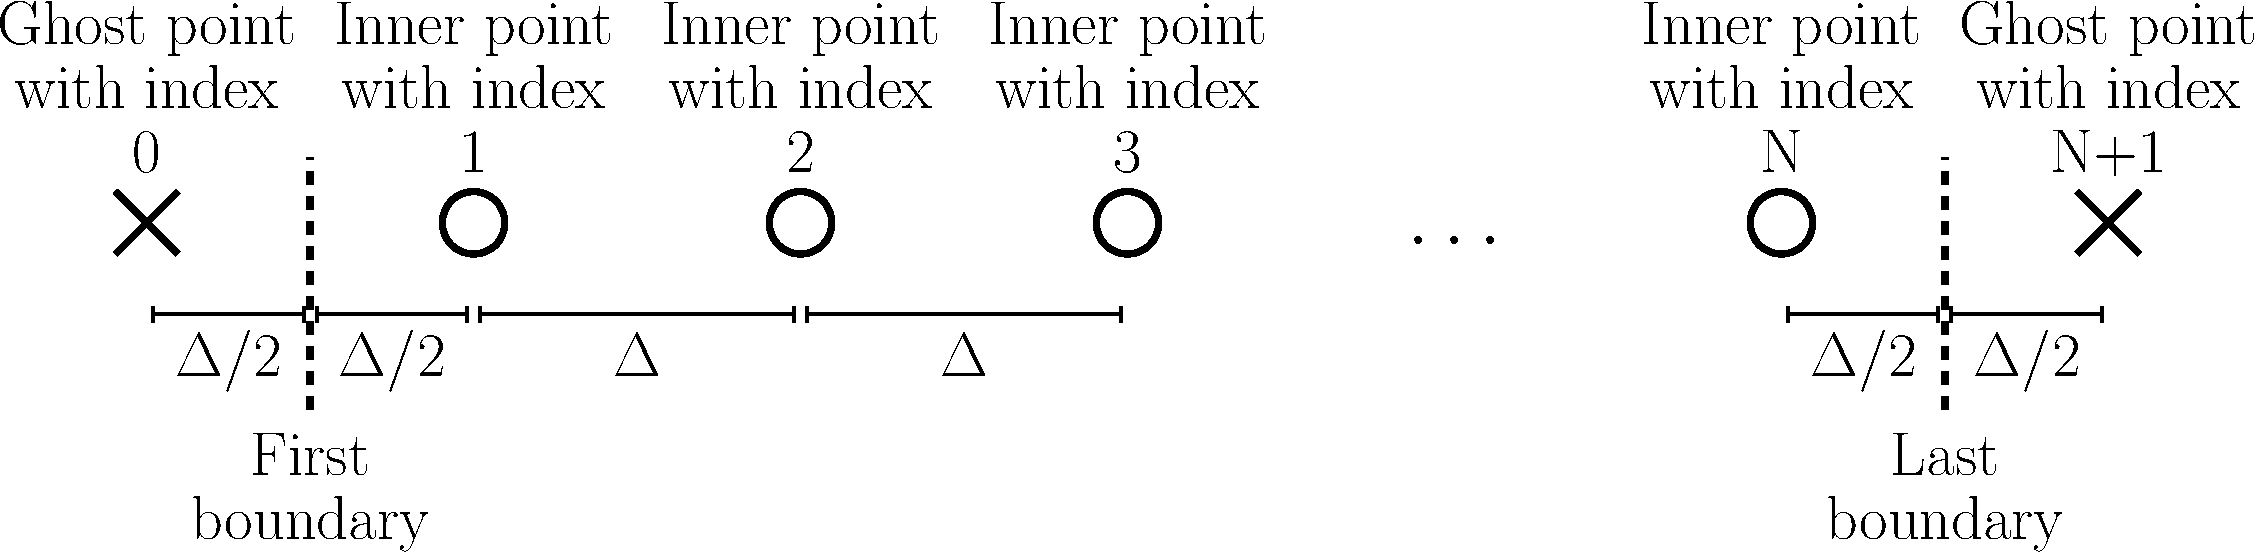
\includegraphics[width=1.0\textwidth]{fig/flatGrid}
    \caption{\textit{
            The boundaries ar positioned half between grid points.
            $\Delta$ denotes the grid spacing between two grid points.
        }}
    \label{fig:flatBC}
\end{figure}
%
The boundary condition given in \cref{fig:BCs} gives a value at the position of the boundary.
As there is no grid point at the boundary, the value is extrapolated to the ghost point $\frac{\Delta}{2}$.
For the Dirichlet boundary condition, the following $4$th order extrapolation %
%
\footnote{
Derived using a Newton polynomial (using the four points around the edge of the domain of \cref{fig:flatBC} (including the ghost point)), and evaluate it in the ghost point.
}%
is used
%
\begin{align*}
      f_{0} =& \frac{16}{5}f_{\text{First boundary}}
              - 3          f_1
              +            f_2
              - \frac{1}{5}f_3
    \\
      f_{N} =& \frac{16}{5}f_{\text{Last boundary}}
              - 3          f_{N}
              +            f_{N-1}
              - \frac{1}{5}f_{N-2}
\end{align*}
%
For the Neumann boundary condition a $4$th order extrapolation %
%
\footnote{
Derived using a one sided stencil (using the five points around the edge of the domain of \cref{fig:flatBC} (including the ghost point)) of the first derivate evaluated at the boundary, and solve for it for the ghost point.
% See D4DX4/BW2ndOrderNeumann4thOrder
}%
%
is used, reading
%
\begin{align*}
      f_0 =& \frac{12}{11}\Delta f_{\text{First boundary}}
                +
                \frac{
                  17f_1
                +  9f_2
                -  5f_3
                +   f_4
               }{22}
    \\
      f_{N+1} =& \frac{12}{11}\Delta f_{\text{Last boundary}}
                +
                \frac{
                  17f_{N}
                +  9f_{N-1}
                -  5f_{N-2}
                +   f_{N-3}
               }{22}
\end{align*}
%
In the cases where no boundary is imposed (for the parallel derivative of $\phi$ mentioned in \cref{sec:BCs} and in the composite derivatives mentioned in \cref{sec:compDeriv}), the following extrapolation %
%
\footnote{
Derived using a Newton polynomial (using the five points around the edge of the domain of \cref{fig:flatBC} (excluding the ghost point)), and evaluate it in the ghost point.
}%
is used for the ghost points
%
\begin{align}
    f_{N+1} =& 4f_{N} - 6f_{N-1} + 4f_{N-2} - f_{N-3},
    \label{eq:extraPolUp}
    \\
    f_{0} =& 4f_{1} - 6f_{2} + 4f_{3} - f_{4}
    \label{eq:extraPolDown}
\end{align}
%
Finally, as the $\theta$ direction is periodical, the ghost points are simply
%
\begin{align*}
    f_{N+1} =& f_{1}
    \\
    f_{0} =& f_{N}
\end{align*}

\section{Artificial viscosity}
\label{sec:art_visc}
%
As mentioned in \cref{sec:SOE}, we have neglected the viscosities (as we assume that these are small).
Instead, we add some artificial viscosities, which is needed for numerical stability (in addition to those added through the upwinding schemes).
If there are no viscosities in the system, there is no mechanism (other than diffusion) which can remove the small scales (structures with a short gradient scale length) from the system.
Scales which are smaller than what can be resolved by the grid will lead to problems like aliasing.
These small scales can then build up and make the simulation crash%
\footnote{
    We will here use the word "crash" meaning that the simulation stops because of bad behavior the numerics.
    The simulation stops if a field reaches $\pm$\texttt{inf} or \texttt{nan} values (this can cause division by zero problems) or if the solver takes too small time steps over a range of time because it cannot resolve unphysically large gradients.
}%
%
.

For this reason, we add viscosities on the form
%
\begin{align*}
    D_{f, \|, \text{art}} \nabla_{\|}^2 f
    + D_{f, \perp, \text{art}} \grad_\perp^2 f
    &=
    D_{f, \|, \text{art}} \div \L(\ve{b}\ve{b}\cdot\grad\R) f
    + D_{f, \perp, \text{art}} \grad_\perp^2 f
    \note{$\partial_i \ve{b} = 0$}
    \\
    %
    &=
    D_{f, \|, \text{art}} \ve{b}\cdot\grad \L(\ve{b}\cdot\grad\R) f
    + D_{f, \perp, \text{art}} \grad_\perp^2 f
    \\
    %
    &=
    D_{f, \|, \text{art}} \partial_\|^2 f
    + D_{f, \perp, \text{art}} \grad_\perp^2 f,
    \numberthis
    \label{eq:art_vort}
\end{align*}
%
to all the evolved fields $f$.

In addition, a hyper-viscous term is added in the azimuthal direction for the $\Om^D$ and $\Om$ equations.
This term is on the form
%
\begin{align*}
    - D_{f, \theta, \text{art}}^H \partial_{\theta}^4 f.
\end{align*}
%
The reason for this is that small scales grow up in the vorticity equations despite the filtering mentioned in \cref{sec:filt}.
To see that this term actually dampens higher modes, consider the example
%
\begin{align*}
    \partial_t f = (-1)^{m+1}D \partial_x^{2m} f \qquad m\in\mathbb{N},
\end{align*}
%
which we for simplicity assumes is periodical in $x$.
For a certain wave number $k$, we now have (see \cref{app:deriv_of_FT} for details)
%
\begin{align*}
    \partial_t f_k = (-1)^{m+1} (ik)^{2m} D f_k,
\end{align*}
%
where the $(-1)^{m+1}$ factor ensures that the time evolution of wave number $k$ is decreasing for every choice of $m$.
The artificial viscosity coefficients used in this thesis are given in \cref{tb:artVisc}.
%
\begin{table}[h!]
{\footnotesize \centerline{
\colorme
\begin{tabular}{c|ccc}
\hline\hline
%
Variable & $\qquad D_\|\qquad$ & $\qquad D_\perp\qquad$ & $\qquad D^{\text{Hyper}}_\theta\qquad$ \\
%
\hline
%
$\ln(n)$    & $ 40$ & $3.0\cdot10^{-3}$ & $0$\\
$nu_{i,\|}$ & $ 40$ & $3.0\cdot10^{-3}$ & $0$\\
$j_\|$      & $ 40$ & $3.0\cdot10^{-3}$ & $0$\\
$\Om^D$     & $0.1$ & $2.4\cdot10^{-4}$ & $5.81\cdot10^{-6}$\\
$\Om$       & $0.1$ & $2.4\cdot10^{-4}$ & $5.81\cdot10^{-6}$\\
%
\hline\hline
\end{tabular}
}}
\caption{
        Artificial viscosities used in the CELMA code.
        Artificial viscosities to $\Om^D$ is only added for the case where the Boussinesq approximation is \textbf{NOT} used.
        Artificial viscosities to $\Om$ is only added for the case where the Boussinesq approximation is used.
    }
    \label{tb:artVisc}
\end{table}
%

Higher coefficients are used in the parallel direction as the background gradients in this direction are much more gradual than the background gradients in the perpendicular gradients.
In the end, both $D_{f, \|, \text{art}} \partial_\|^2 f$ and $D_{f, \perp, \text{art}} \grad_\perp^2 f$ are small compared to the other terms.
% FIXME: Would be nice to showing a plot showing that the artificial terms are small
Notice that the artificial viscosities in $\Om^D$ and $\Om$ are smaller compared with the other fields.
This is because the vorticity is usually quite filamented, and large artificial viscosities will not only remove the small scales, but also alter the physical behavior of the system.

\section{Time solver}
This chapter will briefly discuss the time solver used in this thesis.
At the time of writing the following time solvers are available in the BOUT++ framework
% FIXME: Mention time solvers, and add references.

The \texttt{cvode}\cite{Hindmarsh2012book} has been found to be a robust and fast time solver for solving \cref{eq:celma_dens,eq:celma_mom_dens,eq:celma_j_par,eq:celma_vortD_evolution} in time.

As \cref{eq:celma_dens,eq:celma_mom_dens,eq:celma_j_par,eq:celma_vortD_evolution} contains no mixed temporal and spatial derivatives in the equations, the PDEs can first be discretized in the spatial dimension while keeping the time derivatives continuous.
The set of PDEs is thereby rewritten to a set of ODEs (one for each of the discretized point in space) which needs to be solved simultaneously.
This method is known as the "Method of Lines" (MOL) \cite{Leveque2007book}, and is widely used when solving a set of non-linear PDEs.

The problem can now be stated in the following way:
Let $\ve{f} = \{\ln(n), nu_{i,\|}, j_\|, \Om^D\}$, for $\ln(n)$, $nu_{i,\|}$, $j_\|$ and $\Om^D$ discretized in space.
That is, $\ve{f}$ is the tuple of the time dependent variables, and contains $\ln(n)_{0,0,0}$, $\ln(n)_{0,0,1}$ \ldots $\ln(n)_{n_\rho,n_z,n_\theta}$, \ldots $nu_{{i,\|}_{0,0,0}}$, \ldots $\Om^D_{n_\rho,n_z,n_\theta}$ where the subscripts denotes the grid index.
Hence, we would like to solve
%
\begin{align}
    \parti{\ve{f}(t)}{t} = F(\ve{f}),
    \label{eq:MOL}
\end{align}
%
for $\ve{f}$, where $F(\cdot)$ denotes the nonlinear operator which contains discretized differential operators in the spatial dimension.

\Cref{eq:MOL} can be stepped forward in time by using an appropriate time solver, like Runge-Kutta or a Linear Multistep Method (LMM).
Due to its good stability properties \cite{Leveque2007book} an implicit LMM has been chosen%
\footnote{
    Unless other is explicitly stated, \texttt{cvode}'s variable step size Backward Differentiation Formula (BDF) of variable order (1-5) has been chosen.
    This includes the STAbility Limit Detection (STALD) algorithm, which detect linear stability regions, and chooses the step-size thereby.
}
%
.

By using a generic LMM to \cref{eq:MOL}, we get
%
\begin{align*}
    \sum_{j=0}^{r}\a_j\ve{f}(t_{n+j}) =& k\sum_{j=0}^{r}\b_jF(\ve{f}(t_{n+j}), t_{n+j})\\
    %
    \a_r\ve{f}(t_{n+r}) + \sum_{j=0}^{r-1}\a_j\ve{f}(t_{n+j}) =&
    \b_rF(\ve{f}(t_{n+r}), t_{n+r}) +
    k\sum_{j=0}^{r-1}\b_jF(\ve{f}(t_{n+j}), t_{n+j})\\
    %
    \ve{f}(t_{n+r})
    -
    \frac{\b_r}{\a_r}F(\ve{f}(t_{n+r}), t_{n+r})
    =&
    \frac{k}{\a_r}\sum_{j=0}^{r-1}\b_jF(\ve{f}(t_{n+j}), t_{n+j})
    - \frac{1}{\a_r}\sum_{j=0}^{r-1}\a_j\ve{f}(t_{n+j}).
    \numberthis
    \label{eq:LMM}
\end{align*}
%
The method is implicit if $\b_r\neq0$.
That is, the solution for the next time step depends on the next time step itself.
In other words \cref{eq:LMM} can be stated as an optimization problem.
By defining $\frac{\b_r}{\a_r}\defined\gamma$, we have
%
\begin{align*}
    \ve{f}(t_{n+r})
    - \gamma F(\ve{f}(t_{n+r}), t_{n+r})
    - \frac{k}{\a_r}\sum_{j=0}^{r-1}\b_jF(\ve{f}(t_{n+j}), t_{n+j})
    + \frac{1}{\a_r}\sum_{j=0}^{r-1}\a_j\ve{f}(t_{n+j})
    =
    G(\ve{f}(t_{n+r}))
    =&
    0.
\end{align*}
%
Which we would like to solve for $\ve{f}(t_{n+r})$.
This can be done by using Newton Raphson's method.
I.e. we do a multivariate Taylor expansion of $G(\ve{f}(t_{n+r}))$ around an approximate point $\ve{f}_l(t_{n+r})$, and retain only the linear terms
%
\begin{align*}
    G(\ve{f}(t_{n+r})) \simeq
    G(\ve{f}_{l}(t_{n+r})) + \L(\parti{ G(\ve{f}_{l}(t_{n+r})) }{\ve{f}_{l}(t_{n+r})}\R)
    \L(\ve{f}(t_{n+r}) - \ve{f}_{l}(t_{n+r})\R),
\end{align*}
%
as $ G(\ve{f}(t_{n+r})) = 0$, we get
%
\begin{align*}
    0 \simeq
    G(\ve{f}_{l}(t_{n+r})) + \L(\parti{ G(\ve{f}_{l}(t_{n+r})) }{\ve{f}_{l}(t_{n+r})}\R)
    \L(\ve{f}(t_{n+r}) - \ve{f}_{l}(t_{n+r})\R).
\end{align*}
%
The solution $\ve{f}(t_{n+r})$ to this problem can then serve as the next iteration, so that
%
\begin{align*}
    \ve{f}_0(t_{n+r}) =& \ve{f}(t_{n+r-1})\\
    \ve{f}_{l+1}(t_{n+r}) =& \ve{f}_l(t_{n+r})-
    \L(\parti{ G(\ve{f}_{l}(t_{n+r})) }{\ve{f}_{l}(t_{n+r})}\R)^{-1}
    G(\ve{f}_{l}(t_{n+r})),
\end{align*}
%
where $l$ denote the $l^{\text{th}}$ Newton iteration.
The iterations can be rewritten to
%
\begin{align}
    \parti{ G(\ve{f}_{l}(t_{n+r})) }{\ve{f}_{l}(t_{n+r})}
    \L( \ve{f}_{l+1}(t_{n+r}) - \ve{f}_l(t_{n+r}) \R)
    =&
    -G(\ve{f}_{l}(t_{n+r})),
    \label{eq:newtonIt}
\end{align}
%
where
%
\begin{align*}
    \parti{ G(\ve{f}(t_{n+r})) }{\ve{f}(t_{n+r})}
    =&
    \parti{ }{\ve{f}(t_{n+r})}
    \L(
    \ve{f}(t_{n+r})
    - \gamma F(\ve{f}(t_{n+r}), t_{n+r})
    - \frac{k}{\a_r}\sum_{j=0}^{r-1}\b_jF(\ve{f}(t_{n+j}), t_{n+j})
    + \frac{1}{\a_r}\sum_{j=0}^{r-1}\a_j\ve{f}(t_{n+j})
    \R)
    \\
    =&
    \mathbb{I}
    - \gamma\parti{F(\ve{f}(t_{n+r}), t_{n+r})}{\ve{f}(t_{n+r})}
    \\
    =&
    \mathbb{I} - \gamma\mathbb{J}.
    \numberthis
    \label{eq:AInNewton}
\end{align*}
%
By inserting \cref{eq:AInNewton} in \cref{eq:newtonIt}, we get
%
\begin{align*}
    \L( \mathbb{I} - \gamma\mathbb{J}\R)
    \L( \ve{f}_{l+1}(t_{n+r}) - \ve{f}_l(t_{n+r}) \R)
    =&
    -G(\ve{f}_{l}(t_{n+r})).
\end{align*}
%
which can be recast to
%
\begin{align}
    A \ve{x} =& \ve{b}.
    \label{eq:newtonInverse}
\end{align}
%
In other words, we need to invert $A$ (that is $\L( \mathbb{I} - \gamma\mathbb{J}\R)$) for each Newton iteration.
As the system of equations in \cref{eq:newtonInverse} is rather large (and also generally non-symmetric), a robust an fast method is sought to solve for $\ve{x}$.
This can be done by using the \textbf{G}eneralized \textbf{M}inimal \textbf{RES}idual method (GMRES).

% NOTE: Finding the Krylov subspace is almost like using the von Mises (power iteration method) of finding the eigenvector with the highest eigenmode
This method approximates the exact solution of \cref{eq:newtonInverse} by a vector in the Krylov subspace (spanned by vectors obtained through the Arnoldi process), which minimizes the residual $\ve{r}_n = A \ve{x}_n - \ve{b}$. See \cite{Saad2003book} for details.

One of the advantages is that the Jacobian for the GMRES needs not to be expanded in memory as the Arnoldi process only needs to evaluate a Jacobian vector product \cite{Knoll2004}.

The method is also easily preconditioned%
\footnote{
    To precondition means to find a $P_L$ and/or $P_R$, which is easy to invert, and makes either $(P_L^{-1}A) \ve{x} = P_L^{-1}\ve{b}$, $(A P_R^{-1})P_R\ve{x} = \ve{b}$ or $(P_L^{-1}AP_R^{-1}) \ve{x} = P_L^{-1}\ve{b}$ numerically easier to solve than \cref{eq:newtonInverse}, as the matrices in parentheses is used in finding vectors spanning the Krylov subspace rather than $A$ itself.
}
%
, as shown in \cite{Dudson2012}.
Although preconditioning is expected to give substantial speed-ups \cite{Hindmarsh2012book}, it is outside the scope of this thesis.

In this thesis, the options for the time solver is given in \cref{tb:timeSolve}.
%
\begin{table}[h!]
{\footnotesize \centerline{
\colorme
\begin{tabular}{c|l}
\hline\hline
%
Variable & Value\\
%
\hline
%
Absolute tolerance              & $1.0\cdot10^{-10}$\\
Relative tolerance              & $1.0\cdot10^{-5} $\\
Max allowed iterations per step & $1.0\cdot10^{8}  $\\
%
\hline\hline
\end{tabular}
}}
\caption{Time solver options used in the CELMA code.}
\label{tb:timeSolve}
\end{table}
%
% FIXME: Mention that IMEX has been tried out, but has not worked

\chapter{Additional implementations}
\label{chap:additionalImplementation}
We will in this chapter describe additional implementations to the CELMA code, which (at the time of writing) is not included in the BOUT++ framework.

\section{Composite derivatives}
%
In \cref{eq:celma_dens,eq:celma_mom_dens,eq:celma_j_par,eq:celma_vortD_evolution} and \cref{eq:celma_vort_boussinesq} there are some terms which are written as a combination of two or more FDs.
These are
%
\begin{align*}
    &\{\phi,\cdot\},&
    &\{\ve{u}_E^2,n\},&
    &\partial_\|\div \L( u_{i,\|}n \frac{\grad_\perp \phi}{B}\R)&
    &\text{and}&
    &\div \L( S_n \L[ \frac{ \grad_\perp \phi }{ B } \R] \R)&
\end{align*}
%
These can either be calculated by applying two (or more) different FDs consecutively to a field $f$, or by making a new FD stencil specifically for the operator under consideration.

Special care must be taken at the ghost points if one choose to apply two (or more) different FDs consecutively.
To see this, we can call $g$ the result of calculating the FD of a field $f$.
As we are using centred stencils (as described in
% FIXME: Add reference to the FD stencils used
), then the ghost points of $g$ is not calculated by the FD%
%
\footnote{There is by definition no way to apply a centred stencil to the last grid point.}%
%
\footnote{One could in principle use a one-sided stencil on the ghost points $f$ when calculating the FD of $f$, so that the ghost point of $g$ would be known.
This is however not done here.}
%
.

\subsection{Arakawa's stencil}
%
As already noted in \cref{sec:vecAdvTerm}, we can write $\ve{E}\times\ve{B}$-advective terms (that is the $\{\phi,\cdot\}$ terms) as Poisson brackets.
The proof is found in \cref{app:poisson}.
The benefits of writing terms on Poisson brackets are presented in Arakawa's paper from 1966 \cite{Arakwa1966}.
In short, the paper shows that a na\"ive FD discretization of the Poisson bracket does not conserve energy and enstrophy.
At the same time it gives an alternative way of discretize in orthogonal curvilinear coordinates in order to keep these quantities conserved.
If the energy and enstrophy is not conserved, fake generation of these quantities occur, which eventually will lead to a blow up of the simulation (in a way described by Phillips in \cite{Phillips1959}).

\subsection{Advection by \texorpdfstring{$\ve{u}_E^2$}{the squared E cross B drift}}
\label{sec:ExBadv}
%
It is also possible to discretize the term $\{\ve{u}_E^2, n\}$ using Arakawa's method.
We observe that in cylindrical coordinates, we have
%
\begin{align*}
    \{\ve{u}_E^2, n\} &= \L\{\L(\frac{\grad_\perp \phi}{B}\R)^2, n\R\}
    \note{Constant $B$}
    \\
    %
    &= \L(\frac{1}{B}\R)^2
    \L\{\L(\L[\ve{e}^{\rho}\partial_{\rho} + \ve{e}^{\theta}\partial_{\theta}\R] \phi\R)
        \cdot
        \L(\L[\ve{e}^{\rho}\partial_{\rho} + \ve{e}^{\theta}\partial_{\theta}\R] \phi\R)
        , n\R\}
    \note{Orthogonality}
    \\
    %
    &= \L(\frac{1}{B}\R)^2
    \L\{g^{\rho\rho}\L(\partial_{\rho} \phi\R)^2+
        g^{\theta\theta}\L(\partial_{\theta} \phi\R)^2
        , n\R\}
    \\
    %
    &= \L(\frac{1}{B}\R)^2
    \L\{\L(\partial_{\rho} \phi\R)^2+ \frac{1}{\rho^2}\L(\partial_{\theta} \phi\R)^2
        , n\R\}
\end{align*}
%
Here, we must take care when we treat the ghost points.
No ghost points is needed in the $\theta$ direction, as this direction is periodic.
Thus, for $\partial_{\theta} \phi$, we only need to make sure that we take the $\theta$ derivatives at the ghost points in $\rho$.

For $\partial_{\rho} \phi$, we must re-apply the values in the $\rho$ ghost points as the derivative is not calculated there.
For the inner ghost point, the same procedure as used in \cref{sec:ghostRhoDeriv} can be used.
For the outer ghost point, we can use \cref{eq:extraPolUp} for extrapolation to the ghost point.

This way of discretizing is second order accurate, as indicated in MES
%FIXME: Refer to table or so in MES


\subsection{\texorpdfstring{$\div(g\grad_\perp f)$}{Divergence of g times the perpendicular gradient of f} terms}
%
We have that
%
\begin{align*}
    \div(f\nabla_\perp g)
    =& f\grad_\perp^2g + \grad f\cdot       \grad_\perp g
    \\
    =& f\grad_\perp^2g + \grad_\perp f\cdot \grad_\perp g
    \note{See \cref{sec:perpLapl}}
    \\
    =&
    f\L(g^{ij} \partial_i \partial_j + G^j \partial_j -\frac{1}{J} \partial_z \L(\frac{J}{g_{zz}} \partial_2\R)\R)g
    +
    \L(e^\rho \partial_\rho  + e^\theta \partial_\theta \R)f\cdot \L(e^\rho \partial_\rho  + e^\theta \partial_\theta \R)g
    \\
    =&
    f\L(g^{ij} \partial_i \partial_j + G^j \partial_j -\frac{1}{J} \partial_z \L(\frac{J}{g_{zz}} \partial_2\R)\R)g
    +
    g^{\rho\rho} \partial_\rho f \partial_\rho g
    +
    g^{\rho\theta} \partial_\rho f  \partial_\theta g
    +
    g^{\theta\rho} \partial_\theta f  \partial_\rho g
    +
    g^{\theta\theta} \partial_\theta f \partial_\theta g
    \numberthis
    \label{eq:perpPerpDeriv}
\end{align*}
%
As BOUT++ includes a numerical opertor for $\grad_\perp^2g$ (as mentioned in \cref{sec:perpLapl}), we could have used this operator for calculating $f\grad_\perp^2g$.
However, from \cref{app:coord}, we that
%
\begin{align*}
  G^\rho =& \frac{1}{J}\\
  G^z =& 0\\
  G^\theta =& 0\\
  g^{ij} =& 0 \qquad i\neq j\\
  g^{\rho\rho} =& 1\\
  g^{\theta\theta} =& \frac{1}{\rho^2}\\
  g^{zz}\partial_z^2 - \frac{1}{J}\partial_z\left(\frac{J}{g^{zz}}\partial_z\right) =& 0,
\end{align*}
%
in cylindrical coordinates.
Thus \cref{eq:perpPerpDeriv} can be rewritten to
%
\begin{align*}
    &f\L(g^{\rho\rho} \partial_\rho \partial_\rho + g^{\theta\theta} \partial_\theta \partial_\theta + G^\rho \partial_\rho \R)g
    + g^{\rho\rho} \partial_\rho f \partial_\rho g
    + g^{\theta\theta} \partial_\theta f \partial_\theta g
    \\
    =&
    f \partial^2_\rho g
    + f \frac{1}{\rho^2}\partial^2_\theta g
    + f\frac{1}{\rho}\partial_\rho g
    +  \partial_\rho f \partial_\rho g
    +  \frac{1}{\rho^2} \partial_\theta f \partial_\theta g
\end{align*}
%
%FIXME: Has this been MESed?
%
which is what is implemented for this operator in the CELMA code.

\subsection{Parallel derivative of the divergence of the cross term}
%
As $\partial_\|\div \L( u_{i,\|}n \frac{\grad_\perp \phi}{B}\R)$ can be rewritten to $\partial_\|\div(g\grad_\perp f)$, we just have to take care of the parallel ghost points of $\div \L( u_{i,\|}n \frac{\grad_\perp \phi}{B}\R)$ before taking the parallel derivate.
We can use \cref{eq:extraPolUp} for calculation of the upper ghost point, and \cref{eq:extraPolDown}  for calculation of the lower ghost point.


%FIXME: Add these polynomials in additional implementations
Along a grid, index of the last ghost point along the grid given as $N+1$, counting from $0$ where $-1$ is the index of first ghost point.
See figure
-1           1         2     N   N+1
o |          x         x ... x | o
    |------|  |------|
 BC delta/2     delta          BC

\begin{align}
    f_{N+1} = 4f_{N} - 6f_{N-1} + 4f_{N-2} - f_{N-3}
    \label{eq:extraPolUp}
\end{align}
%
lol
%
\begin{align}
    f_{-1} = 4f_{0} - 6f_{1} + 4f_{2} - f_{3}
    \label{eq:extraPolDown}
\end{align}

\section{Extrapolation to the ghost point}
\label{sec:extrapolGhost}
%
In the cases where no boundary is imposed (for the parallel derivative of $\phi$ mentioned in \cref{sec:BCs} and in the composite derivatives mentioned in \cref{sec:compDeriv}), the following extrapolation %
%
\footnote{
Derived using a Newton polynomial (using the five points around the edge of the domain of \cref{fig:flatBC} (excluding the ghost point)), and evaluate it in the ghost point.
}%
is used for the ghost points
%
\begin{align}
    f_{N+1} =& 4f_{N} - 6f_{N-1} + 4f_{N-2} - f_{N-3}
    \label{eq:extraPolUp}
    \\
    f_{0} =& 4f_{1} - 6f_{2} + 4f_{3} - f_{4},
    \label{eq:extraPolDown}
\end{align}
%
where the indices the ones indicated at \cref{fig:flatBC}.

\section{Obtaining \texorpdfstring{$\phi$}{the potential}}
%
We observe the dependency of $\phi$ in \cref{eq:celma_dens,eq:celma_mom_dens,eq:celma_j_par,eq:celma_vortD_evolution}, but that $\phi$ is not described by a initial boundary value problem equation.
Instead, we must find alternative ways of extracting $\phi$.
We will in the following discuss two ways of doing so.
% TODO: Delete me if not in thesis
%       extra/constraint can be inserted here

\subsection{As a matrix inversion problem}
%
The problem of obtaining $\phi$ can be posed as a matrix problem $A\ve{x}=\ve{b}$, where $\ve{x}$ is an array of all the spatial values of $\phi$ ordered in some way, and $\ve{b}$ is an array of all the spatial values of $\Omega^D$ ordered in the same way.
Since we are working in an orthogonal coordinate system, we have that $\Om^D = \div\L(n\frac{\grad_\perp\phi}{B}\R) = \grad_\perp\cdot\L(n\frac{\grad_\perp\phi}{B}\R)$, as no basis vector parallel to the magnetic field can be obtained from taking the derivative of the vector $n\frac{\grad_\perp\phi}{B}$, which has only perpendicular components.
Thus, in our case, we can solve the $A\ve{x}=\ve{b}$ system for each plane perpendicular to the magnetic field.
That is, our matrix $A$ would be a $n_x \times n_y$ matrix, where $n_x$ and $n_y$ is the number of points for the two perpendicular directions
%
\footnote{
Note that in the BOUT++ implementation, $y$ is chosen as the direction parallel to the magnetic field.
This is due to historical reasons.
$n_y$ would be named $n_z$ in BOUT++ convention.
In order not to confuse readers unfamiliar with BOUT++, $z$ is chosen as the coordinate along the magnetic field unless other is specified.
}%
%
.
We note that if $\div\L(n\frac{\grad_\perp\phi}{B}\R)$ were not purely perpendicular, we would have to solve $A\ve{x}=\ve{b}$ for the whole domain.
In other words, the size of matrix $A$ would be $n_x \times n_y \times n_z$, and would be considerably harder to solve numerically.

As noted in \cite{Wiesenberger2014Phd} (in the case where $P=1$, that is, in the finite difference case), the discretization of the elliptic equation $\div\L(n\frac{\grad_\perp\phi}{B}\R)=\Om^D$ can be formulated in a symmetric manner, when special care is taken at the boundary.

Solving for the ghost-point, meaning that the ghost-point would be one of the unknown in $A\ve{x}=\ve{b}$, would break the symmetry.
Instead, one must reformulate the boundary condition in a way such that it becomes an equation for the ghost point.
The equation of the ghost point can then be substituted into the equations for the first/last inner point (the point just before the boundary) and thus effectively eliminating the ghost point from the set of equations.

To exemplify, consider a second order Dirichlet boundary condition with the boundary half between grid points for the equation $\partial_x^2 f = b$, where $f_{-1}$ denotes the value at the ghost point, $f_{\text{BC}}$ denotes the value at the boundary and $f_{1}$ denotes the value at the first inner ghost point.
The boundary condition can now be written $\frac{f_{-1}+f_{1}}{2}=f_{\text{BC}}$, and the equation for the first inner point could be written $\frac{f_{-1}+2f{1}+f_{2}}{(\Delta x)^2}=b_1$.
This would lead to the equation system
%
\begin{align*}
    A\cdot\ve{f}=&\ve{b}\\
    %
    \frac{1}{(\Delta x)^2}
    \begin{bmatrix}
        (\Delta x)^2\frac{1}{2} & (\Delta x)^2\frac{1}{2} & 0 & 0 & \ldots\\
        1                       & 2                       & 1 & 0 & \ldots\\
        0                       & 1                       & 2 & 1 & \ldots\\
        \vdots                  & \vdots              &\vdots&\vdots&\ddots\\
    \end{bmatrix}
    \cdot
    \begin{bmatrix}
        f_{-1}\\
        f_{1}\\
        f_{2}\\
        f_{3}\\
        \vdots
    \end{bmatrix}
    =&
    \begin{bmatrix}
        f_{\text{BC}}\\
        b_{1}\\
        b_{2}\\
        b_{3}\\
        \vdots
    \end{bmatrix}
\end{align*}
%
which is clearly non-symmetric.

The symmetric way to implement this would be to write $f_{-1}=2f_{\text{BC}}-f_{1}$ for the boundary condition, and substitute this into the 2nd order finite difference equation for the first inner ghost point.
This gives
%
\begin{align*}
    \frac{f_{-1}+2f{1}+f_{2}}{(\Delta x)^2}&=b_1\\
    \frac{2f_{\text{BC}}-f_{1}+2f{1}+f_{2}}{(\Delta x)^2}&=b_1\\
    \frac{f{1}+f_{2}}{(\Delta x)^2}&=b_1 - \frac{2f_{\text{BC}}}{(\Delta x)^2}
\end{align*}
%
This would give
%
\begin{align*}
    A\cdot\ve{f}=&\ve{b}\\
    %
    \frac{1}{(\Delta x)^2}
    \begin{bmatrix}
        1                       & 1                       & 0 & 0 & \ldots\\
        1                       & 2                       & 1 & 0 & \ldots\\
        0                       & 1                       & 2 & 1 & \ldots\\
        \vdots                  & \vdots              &\vdots&\vdots&\ddots\\
    \end{bmatrix}
    \cdot
    \begin{bmatrix}
        f_{1}\\
        f_{2}\\
        f_{3}\\
        \vdots
    \end{bmatrix}
    =&
    \begin{bmatrix}
        b_{1} - \frac{2f_{\text{BC}}}{(\Delta x)^2}\\
        b_{2}\\
        b_{3}\\
        \vdots
    \end{bmatrix}
\end{align*}
%
which is symmetric.
Although difficult, one can show that the non-linear elliptic equation in its symmetric form can be singular positive definite and thus be solved using the conjugate gradient method.
% FIXME: Add reference

\subsection{The Naulin solver}
%
The potential can also be found in an iterative way.
The method first used by Naulin in \cite{Naulin2008} will be presented here, and will be referred to as the Naulin solver.

The method can be used as long as
%
\begin{enumerate}[noitemsep,nolistsep]
    \item $\div\L(\frac{\grad_\perp\phi}{B}\R) = \frac{\grad_\perp^2\phi}{B}$
    \item $\grad f \cdot \grad_\perp g = \grad_\perp f \cdot \grad_\perp g$
\end{enumerate}
%
Point 1. is satisfied in our system as $B$ is constant, and because derivatives of the perpendicular basis vectors does not yield parallel components in our system.
Point 2. is satisfied as the dot product of the perpendicular basis vectors and the parallel basis vector is zero.
We then get that
%
\begin{align*}
    \Om^D =& \div\L(n\frac{\grad_\perp\phi}{B}\R)\\
    %
    =& n\div\L(\frac{\grad_\perp\phi}{B}\R) +
    \frac{\grad_\perp\phi}{B}\cdot\grad n
    \\
    %
    =& n\frac{\grad_\perp^2\phi}{B} +
    \grad n\cdot\frac{\grad_\perp\phi}{B}
    \\
    %
    =& n\frac{\grad_\perp^2\phi}{B} +
    \grad_\perp n\cdot\frac{\grad_\perp\phi}{B}
    \\
    %
    \Om^D =& n\frac{\grad_\perp^2\phi}{B} +
    \grad_\perp n\cdot\frac{\grad_\perp\phi}{B}
    \\
    %
    \frac{\Om^D}{n} =& \Om +
    \frac{1}{n}\grad_\perp n\cdot\frac{\grad_\perp\phi}{B}
    \\
    %
    \Om =& \frac{\Om^D}{n} -
    \grad_\perp \ln(n) \cdot\frac{\grad_\perp\phi}{B}
\end{align*}
%
Using square bracket superscript as iteration number, the algorithm can be stated in the following way:
%
\begin{algorithm}
\begin{enumerate}[noitemsep,nolistsep]
    \item Calculate
        $ \Om^{[i]} = \frac{\Om^D}{n} -
        \grad_\perp \ln(n) \cdot\frac{\grad_\perp\phi^{[i]}}{B}
        $
    \item Invert $\grad_\perp^2 \frac{\phi^{[i+1]}}{B} = \Om^{[i]}$ by the method
        described in \cref{app:lapInv}.
    \item Calculate
        $E_{\text{abs}, L_\infty} = \max \L|\phi^{[i]} - \phi^{[i+1]}\R|$
        and
        $E_{\text{rel}, L_\infty} = \max \L|\frac{\phi^{[i]} - \phi^{[i+1]}}{\phi^{[i]}}\R|$
    \item Check whether $E_{\text{abs}, L_\infty} > \text{Tolerance}_\text{abs}$
    \begin{itemize}[noitemsep,nolistsep]
        \item If yes: Check $E_{\text{abs}, L_\infty} > \text{Tolerance}_\text{rel}$
            \begin{itemize}[noitemsep,nolistsep]
                \item If yes: Assign $\phi^{[i+1]} \to \phi^{[i]}$, increase the
                    iteration number, throw an error if the iteration number is
                    above a predefined max iteration number, if not repeat from
                    step 1.
                \item Else, if no: Stop. Function returns
            \end{itemize}
        \item Else, if no: Stop. Function returns
    \end{itemize}
\end{enumerate}
\end{algorithm}
%
The inversion algorithm requires inner and outer boundary condition in the radial direction of $\phi$.
The outer boundary condition is described in \cref{sec:outerBC}, whereas the inner boundary condition is described in \cref{sec:innerPhiBC}.
\cref{tb:Naulin} states the options used in this thesis.
%
\begin{table}[h!]
{\footnotesize \centerline{
\begin{tabular}{c|l}
\hline\hline
%
Variable & Value\\
%
\hline
%
Absolute tolerance     & $1.0\cdot10^{-10}$\\
Relative tolerance     & $1.0\cdot10^{-5} $\\
Max allowed iterations & $1.0\cdot10^{6}  $\\
%
\hline\hline
\end{tabular}
}}
\caption[]{\textit{
        Naulin solver options used in the CELMA code.
    }}
\protect\label{tb:Naulin}
\end{table}

\section{Treatment of the singularity}
\label{sec:innerCenter}
The cylindrical coordinate system has a singularity at the axis (where $\rho=0$).
In other words, functions are not well defined in this point, and hence it is a bad idea to have a grid point there.
One way to avoid this problem is to put the grid points close to, but not at the very axis.
At the same time, as mentioned in \cref{sec:BCInnerRho}, there is a need of artificial boundary conditions as the domain covers $\rho \in \;]0, L_\rho[$.

\subsection{Ghost point for the radial derivative}
\label{sec:ghostRhoDeriv}
We immediatley observe that having a boundary condition at the singularity is a bad idea due to the singularity.
It is also a bad idea to use one sided FD schemes around this point, as this will prevent communication of information through the axis.

One way to circumvent the problem is to put the innermost point in rho $\Delta \rho$ appart from each other, where $\Delta \rho$ is the grid spacing.
I. e. the innermost points are both located $\frac{\Delta \rho}{2}$ from the axis, diametrically opposite of each other, as depicted on \cref{fig:innerRho}.
%
\begin{figure}[htb]
    \centering
    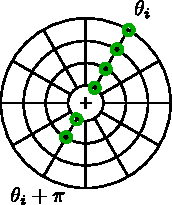
\includegraphics[width=0.5\textwidth]{fig/innerGhost}
    \caption{\textit{
The solid lines black lines represent the coordinate curves of a mesh with $4$ points in the $\rho$ direction (excluding the outermost ghost point depicted with a dashed black line), and $8$ points in the $\theta$-direction.
The green solid circles represents the inner grid points at $\theta=\theta_i$, with the corresponding ghost points at $\theta=\theta_i + \pi$ depicted in green dashed circles.
    }}
    \label{fig:innerRho}
\end{figure}
%
In this solution, the ghost points for the innermost grid points in $\rho$ (those closest to the singularity) will be set to the value of the innermost grid point which lies $\theta + \pi$ away.
The next ghost point will be set to the value of the second innermost internal point which lies $\theta + \pi$ away, and so on.
In this thesis, only one ghost point is used.
With this method the second order FD stencil for the radial derivative becomes
%
\begin{align*}
    \L.\parti{f}{\rho}\R|_{\rho=\frac{\Delta \rho}{2}} \simeq
    \frac{-f\L(-\frac{\Delta \rho}{2}, \theta\R) + f\L(\frac{3\Delta \rho}{2}, \theta\R)}{2\Delta \rho}
    =
    \frac{-f\L(\frac{\Delta \rho}{2}, \theta+\pi\R) + f\L(\frac{3\Delta \rho}{2}, \theta\R)}{2\Delta \rho}
\end{align*}
%
for the innermost point.
This method was used in \cite{Naulin2008}, and is second order convergent for a second order stencil as shown in \cref{sec:MES}.

\subsection{The inner boundary condition for \texorpdfstring{$\phi$}{the potential}}
\label{sec:innerPhiBC}
%
We also need an artificial ghost point for the innermost point in $\rho$ for inversion method described in \cref{app:lapInv}.
As the inversion in the $\rho$ direction will be done for each mode, the method described in \cref{sec:ghostRhoDeriv} is not directly applicable.

A method to do this, is to set the inner ghost point depending on the evenness of the mode.

If the mode is even, the mode under consideration would have the same value diametrically opposite of the innermost point.
Notice that this is true for every point sitting on the same radius.
Hence, the ghost point for the inner $\rho$ value is set to the same as the value at the innermost $\rho$.

If the mode is odd, the mode under consideration would have value of the point diametrically opposite of the innermost point, but with a changed sign.
Thus, the ghost point for the inner $\rho$ value is set to the negative of the value at the innermost $\rho$.
This is depicted in \cref{fig:BCLaplace}, and was first used in
%
\begin{figure}[h!]
    \centering
    \begin{subfigure}[t]{0.5\textwidth}
        \centering
        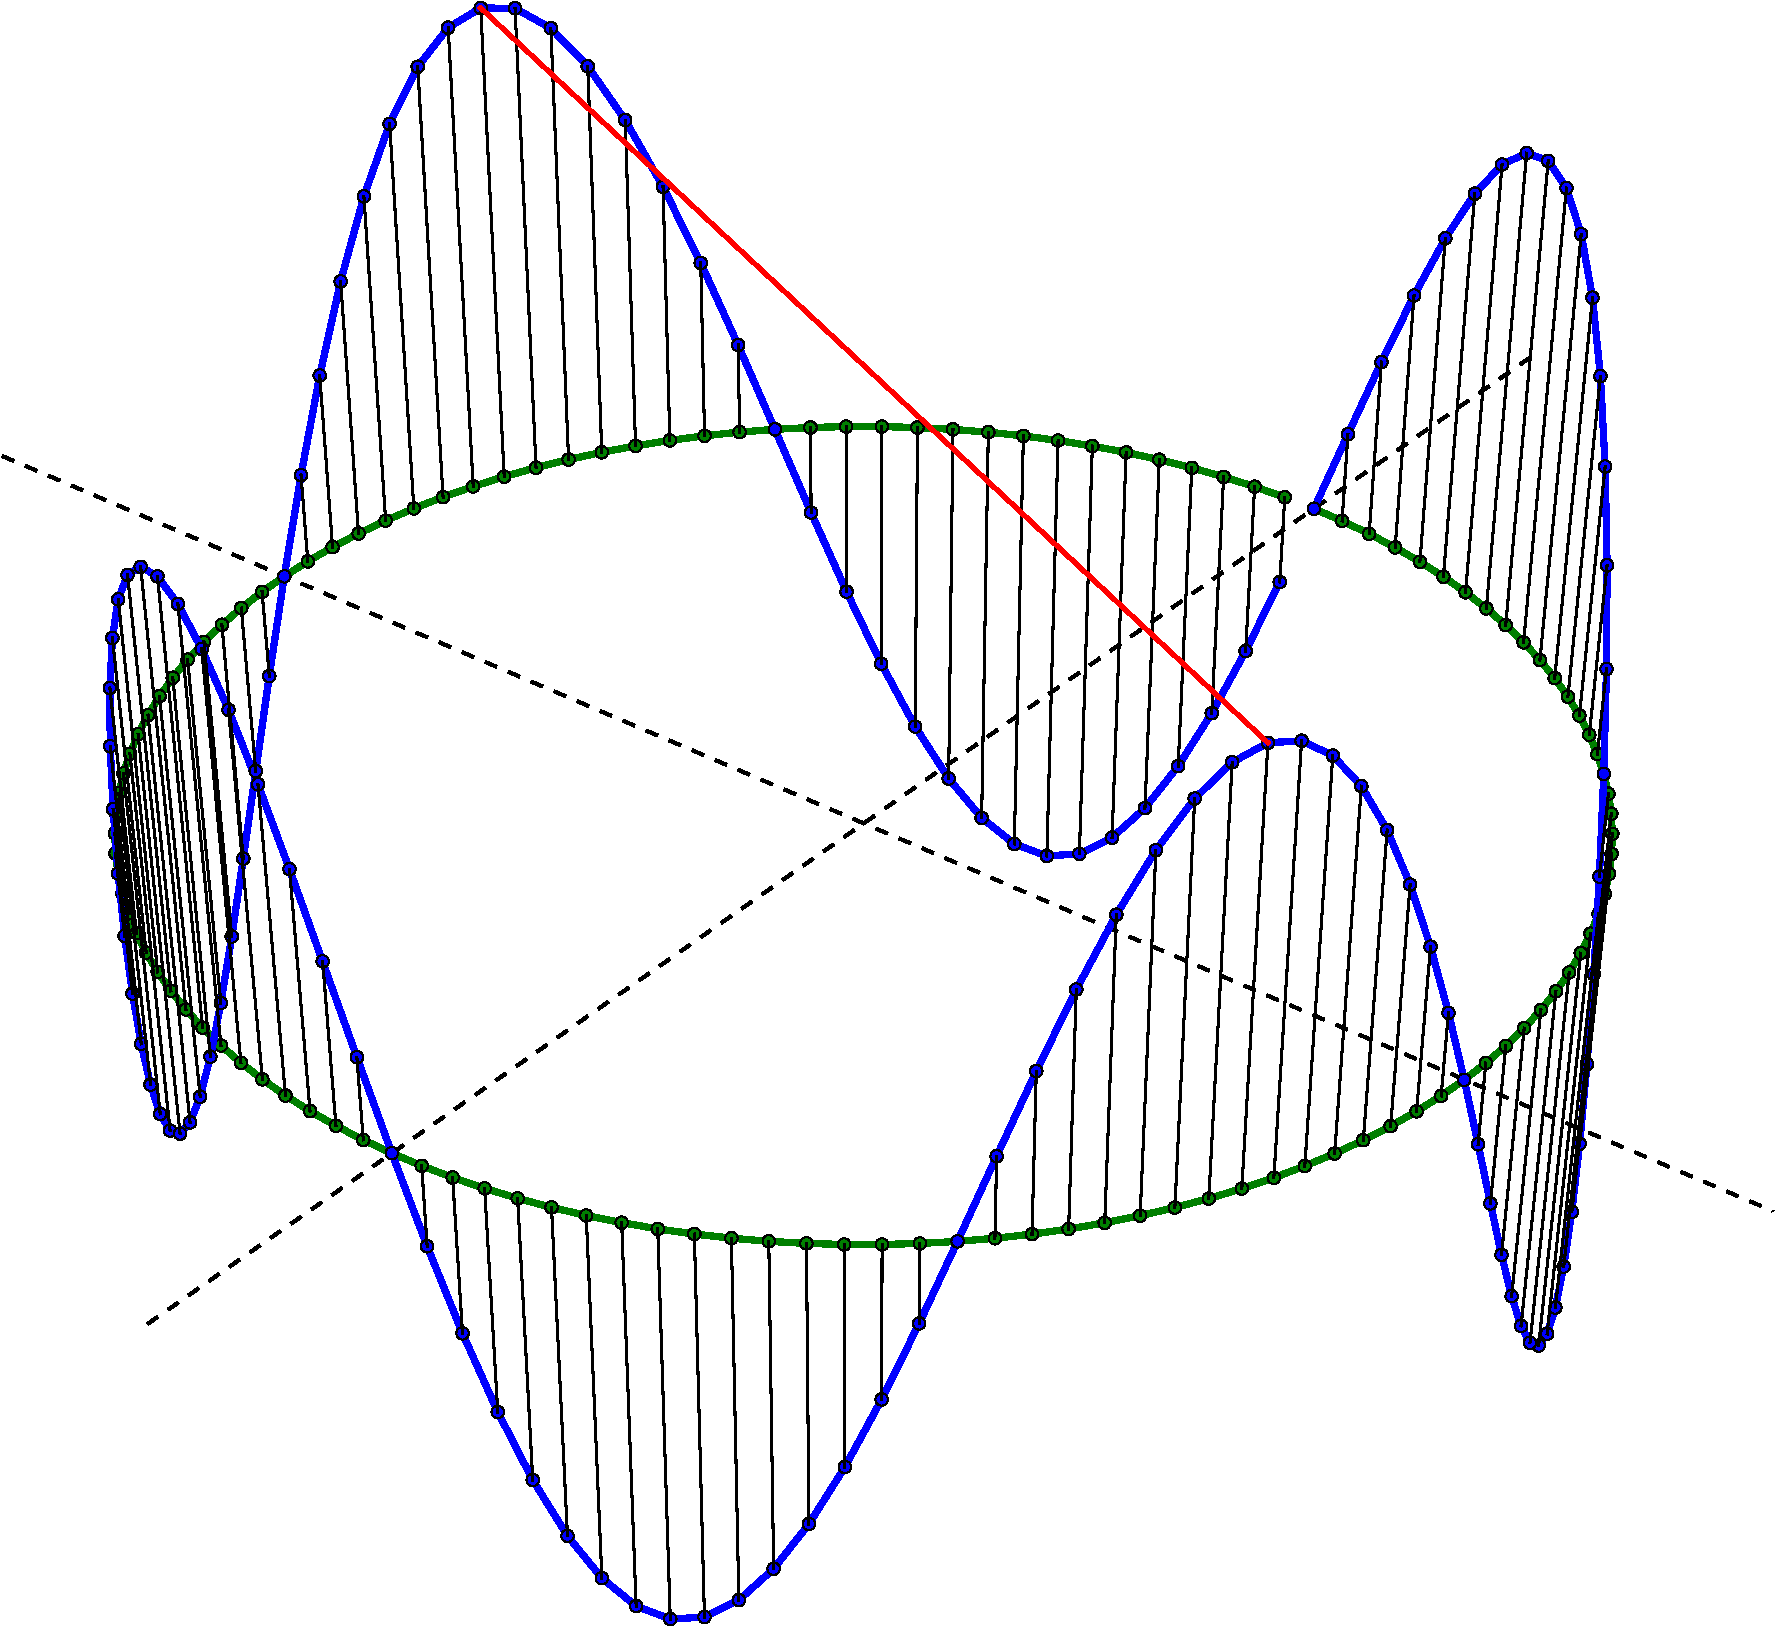
\includegraphics[width=0.8\textwidth]{fig/mode_4}
        \caption{An even mode.}
    \end{subfigure}%
    \hfill
    \begin{subfigure}[t]{0.5\textwidth}
        \centering
        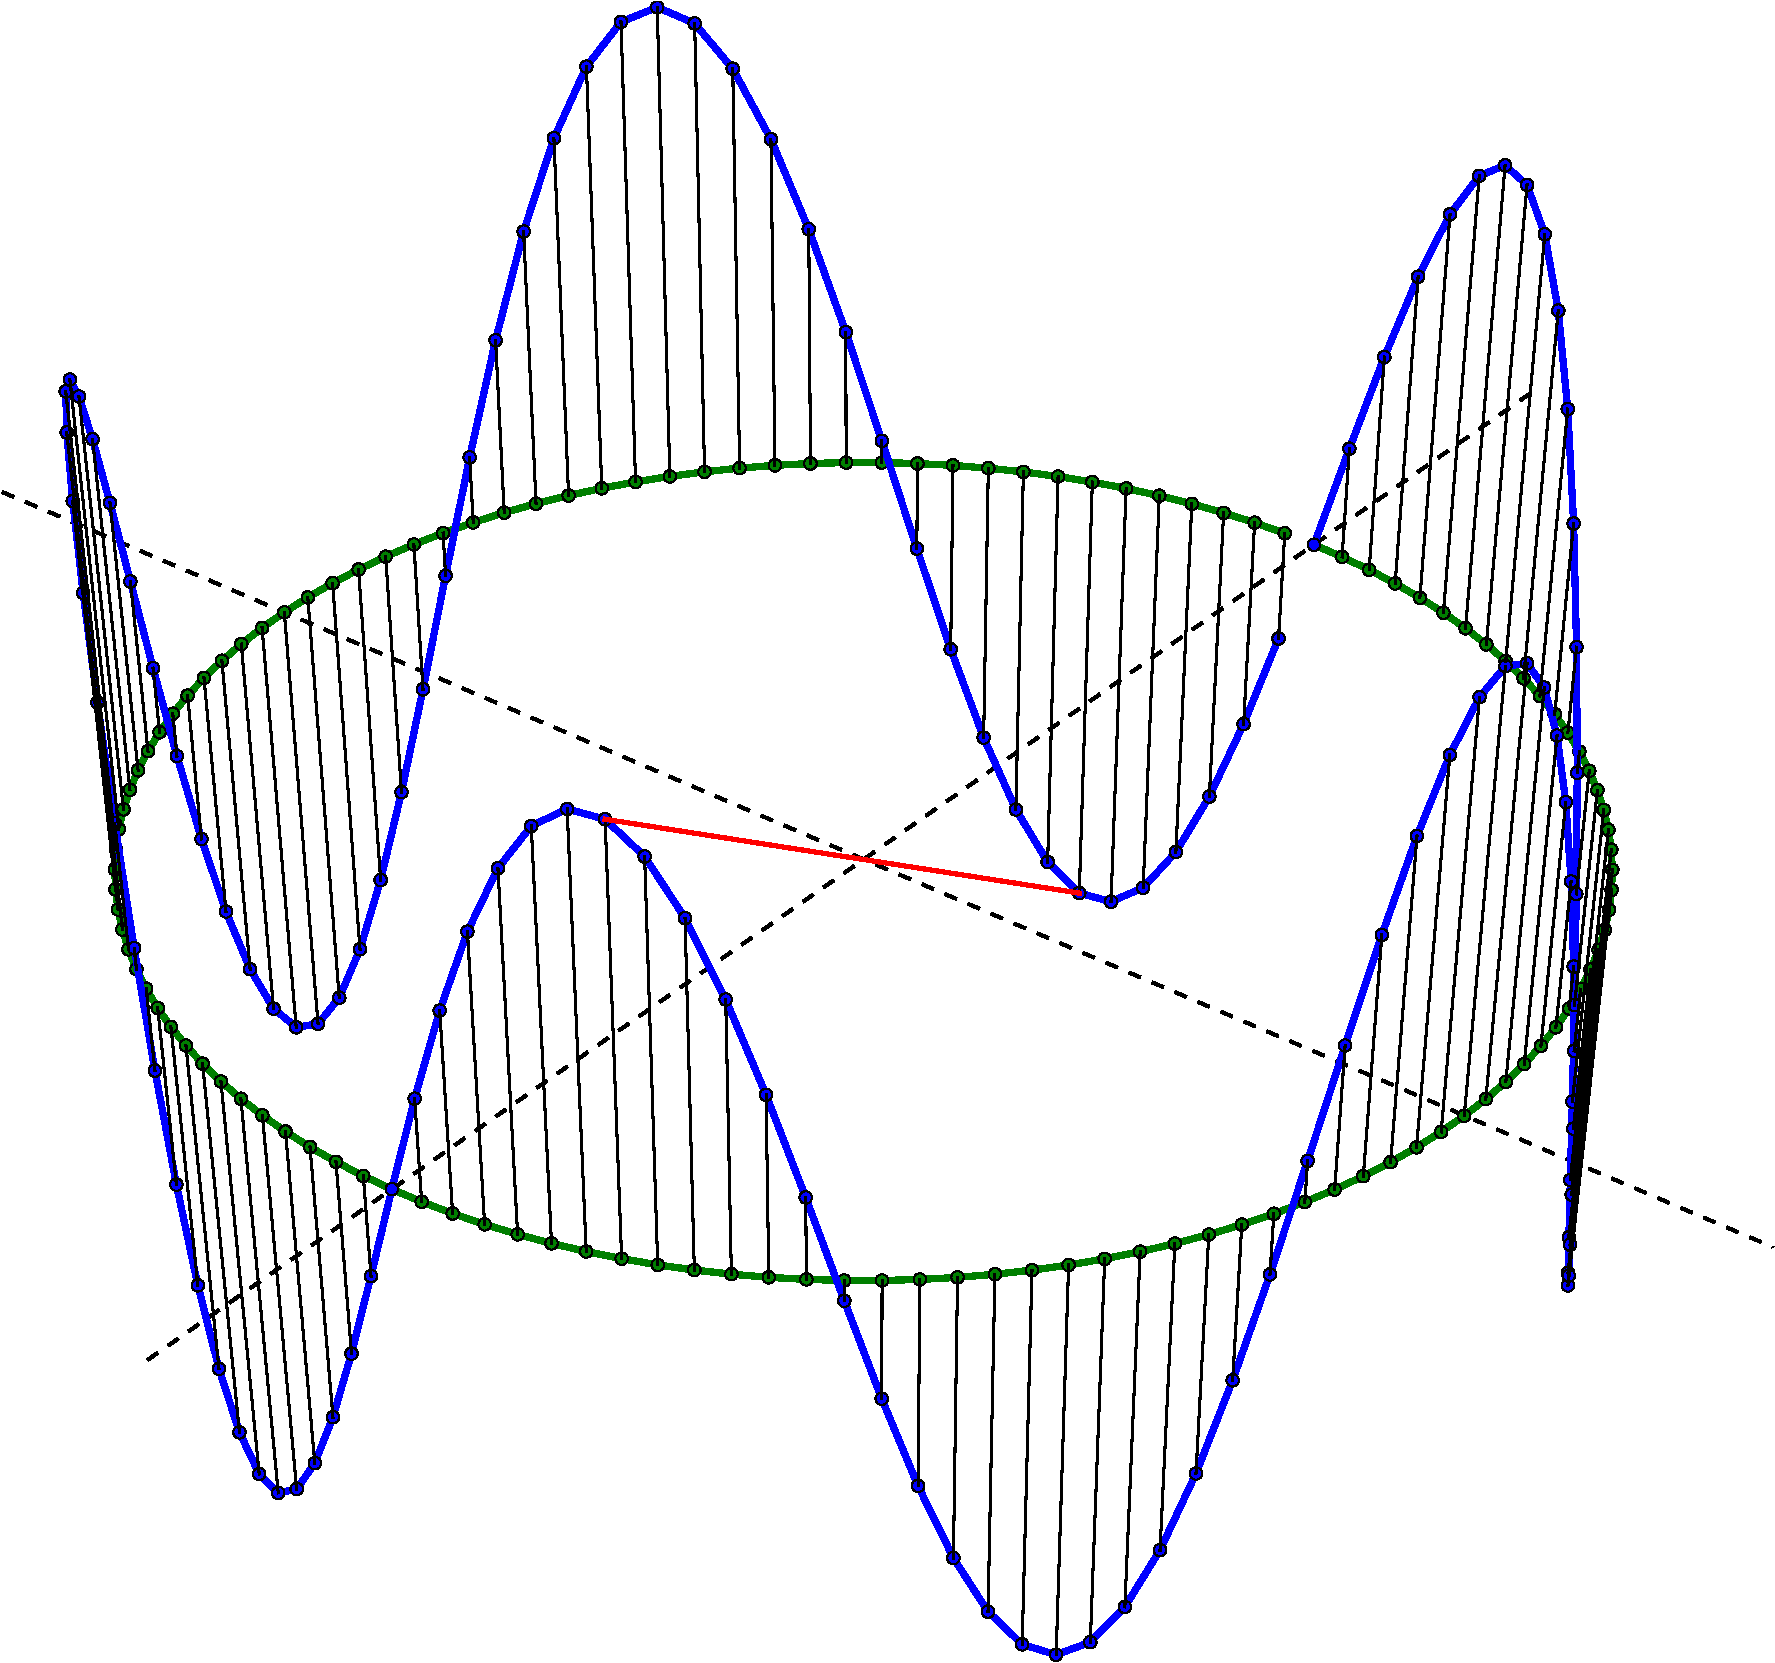
\includegraphics[width=0.8\textwidth]{fig/mode_5}
        \caption{An odd mode.}
    \end{subfigure}
        \caption{The point diametrically opposite for a mode located at radius $\rho$ has the same value as the point under consideration for an even mode, but the same value with a changed sign for even modes.
        The red soid line connects points diametrically opposite of each other.}
    \label{fig:BCLaplace}
\end{figure}

\section{Spectral filtering}
\label{sec:filt}
%
In order to ensure that no aliasing will occur and thereby create a numerical instability like the one mentioned in \cite{Phillips1959}, we must use a spectral filter in the periodic direction.
Although sufficiently high viscosities or diffusion can prevent aliasing (such that all the higher modes are damped out), they typically also damp modes which we would like to include in our simulation.
One way to get around this is to use spectral filters.

\subsection{Orszag's 2/3 rule}
As mentioned in \cite{Orszag1971}, only the $2/3$ of the topmost modes leads to aliasing.
To see this, recall that only mode numbers equal to or less than $N/2$ can be represented exactly on a grid discretized with $N$ points \cite{Bracewell2000book}.
Next, consider two mode numbers $m_1$ and $m_2$ which adds up to a mode $m_3$.
If $m_3=m_1+m_2>N/2$, the mode will be interpreted as $m_1+m_2 - N$ (i.e. it will be aliased to the negative frequencies).
If we call $M$ the highest mode we can have which would not give aliasing, we must require that
%
\begin{align*}
    m_1+m_2 - N &< -M\\
    M + M - N &< -M\\
    2M - N &< -M\\
    3M &<  N\\
    M &< \frac{N}{3}.
\end{align*}
%
In order words, modes with mode number less than $N/3$ does not contribute to aliasing.
Therefore, the name "$2/3$-rule" as $M$ is $2/3$ of the Nyquist frequency $M < (2/3)(N/2)$.

Thus, aliasing in this case is prevented if we set all modes with a mode number equal or above $N/3$ to zero.
As we see in the next section, this does not completely eliminate the aliasing in a cylinder, due to radial coupling.

\subsection{Radial coupling}
%
As terms like $\{\phi, f\}$ effectively advects modes of $f$ radially, we must ask ourselves what the smallest allowed wave length in the periodic direction is.
Since the circumference is given by $C=2\pi\rho$, and since the number of points in the periodic $\theta$-direction is constant, we see that resolution is limited by the shortest allowed wave length at the outermost radius $L_\rho$.
Let us now consider sinusoids on the form $\sin(kx)$ living on the circumference $C$ at radius $\rho$.
The wave number is then given by $k=\frac{2\pi m}{C}$, which means that the wavelength is
%
\begin{align}
    \lambda = \frac{C}{m}.
    \label{eq:wavelen}
\end{align}
%
The smallest resolved wavelength on $\rho=L_\rho$, where $L_\rho$ is the outermost radius, and is given by the Nyquist frequency.
This gives the wavelength $\lambda_{\text{Nyquist}} = \frac{C_{L_\rho}}{n_\theta/2}$, where $n_\theta$ is the number of points in the $\theta$ direction.
However, the smallest wavelength which does not give aliasing is given by the $2/3$-rule, so that
%
\begin{align*}
    \lambda_\min = \frac{C_{L_\rho}}{\frac{2}{3}\frac{n_\theta}{2}} = \frac{3C_{L_\rho}}{n_\theta}.
\end{align*}
%
By rearranging \cref{eq:wavelen}, we find that the largest allowed mode number for the circumference $C$ at radius $\rho$ is
%
\begin{align*}
    m_\max = \L\lfloor \frac{C}{\lambda_\min}\R\rfloor,
\end{align*}
%
where $\lfloor \cdot \rfloor$ denotes the floor function.
Note that we take the floor as we are looking for the maximum allowed integer.

\chapter{Verification of the numerics}
\label{chap:verification}
In the same sense that it is important to verify that the assumption in our
models are good, we need to ensure that the machinery handeling the numerical
calculation is correctly implemented.

Quoting \cite{Dudson2016}

\blockquote{
Code verification is a process of checking that the chosen set of partial
differential equations is solved correctly and consistently, and is a purely
mathematical exercise. Code verification is not concerned with verifying that
the chosen numerical methods are appropriate for the chosen set of equations.
Code verification is also not concerned with testing the ability of a given
model to explain experimental observations. This testing is dealt with in the
subsequent validation process.
}

Thus a code can be verified numerically, but still fail to match the desired
features of a real life experiment, and hence fail the validation process. If
the code has succuessfully passed a validation test, but fails a verification
test, the success of the validation is questionable, and the success of the
validation could be a mere coincident.
The verification process can be time consuming, and can almost be regarded as
an artform in itself. The process is throughly discussed in
\cite{Oberkampf2010book}, and more condensed for the method of manufactured
solution (MMS) in \cite{Salari}. The BOUT++ framework is verified using MMS in
\cite{Dudson2016}, presented briefly in section \ref{sec:MMS} after introducing
the concept of errors.

\section{Numerical errors}
Our derivative operators are discretized in order for them to operate on a discretized
grid. Doing so introduces an error, which depends on the order of
approximation. To use a concrete example, let us consider the simplest
differential equation
%
\begin{align}
    \deri{f(x)}{x} = g(x)
    \label{ver:ode}
\end{align}
%
where $f(x)$ and $g(x)$ are arbitrary functions (not to be confused with the
distribution function and a metric element). We seek to solve equation
(\ref{ver:ode}) for $f(x)$.

Let us find the simplest approximation of the derivate in an arbitrary grid
point $x_0$. We first Taylor expand $f(x)$ around $x_0$ (where $h$ is the grid
spacing) and evaluate it in $x_0 + h$, which gives
%
\begin{align*}
    f(x_0+h)
    = f(x_0)
    + h \L.\deri{f(x)}{x}\R|_{x=x_0}
    + \L.\frac{h^2}{2}\deri{^2f(x)}{x^2}\R|_{x=x_0}
    + \mathcal{O}(h^3)
\end{align*}
%
Subtraction of $f(x_0)$ and division by $h$ now yields the following
approximation of the derivative
%
\begin{align*}
    \frac{f(x_0+h) - f(x_0)}{h}
    =  \L.\deri{f(x)}{x}\R|_{x=x_0}
    + \L.\frac{h}{2}\deri{^2f(x)}{x^2}\R|_{x=x_0}
    + \mathcal{O}(h^2)
\end{align*}
%
Hence, the local truncation error LTE we do in a single point by using this
approximation is
%
\begin{align*}
    |e_{\text{LTE}}|
    =
    \L|\frac{f(x_0+h) - f(x_0)}{h} - \L.\deri{f(x)}{x}\R|_{x=x_0}\R|
    =
    \L| \L.\frac{h}{2}\deri{^2f(x)}{x^2}\R|_{x=x_0}
    + \mathcal{O}(h^2)\R|
\end{align*}
%
In other words it scales with the gridspacing $h$ to the first order.
The global error in some $L$-norm $n$ can be defined as
%
\begin{align*}
    \L\|\ve{e}\R\|_{L_n} =
    \L\|\ve{f}_{\text{true}} - \ve{f}_{\text{numeric}}\R\|_{L_n}
\end{align*}
%
% FIXME: LTE and global error
FIXME: LTE and global error
where $\ve{f}_{\text{true}}$ is an array of the analytic solution in each grid
point, and $\ve{f}_{\text{numeric}}$ is an array of the solution obtained
numerically. From linear PDE theory we have that the global error should
converge to the LTE order if the scheme is consitent (the LTE $\to 0$ as
$h\to 0$) and numerically stable%
\footnote{Note
that the deifintion of stability depends on the context, see
\cite{Leveque2007book} for more details.}.
%
If convergence is observed, the implementation is verified.

\section{MMS}
\label{sec:MMS}
For most PDEs, the true solution $\ve{f}_{\text{true}}$ is not known in
advance. Sometimes a solution can be found in some special limits.  If
convergence is found for these special cases, the code is not generally
verified, as there could still be implementation mistakes (not discoverable in
the limiting cases), but which could have dire consequences when a more general
solution is sougth numerically. One way to get around the problem is to
manufacture a solution.

Assume that we have a set of nonlinear spatiotemporal PDEs we would like to
solve for. Let us call the variables evolved in time for
$\ve{f}=\{\ve{u}_e, \ve{u}_i, n, \Om^D, T_e, \ldots\}$. If there are no mixed
spatial and temporal variables, we can write the set of nonlinear PDEs as
%
\begin{align}
  \parti{\ve{f}}{t} = F(\ve{f}) \RA \parti{\ve{f}}{t} - F(\ve{f}) = \ve{0}
  \label{ver:setOfPDE}
\end{align}
%
where $F(\cdot)$ is a nonlinear operator which contains the discretized spatial
differential operators. As stated above, we do not know apriori which $\ve{f}$
which satisfies equation (\ref{ver:setOfPDE}). Therefore we manufacture a
set of functions $\ve{f}_M$ which does not satisfy equation
(\ref{ver:setOfPDE}), but rather
%
\begin{align*}
    \parti{\ve{f}_M}{t} - F(\ve{f}_M) = \ve{S}
\end{align*}
%
Note that $\ve{f}_M$ is an exact analytical solution of $\parti{\ve{f}}{t} =
F(\ve{f}) + \ve{S}$. We can therefore solve numerically $\parti{\ve{f}}{t} =
F(\ve{f}) + \ve{S}$ for $\ve{f}$, and find the global error (for each variable
$\ve{u}_e, \ve{u}_i, n, \Om^D, T_e, \ldots$ by
%
\begin{align*}
    \L\|\ve{e}\R\|_{L_n} =
    \L\|\ve{f}_{M} - \ve{f}_{\text{numeric}}\R\|_{L_n}
\end{align*}
%
One can now test if the global error show the expected order of convergence.
Note that $\ve{f}_M$ and the coefficients in the various terms in the PDEs does
not need to be physical, but that in order to test all terms in this set of
equations, the parameters of the simulation should be chosen so that the
magnitude of each term is of a similar order of magnitude.


\section{MES}
%
There are, however, implementations in this thesis which is not covered by the
BOUT++ framework, and these should be verified as well. As these
implementations are single operations where an exact analytic solution can be
found, the approach to verify these has been through the method of exact
solutions (MES), i.e. there is no need to manufacture a solution. As with MMS,
there are several things to be aware of when performing MES, in particular when
dealing with cylinder geometry as there is an singularity at $\rho=0$. Calling
$f(\rho,\theta,z)$ for the function we are operating on with a discretized
operator $D$ (in such a way that $D[f(\rho,\theta,z)]=S$, where $S$ is the
result of the operation), the following criteria must be fullfilled for the
$f(\rho,\theta,z)$ under consideration
%
\vspace{0.5cm}
\begin{enumerate}[noitemsep,nolistsep]
    \item $f(\rho,\theta,z) = f(\rho,\theta+2\pi,z)$.
    \item $f(\rho,\theta,z)$ must be of $\mathcal{C}^\infty$, particularly at
    \begin{enumerate}[noitemsep,nolistsep]
        \item $f(\rho,\theta=0,z)$ and $f(\rho,\theta=2\pi,z)$.
        \item $f(\rho=0,\theta,z)$ (although the coordinates has a singularity
            there).
    \end{enumerate}
    \item $f(\rho, \theta, z)$ must be continuous in the $\rho$ direction with
          $f(\rho, \theta + \pi, z)$.
  \item Boundary conditions in $\rho$ and $z$ must be satisfied.
\end{enumerate}
%
A function which satifies the above is
%
\begin{align*}
    f(\rho, \theta, z)
    =& \sin\L(
        \frac{1}{\sqrt{2}}\rho[\cos(\theta)+\sin(\theta)]\frac{2\pi}{2L_\rho}
          \R)
      \\&
      \exp\L(
        -\frac{1}{2w^2}
            \L[\rho^2 + \rho_0^2 - 2\rho\rho_0(\cos[\theta - \theta_0])\R]
          \R)
      \\&
        \L(\frac{\rho\cos[\theta]+L_\rho}{2L_\rho}\R)^2
        \numberthis
        \label{eqapp:MESf1}
\end{align*}
%
where
%
\begin{align*}
    &L_\rho = 30&
    &\text{
        Cylinder radius
    }&
    \\
    &w = \frac{4}{5}L_\rho&
    &\text{
        Width of gaussian
    }&
    \\
    &\rho_0 = \frac{3}{10}L_\rho&
    &
    \rho
    \text{
        - coordinate for center of gaussian
    }&
    \\
    &\theta_0 = \frac{5\pi}{4}&
    &
    \theta
    \text{
        - coordinate for center of gaussian
    }&
\end{align*}
%
Equation \ref{eqapp:MESf1} will be function used in the discussion below if
nothing else is mentioned.
%
\begin{figure}[t!]
    \centering
    \begin{subfigure}[t]{0.45\textwidth}
        \centering
        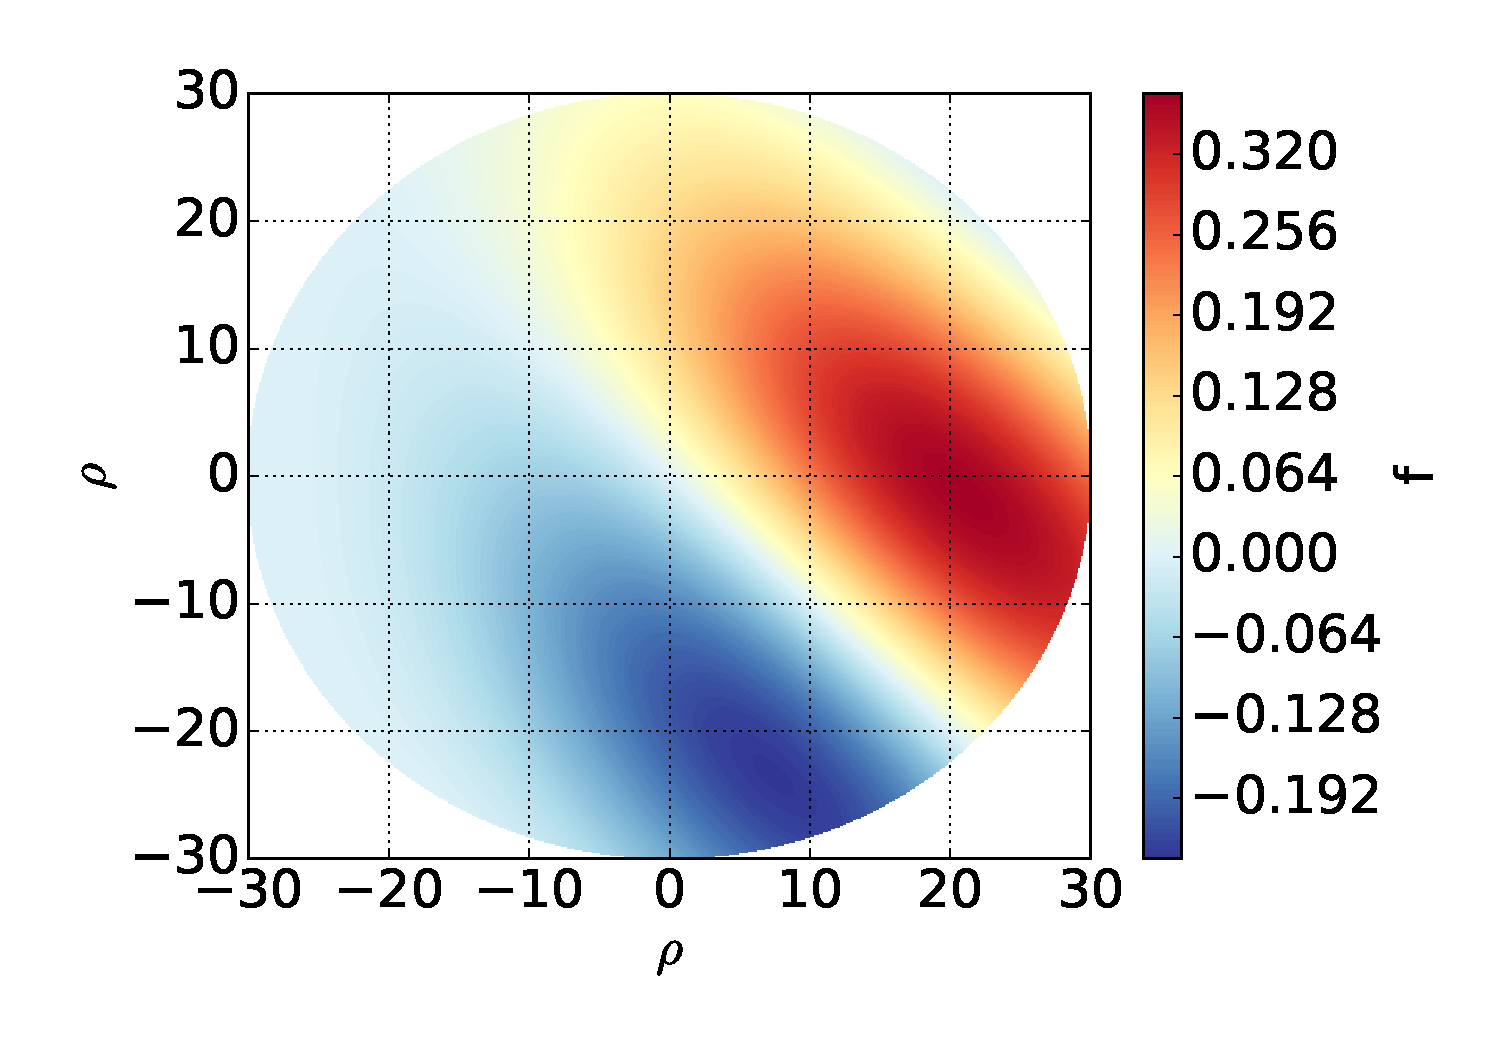
\includegraphics[width=1.0\textwidth]{fig/f}
        \caption{The function used in the MES}
    \end{subfigure}%
    ~
    \begin{subfigure}[t]{0.45\textwidth}
        \centering
        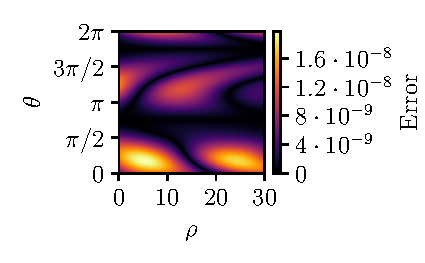
\includegraphics[width=1.0\textwidth]{fig/err}
        \caption{Typical plot of the errors}
    \end{subfigure}
    ~
    \begin{subfigure}[t]{0.45\textwidth}
        \centering
        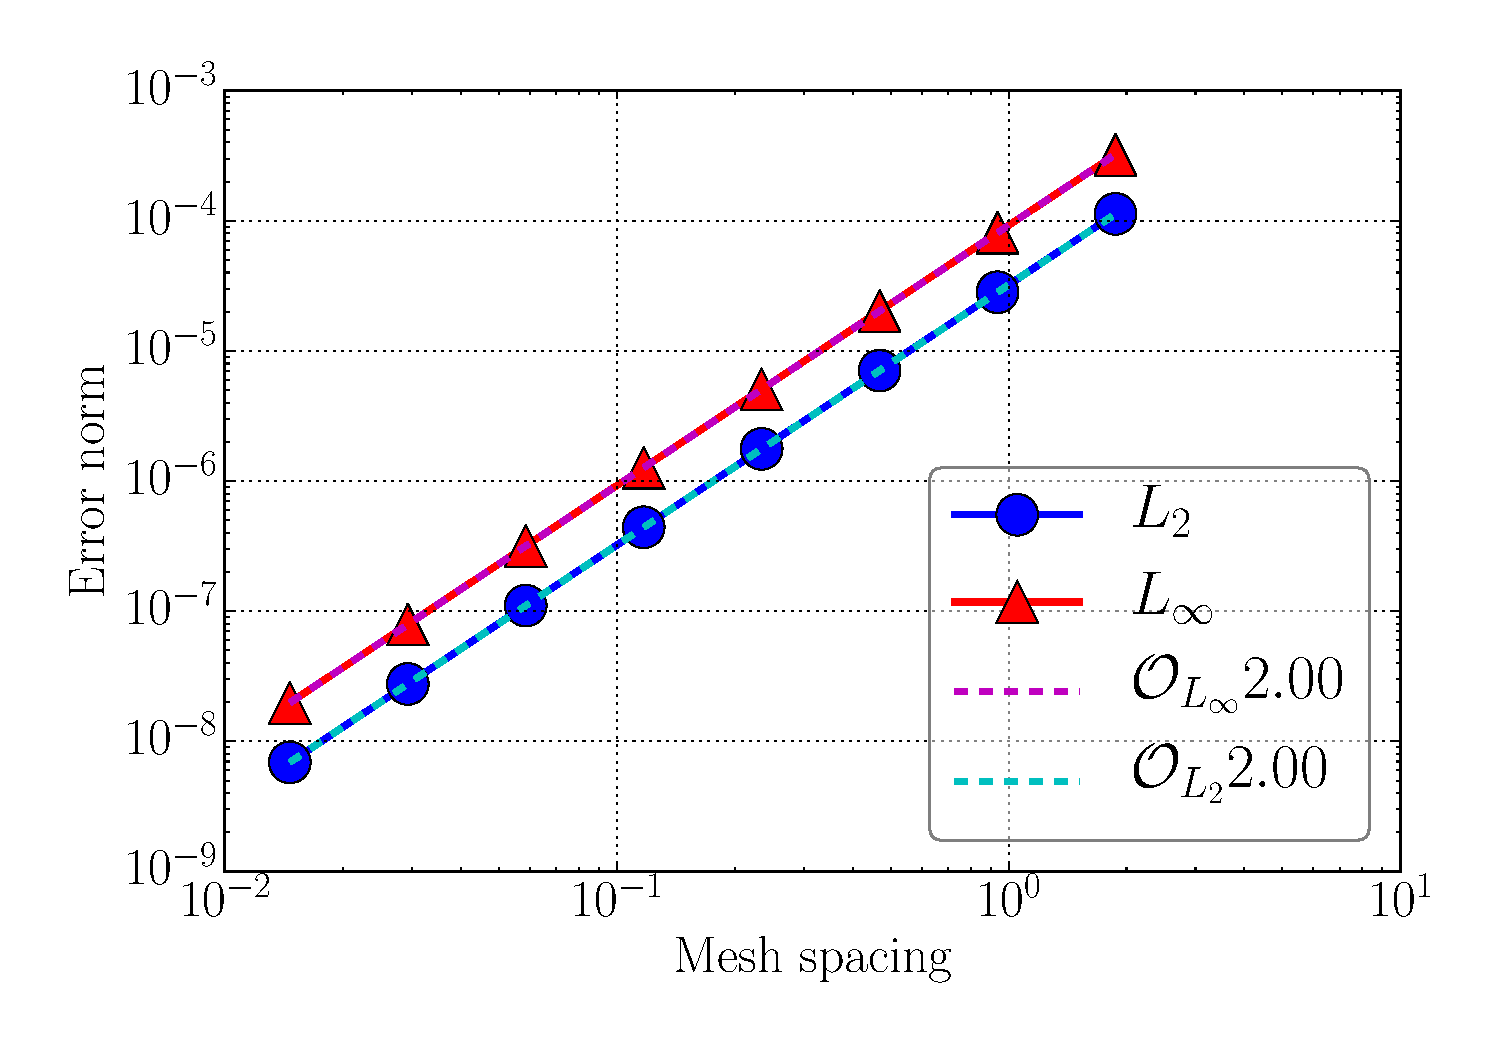
\includegraphics[width=1.0\textwidth]{fig/conv}
        \caption{Typical convergence plot}
    \end{subfigure}
    \caption{Typical function and errors for MES}
\end{figure}

\subsection{Single operators}
%
Although the single operators available from BOUT++ is verified in
\cite{Dudson2016}, the axis of a cylinder must be treated with care as there is
a singularity there ($J=0$ at $\rho=0$). To overcome this problem the
solution described in \cite{Naulin2008} has been used, and is illustrated in
figure \ref{fig:innerRho}.
%
\begin{figure}[htb]
    \centering
    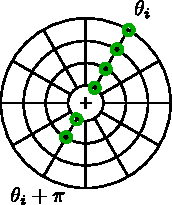
\includegraphics[width=0.3\textwidth]{fig/innerGhost}
    \caption{\textit{
        The green full circles represents the inner grid points at
        $\theta=\theta_i$. The green dashed circles at $\theta=\theta_i + \pi$
        are the ghost points (in the $\rho$-direction) belonging to the
        $\theta=\theta_i$ inner points. Equally the inner grid points at
        $\theta=\theta_i$ serves as ghost points (in the $\rho$-direction) for
        the inner points of $\theta=\theta_i + \pi$.
    }}
    \label{fig:innerRho}
\end{figure}
%
In this solution, the
the innermost ghost points%
\footnote{A grid point not belonging to the physical domain, but makes it
    possible to use a centered scheme when evaluating at the grid point closest
    to the physical boundary of the domain.}
in $\rho$ (closest to the singularity) with a
$\theta$ value lower
than (and excluding) $\pi$ will be set to the value of the innermost
internal point%
\footnote{A grid point which is not a ghost points, i.e. it belongs to the
    physical domain.}%
%
which lies
$\theta + \pi$ away. The next ghost point will be set to the value of the
second innermost internal point which lies $\theta + \pi$ away, and so on. In
this thesis, only one ghost point is used.

The convergence test for the single operators in $\rho$ direction can be found
in table \ref{tb:singleRho}.
%
\begin{table}[h!]
{\footnotesize \centerline{
\begin{tabular}{c|llllp{3cm}}
\hline\hline
Operation & $L_\inf$ order & $L_2$ order &
$L_\inf$ error ($2^{12}$ points) & $L_2$ error ($2^{12}$ points) & Comment\\
\hline
$\texttt{DDX}  (f)$ & $2.00$ & $2.00$ & $1.99\cdot10^{-8}$ & $6.90\cdot10^{-9}$& \\
$\texttt{D2DX2}(f)$ & $2.00$ & $2.00$ & $1.58\cdot10^{-9}$ & $5.07\cdot10^{-10}$& \\
$\texttt{D3DX3}(f)$ & $1.73$ & $2.00$ & $9.66\cdot10^{-10}$ & $1.57\cdot10^{-9}$&
$L_\inf$ order $=2$ until $2^{11}$ points
\\
$\texttt{D2DXDZ} (f)$ & $2.00$ & $2.00$ & $1.09\cdot10^{-8}$ & $2.97\cdot10^{-8}$& \\
$\texttt{D3DX2DZ}(f)$ & $2.00$ & $1.94$ & $2.33\cdot10^{-9}$ & $8.51\cdot10^{-10}$&
$L_\inf$ order $=2$ until $2^{11}$ points
\\
$\texttt{D3DZ2DX}(f)$ & $2.00$ & $2.00$ & $7.68\cdot10^{-8}$ & $2.88\cdot10^{-8}$& \\
$\texttt{DDX}   (Jf)$ & $2.00$ & $2.00$ & $5.22\cdot10^{-7}$ & $1.71\cdot10^{-7}$& \\
$\texttt{DDX}(\texttt{DDX}[f])$ & $-1.00$ & $-0.50$ & $1.67\cdot10^{0}$ & $2.60\cdot10^{-2}$&
Solution diverges. Errors dominating close to $\rho=0$.
\\
$\frac{\texttt{DDX}(f)}{J}$ & $1.00$ & $1.50$ & $3.16\cdot10^{-5}$ & $4.48\cdot10^{-7}$&
No order $2$nd order convergence. Errors dominating close to $\rho=0$.
\\
\hline\hline
\end{tabular}
}}
\caption[]{\textit{Convergence test of single operators in the $\rho$ direction}}
\protect\label{tb:singleRho}
\end{table}
%
For the cases where a convergence order of $2$ is found up until $2^{11}$
points, the schemes are considered convergent as the error is not dominating at
any particular point of the domain. In general, one can observe from the plots
of the error that they become a bit noisy in these cases, which could indicate
that machine precision in reached.

Note in the two last cases in table \ref{tb:singleRho} that the converge one
naively would have expected is generally not reached. In the case where we use
$\texttt{DDX}(\texttt{DDX}[f])$, the boundaries are reset after the first
operation. Notice that the resulting of stencil of these two operators is a
wide stencil. That is
%
\begin{align*}
D[D[f_i]] =& D\L[\frac{-f_{i-1} + f_{i+1}}{h_x}\R]
\\
=& \frac{-D[f_{i-1}] + D[f_{i+1}]}{h_x}
\\
=& \frac{-\frac{-f_{i-2} + f_{i}}{h_x} + \frac{-f_{i} + f_{i+2}}{h_x}}{h_x}
\\
=& \frac{f_{i-2} - 2f_{i} + f_{i+2}}{h_x^2}
\end{align*}
%
where $h_x$ denotes the grid spacing, and the subscript the grid index. Hence,
the observed divergence could be explained with poor information communication
across the singularity.

In the case of $\frac{\texttt{DDX}(f)}{J}$, the loss of expected convergence
rate can be explained by looking at the operator under investigation. As the
$\texttt{DDX}(f)$ operator used in this thesis is the standard $2$nd order
operator (obtained by subtracing the function Taylor expanded around $x_0$,
evaluated in $x+h$ from the function Taylor expanded around $x_0$,
evaluated in $x-h$ and divided by $2h$), one find that
%
\begin{align*}
    \deri{f}{x} - \texttt{DDX}(f) =
    \frac{h^2}{6}\deri{^2f}{x^2} + \mathcal{O}(h^3)
\end{align*}
%
In the first inner point $J=h_x$ as the boundaries lays half between the grid
points. Thus, in this point, we have that
%
\begin{align*}
    \frac{ \L.\deri{f}{x} \R|_{\text{first} \rho}}{J}
    - \frac{\L. \texttt{DDX}(f)\R|_{\text{first} \rho}}{J}=
    \frac{h}{6}\deri{^2f}{x^2} + \mathcal{O}(h^2)
\end{align*}
%
Thus for the first inner point, the scheme is not $2$nd order convergent.

Only one extra operator is implemented in the $\theta$-direction. This is shown
in table \ref{tb:singleZ}. Note that we use spectral methods in the $\theta$
direction, which is know to give minimal error. Machine precision is therefore
quickly reached, and performing MES after machine precision is nonsense due to
loss of percision when subtracting two amlost equal numbers. Indications that
machine precision is reached are low errors, and plots of the error appearing
noisy
%
\begin{table}[h!]
{\footnotesize \centerline{
\begin{tabular}{c|llllp{3cm}}
\hline\hline
Operation & $L_\inf$ order & $L_2$ order &
$L_\inf$ error ($2^{6}$ points) & $L_2$ error ($2^{6}$ points) & Comment\\
\hline
\texttt{D3DZ3}$(f)$ & $2.06$ & $2.10$ & $7.44\cdot10^{-11}$ & $7.33\cdot10^{-12}$&
Reaches machine precision at $2^6$.
\\
\hline\hline
\end{tabular}
}}
\caption[]{\textit{Convergence test single operators in the $\theta$ direction.}}
\protect\label{tb:singleZ}
\end{table}



\subsection{Divergence operators}
%           ▸ 1a-divPerp/
%           ▸ 1b-JTimesDivPerp/
%           ▸ 2a-divSource/
%           ▸ 2b-JTimesDivSource/
%           ▸ 3a-divExBAdv/
%           ▸ 3b-J4divExBAdv/

\subsection{The Naulin Solver}
% FIXME: Write about the function
functions here
mention BC
write implementation somewhere
\begin{table}[h!]
{\footnotesize \centerline{
        \begin{tabular}{lllll}
\hline\hline
$L_\inf$ order & $L_2$ order &
$L_\inf$ error ($2^{12}$ points) & $L_2$ error ($2^{12}$ points)\\
\hline
$2.00$ & $2.00$ & $3.19\cdot10^{-7}$ & $1.65\cdot10^{-7}$\\
\hline\hline
\end{tabular}
}}
\caption[]{\textit{Convergence test of the Naulin Solver in the $\rho$ direction}}
\protect\label{tb:naulinSolver}
\end{table}
%          ▸ Naulinsolver0Bndry/

\subsection{Boundary conditions}
%          ▸ 1-yExtrapolation/
%          ▸ 2-uEParSheath/
%          ▸ 3-cauchyBC/


\part{Results}
\label{part:results}
We will in this part discuss the findings of the simulations of the CELMA code.
Hang tight, the results will come soon, current draft
%
\begin{itemize}[noitemsep]
    \item Growth rates (extended) vs slab
    \item Steady state vs averaged profile
    \item Profiles subplot of three
    \begin{itemize}[noitemsep]
        \item Gradient in $n$
        \item $n$ fluct
        \item $\phi$ fluct
    \end{itemize}
    \item Energy shows predator-prey
    \item Scan $B_0$
    \item Scan $n_n$
    \item Compare everything with Boussinesq
\end{itemize}
%
additional
%
\begin{itemize}[noitemsep]
    \item Probe signals
    \begin{itemize}[noitemsep]
        \item Mode
        \item $n$ fluct
        \item $\phi$ fluct
        \item Flux
        \item PDF
        \item SPD, $1$D and $2$D
    \end{itemize}
\end{itemize}
%
Could check
%
\begin{itemize}[noitemsep]
    \item Shear flow
    \item Streamers
    \item Blobs
    \item Energy limit cycle if still exsists
    \item Kinetic and potential energy predator prey if still exsits
\end{itemize}
%
% FIXME: Insert the results here


\part{Appendices}
\appendix
\chapter{Drift ordering}
\label{app:DO}
We will in this section look at big and small terms in the perpendicular momentum equation in \cref{eq:perp_mom_start}.
The motivation for this is to make a drift ordering similar to what is done in \cite{Fitzpatrick2014book} and from this get algebraic equations for each order of the perpendicular velocities.
We will do so by looking at characteristic scales of the system.
Before starting, we will have a brief look at the definition of the gradient length scales and of the quasi-neutrality of the system.

\section{Gradient length scale}
We will here do order of magnitude estimates%
\footnote{
    Easy, approximate ways to estimate some numbers within the same orders of magnitudes as we would have reached by doing a more correct and rigorous study.
}%
, and will therefore introduce the \emph{gradient length scale}.
The gradient scale length serves as an estimate for the size of $\grad$.
That is, it tells us over how large distances there are sharp gradients for a bounded, smooth function.
For a field $f$, the gradient length scale $L_f$ is defined as%
\footnote{
    Note that the inverse gradient length scale is often denoted $k$ in the literature.
    This make sense plane wave perturbations, which happens to have $\frac{1}{L_f}=k$, where $k$ is the inverse wave number.
    However, in order to avoid ambiguity, we will in this thesis use $L_f$ for the gradient scale length.
}%
%
\begin{align}
    \frac{1}{L_f} \defined \frac{\|\max\{\operatorname{abs}(\grad f)\}\|}{\operatorname{abs}\L(f\bigg|_{\|\max\{\operatorname{abs}(\grad f)\}\|}\R)},
    \label{eq:lenScale}
\end{align}
%
i.e. short and sharp gradients in $f$ have a short $L_f$.
We can similarly define the temporal scale as
%
\begin{align}
    \om_f = \frac{1}{\tau_f} \defined \frac{\max\{\operatorname{abs}(\partial_t f)\}}{\operatorname{abs}\L(f\bigg|_{\max\{\operatorname{abs}(\partial_t f)\}}\R)}.
    \label{eq:timeScale}
\end{align}
%
The definitions in \cref{eq:lenScale,eq:timeScale} are quite strict, and we will in this thesis use a more approximate estimate for the gradient length scale.
Thus, when referring to gradient length scales in this thesis, we will mean "typical" values for the gradient scale lengths, so that
%
\begin{align*}
    \grad \sim \frac{1}{L},
\end{align*}
%
where $\sim$ denotes "of same order".

\section{Quasi-neutrality}
\label{sec:qn}
To get the condition of whether the system is quasi-neutral or not, we can do an order of magnitude estimate comparison of $Zn_i$ and $Zn_i - n_e$.
We find that
%
\begin{align}
    \frac{Zn_i - n_e}{Zn_i} =
    \frac{e(Zn_i - n_e)}{eZn_i}
    =
    \frac{\e_0\div\ve{E}}{eZn_i}
    \sim
    \frac{\e_0\L|E\R|}{\L|L_E\R|eZn_i}.
    \label{eq:quasiNeutral}
\end{align}
%
We can find an approximate expression for $E$ through Faraday's induction law:
%
\begin{align*}
    \curl\ve{E} =& -\partial_t B\\
    \frac{|E|}{|L_E|} \sim& \frac{|B|}{\tau_B}\\
    |E| \sim& \frac{|L_E||B|}{\tau_B}.
\end{align*}
%
Inserting this in \cref{eq:quasiNeutral} yields
%
\begin{align*}
    \frac{Zn_i - n_e}{Zn_i}
    \sim
    \frac{\e_0 |L_E||B|}{|L_E| e Zn_i \tau_B}\frac{m_i Ze}{m_i Ze}
    =
    \frac{\om_{ci}\e_0}{Z e n_i\tau_B}\frac{m_i}{Z e}
    =
    \frac{\om_{ci}}{\tau_B\om_{pi}^2},
\end{align*}
%
where $\om_{pi}$ denotes the ion plasma frequency%
\footnote{This can be interpreted as something like the typical frequency the ions would oscillate with if the ions where perturbed in a completely quiescent plasma.}
%
.
We will now assume that the fastest time scales which can occur in our system is much slower than the ion cyclotron frequency.
If we therefore set $1/\tau_B\to\om_{ci}$, we get
%
\begin{align}
    \frac{Zn_i - n_e}{Zn_i}
    \simeq
    \frac{\om_{ci}^2}{\om_{pi}^2}
    =
    \frac{\om_{ci}^2}{\om_{pi}^2},
    \label{eq:quasiNCompare}
\end{align}
%
which for our interest is a quantity much smaller than $1$.

Equivalently, if we introduce the \emph{normalizing} ion sound speed%
%
\footnote{Although the real ion sound speed is given by $c_s=\sqrt{\frac{T_e+\gamma' T_i}{m_i}}\;\gamma'=\frac{N+2}{N}$ for $N$ degrees of freedom, we will in this thesis use the symbol $c_s$ for $\sqrt{\frac{T_e}{m_i}}$, as this term frequently pops up in the derivations.}
%
\begin{align*}
    c_s = \sqrt{\frac{T_e}{m_i}},
\end  {align*}
%
and the ion hybrid radius (the ion gyro radius at the electron temperature)
%
\begin{align*}
    \rho_s=\frac{c_s}{\om_{ci}}.
\end  {align*}
%
\Cref{eq:quasiNCompare} can be stated as
%
\begin{align*}
    \frac{Zn_i - n_e}{Zn_i}
    \simeq
    \frac{\om_{ci}^2}{\om_{pi}^2}
    =
    \frac{c_s^2\om_{ci}^2}{c_s^2\om_{pi}^2}
    =
    \frac{c_s^2}{\rho_s^2\om_{pi}^2}
    =
    \frac{\frac{T_e}{m_i}}{\rho_s^2\frac{n_iZ^2e^2}{m_i\e_0}}
    =
    \frac{\frac{T_e\e_0}{n_iZ^2e^2}}{\rho_s^2}
    =
    \frac{\lambda_D^2}{\rho_s^2},
\end{align*}
%
where $\lambda_D$ is the Debye length, which tells at what distance an isolated charge is effectively electrically shielded by surrounding charged particles.

In other words, the quasi-neutrality is just a statement of what scales we are looking at.
Note that this does not imply that there cannot be large electrical field throughout the plasma, rather that the left hand side of
%
\begin{align*}
    \frac{\div \ve{E}}{Zn_i} = \frac{e}{\e_0} \frac{Zn_i-n_e}{Zn_i}
\end{align*}
%
is small (as $e$ and $\e_0$ is of the same order of magnitude).
We therefore have
%
\begin{align*}
    n\simeq Zn_i \simeq n_e.
\end{align*}

\section{The inertia term}
\label{sec:doInert}
The left hand side of \cref{eq:perp_mom_start} reads
%
\begin{align*}
&
 \frac{1}{\om_{c\a}}
 \L(
 \partial_t \ve{u}_{\a,\perp}
 + \L[\ve{u}_{\a,\perp}
 + \ve{u}_{\a,\|}\R]\cdot\grad\ve{u}_{\a,\perp}
 \R)
\\
 %
 %
 %
 =&
 \frac{1}{\om_{c\a}}
 \L(
 \partial_t \ve{u}_{\a,\perp}
 + \L[\ve{u}_{\a,\perp}
 + \ve{u}_{\a,\|}\R]\cdot\grad\ve{u}_{\a,\perp}
 \R)
 \\
 %
 %
 %
 =&
 \frac{1}{\om_{c\a}}
 \L(
 \partial_t \ve{u}_{\a,\perp}
 + \ve{u}_{\a,\perp}\cdot\grad_\perp\ve{u}_{\a,\perp}
 + \ve{u}_{\a,\|}\cdot\grad_\|\ve{u}_{\a,\perp}
 \R).
 \numberthis
 \label{eq:do_inertia}
\end{align*}
%
From this, we can extract a characteristic timescale of change of the perpendicular velocity, a characteristic gradient length scale and a characteristic perpendicular velocity.
We will use the notation for a field $f$
%
\begin{align*}
    f = f^c \breve{f},
\end{align*}
%
where the superscript $f^c$ denotes the characteristic size of $f$ so that $\breve{f}$ is of $\mathcal{O}(1)$.
If we now apply this on \cref{eq:do_inertia}, we get
%
\begin{align*}
    &
 \frac{1}{\om_{c\a}}
 \L(
 \om^c_{\a,\perp}u^c_{\a,\perp}
 \partial_{\breve{t}} \breve{\ve{u}}_{\a,\perp}
 + \frac{u_{\a,\perp}^{c}u_{\a,\perp}^{c}}{L_{\perp, u_{\a,\perp}}}
 \breve{\ve{u}}_{\a,\perp}\cdot\breve{\grad}_\perp\breve{\ve{u}}_{\a,\perp}
 + \frac{u^c_{\a,\perp}u^c_{\a,\|}}{L_{\|, u_{\a,\perp}}}
 \breve{\ve{u}}_{\a,\|}\cdot\breve{\grad}_\|\breve{\ve{u}}_{\a,\perp}
 \R)
 \\
 %
 %
 %
 =&
 \frac{u^c_{\a,\perp}}{\om_{c\a}}
 \L(
 \om^c_{\a,\perp}
 \partial_{\breve{t}} \breve{\ve{u}}_{\a,\perp}
 + \frac{u^c_{\a,\perp}}{L_{\perp, u_{\a,\perp}}}
 \breve{\ve{u}}_{\a,\perp}\cdot\breve{\grad}_\perp\breve{\ve{u}}_{\a,\perp}
 + \frac{u^c_{\a,\|}}{L_{\|, u_{\a,\perp}}}
 \breve{\ve{u}}_{\a,\|}\cdot\breve{\grad}_\|\breve{\ve{u}}_{\a,\perp}
 \R).
\end{align*}
%
We now relate the velocities to $c_s$, so that
%
\begin{align*}
    \lambda \defined \frac{u^c}{c^c_s}.
\end{align*}
%
Further, by using the ion hybrid radius, we get
%
\begin{align*}
    &
 \lambda_{u_{\a,\perp}}
 \frac{c^c_s}{\om_{c\a}}
 \L(
 \om^c_{\a,\perp}
 \partial_{\breve{t}} \breve{\ve{u}}_{\a,\perp}
 +
 \lambda_{u_{\a,\perp}}
 \frac{ c^c_s }{L_{\perp, u_{\a,\perp}}}
 \breve{\ve{u}}_{\a,\perp}\cdot\breve{\grad}_\perp\breve{\ve{u}}_{\a,\perp}
 +
 \lambda_{u_{\a,\|}}
 \frac{L_{\perp, u_{\a,\perp}}}{L_{\perp, u_{\a,\perp}}}
 \frac{c^c_s}{L_{\|, u_{\a,\perp}}}
 \breve{\ve{u}}_{\a,\|}\cdot\breve{\grad}_\|\breve{\ve{u}}_{\a,\perp}
 \R)
 \\
 %
 %
 %
 =&
 \lambda_{u_{\a,\perp}}
 \frac{c^c_s}{\om_{c\a}}
 \L(
 \om^c_{\a,\perp}
 \partial_{\breve{t}} \breve{\ve{u}}_{\a,\perp}
 +
 \lambda_{u_{\a,\perp}}
 \frac{ \rho^c_s }{L_{\perp, u_{\a,\perp}}}
 \om^c_{ci}
 \breve{\ve{u}}_{\a,\perp}\cdot\breve{\grad}_\perp\breve{\ve{u}}_{\a,\perp}
 +
 \lambda_{u_{\a,\|}}
 \frac{L_{\perp, u_{\a,\perp}}}{L_{\|, u_{\a,\perp}}}
 \frac{\rho^c_s}{L_{\perp, u_{\a,\perp}}}
 \om^c_{ci}
 \breve{\ve{u}}_{\a,\|}\cdot\breve{\grad}_\|\breve{\ve{u}}_{\a,\perp}
 \R).
\end{align*}
%
We will now assume that the scales for the ions and electrons are the same.
This is, we are constraining the system in the following way
%
\begin{align*}
    \lambda              &\sim \lambda_{u_{e,\perp}}  \sim \lambda_{u_{i,\perp}} \\
    \om^c                &\sim \om^c_{e,\perp}        \sim \om^c_{i,\perp}       \\
    L_{\perp, u_{\perp}} &\sim L_{\perp, u_{e,\perp}} \sim L_{\perp, u_{i,\perp}}\\
    L_{\|, u_{\perp}}    &\sim L_{\|, u_{e,\perp}}    \sim L_{\|, u_{i,\perp}}.
\end{align*}
%
If we at the same time introduce
%
\begin{align*}
    \frac{ \rho^c_s }{L_{\perp, u_{\perp}}} \defined \gamma,
\end{align*}
%
we get
%
\begin{align}
 \lambda
 \frac{c^c_s}{\om_{c\a}}
 \L(
 \om^c
 \partial_{\breve{t}} \breve{\ve{u}}_{\a,\perp}
 +
 \lambda
 \gamma
 \om^c_{ci}
 \breve{\ve{u}}_{\a,\perp}\cdot\breve{\grad}_\perp\breve{\ve{u}}_{\a,\perp}
 +
 \lambda_{u_{\a,\|}}
 \frac{L_{\perp, u_{\a,\perp}}}{L_{\|, u_{\a,\perp}}}
 \gamma
 \om^c_{ci}
 \breve{\ve{u}}_{\a,\|}\cdot\breve{\grad}_\|\breve{\ve{u}}_{\a,\perp}
 \R).
 \label{eq:doLHSAfterFirstConstraint}
\end{align}
%
In order for these terms to  be of the same order, we must have that
%
\begin{align*}
 \om^c                    &\sim \lambda \gamma \om^c_{ci}  \sim \lambda_{u_{\a,\|}} \frac{L_{\perp}}{L_{\|, u_{\perp}}} \gamma \om^c_{ci}
 \\
 \frac{\om^c}{\om^c_{ci}} &\sim \lambda \gamma             \sim \lambda_{u_{\a,\|}} \frac{L_{\perp}}{L_{\|, u_{\perp}}} \gamma.
 \numberthis
 \label{eq:firstOrdering}
\end{align*}
%
If we assume low frequency turbulence, we must have that
%
\begin{align*}
    \frac{\om^c}{\om^c_{ci}} \defined \e \ll 1.
\end{align*}
%
Comparing the two first terms in \cref{eq:firstOrdering} gives
%
\begin{align*}
 \frac{\om^c}{\om^c_{ci}}
 \sim&
 \lambda
 \gamma
 \\
 \e
 \sim&
 \lambda
 \gamma
\end{align*}
%
in order to have a balanced restriction between gradient scale lengths and velocities.
We can set
%
\begin{align*}
 \lambda
 \sim&
 \sqrt{\e}
 \\
 \gamma
 \sim&
 \sqrt{\e}.
\end{align*}
%
Note that if we had started our constraint by saying $\sqrt{\e}\ll 1$ instead, the non-linear terms would be negligible.

Finally, we put the restriction on the parallel velocity and scale lengths.
We now define
%
\begin{align*}
\frac{L_{\perp}}{L_{\|, u_{\a,\perp}}}\defined \zeta.
\end{align*}
%
By assuming $u^c_{\a,\|}\sim c^c_s$, and that
%
\begin{align*}
\zeta\sim \sqrt{\e},
\end{align*}
%
we find that
%
\begin{align*}
 \lambda_{u_{\a,\|}}
 \frac{L_{\perp}}{L_{\|, u_{\a,\perp}}}
 \gamma
 =
 \lambda_{u_{\a,\|}}
 \zeta
 \gamma
 \sim
 1\sqrt{\e}^2
 =
 \e.
\end{align*}
%
This means that the left hand side of \cref{eq:perp_mom_start} can in an order of magnitude estimate be written as (assuming that $\om_{c\a}\sim\om^c_{c\a}$
%
\begin{align*}
 &
 \lambda
 \frac{m_i}{m_i}
 \frac{c^c_s}{\om^c_{c\a}}
 \L(
 \om^c
 \partial_{\breve{t}} \breve{\ve{u}}_{\a,\perp}
 +
 \lambda
 \gamma
 \om^c_{ci}
 \breve{\ve{u}}_{\a,\perp}\cdot\breve{\grad}_\perp\breve{\ve{u}}_{\a,\perp}
 +
 \lambda_{u_{\a,\|}} \frac{L_{\perp, u_{\a,\perp}}}{L_{\|, u_{\a,\perp}}}
 \gamma
 \om^c_{ci}
 \breve{\ve{u}}_{\a,\|}\cdot\breve{\grad}_\|\breve{\ve{u}}_{\a,\perp}
 \R)
 \\
 %
 %
 &=
 \lambda
 \frac{m_\a}{m_i}
 \frac{c^c_s}{\om^c_{ci}}
 \L(
 \om^c
 \partial_{\breve{t}} \breve{\ve{u}}_{\a,\perp}
 +
 \e
 \om^c_{ci}
 \breve{\ve{u}}_{\a,\perp}\cdot\breve{\grad}_\perp\breve{\ve{u}}_{\a,\perp}
 +
 \e
 \om^c_{ci}
 \breve{\ve{u}}_{\a,\|}\cdot\breve{\grad}_\|\breve{\ve{u}}_{\a,\perp}
 \R)
 \\
 %
 %
 &=
 \lambda
 \frac{m_\a}{m_i}
 c^c_s
 \L(
 \frac{\om^c}{\om_{ci}}
 \partial_{\breve{t}} \breve{\ve{u}}_{\a,\perp}
 +
 \e
 \breve{\ve{u}}_{\a,\perp}\cdot\breve{\grad}_\perp\breve{\ve{u}}_{\a,\perp}
 +
 \e
 \breve{\ve{u}}_{\a,\|}\cdot\breve{\grad}_\|\breve{\ve{u}}_{\a,\perp}
 \R)
 \\
 %
 %
 &=
 \lambda
 c^c_s
 \frac{m_\a}{m_i}
 \e
 \L(
 \partial_{\breve{t}} \breve{\ve{u}}_{\a,\perp}
 +
 \breve{\ve{u}}_{\a,\perp}\cdot\breve{\grad}_\perp\breve{\ve{u}}_{\a,\perp}
 +
 \breve{\ve{u}}_{\a,\|}\cdot\breve{\grad}_\|\breve{\ve{u}}_{\a,\perp}
 \R)
 \\
 %
 %
 &=
 \lambda c^c_s \frac{m_\a}{m_i}
 \e
 \breve{\d}_{t,\a}\breve{\ve{u}}_{\a,\perp}.
 \numberthis
 \label{eq:doInertiaEps}
\end{align*}
%

\section{Pressure, electric field and perpendicular velocities}
\label{sec:pep}
%
We will now group the three next terms in \cref{eq:perp_mom_start}, and we will in the end see that these have the same order under the right assumptions.
We have that
%
\begin{align*}
- \frac{ \grad_\perp p_\a }{n_\a  q_\a B}
+ \frac{\ve{E}_\perp}{B}
+ \ve{u}_{\a,\perp}\times\ve{b}
=&
- \frac{n^c T^c_\a}{L_{\perp, p_\a}n^cq_\a B^c}
\frac{ \breve{\grad}_\perp \breve{p}_\a }{\breve{n}_\a \breve{B}}
+ \frac{E_\perp^c}{B^c}
\frac{\breve{\ve{E}}_\perp}{\breve{B}}
+ \ve{u}^c_{\a,\perp}
\breve{\ve{u}}_{\a,\perp}\times\ve{b}
\\
%
%
=&
- \frac{T^c_\a}{L_{\perp, p_\a}q_\a B^c}
\frac{ \breve{\grad}_\perp \breve{p}_\a }{\breve{n}_\a \breve{B}}
+ \frac{E_\perp^c}{B^c}
\frac{\breve{\ve{E}}_\perp}{\breve{B}}
+\lambda c^c_s
\breve{\ve{u}}_{\a,\perp}\times\ve{b}.
\numberthis
\label{eq:doTriple}
\end{align*}
%
We will now constrain the system further by saying that
%
\begin{align*}
L_{\perp} \sim& L_{\perp, p_\a} \sim L_{\perp, u_{\perp}}\\
T^c       \sim& T^c_e           \sim T^c_i.
\end{align*}
%
This means that $c^c_s = \sqrt{\frac{T^c}{m_i}}$.
Using this in \cref{eq:doTriple} gives
%
\begin{align*}
-
\frac{m_i}{m_i}
\frac{T^c}{q_\a B^c}
\frac{1}{L_{\perp}}
\frac{ \breve{\grad}_\perp \breve{p}_\a }{\breve{n}_\a \breve{B}}
+ \frac{E_\perp^c}{B^c}
\frac{\breve{\ve{E}}_\perp}{\breve{B}}
+\lambda c^c_s
\breve{\ve{u}}_{\a,\perp}\times\ve{b}
%
%
=&
-
(c^c_s)^2
\frac{q_i}{q_\a}
\frac{1}{\om^c_{ci}}
\frac{1}{L_{\perp}}
\frac{ \breve{\grad}_\perp \breve{p}_\a }{\breve{n}_\a \breve{B}}
+ \frac{E_\perp^c}{B^c}
\frac{\breve{\ve{E}}_\perp}{\breve{B}}
+\lambda c^c_s
\breve{\ve{u}}_{\a,\perp}\times\ve{b}
\\
%
%
=&
-
c^c_s
\frac{q_i}{q_\a}
\frac{c^c_s}{\om^c_{ci}}
\frac{1}{L_{\perp}}
\frac{ \breve{\grad}_\perp \breve{p}_\a }{\breve{n}_\a \breve{B}}
+ \frac{E_\perp^c}{B^c}
\frac{\breve{\ve{E}}_\perp}{\breve{B}}
+\lambda c^c_s
\breve{\ve{u}}_{\a,\perp}\times\ve{b}
\\
%
%
=&
-
c^c_s
\frac{q_i}{q_\a}
\frac{\rho^c_s}{L_{\perp}}
\frac{ \breve{\grad}_\perp \breve{p}_\a }{\breve{n}_\a \breve{B}}
+ \frac{E_\perp^c}{B^c}
\frac{\breve{\ve{E}}_\perp}{\breve{B}}
+\lambda c^c_s
\breve{\ve{u}}_{\a,\perp}\times\ve{b}
\\
%
%
=&
-
c^c_s
\frac{q_i}{q_\a}
\gamma
\frac{ \breve{\grad}_\perp \breve{p}_\a }{\breve{n}_\a \breve{B}}
+ \frac{E_\perp^c}{B^c}
\frac{\breve{\ve{E}}_\perp}{\breve{B}}
+\lambda c^c_s
\breve{\ve{u}}_{\a,\perp}\times\ve{b}.
\numberthis
\label{eq:doTripleToEps}
\end{align*}
%
For these to be of the same order, we must have
%
\begin{align*}
    \gamma c^c_s &\sim \frac{E_\perp^c}{B^c} \sim \lambda c^c_s \\
    \gamma     &\sim \frac{E_\perp^c}{c^c_sB^c} \sim \lambda.
\end{align*}
%
This gives
%
\begin{align*}
    \Xi \defined \frac{E_\perp^c}{c^c_sB^c} \sim \sqrt{\e}.
\end{align*}
%
Inserting this in \cref{eq:doTripleToEps} yields
%
\begin{align*}
-
c^c_s
\frac{q_i}{q_\a}
\gamma
\frac{ \breve{\grad}_\perp \breve{p}_\a }{\breve{n}_\a \breve{B}}
+ \frac{c^c_s}{c^c_s}\frac{E_\perp^c}{B^c}
\frac{\breve{\ve{E}}_\perp}{\breve{B}}
+\lambda c^c_s
\breve{\ve{u}}_{\a,\perp}\times\ve{b}
=&
-
c^c_s
\L(
\gamma
\frac{q_i}{q_\a}
\frac{ \breve{\grad}_\perp \breve{p}_\a }{\breve{n}_\a \breve{B}}
+ \frac{1}{c^c_s}\frac{E_\perp^c}{B^c}
\frac{\breve{\ve{E}}_\perp}{\breve{B}}
+\lambda
\breve{\ve{u}}_{\a,\perp}\times\ve{b}
\R)
\\
%
%
=&
-
c^c_s
\sqrt{\e}
\L(
\frac{q_i}{q_\a}
\frac{ \breve{\grad}_\perp \breve{p}_\a }{\breve{n}_\a \breve{B}}
+
\frac{\breve{\ve{E}}_\perp}{\breve{B}}
+
\breve{\ve{u}}_{\a,\perp}\times\ve{b}
\R).
\end{align*}

\section{Collisionalities and sources}
%
Next, we look at the collisionalities and sources of \cref{eq:perp_mom_start}.
We would like these to be (at most) of the same order of magnitude as the inertia terms of \cref{sec:doInert}.
Before we start, we will assume quasi-neutrality%
\footnote{This is discussed further in \cref{sec:qn}}%
%
, i.e.
%
\begin{align*}
    n\sim n_e \sim Zn_i.
\end{align*}
%

\subsection{Coulomb collisions}
%
For the electron-ion collisionalities, we find
%
\begin{align*}
\frac{ \ve{R}_{\beta \to \a,\perp} }{n_\a q_\a B}
=&
\frac{ m_en_e\nu_{ei}\L(\ve{u}_{e,\perp}-\ve{u}_{i,\perp}\R) }{n_\a q_\a B}
\\
%
%
=&
\frac{m_e\nu^c_{ei}\lambda c^c_sn^c}{q_\a n^cB^c}
\frac{ \breve{n}_\a \breve{\nu}_{ei}\L(\breve{\ve{u}}_{e,\perp}-\breve{\ve{u}}_{i,\perp}\R) }{\breve{n}_\a \breve{B}}
\\
%
%
=&
\lambda c^c_s
\frac{m_iq_i}{m_iq_i}\frac{ m_e}{q_\a B^c} \nu^c_{ei}\frac{\breve{\ve{R}}_{\beta \to \a,\perp} }{\breve{n}_\a \breve{B}}
\\
%
%
=&
\lambda c^c_s
\frac{q_i}{q_\a}
\frac{m_e}{m_i}
\frac{\nu^c_{ei}}{\om^c_{ci}}
\frac{\breve{\ve{R}}_{\beta \to \a,\perp} }{\breve{n}_\a \breve{B}}
\\
%
%
=&
\lambda c^c_s
\frac{q_i}{q_\a}
\frac{1}{\mu}
\frac{\nu^c_{ei}}{\om^c_{ci}}
\frac{\breve{\ve{R}}_{\beta \to \a,\perp} }{\breve{n}_\a \breve{B}}.
\numberthis
\label{eq:doRes}
\end{align*}
%
We will now set the ordering condition according to the ions.
If the ion equation of \cref{eq:doRes} is to be at the same order as the ion equation of \cref{eq:doInertiaEps} we get the condition
%
\begin{align*}
 \frac{1}{\mu}\frac{\nu^c_{ei}}{\om^c_{ci}}\lambda c^c_s \sim& \lambda c^c_s \e
 \\
 \xi\defined\frac{1}{\mu} \frac{\nu^c_{ei}}{\om^c_{ci}}           \sim& \e,
\end{align*}
%
where we have used that the masses in \cref{eq:doInertiaEps} cancels, and as all the terms with breve are of order $\mathcal{O}(1)$
%
\Cref{eq:doRes} can therefore be written as
%
\begin{align*}
\frac{ \ve{R}_{\beta \to \a,\perp} }{n_\a q_\a B}
\sim&
\lambda c^c_s
\frac{q_i}{q_\a}
\xi
\frac{\breve{\ve{R}}_{\beta \to \a,\perp} }{\breve{n}_\a \breve{B}}.
\end{align*}

\subsection{Neutral collisions}
%
For the neutral collisions, we find that
%
\begin{align*}
\frac{ \ve{R}_{n \to \a,\perp} }{n_\a q_\a B}
=&
\frac{ m_\a n_\a \nu_{\a n} \ve{u}_{\a,\perp}}{n_\a q_\a B}
\note{Quasi-neutrality}
\\
=&
\frac{ m_\a n^c }{n^c q_\a B^c}\nu^c_{\a n} \lambda c^c_s
\frac{\breve{n}_\a \breve{\nu}_{\a n}\breve{\ve{u}}_{\a,\perp} }{\breve{n}_\a  \breve{B}}
\\
=&
\frac{m_iq_i}{m_iq_i}
\frac{ m_\a }{ q_\a B^c}\nu^c_{\a n} \lambda c^c_s
\frac{\breve{\ve{R}}_{n \to \a,\perp}  }{\breve{n}_\a  \breve{B}}
\\
=&
\frac{q_i}{q_\a}
\frac{m_\a}{m_i}
\frac{\nu^c_{\a n}}{\om^c_{ci}} \lambda c^c_s
\frac{\breve{\ve{R}}_{n \to \a,\perp} }{\breve{n}_\a  \breve{B}}.
\end{align*}
%
We will now try to relate $\nu^c_{e n}$ to $\nu^c_{i n}$.
From \cref{app:collisions} we have that
%
\begin{align*}
    &\nu_{en} \propto \frac{n_n a_0^2 \sqrt{T_e}}{\sqrt{m_e}}&
    &\nu_{in} \propto \frac{n_n a_0^2 \sqrt{T_i}}{\sqrt{m_i}}.&
\end{align*}
%
As we have that $T_e \sim T_i$, we get
%
\begin{align*}
    \nu_{en} \propto& \frac{\sqrt{m_i}}{\sqrt{m_i}}\frac{n_n a_0^2 \sqrt{T_e}}{\sqrt{m_e}}\\
    \propto& \frac{\sqrt{m_i}}{\sqrt{m_e}}\frac{n_n a_0^2 \sqrt{T_e}}{\sqrt{m_i}}\\
    \sim   & \frac{\sqrt{m_i}}{\sqrt{m_e}}\nu_{in}.
\end{align*}
%
This gives
%
\begin{align*}
    \frac{q_i}{q_\a}
    \frac{m_\a}{m_i}
    \frac{\sqrt{m_i}}{\sqrt{m_i}}
    \frac{\nu^c_{\a n}}{\om^c_{ci}} \lambda c^c_s
    \frac{\breve{\ve{R}}_{n \to \a,\perp} }{\breve{n}_\a  \breve{B}}
    \sim
    \frac{q_i}{q_\a}
    \frac{m_\a}{m_i}
    \frac{\sqrt{m_i}}{\sqrt{m_\a}}
    \frac{\nu^c_{i n}}{\om^c_{ci}} \lambda c^c_s
    \frac{\breve{\ve{R}}_{n \to \a,\perp} }{\breve{n}_\a  \breve{B}}
    \\
    %
    =
    \frac{q_i}{q_\a}
    \frac{\sqrt{m_\a}}{\sqrt{m_i}}
    \frac{\nu^c_{i n}}{\om^c_{ci}} \lambda c^c_s
    \frac{\breve{\ve{R}}_{n \to \a,\perp} }{\breve{n}_\a  \breve{B}}.
    \numberthis
    \label{eq:doNeut}
\end{align*}
%
Again, we can do an ordering condition according to the ions.
The ion equation of \cref{eq:doNeut} is of the same order as the ion equation of \cref{eq:doInertiaEps} when
%
\begin{align*}
    \lambda c^c_s \e \sim& \frac{\nu^c_{i n}}{\om^c_{ci}} \lambda c^c_s\\
    \e             \sim& \frac{\nu^c_{i n}}{\om^c_{ci}} \defined \Theta,
\end{align*}
%
as the charges and masses of equation \cref{eq:doNeut} cancels for ions.
%
Thus, the order of magnitude estimate of the neutral collisions can be written
%
\begin{align*}
\frac{ \ve{R}_{n \to \a,\perp} }{n_\a q_\a B}
\sim
    \lambda c^c_s\frac{q_i}{q_\a} \frac{\sqrt{m_\a}}{\sqrt{m_i}} \Theta \frac{\breve{\ve{R}}_{n \to \a,\perp} }{\breve{n}_\a  \breve{B}}.
\end{align*}

\subsection{Source terms}
%
By using \cref{eq:kinSource}, the source term can be written
%
\begin{align*}
\frac{ S_{\a,n}\ve{u}_{\a,\perp} }{n_\a \om_{c\a}}
=&
\frac{|q_\a|}{e}
\frac{m_i}{m_i}
\frac{ S_{i,n}\ve{u}_{\a,\perp} }{n_\a \om_{c\a}}
\\
%
%
=&
\frac{|q_\a|}{e}
\frac{m_\a}{m_i}
\frac{ S_{i,n}\ve{u}_{\a,\perp} }{n_\a \om^c_{ci}}
\note{Quasi-neutrality}
\\
%
%
=&
\frac{|q_\a|}{e}
\frac{m_\a}{m_i}
\frac{S^c_{i,n}c^c_s}{n^c \om^c_{ci}}
\frac{ \breve{S}_{i,n}\breve{\ve{u}}_{\a,\perp} }{\breve{n}_\a}
\\
%
%
=&
\frac{|q_\a|}{e}
\frac{m_\a}{m_i}
\frac{\nu^c_{S_{i,n}}c^c_s}{\om^c_{ci}}
\frac{ \breve{S}_{i,n}\breve{\ve{u}}_{\a,\perp} }{\breve{n}_\a}.
\numberthis
\label{eq:doSource}
\end{align*}
%
The order of the ion equation of \cref{eq:doSource} would be of same the same order as \cref{eq:doInertiaEps} if
%
\begin{align*}
    \lambda c^c_s \e \sim& \frac{\nu^c_{S_{i,n}}c^c_s}{\om^c_{ci}}\\
    \e               \sim& \frac{1}{\lambda }\frac{\nu^c_{S_{i,n}}}{\om^c_{ci}} \defined \sigma.
\end{align*}
%
Hence, we have that the source terms give
%
\begin{align*}
\frac{ S_{\a,n}\ve{u}_{\a,\perp} }{n_\a \om_{c\a}}
    \sim
    \lambda c^c_s \frac{|q_\a|}{e} \frac{m_\a}{m_i} \sigma \frac{ \breve{S}_{i,n}\breve{\ve{u}}_{\a,\perp} }{\breve{n}_\a}.
\end{align*}
%
Notice the change from $m_i$ to $m_e$ due to the definition of $\sigma$.

\section{Viscosities}
%
Finally, we deal with the viscosities in our drift ordering.
If we assume constant viscosity coefficients $\eta_{\a,N}$, where $N\in\{1,2,3,4\}$, and that $\eta_{\a,0}$ is dominating (see \cref{app:piTensor}), we get%
%
\footnote{
    Note that although we use drift ordering in \cref{app:piTensor}, the results should still be approximately valid as we already have constrained our system in a way so that the terms in \cref{sec:pep} are of leading order.
}%
%
\begin{align}
 \L(\div\te{\pi}_\a\R)_\perp \simeq
 \frac{2}{3}\eta_{\a,0}
 \L(
  \ve{e}_x\partial_x\partial_\|u_{\a,\|}
  +
  \ve{e}_y\partial_y\partial_\|u_{\a,\|}
 \R).
\label{eq:doRefVisc}
\end{align}
%
We will now assume that
%
\begin{align*}
    \partial_x u_{\a,\|}\sim \partial_y u_{\a,\|} \sim \frac{1}{L_{\perp, u_{\a,\|}}}u^c_{\a,\|},
\end{align*}
%
and also that
%
\begin{align*}
    L_{\perp, u_{\a,\|}} \sim L_\perp
    L_{\|   , u_{\a,\|}} \sim L_{\|, u_{\a,\perp}} \sim L_\|.
\end{align*}
%
This means that
%
\begin{align*}
  \ve{e}_x\partial_x\partial_\|u_{\a,\|} +
  \ve{e}_y\partial_y\partial_\|u_{\a,\|}
  \sim&
  \frac{c^c_s}{L_\perp L_{\|}}
  \L(
  \ve{e}_x\partial_{\breve{x}}\partial_{\breve{\|}}\breve{u}_{\a,\|} +
  \ve{e}_y\partial_{\breve{y}}\partial_{\breve{\|}}\breve{u}_{\a,\|}
  \R)
  \\
  %
  %
  =&
  c^c_s
  \frac{L_\perp}{L_\perp}
  \frac{1}{L_\perp L_{\|}}
  \L(
  \ve{e}_x\partial_{\breve{x}}\partial_{\breve{\|}}\breve{u}_{\a,\|} +
  \ve{e}_y\partial_{\breve{y}}\partial_{\breve{\|}}\breve{u}_{\a,\|}
  \R)
  \\
  %
  %
  =&
  \rho^c_s\om^c_{ci}
  \frac{1}{L_\perp^2}
  \zeta
  \L(
  \ve{e}_x\partial_{\breve{x}}\partial_{\breve{\|}}\breve{u}_{\a,\|} +
  \ve{e}_y\partial_{\breve{y}}\partial_{\breve{\|}}\breve{u}_{\a,\|}
  \R)
  \\
  %
  %
  =&
  \om^c_{ci}
  \frac{1}{L_\perp}
  \gamma
  \zeta
  \L(
  \ve{e}_x\partial_{\breve{x}}\partial_{\breve{\|}}\breve{u}_{\a,\|} +
  \ve{e}_y\partial_{\breve{y}}\partial_{\breve{\|}}\breve{u}_{\a,\|}
  \R).
  \numberthis
  \label{eq:doViscDeriv}
\end{align*}
%
If we insert \cref{eq:doViscDeriv} into \cref{eq:doRefVisc}, we obtain
%
\begin{align*}
 \L(\div\te{\pi}_\a\R)_\perp \simeq&
 \frac{2}{3}\eta_{\a,0}
 \L(
  \ve{e}_x\partial_x\partial_\|u_{\a,\|}
  +
  \ve{e}_y\partial_y\partial_\|u_{\a,\|}
 \R)
 \\
 %
 %
 \sim&
 \frac{2}{3}
  \om^c_{ci}
  \frac{1}{L_\perp}
  \gamma
  \zeta
  \eta^c_{\a,0}
  \breve{\eta}_{\a,0}
 \L(
  \ve{e}_x\partial_{\breve{x}}\partial_{\breve{\|}}\breve{u}_{\a,\|} +
  \ve{e}_y\partial_{\breve{y}}\partial_{\breve{\|}}\breve{u}_{\a,\|}
 \R)
 \\
 %
 %
 =&
 \frac{2}{3}
  \om^c_{ci}
  \frac{1}{L_\perp}
  \gamma
  \zeta
  \eta^c_{\a,0}
 \L(\breve{\grad}\cdot\breve{\te{\pi}}_\a\R)_\perp.
\end{align*}
%
From \cref{app:piTensor} we have that $\eta_{\a,0}=\frac{C_{\eta_{\a,0}}n_\a T_\a}{\nu_{\a i}}$, where $C_{\eta_{e,0}}=0.73$ and $C_{\eta_{i,0}}=0.96\sqrt{2}$.
As we have assumed $T_e \sim T_i$, and since $\nu_{e i}\propto \frac{1}{\sqrt{m_e}}$ and $\nu_{\a i}\propto \frac{1}{\sqrt{m_i}}$ we have that $\nu_{\a i}\sim \frac{\sqrt{m_e}}{\sqrt{m_\a}}\nu_{ei}$.
This gives
%
\begin{align*}
 \frac{2}{3}
  \om^c_{ci}
  \frac{1}{L_\perp}
  \gamma
  \zeta
  \eta^c_{\a,0}
 \L(\breve{\grad}\cdot\breve{\te{\pi}}_\a\R)_\perp
 =&
 \frac{2}{3}
  \om^c_{ci}
  \frac{1}{L_\perp}
  \gamma
  \zeta
  \frac{C_{\eta_{\a,0}} n^c T^c_\a}{\frac{\sqrt{m_e}}{\sqrt{m_\a}}\nu^c_{ei}}
 \L(\breve{\grad}\cdot\breve{\te{\pi}}_\a\R)_\perp
 \\
 %
 %
 =&
 \frac{2}{3}
 C_{\eta_{\a,0}}
  \om^c_{ci}
  \frac{1}{L_\perp}
  \gamma
  \zeta
  \frac{\sqrt{m_\a}}{\sqrt{m_e}}
  \frac{n^c T^c_\a}{\nu^c_{ei}}
 \L(\breve{\grad}\cdot\breve{\te{\pi}}_\a\R)_\perp.
\end{align*}
%
Thus
%
\begin{align*}
    \frac{\L(\div\te{\pi}_\a\R)_\perp}{n_\a q_\a B}
    \sim&
    \frac{2}{3}
    C_{\eta_{\a,0}}
     \om^c_{ci}
     \frac{1}{L_\perp}
     \gamma
     \zeta
     \frac{1}{n^c q_\a B^c}
     \frac{\sqrt{m_\a}}{\sqrt{m_e}}
     \frac{n^c T^c_\a}{\nu^c_{ei}}
     \frac{ \L(\breve{\grad}\cdot\breve{\te{\pi}}_\a\R)_\perp }{\breve{n}_\a \breve{B}}
     \\
     %
     %
     =&
    \frac{2}{3}
    C_{\eta_{\a,0}}
     \om^c_{ci}
     \frac{1}{L_\perp}
     \gamma
     \zeta
     \frac{m_i}{m_i}
     \frac{q_i}{q_i}
     \frac{1}{q_\a B^c}
     \frac{\sqrt{m_\a}}{\sqrt{m_e}}
     \frac{m_e}{m_e}
     \frac{T^c_\a}{\nu^c_{ei}}
     \frac{ \L(\breve{\grad}\cdot\breve{\te{\pi}}_\a\R)_\perp }{\breve{n}_\a \breve{B}}
     \\
     %
     %
     =&
    \frac{2}{3}
    C_{\eta_{\a,0}}
     \om^c_{ci}
     \frac{1}{L_\perp}
     \gamma
     \zeta
     \frac{m_e}{m_i}
     \frac{q_i}{q_\a}
     \frac{1}{\om^c_{ci}}
     \frac{\sqrt{m_\a}}{\sqrt{m_e}}
     \L(c^c_s\R)^2
     \frac{1}{\nu^c_{ei}}
     \frac{ \L(\breve{\grad}\cdot\breve{\te{\pi}}_\a\R)_\perp }{\breve{n}_\a \breve{B}}
     \\
     %
     %
     =&
    \frac{2}{3}
    C_{\eta_{\a,0}}
    \L(c^c_s\R)^2
     \frac{1}{L_\perp}
     \gamma
     \zeta
     \frac{1}{\mu}
     \frac{q_i}{q_\a}
     \frac{\sqrt{m_\a}}{\sqrt{m_e}}
     \frac{1}{\nu^c_{ei}}
     \frac{ \L(\breve{\grad}\cdot\breve{\te{\pi}}_\a\R)_\perp }{\breve{n}_\a \breve{B}}
     \\
     %
     %
     =&
    \frac{2}{3}
    C_{\eta_{\a,0}}
     c^c_s
     \rho^c_s
     \om^c_{ci}
     \frac{q_i}{q_\a}
     \frac{\sqrt{m_\a}}{\sqrt{m_e}}
     \frac{1}{L_\perp}
     \gamma
     \zeta
     \frac{1}{\mu}
     \frac{}{\nu^c_{ei}}
     \frac{ \L(\breve{\grad}\cdot\breve{\te{\pi}}_\a\R)_\perp }{\breve{n}_\a \breve{B}}
     \\
     %
     %
     =&
    \frac{2}{3}
    C_{\eta_{\a,0}}
     c^c_s
     \frac{q_i}{q_\a}
     \frac{\sqrt{m_\a}}{\sqrt{m_e}}
     \frac{\rho^c_s}{L_\perp}
     \gamma
     \zeta
     \frac{1}{\mu}
     \frac{\om^c_{ci}}{\nu^c_{ei}}
     \frac{ \L(\breve{\grad}\cdot\breve{\te{\pi}}_\a\R)_\perp }{\breve{n}_\a \breve{B}}
     \\
     %
     %
     =&
    \frac{2}{3}
    C_{\eta_{\a,0}}
     c^c_s
     \frac{q_i}{q_\a}
     \frac{\sqrt{m_\a}}{\sqrt{m_e}}
     \gamma^2
     \zeta
     \xi
     \frac{ \L(\breve{\grad}\cdot\breve{\te{\pi}}_\a\R)_\perp }{\breve{n}_\a \breve{B}}.
\end{align*}
%

\section{The ordering of the terms}
%
Before we order the terms in \cref{eq:perp_mom_start}, let us briefly recapitulate the size of the non-dimensional terms
%
\begin{empheq}[box={\tcbhighmath[colback=yellow!5!white]}]{align*}
    &\e      \defined \frac{\om^c}{\om^c_{ci}}                            \ll 1  &
    &\xi     \defined \frac{1}{\mu} \frac{\nu^c_{ei}}{\om^c_{ci}}         \sim \e&
    &\Theta  \defined \frac{\nu^c_{i n}}{\om^c_{ci}}                      \sim \e&
    &\sigma  \defined \frac{1}{\lambda}\frac{\nu^c_{S_{i,n}}}{\om^c_{ci}} \sim \e&
    \\
    &\lambda \defined \frac{u^c}{c^c_s}             \sim \sqrt{\e}&
    &\gamma  \defined \frac{ \rho^c_s }{L_{\perp }} \sim \sqrt{\e}&
    &\zeta   \defined \frac{L_{\perp}}{L_{\|}}      \sim \sqrt{\e}&
    &\Xi     \defined \frac{E_\perp^c}{c^c_sB^c}    \sim \sqrt{\e},&
\end{empheq}
%
where we have assumed
%
\begin{empheq}[box={\tcbhighmath[colback=yellow!5!white]}]{align*}
    &T^c_e                 \sim T^c_i                 &
    &\om^c_{u_{e,\perp}}   \sim \om^c_{u_{i,\perp}}   &
    &n_e                   \sim Zn_i                  &
    &u_{e,\perp}           \sim u_{i,\perp}           &
    \\
    &L_{\perp,u_{e,\perp}} \sim L_{\perp,u_{i,\perp}} &
    &L_{\perp,p_\a}        \sim L_{\perp,u_{\a,\perp}}&
    &u_{e,\|}              \sim u_{i,\|}              ,&
\end{empheq}
%
The order of magnitude estimate of \cref{eq:perp_mom_start} now yields
%
\begin{align*}
    \lambda c^c_s \frac{m_\a}{m_i} \e \breve{\d}_{t,\a}\breve{\ve{u}}_{\a,\perp}
 =&
 - c^c_s \sqrt{\e} \L( \frac{q_i}{q_\a} \frac{ \breve{\grad}_\perp \breve{p}_\a }{\breve{n}_\a \breve{B}} + \frac{\breve{\ve{E}}_\perp}{\breve{B}} + \breve{\ve{u}}_{\a,\perp}\times\ve{b} \R)
 \\&
 - \frac{2}{3} C_{\eta_{\a,0}} c^c_s \frac{q_i}{q_\a} \frac{\sqrt{m_\a}}{\sqrt{m_e}} \gamma^2 \zeta \xi \frac{ \L(\breve{\grad}\cdot\breve{\te{\pi}}_\a\R)_\perp }{\breve{n}_\a \breve{B}}
 \\&
 + \lambda c^c_s \frac{q_i}{q_\a} \xi \frac{\breve{\ve{R}}_{\beta \to \a,\perp} }{\breve{n}_\a \breve{B}}
 + \lambda c^c_s\frac{q_i}{q_\a} \frac{\sqrt{m_\a}}{\sqrt{m_i}} \Theta \frac{\breve{\ve{R}}_{n \to \a,\perp} }{\breve{n}_\a  \breve{B}}
 - \lambda c^c_s \frac{|q_\a|}{e} \frac{m_\a}{m_i} \sigma \frac{ \breve{S}_{i,n}\breve{\ve{u}}_{\a,\perp} }{\breve{n}_\a}
 \\
 %
 %
 \frac{m_\a}{m_i} \e \breve{\d}_{t,\a}\breve{\ve{u}}_{\a,\perp}
 =&
 - \frac{\sqrt{\e}}{\lambda} \L( \frac{q_i}{q_\a} \frac{ \breve{\grad}_\perp \breve{p}_\a }{\breve{n}_\a \breve{B}} + \frac{\breve{\ve{E}}_\perp}{\breve{B}} + \breve{\ve{u}}_{\a,\perp}\times\ve{b} \R)
 \\&
 - \frac{2}{3} \frac{1}{\lambda} C_{\eta_{\a,0}} \frac{q_i}{q_\a} \frac{\sqrt{m_\a}}{\sqrt{m_e}} \gamma^2 \zeta \xi \frac{ \L(\breve{\grad}\cdot\breve{\te{\pi}}_\a\R)_\perp }{\breve{n}_\a \breve{B}}
 \\&
 + \frac{q_i}{q_\a} \xi \frac{\breve{\ve{R}}_{\beta \to \a,\perp} }{\breve{n}_\a \breve{B}}
 + \frac{q_i}{q_\a} \frac{\sqrt{m_\a}}{\sqrt{m_i}} \Theta \frac{\breve{\ve{R}}_{n \to \a,\perp} }{\breve{n}_\a  \breve{B}}
 - \frac{|q_\a|}{e} \frac{m_\a}{m_i} \sigma \frac{ \breve{S}_{i,n}\breve{\ve{u}}_{\a,\perp} }{\breve{n}_\a}
 \\
 %
 %
 \frac{m_\a}{m_i} \e \breve{\d}_{t,\a}\breve{\ve{u}}_{\a,\perp}
 =&
 - \frac{\sqrt{\e}}{\sqrt{\e}} \L( \frac{q_i}{q_\a} \frac{ \breve{\grad}_\perp \breve{p}_\a }{\breve{n}_\a \breve{B}} + \frac{\breve{\ve{E}}_\perp}{\breve{B}} + \breve{\ve{u}}_{\a,\perp}\times\ve{b} \R)
 \\&
 - \frac{2}{3} \frac{\e^2 \sqrt{\e}}{\sqrt{\e}} C_{\eta_{\a,0}} \frac{q_i}{q_\a} \frac{\sqrt{m_\a}}{\sqrt{m_e}} \frac{ \L(\breve{\grad}\cdot\breve{\te{\pi}}_\a\R)_\perp }{\breve{n}_\a \breve{B}}
 \\&
 +\e \frac{q_i}{q_\a} \frac{\breve{\ve{R}}_{\beta \to \a,\perp} }{\breve{n}_\a \breve{B}}
 +\e \frac{q_i}{q_\a} \frac{\sqrt{m_\a}}{\sqrt{m_i}}  \frac{\breve{\ve{R}}_{n \to \a,\perp} }{\breve{n}_\a  \breve{B}}
 -\e \frac{|q_\a|}{e} \frac{m_\a}{m_i} \frac{ \breve{S}_{i,n}\breve{\ve{u}}_{\a,\perp} }{\breve{n}_\a}
 \\
 %
 %
 =&
 - \L( \frac{q_i}{q_\a} \frac{ \breve{\grad}_\perp \breve{p}_\a }{\breve{n}_\a \breve{B}} + \frac{\breve{\ve{E}}_\perp}{\breve{B}} + \breve{\ve{u}}_{\a,\perp}\times\ve{b} \R)
 \\&
 - \e^2 \frac{2}{3} C_{\eta_{\a,0}} \frac{q_i}{q_\a} \frac{\sqrt{m_\a}}{\sqrt{m_e}} \frac{ \L(\breve{\grad}\cdot\breve{\te{\pi}}_\a\R)_\perp }{\breve{n}_\a \breve{B}}
 \\&
 \\&
 + \e
 \L(
  \frac{q_i}{q_\a} \frac{\breve{\ve{R}}_{\beta \to \a,\perp} }{\breve{n}_\a \breve{B}}
 + \frac{q_i}{q_\a} \frac{\sqrt{m_\a}}{\sqrt{m_i}}  \frac{\breve{\ve{R}}_{n \to \a,\perp} }{\breve{n}_\a  \breve{B}}
 - \frac{|q_\a|}{e} \frac{m_\a}{m_i} \frac{ \breve{S}_{i,n}\breve{\ve{u}}_{\a,\perp} }{\breve{n}_\a}
 \R).
 \numberthis
 \label{eq:DO}
\end{align*}
%
Notice that the quantities in the breves are of order $\mathcal{O}(1)$, and so that the only large or small terms appear in front of the terms in breve.
From this we can for example see that the electron inertia term is small compared to most other terms and can probably be neglected.
We also note that although the ion viscosity is small, it is questionable if it should be neglected.


\chapter{Collisions}
\label{app:collisions}
% NOTE: The integrals here can be checked with symbolab.com
% NOTE: Derivation does not directly compare wit
%       \nu_{\a\b} = n_\b\expt{\sigma_{\a\b} v}_\a
%       as extra v^2 by considering drifting Maxwellians. Without this the
%       nu_ei frequency becomes infinite
% FIXME: Normal ei collision not mentioned in main text, do so
We will here derive an estimate for the elastic electron-neutral and ion-neutral collision frequency, in the same way as the electron-ion and the ion-ion collision frequency is derived in \cite{Goldston1995book}.
In order to do so, we start by calculating the frictional force experienced by species $\a$ as it is drifting thorugh species $\b$ which are stationary.
We have
%
\begin{align*}
    \ve{F}_\a = - n_\a m_\a \expt{n_\b\sigma_{\a\b} v\ve{v}}_\a
\end{align*}
%
where $\expt{\cdot}_\a$ denotes the average over the drifting distribution function of species $\a$, and $\sigma_{\a\b}$ is the cross section of the process.
If we let the particles stream towards the stationary target along $z$, so that the fuid velocity $\ve{u}_\a = u_z \ve{e}_z$, we get
%
\begin{align*}
    f_\a
    =&
    \frac{n_\a}{(2\pi)^{3/2}v_{th,\a}^3}
    \exp\L(-\frac{\L[\ve{v}-\ve{u}\R]^2}{2v_{th,\a}^2}\R)
    \note{Assume $\ve{u} \ll v_{th,\a}^2$}
    \\
    %
    %
    \simeq&
    \frac{n_\a}{(2\pi)^{3/2}v_{th,\a}^3}
    \L(
    \L.\exp\L[-\frac{\L(\ve{v}-\ve{u}\R)^2}{2v_{th,\a}^2}\R]\R|_{\ve{u}=0}
    +
    \ve{u}\cdot
    \L[
    -2\frac{\L(\ve{v}-\ve{u}\R)}{2v_{th,\a}^2}(-1)
    \exp\L(-\frac{\L(\ve{v}-\ve{u}\R)^2}{2v_{th,\a}^2}\R)
    \R]_{\ve{u}=0}
    \R)
    \\
    %
    %
    =&
    \frac{n_\a}{(2\pi)^{3/2}v_{th,\a}^3}
    \L(
    \exp\L[-\frac{\ve{v}^2}{2v_{th,\a}^2}\R]
    +
    2\frac{\ve{u}\cdot\ve{v}}{2v_{th,\a}^2}
    \exp\L[-\frac{\ve{v}^2}{2v_{th,\a}^2}\R]
    \R)
    \\
    %
    %
    =&
    \frac{n_\a}{(2\pi)^{3/2}v_{th,\a}^3}
    \L( 1 + \frac{2u_zv_z}{2v_{th,\a}^2} \R)
    \exp\L(-\frac{\ve{v}^2}{2v_{th,\a}^2}\R)
    \\
    %
    %
    =&
    \L( 1 + \frac{u_zv_z}{v_{th,\a}^2} \R) f_{\a,0}
\end{align*}
%
where $\ve{v}$ denotes the particle velocity, $f_{\a,0}$ denotes the unshifted Maxwellian and
%
\begin{align*}
    v_{th,\a} \defined \sqrt{\frac{T_\a}{m_\a}} .
\end{align*}
%
Thus, the friction force in the direction of the drifting is
%
\begin{align*}
    F_{\a,z} =& - n_\a m_\a \expt{n_\b\sigma_{\a\b} v v_z}_\a
    \\
    %
    %
    \simeq&
    - n_\a m_\a
    \frac{n_\b}{n_\a}\iiint\L( 1 + \frac{u_zv_z}{v_{th,\a}^2} \R)f_{\a,0}\sigma_{\a\b} v v_z\d^3v
    \\
    %
    %
    =&
    - n_\a m_\a
    \frac{n_\b}{n_\a}
    \L(
    u_z\iiint\frac{v_z}{v_{th,\a}^2}f_{\a,0}\sigma_{\a\b} v v_z\d^3v
    +\iiint f_{\a,0}\sigma_{\a\b} v v_z\d^3v
    \R)
    \note{Second integral even in $v_z$}
    % Eventually: Can v_z cast to spherical coordinates and see it from there
    \\
    %
    %
    =&
    - n_\a m_\a
    \frac{n_\b}{n_\a}
    \L(
    u_z\iiint\frac{v_z^2}{v_{th,\a}^2}f_{\a,0}\sigma_{\a\b} v \d^3v
    \R)
    \note{Integral over $v_z^2$ is $1/3$ of integral over $v^2$ due to sperical
        symmetry}
    \\
    %
    %
    =&
    - n_\a m_\a
    \frac{n_\b}{n_\a}
    \frac{1}{3}
    \L(u_z\iiint\frac{1}{v_{th,\a}^2}f_{\a,0}\sigma_{\a\b} v^3\d^3v\R)
    \\
    %
    %
    =&
    - n_\a m_\a
    u_z
    \frac{n_\b}{n_\a}
    \frac{1}{3}
    \frac{1}{v_{th,\a}^2}
    \iiint f_{\a,0}\sigma_{\a\b} v^3\d^3v
    \note{Spherical coordinates}
    \\
    %
    %
    =&
    - n_\a m_\a
    u_z
    \frac{n_\b}{n_\a}
    \frac{1}{3}
    \frac{1}{v_{th,\a}^2}
    \int_0^\infty\int_0^{2\pi}\int_0^\pi
    f_{\a,0}\sigma_{\a\b} v^5
    \sin\theta \d\theta \d \phi\d v
    \\
    %
    %
    =&
    - n_\a m_\a
    u_z
    \frac{n_\b}{n_\a}
    \frac{1}{3}
    \frac{1}{v_{th,\a}^2}
    4\pi
    \int_0^\infty
    f_{\a,0}\sigma_{\a\b} v^5
    \d v
     \\
    %
    %
    =&
    - n_\a m_\a
    u_z
    \nu_{\a\b, \text{stationary target}}
\end{align*}
%
where we here have defined the averaged collision frequency
%
\begin{align*}
    \nu_{\a\b, \text{stationary target}}
    \defined&
    \frac{n_\b}{n_\a}
    \frac{1}{3}
    \frac{1}{v_{th,\a}^2}
    4\pi
    \int_0^\infty
    f_{\a,0}\sigma_{\a\b} v^5
    \d v
    \\
    %
    %
    =&
    \frac{n_\b}{n_\a}
    \frac{4\pi}{3v_{th,\a}^2}
    \int_0^\infty
    \frac{n_\a}{(2\pi)^{3/2}v_{th,\a}^3}
    \exp\L(-\frac{\ve{v}^2}{2v_{th,\a}^2}\R)
    \sigma_{\a\b} v^5
    \d v
    \\
    %
    %
    =&
    \frac{n_\b4\pi}{3(2\pi)^{3/2}v_{th,\a}^5}
    \int_0^\infty
    \exp\L(-\frac{\ve{v}^2}{2v_{th,\a}^2}\R)
    \sigma_{\a\b} v^5
    \d v
\end{align*}
%
The subscript $_\text{stationary target}$ will be dropped from here on.

\section{Electron collisions}
\label{sec:nue}
Using the cross section for electron ion collisions
%
\begin{align*}
    \sigma_{ei} = \frac{Z^2e^4\ln\Lambda}{4\pi\e_0^2m_e^2v^4}
    &&
    \ln\Lambda = \ln\L(\frac{12\pi n \lambda_D^3}{Z}\R)
\end{align*}
%
yields
%
\begin{align*}
    \nu_{ei}
    =&
    \frac{n_i4\pi}{3(2\pi)^{3/2}v_{th,e}^5}
    \int_0^\infty
    \exp\L(-\frac{\ve{v}^2}{2v_{th,e}^2}\R)
    \frac{Z^2e^4\ln\Lambda}{4\pi\e_0^2m_e^2v^4} v^5
    \d v
    \\
    %
    %
    =&
    \frac{n_i}{2^{1/2}6\pi^{3/2}v_{th,e}^5}
    \frac{Z^2e^4\ln\Lambda}{\e_0^2m_e^2}
    \int_0^\infty
    \exp\L(-\frac{\ve{v}^2}{2v_{th,e}^2}\R)
    v \d v
    \\
    %
    %
    =&
    \frac{2}{2}
    \frac{n_i}{2^{1/2}6\pi^{3/2}v_{th,e}^5}
    \frac{Z^2e^4\ln\Lambda}{\e_0^2m_e^2}
    v_{th,e}^2
    \\
    %
    %
    =&
    \frac{2^{1/2}n_iZ^2e^4\ln\Lambda}{12\pi^{3/2}e_0^2m_e^2\L(\sqrt{\frac{T_e}{m_e}}\R)^3}
    \\
    %
    %
    =&
    \frac{2^{1/2}n_iZ^2e^4\ln\Lambda}{12\pi^{3/2}e_0^2m_e^{1/2}T_e^{3/2}}
\end{align*}
%
Using the cross section for electron neutral collision
%
\begin{align*}
    \sigma_{en} = \pi a_0^2
\end{align*}
%
yields
%
\begin{align*}
    \nu_{en}
    =&
    \frac{n_n4\pi}{3(2\pi)^{3/2}v_{th,e}^5}
    \int_0^\infty
    \exp\L(-\frac{\ve{v}^2}{2v_{th,e}^2}\R)
    \pi a_0^2 v^5
    \d v
    \\
    %
    %
    =&
    \frac{n_n4\pi^2 a_0^2 }{3(2\pi)^{3/2}v_{th,e}^5}
    \int_0^\infty
    \exp\L(-\frac{\ve{v}^2}{2v_{th,e}^2}\R)
    v^5
    \d v
    \\
    %
    %
    =&
    \frac{n_n4\pi^2 a_0^2 }{3(2\pi)^{3/2}v_{th,e}^5} 8v_{th,e}^6
    \\
    %
    %
    =&
    \frac{2}{2}
    \frac{32 n_n\pi^2 a_0^2 v_{th,e}}{3(2\pi)^{3/2}}
    \\
    %
    %
    =&
    \frac{2^{1/2}8 n_n\pi^{1/2} a_0^2 v_{th,e}}{3}
    \\
    %
    %
    =&
    \frac{(2\pi)^{1/2}8 n_n a_0^2 \sqrt{T_e}}{3\sqrt{m_e}}
\end{align*}
%
% NOTE: Corresponds roughly to what is reported in NRL plasma formulary in weakly ionized plasmas

\section{Ion collisions}
\label{sec:nui}
%
The analysis done above was valid when the target was stationary with respect to the colliding particles.
This is a fairly good approximation when the stationary particles are much heavier than the colliding particles.
Hence, the derivation of the average ion-ion collision frequency or the average ion-neutral collision frequency is strictly not valid.
However, according to \cite{Goldston1995book}, the analysis yields the correct result within factors of orders of unity.

One could do the analysis by going to the center of mass frame (which in the end gives an additional factor $2^{-1/2}$) and use relative velocities one find velocities
%
\begin{align*}
    \nu_{ii}
    %
    =&
    \frac{n_iZ^2e^4\ln\Lambda}{12\pi^{3/2}e_0^2m_i^{1/2}T_i^{3/2}}
\end{align*}
%
As the mass of the neutral atom is approximately the same as the ion mass (as we are considering neutrals of the same species as the plasma), we get for the ion-neutral collision
%
\begin{align*}
    \nu_{in}
    =&
    \frac{8 n_n\pi^{1/2} a_0^2 \sqrt{T_i}}{3\sqrt{m_i}}
\end{align*}

\section{Estimation of \texorpdfstring{$n_n$}{the neutral density} from \texorpdfstring{$p_n$}{the neutral pressure}}
We can estimate the neutral density from the neutral gas pressure if we assume
%
\begin{align*}
    p_n = n_nT_{n}[\text{J}].
\end{align*}
%
And that all the neutrals are dissociated by the Franck-Condon process, in such that they have an temperature on about half of the dissociation energy.
That is, we assume the hydrogen with $T_n = 2 \text{ eV}$ \cite{Stangeby2000book,Janev1987book}.
% NOTE: Room temperature is probably a bad approximation


\chapter{The viscosity tensor}
\label{app:piTensor}
We will here make an estimate of the viscosities in the system.
We should note that this estimate is rather crude.
Following \cite{Helander2002book}, (which again is based on \cite{Braginskii1965}), we see that in a Cartesian coordinate system have that the rate of strain tensor is given by
%
\begin{align*}
    W^{ij}_{\a} \defined \partial_j u^{i}_{\a}
                     + \partial_i u^{j}_{\a}
                     - \frac{2}{3} \delta_i^j \div \ve{u}_{\a}
\end{align*}
%
which gives
% NOTE: These calculations has been double checked, and found to be OK
\begin{align*}
W^{xx} + W^{yy}
=&
\partial_x u^{x}_{\a}
+ \partial_x u^{x}_{\a}
- \frac{2}{3} \div \ve{u}_{\a}
+ \partial_y u^{y}_{\a}
+ \partial_y u^{y}_{\a}
- \frac{2}{3} \div \ve{u}_{\a}
\\
=&
2\partial_x u^{x}_{\a}
+ 2\partial_y u^{y}_{\a}
- \frac{4}{3} \div \ve{u}_{\a}
\\
=&
2\L(\partial_x u^{x}_{\a}
    + \partial_y u^{y}_{\a}
    - \frac{2}{3} \L[\partial_x u^{x}_{\a}
          +\partial_y u^{y}_{\a}
          +\partial_z u^{z}_{\a}
                      \R] \R)
\\
=&
\frac{2}{3}\L(\partial_x u^{x}_{\a}
          + \partial_y u^{y}_{\a}
          - 2\partial_z u^{z}_{\a} \R)
\\
%
%
%
W^{xx} - W^{yy}
=&
\partial_x u^{x}_{\a}
+ \partial_x u^{x}_{\a}
- \frac{2}{3} \div \ve{u}_{\a}
- \partial_y u^{y}_{\a}
- \partial_y u^{y}_{\a}
+ \frac{2}{3} \div \ve{u}_{\a}
\\
=&
2\partial_x u^{x}_{\a} -2 \partial_y u^{y}_{\a}
\\
=&
2\L(\partial_x u^{x}_{\a} - \partial_y u^{y}_{\a} \R)
\\
%
%
%
W^{zz}
=&
\partial_z u^{z}_{\a} + \partial_z u^{z}_{\a} - \frac{2}{3} \div \ve{u}_{\a}
\\
%
=&
2\partial_z u^{z}_{\a} - \frac{2}{3}
    \L(\partial_x u^{x}_{\a}
       +\partial_y u^{y}_{\a}
       +\partial_z u^{z}_{\a}
    \R)
\\
%
=&
\frac{4}{3} \partial_z u^{z}_{\a} - \frac{2}{3}
    \L(\partial_x u^{x}_{\a}
       +\partial_y u^{y}_{\a}
    \R)
\\
%
%
%
%
W^{xy}
=&
\partial_x u^{y}_{\a} + \partial_y u^{x}_{\a}
\\
%
%
%
%
W^{xz}
=&
\partial_x u^{z}_{\a} + \partial_z u^{x}_{\a}
\\
%
%
%
W^{yz}
=&
\partial_y u^{z}_{\a} + \partial_z u^{y}_{\a}
%
\end{align*}
%
We use this to calculate the components of the stress tensor.
We get
%
% NOTE: Checked that agrees with Helander
% NOTE: Checked that inserted correct
\begin{align*}
    \pi^{xx}_{\a}
    =& -\frac{\eta_{\a,0}}{2}\L(W^{xx} + W^{yy}\R)
       -\frac{\eta_{\a,1}}{2}\L(W^{xx} - W^{yy}\R)
       -\eta_{\a,3} W^{xy}
    \\
    =& -\frac{\eta_{\a,0}}{2}
            \frac{2}{3}\L(\partial_x u^{x}_{\a}
              + \partial_y u^{y}_{\a}
              - 2\partial_z u^{z}_{\a} \R)
       -\frac{\eta_{\a,1}}{2}
            2\L(\partial_x u^{x}_{\a} - \partial_y u^{y}_{\a} \R)
            -\eta_{\a,3}
       \L( \partial_x u^{y}_{\a} + \partial_y u^{x}_{\a} \R)
     \\
    =& -\frac{\eta_{\a,0}}{3}
                       \L(\partial_x u^{x}_{\a}
              + \partial_y u^{y}_{\a}
              - 2\partial_z u^{z}_{\a} \R)
       -      \eta_{\a,1}
             \L(\partial_x u^{x}_{\a} - \partial_y u^{y}_{\a} \R)
             -\eta_{\a,3}
       \L( \partial_x u^{y}_{\a} + \partial_y u^{x}_{\a} \R)
    \\
    %
    %
    %
\pi^{yy}_{\a}
    =& -\frac{\eta_{\a,0}}{2}\L(W^{xx} + W^{yy}\R)
       -\frac{\eta_{\a,1}}{2}\L(W^{yy} - W^{xx}\R)
       +\eta_{\a,3}W^{xy}
    \\
    =& -\frac{\eta_{\a,0}}{2}
    \frac{2}{3}\L(\partial_x u^{x}_{\a}
              + \partial_y u^{y}_{\a}
              - 2\partial_z u^{z}_{\a} \R)
              + \frac{ \eta_{\a,1}}{2}
       2 \L(\partial_x u^{x}_{\a} - \partial_y u^{y}_{\a} \R)
     +\eta_{\a,3}
     \L( \partial_x u^{y}_{\a} + \partial_y u^{x}_{\a} \R)
    \\
    =& -\frac{\eta_{\a,0}}{3}
                       \L(\partial_x u^{x}_{\a}
              + \partial_y u^{y}_{\a}
              - 2\partial_z u^{z}_{\a} \R)
       +      \eta_{\a,1}
             \L(\partial_x u^{x}_{\a} - \partial_y u^{y}_{\a} \R)
       +\eta_{\a,3}
       \L( \partial_x u^{y}_{\a} + \partial_y u^{x}_{\a} \R)
    \\
    %
    %
    %
\pi^{zz}_{\a}
    =& -\eta_{\a,0}W^{zz}
    \\
    =& -\eta_{\a,0}
        \L(
        \frac{4}{3} \partial_z u^{z}_{\a} - \frac{2}{3}
        \L[\partial_x u^{x}_{\a}
           +\partial_y u^{y}_{\a}
        \R]
        \R)
    \\
    =& -\frac{2\eta_{\a,0}}{3}
        \L(
        2\partial_z u^{z}_{\a} -
        \L[\partial_x u^{x}_{\a}
           +\partial_y u^{y}_{\a}
        \R]
        \R)
    \\
    %
    %
    %
\pi^{xy}_{\a} = \pi^{yx}_{\a}
=& -\eta_{\a,1} W^{xy}
    +\frac{\eta_{\a,3}}{2} \L(W^{xx}-W^{yy}\R)
    \\
    =& -\eta_{\a,1}
    \L(\partial_x u^{y}_{\a} + \partial_y u^{x}_{\a}\R)
    +\frac{\eta_{\a,3}}{2}
    2\L(\partial_x u^{x}_{\a} - \partial_y u^{y}_{\a} \R)
    \\
    =& -\eta_{\a,1}
    \L(\partial_x u^{y}_{\a} + \partial_y u^{x}_{\a}\R)
    +      \eta_{\a,3}
     \L(\partial_x u^{x}_{\a} - \partial_y u^{y}_{\a} \R)
    \\
    %
    %
    %
    %
    \pi^{xz}_{\a} = \pi^{zx}_{\a}
=& -\eta_{\a,2}W^{xz} - \eta_{\a,4}W^{yz}
    \\
    =& -\eta_{\a,2}
    \L(\partial_x u^{z}_{\a} + \partial_z u^{x}_{\a}\R)
    - \eta_{\a,4}
    \L(\partial_y u^{z}_{\a} + \partial_z u^{y}_{\a}\R)
    \\
    %
    %
    %
    \pi^{yz}_{\a} = \pi^{zy}_{\a}
    =& -\eta_{\a,2}W^{yz} + \eta_{\a,4}W^{xz}
    \\
    =& -\eta_{\a,2}
    \L(\partial_y u^{z}_{\a} + \partial_z u^{y}_{\a}\R)
    + \eta_{\a,4}
    \L(\partial_x u^{z}_{\a} + \partial_z u^{x}_{\a}\R)
\end{align*}
%
By taking the divergence of this, we find that
%
% Checked: Checked, and this agrees
\begin{align*}
    \div\te{\pi}_\a
    =&
    \ve{e}^i\cdot\partial_i \pi^{jk}_\a\ve{e}_j\ve{e}_k
    \note{Cartesian system}
    \\
    %
    =&
    \ve{e}^i\cdot\ve{e}_j\ve{e}_k\partial_i \pi^{jk}_\a
    \\
    %
    =&
    \ve{e}_k\partial_i \pi^{ik}_\a
    \\
    %
    =&
    \quad
    \ve{e}_x
    \L(
      \partial_x \pi^{xx}_\a
    + \partial_y \pi^{yx}_\a
    + \partial_z \pi^{zx}_\a
    \R)
    \\&+
    \ve{e}_y
    \L(
      \partial_x \pi^{xy}_\a
    + \partial_y \pi^{yy}_\a
    + \partial_z \pi^{zy}_\a
    \R)
    \\&+
    \ve{e}_z
    \L(
      \partial_x \pi^{xz}_\a
    + \partial_y \pi^{yz}_\a
    + \partial_z \pi^{zz}_\a
    \R)
    \\
    %
    %
    %
    =&
    \quad
    \ve{e}_x
    \L(
      \partial_x
      \L[ -\frac{\eta_{\a,0}}{3}
                       \L(\partial_x u^{x}_{\a}
              + \partial_y u^{y}_{\a}
              - 2\partial_z u^{z}_{\a} \R)
       -      \eta_{\a,1}
             \L(\partial_x u^{x}_{\a} - \partial_y u^{y}_{\a} \R)
       -\eta_{\a,3}
       \L( \partial_x u^{y}_{\a} + \partial_y u^{x}_{\a} \R)\R]
       \R.\\
       &\L.\qquad
       + \partial_y
    \L[ -\eta_{\a,1}
    \L(\partial_x u^{y}_{\a} + \partial_y u^{x}_{\a}\R)
    +      \eta_{\a,3}
     \L(\partial_x u^{x}_{\a} - \partial_y u^{y}_{\a} \R)\R]
       \R.\\
       &\L.\qquad
    + \partial_z
    \L[ -\eta_{\a,2}
    \L(\partial_x u^{z}_{\a} + \partial_z u^{x}_{\a}\R)
    - \eta_{\a,4}
    \L(\partial_y u^{z}_{\a} + \partial_z u^{y}_{\a}\R)\R]
    \R)
    %
    \\&+
    \ve{e}_y
    \L(
      \partial_x
      \L[ -\eta_{\a,1}
    \L(\partial_x u^{y}_{\a} + \partial_y u^{x}_{\a}\R)
    +      \eta_{\a,3}
     \L(\partial_x u^{x}_{\a} - \partial_y u^{y}_{\a} \R)\R]
       \R.\\
       &\L.\qquad
    + \partial_y
    \L[ -\frac{\eta_{\a,0}}{3}
                       \L(\partial_x u^{x}_{\a}
              + \partial_y u^{y}_{\a}
              - 2\partial_z u^{z}_{\a} \R)
       +      \eta_{\a,1}
             \L(\partial_x u^{x}_{\a} - \partial_y u^{y}_{\a} \R)
       +\eta_{\a,3}
       \L( \partial_x u^{y}_{\a} + \partial_y u^{x}_{\a} \R)\R]
       \R.\\
       &\L.\qquad
    + \partial_z
    \L[ -\eta_{\a,2}
    \L(\partial_y u^{z}_{\a} + \partial_z u^{y}_{\a}\R)
    + \eta_{\a,4}
    \L(\partial_x u^{z}_{\a} + \partial_z u^{x}_{\a}\R)\R]
    \R)
    %
    \\&+
    \ve{e}_z
    \L(
      \partial_x
      \L[ -\eta_{\a,2}
    \L(\partial_x u^{z}_{\a} + \partial_z u^{x}_{\a}\R)
    - \eta_{\a,4}
    \L(\partial_y u^{z}_{\a} + \partial_z u^{y}_{\a}\R)\R]
       \R.\\
       &\L.\qquad
    + \partial_y
    \L[ -\eta_{\a,2}
    \L(\partial_y u^{z}_{\a} + \partial_z u^{y}_{\a}\R)
    + \eta_{\a,4}
    \L(\partial_x u^{z}_{\a} + \partial_z u^{x}_{\a}\R)\R]
       \R.\\
       &\L.\qquad
    + \partial_z
    \L[ -\frac{2\eta_{\a,0}}{3}
        \L(
        2 \partial_z u^{z}_{\a} -
        \L[\partial_x u^{x}_{\a}
           +\partial_y u^{y}_{\a}
        \R]
        \R)\R]
    \R)
\end{align*}
%
Up until this point, we have not made any further assumptions of the $\te{\pi}$ tensor, that hasn't already been made in \cite{Braginskii1965}.
Here however, we simplify the expression (on the cost of accuracy), and say that we assume that the viscosities are constants (note that we already did such an approximation when calculating the particle flux originating from the resistivity drift when we derived $\partial_t \ln(n)$).
We then get
%
\begin{align*}
    \div\te{\pi}_\a
    \simeq&
    \quad
    \ve{e}_x
    \L(
       -\frac{\eta_{\a,0}}{3}
                       \L[\partial_x^2 u^{x}_{\a}
              + \partial_x\partial_y u^{y}_{\a}
              - 2\partial_x\partial_z u^{z}_{\a} \R]
       -      \eta_{\a,1}
             \L[\partial_x^2 u^{x}_{\a} - \partial_x\partial_y u^{y}_{\a} \R]
       -\eta_{\a,3}
       \L[ \partial_x^2 u^{y}_{\a} + \partial_x\partial_y u^{x}_{\a} \R]
       \R.\\
       &\L.\qquad
     -\eta_{\a,1}
    \L[\partial_y\partial_x u^{y}_{\a} + \partial_y^2 u^{x}_{\a}\R]
    +      \eta_{\a,3}
     \L[\partial_y\partial_x u^{x}_{\a} - \partial_y^2 u^{y}_{\a} \R]
       \R.\\
       &\L.\qquad
     -\eta_{\a,2}
    \L[\partial_z\partial_x u^{z}_{\a} + \partial_z^2 u^{x}_{\a}\R]
    - \eta_{\a,4}
    \L[\partial_z\partial_y u^{z}_{\a} + \partial_z^2 u^{y}_{\a}\R]
    \R)
    %
    \\&+
    \ve{e}_y
    \L(
      -\eta_{\a,1}
    \L[\partial_x^2 u^{y}_{\a} + \partial_x\partial_y u^{x}_{\a}\R]
    +      \eta_{\a,3}
     \L[\partial_x^2 u^{x}_{\a} - \partial_x\partial_y u^{y}_{\a} \R]
       \R.\\
       &\L.\qquad
     -\frac{\eta_{\a,0}}{3}
                       \L[\partial_y\partial_x u^{x}_{\a}
              + \partial_y^2 u^{y}_{\a}
              - 2\partial_y\partial_z u^{z}_{\a} \R]
       +      \eta_{\a,1}
             \L[\partial_y\partial_x u^{x}_{\a} - \partial_y^2 u^{y}_{\a} \R]
       +\eta_{\a,3}
       \L[ \partial_y\partial_x u^{y}_{\a} + \partial_y^2 u^{x}_{\a} \R]
       \R.\\
       &\L.\qquad
     -\eta_{\a,2}
    \L[\partial_z\partial_y u^{z}_{\a} + \partial_z^2 u^{y}_{\a}\R]
    + \eta_{\a,4}
    \L[\partial_z\partial_x u^{z}_{\a} + \partial_z^2 u^{x}_{\a}\R]
    \R)
    %
    \\&+
    \ve{e}_z
    \L(
       -\eta_{\a,2}
    \L[\partial_x^2 u^{z}_{\a} + \partial_x\partial_z u^{x}_{\a}\R]
    - \eta_{\a,4}
    \L[\partial_x\partial_y u^{z}_{\a} + \partial_x\partial_z u^{y}_{\a}\R]
       \R.\\
       &\L.\qquad
     -\eta_{\a,2}
    \L[\partial_y^2 u^{z}_{\a} + \partial_y\partial_z u^{y}_{\a}\R]
    + \eta_{\a,4}
    \L[\partial_y\partial_x u^{z}_{\a} + \partial_y\partial_z u^{x}_{\a}\R]
       \R.\\
       &\L.\qquad
       -\frac{2\eta_{\a,0}}{3}
        \L[
        2\partial_z^2 u^{z}_{\a} -
        \L(\partial_z\partial_x u^{x}_{\a}
           +\partial_z\partial_y u^{y}_{\a}
        \R)
        \R]
    \R)
    \\
    %
    %
    %
    %
    %
    =&
    \quad
    \ve{e}_x
    \L(
       -\frac{\eta_{\a,0}}{3}
                       \L[\partial_x^2 u^{x}_{\a}
              + \partial_x\partial_y u^{y}_{\a}
              - 2\partial_x\partial_z u^{z}_{\a} \R]
       -      \eta_{\a,1}
             \L[\L(\partial_x^2 + \partial_y^2\R) u^{x}_{\a} \R]
       \R.\\
       &\L.\qquad
    -      \eta_{\a,3}
     \L[\L(\partial_x^2+\partial_y^2 \R) u^{y}_{\a} \R]
       \R.\\
       &\L.\qquad
     -\eta_{\a,2}
    \L[\partial_z\partial_x u^{z}_{\a} + \partial_z^2 u^{x}_{\a}\R]
    - \eta_{\a,4}
    \L[\partial_z\partial_y u^{z}_{\a} + \partial_z^2 u^{y}_{\a}\R]
    \R)
    %
    \\&+
    \ve{e}_y
    \L(
     -\frac{\eta_{\a,0}}{3}
                       \L[\partial_y\partial_x u^{x}_{\a}
              + \partial_y^2 u^{y}_{\a}
              - 2\partial_y\partial_z u^{z}_{\a} \R]
       -      \eta_{\a,1}
        \L[\L(\partial_x^2 + \partial_y^2\R) u^{y}_{\a} \R]
       \R.\\
       &\L.\qquad
        + \eta_{\a,3}
     \L[\L(\partial_x^2 + \partial_y^2 \R)u^{x}_{\a}\R]
       \R.\\
       &\L.\qquad
     -\eta_{\a,2}
    \L[\partial_z\partial_y u^{z}_{\a} + \partial_z^2 u^{y}_{\a}\R]
    + \eta_{\a,4}
    \L[\partial_z\partial_x u^{z}_{\a} + \partial_z^2 u^{x}_{\a}\R]
    \R)
    %
    \\&+
    \ve{e}_z
    \L(
    -\frac{2\eta_{\a,0}}{3}
        \L[
        2\partial_z^2 u^{z}_{\a} -
        \L(\partial_z\partial_x u^{x}_{\a}
           +\partial_z\partial_y u^{y}_{\a}
        \R)
        \R]
       \R.\\
       &\L.\qquad
       -\eta_{\a,2}
    \L[\L(\partial_x^2  + \partial_y^2\R) u^{z}_{\a}
     + \partial_x\partial_z u^{x}_{\a}  + \partial_y\partial_z u^{y}_{\a}\R]
       \R.\\
       &\L.\qquad
    + \eta_{\a,4}
    \L[\partial_y\partial_z u^{x}_{\a}- \partial_x\partial_z u^{y}_{\a}\R]
    \R)
\end{align*}
%
We have that
%
\begin{align*}
    &\eta_{0,i}=\frac{0.96n_iT_i\sqrt{2}}{\nu_{ii}} &
    &\eta_{1,i}=\frac{3n_iT_i\nu_{ii}}{10\om_{ci}^2 \sqrt{2}} &
    &\eta_{2,i}=\frac{12n_iT_i\nu_{ii}}{10\om_{ci}^2\sqrt{2}} &
    &\eta_{3,i}=\frac{n_iT_i}{2\om_{ci}} &
    &\eta_{4,i}=\frac{n_iT_i}{\om_{ci}} &
    \\
    &\eta_{0,e}=\frac{0.73n_eT_e}{\nu_{ei}} &
    &\eta_{1,e}=0.51\frac{n_eT_e\nu_{ei}}{\om_{ce}^2} &
    &\eta_{2,e}=2.04\frac{n_eT_e\nu_{ei}}{\om_{ce}^2} &
    &\eta_{3,e}=\frac{n_eT_e}{2\om_{ce}} &
    &\eta_{4,e}=\frac{n_eT_e}{\om_{ce}} &
\end{align*}
%
and from \cref{fig:etas} we see that $\eta_{\a,0} \gg \eta_{\a,j} \quad j \in \{1,2,3,4\}$ for the parameter range that we are interested in.
Although one should look at the different terms as a whole, one could again make an approximation and say that only the terms $\propto \eta_{\a,0}$ are contributing to the viscosity tensor.
Note that this may not be a bad approximation due to the difference in magnitude for the different $\eta$s.
This would yield
%
\begin{figure}[t!]
    \centering
    \begin{subfigure}[t]{0.45\textwidth}
        \centering
        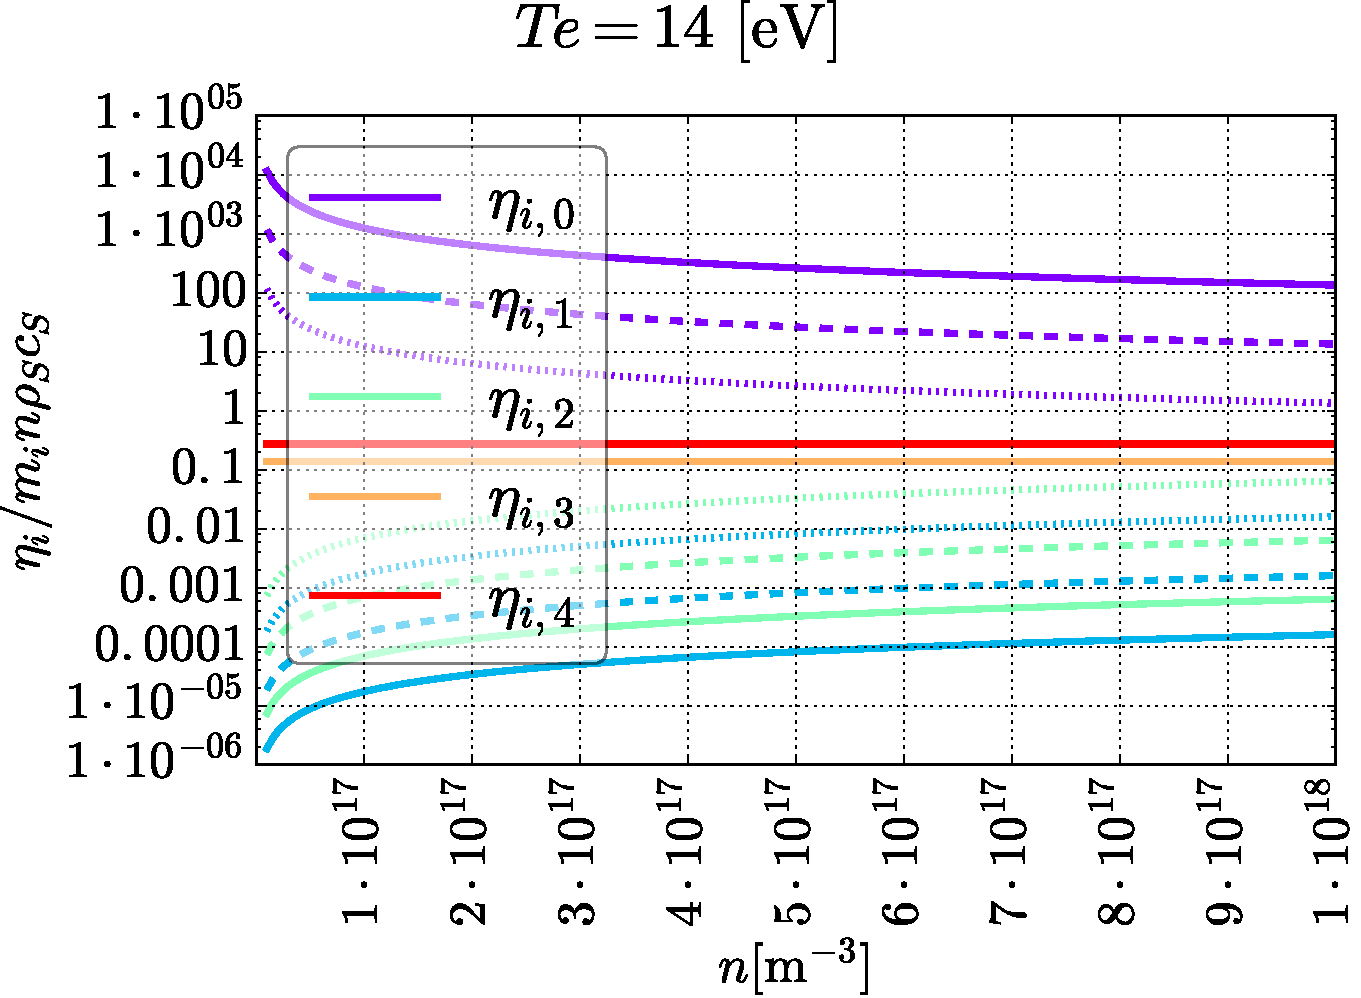
\includegraphics[width=1.0\textwidth]{fig/etaINScan}
        \caption{The normalized ion viscosities as a function of $n$}
    \end{subfigure}%
    \hfill
    \begin{subfigure}[t]{0.45\textwidth}
        \centering
        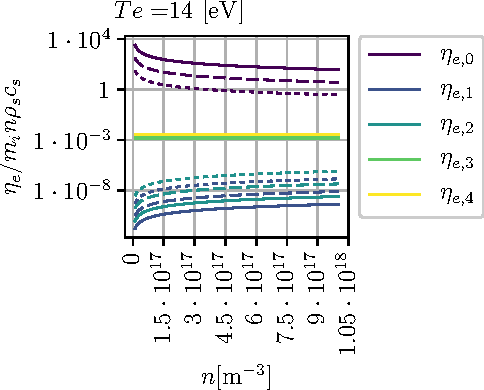
\includegraphics[width=1.0\textwidth]{fig/etaENScan}
        \caption{The normalized ion viscosities as a function of $n$}
    \end{subfigure}
    \\
    \hfill
    \begin{subfigure}[t]{0.45\textwidth}
        \centering
        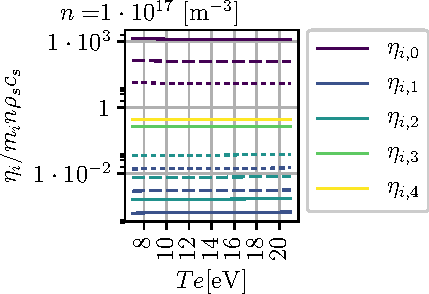
\includegraphics[width=1.0\textwidth]{fig/etaITScan}
        \caption{The normalized ion viscosities as a function of $T_e$}
    \end{subfigure}
    \hfill
    \begin{subfigure}[t]{0.45\textwidth}
        \centering
        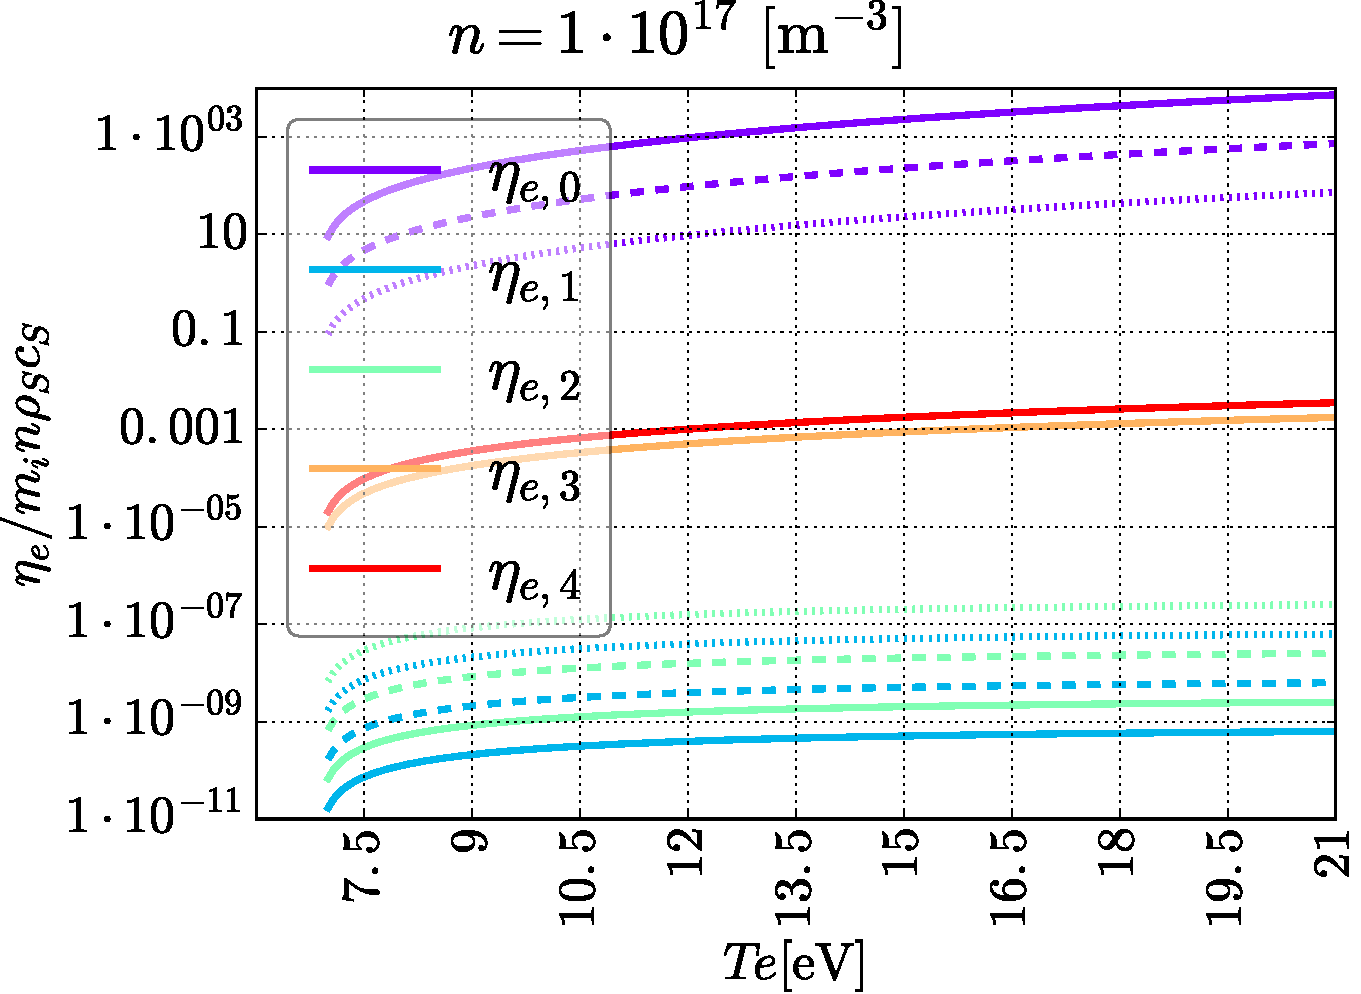
\includegraphics[width=1.0\textwidth]{fig/etaETScan}
        \caption{The normalized ion viscosities as a function of $T_e$}
    \end{subfigure}
    \caption{$\eta$ scans. The solid lines are taken at $B=1\text{ T}$, the
        dashed at $B=0.1\text{ T}$, and the dotted at $B=0.01\text{ T}$}
    \label{fig:etas}
\end{figure}
%
\begin{align*}
    \div\te{\pi}_\a
    \simeq&
    \quad
    \ve{e}_x
    \L(
       -\frac{\eta_{\a,0}}{3}
                       \L[\partial_x^2 u^{x}_{\a}
              + \partial_x\partial_y u^{y}_{\a}
              - 2\partial_x\partial_z u^{z}_{\a} \R]
    \R)
    %
    \\&+
    \ve{e}_y
    \L(
     -\frac{\eta_{\a,0}}{3}
                       \L[\partial_y\partial_x u^{x}_{\a}
              + \partial_y^2 u^{y}_{\a}
              - 2\partial_y\partial_z u^{z}_{\a} \R]
    \R)
    %
    \\&+
    \ve{e}_z
    \L(
    -\frac{2\eta_{\a,0}}{3}
        \L[
        2\partial_z^2 u^{z}_{\a} -
        \L(\partial_z\partial_x u^{x}_{\a}
           +\partial_z\partial_y u^{y}_{\a}
        \R)
        \R]
    \R)
\end{align*}
%
Using that to first order, only the $\ve{E}\times\ve{B}$ drift advects particles perpendiculary.
In Clebsch coordinates, we have that $\ve{u}_{E}$ is given by \cref{app:ExB}, which means that we get
%
\begin{align*}
    \ve{u}_E
    =&\frac{1}{JB}
           \L(
           - g_{zz}\ve{e}_y \partial_x
           + g_{zz}\ve{e}_x  \partial_y
           \R)
           \phi
   =\frac{1}{B}
           \L(
           - \ve{e}_y \partial_x
           + \ve{e}_x  \partial_y
           \R)
           \phi
    \\
    %
    u_{E}^{x} =& \frac{1}{B} \partial_y \phi
    \qquad
    u_{E}^{y} = -\frac{1}{B} \partial_x \phi
    \qquad
    u_{E}^{z} = 0
\end{align*}
%
We note that we are again operting with a left handed coordinate system.
Using this, we find that
%
\begin{align*}
    \div\te{\pi}_\a
    \simeq&
    \quad
    \ve{e}_x
    \L(
       -\frac{\eta_{\a,0}}{3}
                       \L[\frac{1}{B} \partial_x^2 \partial_y \phi
              - \frac{1}{B} \partial_x^2\partial_y \phi
              - 2\partial_x\partial_z u^{z}_{\a} \R]
    \R)
    %
    \\&+
    \ve{e}_y
    \L(
     -\frac{\eta_{\a,0}}{3}
                       \L[\frac{1}{B} \partial_y^2\partial_x \phi
              - \frac{1}{B} \partial_y^2 \partial_x \phi
              - 2\partial_y\partial_z u^{z}_{\a} \R]
    \R)
    %
    \\&+
    \ve{e}_z
    \L(
    -\frac{2\eta_{\a,0}}{3}
        \L[
        2\partial_z^2 u^{z}_{\a} -
        \frac{1}{B} \L(\partial_z\partial_x \partial_y \phi
           -\partial_z\partial_y \partial_x \phi
        \R)
        \R]
    \R)
    \\
    %
    %
    =&
    \quad
    \ve{e}_x \frac{2\eta_{\a,0}}{3} \partial_x\partial_z u^{z}_{\a}
    +
    \ve{e}_y \frac{2\eta_{\a,0}}{3} \partial_y\partial_z u^{z}_{\a}
    -
    \ve{e}_z
    \frac{4\eta_{\a,0}}{3} \partial_z^2 u^{z}_{\a}
    \numberthis
    \label{eq:piTensor}
\end{align*}
%
% FIXME: Check that this is actually the order
From our drift approximation, we found that the viscosity drift was of $\mathcal{O}(\e)$, and we therefore neglected it.
We will however use the parallel part of $\div\te{\pi}_\a$ (that is $\frac{4\eta_{\a,0}}{3} \partial_z^2 u^{z}_{\a}$) in the parallel momentum equations in order to have some diffusion in the system for numerical stability.


\chapter{The electrostatic approximation}
\label{app:elstat}
Rearranging \cref{fluideq:mom}, and multiplying it with $\frac{q_\a}{m_\a}$ yields
%
\begin{align*}
    q_{\a} \partial_t (n_{\a} \ve{u}_{\a})
    =&
    - q_{\a} \ve{u}_{\a} \partial_t n_{\a}
    - \frac{q_\a}{m_\a}\ve{u}_{\a}\cdot\nabla\ve{u}_{\a}
    - \frac{q_\a}{m_\a}\div \te{\pi}_{\a}
    - \frac{q_\a}{m_\a}\grad p_{\a}
    + \frac{q_\a^2}{m_\a} n_\a\L(\ve{E}  + \ve{u_\a}\times\ve{B}\R)
    \\ &
    + \frac{q_\a}{m_\a}\ve{R}_{\b\to \a}
    + \frac{q_\a}{m_\a}\ve{R}_{n\to \a}
    - q_\a S_{\a,n}\ve{u}_{\a}
\end{align*}
%
Adding the equation for electrons and ions using quasi-neutrality yields
%
\begin{align*}
    \partial_t \ve{J}
    =&
     \frac{\ve{J}}{n} \partial_t n
     \\&
    + \frac{e}{m_e}\ve{u}_{e}\cdot\nabla\ve{u}_{e}
    - \frac{e}{m_i}\ve{u}_{i}\cdot\nabla\ve{u}_{i}
     \\&
    + \frac{e}{m_e}\div \te{\pi}_{e}
    - \frac{e}{m_i}\div \te{\pi}_{i}
     \\&
    + \frac{e}{m_e}\grad p_{e}
    - \frac{e}{m_i}\grad p_{i}
     \\&
     + \frac{e^2}{m_e} n\L(-\grad{\phi}-\partial_t \ve{A}+ \ve{u_e}\times\ve{B}\R)
     + \frac{e^2}{m_i} n\L(-\grad{\phi}-\partial_t \ve{A}+ \ve{u_i}\times\ve{B}\R)
    \\ &
    - \frac{e}{m_e}\ve{R}_{i\to e}
    + \frac{e}{m_i}\ve{R}_{e\to i}
     \\&
    - \frac{e}{m_e}\ve{R}_{n\to e}
    + \frac{e}{m_i}\ve{R}_{n\to i}
     \\&
     + S \frac{\ve{J}}{n}
     \numberthis
     \label{eq:current_eq}
\end{align*}
%
where $\curl\ve{A}=\ve{B}$.
We then have that
%
\begin{align*}
    \curl\curl\ve{A}=&\curl\ve{B}
    \note{Low frequency}
    \\
    \grad^2\ve{A} - \grad(\div \ve{A})=&\mu_0\ve{J}
    \note{Coloumb gauge}
    % NOTE: See Griffiths
    \\
    \frac{\grad^2\ve{A}}{\mu_0}=&\ve{J}
    \\
    \ve{J} =& \frac{\div(\grad_\perp\ve{A}+\grad_\|\ve{A})}{\mu_0}
    \note{Assume $k_\perp \ll k_\|$}
    \\
    \ve{J} \simeq& \frac{\grad^2_\perp\ve{A}}{\mu_0}
    \numberthis
    \label{eq:coloumbGauge}
\end{align*}
%
Thus the LHS can be written
%
\begin{align*}
    \partial_t \ve{J} \simeq \partial_t \frac{\grad^2_\perp\ve{A}}{\mu_0}
\end{align*}
%
We can now use order of magnitude arguments to compare the size of the terms $\partial_t \frac{\grad^2_\perp\ve{A}}{\mu_0}$ and $\frac{e^2}{m_e}\partial_t \ve{A}$.
If the latter is larger than the former, it will mean that the time change of the magnetic field $\ve{B}$ will be a major contributor to the time change of the current $\ve{J}$, and electromagnetic effects be important%
%
\footnote{
    If the $\partial_t \ve{J}$ term was dominating (preferably by orders of magnitude), then there would be terms (or sum of terms) in \cref{eq:current_eq} which would be dominating the electromagnetic terms.
    Conversely, if the electromagnetic term was dominating, then the electromagnetic term would be dominating the sum of the other terms (not necessarily larger than each individual term, as terms may approximately cancel).
}.%
%
That is if
%
\begin{align*}
    \partial_t \frac{\grad^2_\perp\ve{A}}{\mu_0}
    < &
    \frac{ne^2}{m_e}\partial_t \ve{A}
    \\
    \rightarrow &
    \\
    \frac{1}{\omega_{ci}} \frac{k_\perp^2\ve{A}}{\mu_0}
    < &
    \frac{ne^2}{m_e}\frac{1}{\omega_{ci}} \ve{A}
    \\
    \frac{k_\perp^2}{\mu_0}
    < &
    \frac{ne^2}{m_e}
    \\
    k_\perp^2
    < &
    \frac{\mu_0ne^2}{m_e}
    \\
    k_\perp^2
    < &
    \frac{2m_i}{2m_i}\frac{B^2}{T_e}\frac{T_e}{B^2}\frac{\mu_0ne^2}{m_e}
    \\
    k_\perp^2
    < &
    \frac{m_i}{2m_e}\frac{e^2B^2}{m_iT_e}\frac{2\mu_0nT_e}{B^2}
    \\
    k_\perp^2
    < &
    \frac{m_i}{2m_e}\frac{1}{\rho_s^2}\b
\end{align*}
%
where the plasma beta ($\b$) is the kinetic pressure over the magnetic pressure.
As $ k_\perp^2\rho_s^2$ is typically in the order of unity for drift wave turbulence, we find that electromagnetic effects becomes important whenever
%
\begin{align*}
    1
    < &
    \frac{m_i}{2m_e}\b
    \\
    \frac{2m_e}{m_i}
    < &
    \b
\end{align*}
%
We observe that we get the identical condition if we choose to compare with $\frac{\ve{J}}{n}\partial_t n$ instead.
%FIXME; Consider to compare with other terms as well


\chapter{Parallel current equation with electromagnetic effects}
\label{app:elMag}
We will here continue the derivation of \cref{eq:curNormE} when keeping the $\partial_t A_\|$ term.
If we assume that $\grad_\perp^2 A_\| \gg \grad_\|^2 A_\|$, we have from \cref{eq:coloumbGauge} that
%
\begin{align*}
    \ve{b}\cdot\ve{J} \simeq& \ve{b}\cdot\frac{\grad^2_\perp\ve{A}}{\mu_0}
    \note{$\partial_i \ve{b} \simeq 0$}
    \\
    %
    j_\| \simeq& \frac{\grad^2_\perp A_\|}{\mu_0}
\end{align*}
%
We can normalize Amp{\`e}re's law, using $\ve{A}=\ve{\tilde{A}}\frac{T_e}{ec_s}$, which gives
%
\begin{align*}
   en_0c_s j_\|
   =&\frac{1}{\mu_0}\frac{1}{\rho_s^2} \frac{T_e}{ec_s} \grad^2_\perp A_\|\\
   =&\frac{1}{\mu_0}\frac{\om_{ci}^2}{c_s^2} \frac{T_e}{ec_s} \grad^2_\perp A_\|\\
    j_\|
   =&\frac{1}{\mu_0}\frac{\om_{ci}^2}{c_s^4} \frac{T_e}{e^2n_0} \grad^2_\perp A_\|\\
   =&\frac{1}{\mu_0}
     \frac{e^2B^2}{m_i^2}
      \frac{m_i^2}{T_e^2}
      \frac{T_e}{e^2n_0}
      \grad^2_\perp A_\|\\
   =& \frac{B^2}{\mu_0}
      \frac{1}{T_e}
      \frac{1}{n_0}
      \grad^2_\perp A_\|\\
   =&\frac{2}{2}
     \frac{B^2}{\mu_0T_en_0}
      \grad^2_\perp A_\|\\
   =&\frac{2}{\b}
      \grad^2_\perp A_\|
\end{align*}
%
This equation can now be inverted in order to obtain $A_\|$.
In other words, \cref{eq:curNormE} can be rewritten to
%
\begin{align*}
 \partial_t j_\|
=&
 - \frac{1}{JB}\L\{\phi, j_{\|}\R\}
 -   u_{i,\|}\partial_\|\L( n \L[u_{i,\|}+ u_{e,\|} \R]\R)
 + 2 u_{e,\|}\partial_\|\L( n  u_{e,\|} \R)
   \\&
 - 0.51 \nu_{ei}j_\|
   + \mu T_e \partial_\| n
   + \mu n \L(-\partial_\|\phi-\partial_tA_\|\R)
 + n \L(\nu_{e n}u_{e,\|} - \nu_{i n}u_{i,\|} \R)
 \\
=&
 - \frac{1}{JB}\L\{\phi, j_{\|}\R\}
 -   u_{i,\|}\partial_\|\L( n \L[u_{i,\|}+ u_{e,\|} \R]\R)
 + 2 u_{e,\|}\partial_\|\L( n  u_{e,\|} \R)
   \\&
 - 0.51 \nu_{ei}j_\|
   + \mu T_e \partial_\| n
   - \mu n \partial_\|\phi - \partial_t \mu \L( n A_\| \R) + \mu A_\| \partial_t n
 + n \L(\nu_{e n}u_{e,\|} - \nu_{i n}u_{i,\|} \R)
 \\
 \partial_t \L(j_\|+ \mu n A_\| \R)
=&
 - \frac{1}{JB}\L\{\phi, j_{\|}\R\}
 -   u_{i,\|}\partial_\|\L( n \L[u_{i,\|}+ u_{e,\|} \R]\R)
 + 2 u_{e,\|}\partial_\|\L( n  u_{e,\|} \R)
   \\&
 - 0.51 \nu_{ei}j_\|
   + \mu \L(T_e \frac{n}{n}\partial_\| n
   - n \partial_\|\phi + A_\| \frac{n}{n} \partial_t [n] \R)
 + n \L(\nu_{e n}u_{e,\|} - \nu_{i n}u_{i,\|} \R)
 \note{$T_e$ constant}
 \\
 \partial_t j^M_\|
=&
 - \frac{1}{JB}\L\{\phi, j_{\|}\R\}
 -   u_{i,\|}\partial_\|\L( n \L[u_{i,\|}+ u_{e,\|} \R]\R)
 + 2 u_{e,\|}\partial_\|\L( n  u_{e,\|} \R)
   \\&
 - 0.51 \nu_{ei}j_\|
   + \mu n \L(\partial_\|\L[ T_e\ln(n) - \phi\R]
   + A_\| \partial_t \ln[n] \R)
   + n \L(\nu_{e n}u_{e,\|} - \nu_{i n}u_{i,\|} \R)
\end{align*}
%
where $j^M_\| = j_\|+ \mu n A_\|$.
%
For numerical purposes, in order for $A_\|$ not to be much bigger than the rest of the quantities, it is common practice to renormalize $A_{\|, \text{old}} = \frac{1}{2}\b A_{\|, \text{new}}$.
Dropping the $_{\text{new}}$ subscript yields %
%
\begin{align*}
    j_\| =& \grad^2_\perp A_\|\\
    j^M_\| =& j_\|+ \frac{1}{2}\b\mu n A_\|
\end{align*}


\chapter{Energies}
\label{app:energies}
We will in this appendix briefly comment on the energy of the system.
One should note that the CELMA equations are probably not energy conserving, and we have argued that this may be of lesser importance as the system is driven by its sources and its sinks.
An energy conserving system has the nice property that one could identify which parts of the equation transfers energy.
This can be done by multiplying the time evolving fields with various variables such that the resulting evolution would have the units of energy density.
One could then integrate over the volume and see which terms transfers energy to each other.
Another approach is to simply derive the set of equation from energy principles by using the variational principle of the Lagrangian of the system.

In this thesis, however, we will only be using the kinetic and potential energy arising from the pressure.
Thus saying something about the energy arising from the source etc. is outside the scope of this thesis.

\section{The kinteic energy}
%
We will now define the energy density $\mathcal{E}_{\text{kin},\a}$.
From this, we will see what part of the energy density which arises due to fluctuations, and which part which arise from the mean.
We can then integrate the energy densities over the volume to get the expressions for the energy.

\subsection{The kinteic energy density}
The energy density is defined as
%
\begin{align*}
    \mathcal{E}_{\text{kin},\a} &= \frac{1}{2}m_an \ve{u}^2_\a.
\end{align*}
%
If we now let $\expt{A}$ denote the poloidal average of $A$, defined in \cref{sec:polAvg}, and use the notation
%
\begin{align*}
    \wt{A} = A - \expt{A},
\end{align*}
%
so that $A = \expt{A} + \wt{A}$.
We get that
%
\begin{align*}
     \mathcal{E}_{\text{kin},\a} =& \frac{1}{2}m_\a n\ve{u}_\a^2\\
     %
     =& \frac{1}{2}m_\a\L(\expt{n} + \wt{n}\R)
            \L(\expt{\ve{u}}_\a + \wt{\ve{u}}_\a\R)^2\\
     %
     =& \frac{1}{2}m_\a\L(\expt{n} + \wt{n}\R)
            \L(\expt{\ve{u}_\a}^2
             + 2\wt{\ve{u}}_\a\cdot\expt{\ve{u}_\a}
             + \wt{\ve{u}}_\a^2
            \R)\\
     %
     =& \frac{1}{2}m_\a\L(\expt{n} \expt{\ve{u}_\a}^2
             + 2 \expt{n} \wt{\ve{u}}_\a\cdot\expt{\ve{u}_\a}
             + \expt{n}\wt{\ve{u}}_\a^2
             +
             \wt{n} \expt{\ve{u}_\a}^2
             + 2 \wt{n} \wt{\ve{u}}_\a\cdot\expt{\ve{u}_\a}
             + \wt{n}\wt{\ve{u}}_\a^2\R).
        \numberthis
        \label{eq:enDensExpanded}
\end{align*}
%
We can now split this into an average and a fluctuation around the mean.
We demand that this satisfies
%
\begin{align}
    \mathcal{E}_{\text{kin},\a} &= \expt{\mathcal{E}_{\text{kin},\a}} + \wt{\mathcal{E}}_{\text{kin},\a}
    \label{eq:eDensDefinition}
    \\
    \expt{\expt{\mathcal{E}_{\text{kin},\a}}} &= \expt{\mathcal{E}_{\text{kin},\a}}
    \label{eq:avgOfAvg}
    \\
    \expt{\wt{\mathcal{E}}_{\text{kin},\a}} &= 0.
    \label{eq:zeroFluct}
\end{align}
%
By noting that $\expt{a}$ in general is a constant with respect to the integration limit, we have that
%
\begin{align*}
    \expt{\expt{a}\wt{b}} = \expt{a}\expt{\wt{b}} = \expt{a}\cdot0 = 0.
\end{align*}
%
This means that the terms in \cref{eq:enDensExpanded} with only one fluctuating factor belongs to $\wt{\mathcal{E}}_{\text{kin},\a}$ as it satisfies \cref{eq:zeroFluct}.
However, we have that $\expt{\wt{a}\wt{b}}$ (the covariance of $a$ and $b$) in general is not equal to $0$.
For example in the case where $a=b$, the product $\wt{a}\wt{a}$ can never be negative, so that $\expt{\wt{a}\wt{a}} = 0 \iff \wt{a}=0$.
Hence, these terms contributes partly to the average and partly to the fluctuations.

We can now write \cref{eq:enDensExpanded} as
%
\begin{align*}
     \mathcal{E}_{\text{kin},\a} =
        \frac{1}{2}m_\a\L(\R.&
            \expt{n} \expt{\ve{u}_\a}^2
             + 2 \wt{\ve{u}}_\a\cdot \expt{n} \expt{\ve{u}_\a}
             + \wt{n} \expt{\ve{u}_\a}^2
             \\
             &
             + \expt{n}\wt{\ve{u}}_\a^2
             + \expt{\expt{n}\wt{\ve{u}}_\a^2}
             - \expt{\expt{n}\wt{\ve{u}}_\a^2}
             \\
             &
             + 2 \wt{n} \wt{\ve{u}}_\a\cdot\expt{\ve{u}_\a}
             + \expt{2 \wt{n} \wt{\ve{u}}_\a\cdot\expt{\ve{u}_\a}}
             - \expt{2 \wt{n} \wt{\ve{u}}_\a\cdot\expt{\ve{u}_\a}}
             \\
             &\L.
             + \wt{n}\wt{\ve{u}}_\a^2
             + \expt{\wt{n}\wt{\ve{u}}_\a^2}
             - \expt{\wt{n}\wt{\ve{u}}_\a^2}
             \R).
\end{align*}
%
Rewriting yields
%
\begin{align*}
     &\mathcal{E}_{\text{kin},\a} =
     \\&
        \frac{1}{2}m_\a\L(
            \expt{n} \expt{\ve{u}_\a}^2
             + \expt{\expt{n}\wt{\ve{u}}_\a^2}
             + \expt{2 \wt{n} \wt{\ve{u}}_\a\cdot\expt{\ve{u}_\a}}
             + \expt{\wt{n}\wt{\ve{u}}_\a^2}
        \R)
             \\
             &+
        \frac{1}{2}m_\a\L(
              2 \wt{\ve{u}}_\a\cdot \expt{n} \expt{\ve{u}_\a}
             + \wt{n} \expt{\ve{u}_\a}^2
             +
             \L[\expt{n}\wt{\ve{u}}_\a^2
                - \expt{\expt{n}\wt{\ve{u}}_\a^2}
             \R]
             +
             \L[2 \wt{n} \wt{\ve{u}}_\a\cdot\expt{\ve{u}_\a}
                - \expt{2 \wt{n} \wt{\ve{u}}_\a\cdot\expt{\ve{u}_\a}}
             \R]
             +
             \L[
               \wt{n}\wt{\ve{u}}_\a^2
             - \expt{\wt{n}\wt{\ve{u}}_\a^2}
             \R]
             \R).
\end{align*}
%
We can now identify the first term as
%
\begin{align}
     \expt{\mathcal{E}_{\text{kin},\a}} =
        \frac{1}{2}m_\a\L(
            \expt{n} \expt{\ve{u}_\a}^2
             + \expt{\expt{n}\wt{\ve{u}}_\a^2}
             + \expt{2 \wt{n} \wt{\ve{u}}_\a\cdot\expt{\ve{u}_\a}}
             + \expt{\wt{n}\wt{\ve{u}}_\a^2}
        \R)
    \label{eq:enDensAvg}
\end{align}
%
and the second term as
%
\begin{align*}
    \wt{\mathcal{E}}_{\text{kin},\a} =
    \frac{1}{2}m_\a\L( \R.  &
              2 \wt{\ve{u}}_\a\cdot \expt{n} \expt{\ve{u}_\a}
             + \wt{n} \expt{\ve{u}_\a}^2
             +
             \\
             &
             \L.
             \L[\expt{n}\wt{\ve{u}}_\a^2
                - \expt{\expt{n}\wt{\ve{u}}_\a^2}
             \R]
             +
             \L[2 \wt{n} \wt{\ve{u}}_\a\cdot\expt{\ve{u}_\a}
                - \expt{2 \wt{n} \wt{\ve{u}}_\a\cdot\expt{\ve{u}_\a}}
             \R]
             +
             \L[
               \wt{n}\wt{\ve{u}}_\a^2
             - \expt{\wt{n}\wt{\ve{u}}_\a^2}
             \R]
             \R).
     \numberthis
    \label{eq:enDensFluct}
\end{align*}
%
We observe that \cref{eq:enDensAvg} and \cref{eq:enDensFluct} satisfies \cref{eq:zeroFluct,eq:avgOfAvg,eq:eDensDefinition}.

Next, we have that the energy is given as the energy density integrated over the volume.
Thus
%
\begin{align*}
    E_{\text{kin},\a}
    = \inde{\mathcal{E}_{\text{kin},\a}}{V}
    = \inde{\expt{\mathcal{E}_{\text{kin},\a}}}{V} + \inde{\wt{\mathcal{E}}_{\text{kin},\a}}{V}
    = \expt{E_{\text{kin},\a}} + \wt{E}_{\text{kin},\a},
\end{align*}
%
where
%
\begin{align*}
    \expt{E_{\text{kin},\a}} =& \inde{\expt{\mathcal{E}_{\text{kin},\a}}}{V}\\
    \wt{E}_{\text{kin},\a} =& \inde{\wt{\mathcal{E}}_{\text{kin},\a}}{V}.
\end{align*}
%
In cylindrical coordinates, we have that
%
\begin{align*}
    \inde{f}{V} = \iiint f J \d\rho \d\theta \d z,
\end{align*}
%
that
%
\begin{align*}
    \inde{\expt{f}}{V}
    =& \iiint \expt{f} J \d\rho \d\theta \d z\\
    =& \iiint \frac{\defi{0}{2\pi}{f}{\theta}}{2\pi} J \d\theta \d\rho \d z\\
    =& \int_0^{L_z} \int_0^{L_\rho} \int_0^{2\pi} \frac{\defi{0}{2\pi}{f}{\theta}}{2\pi} J \d\theta \d\rho \d z\\
    =& \int_0^{L_z} \int_0^{L_\rho} \frac{\defi{0}{2\pi}{f}{\theta}}{2\pi} J\int_0^{2\pi}  \d\theta \d\rho \d z\\
    =& \int_0^{L_z} \int_0^{L_\rho} \frac{\defi{0}{2\pi}{f}{\theta}}{2\pi}2\pi J \d\rho \d z\\
    =& \int_0^{L_z} \int_0^{L_\rho} \defi{0}{2\pi}{f}{\theta} J \d\rho \d z\\
    =& \inde{f}{V},
    \numberthis
    \label{eq:intExptF}
\end{align*}
%
and that
%
\begin{align*}
    \inde{\wt{f}}{V}
    =& \iiint \wt{f} J \d\rho \d\theta \d z\\
    =& \int_0^{L_z} \int_0^{L_\rho} \int_0^{2\pi}\wt{f} \d\theta J \d\rho \d z\\
    =& \int_0^{L_z} \int_0^{L_\rho} \frac{\int_0^{2\pi} \wt{f} \d\theta}{2\pi}2\pi J \d\rho \d z\\
    =& \int_0^{L_z} \int_0^{L_\rho} \expt{\wt{f}} 2\pi  J \d\rho \d z\\
    =& 0.
    \numberthis
    \label{eq:intAvgF}
\end{align*}
%
In other words, we have that
%
\begin{align*}
    \wt{E}_{\text{kin},\a} =& 0\\
    \expt{E_{\text{kin},\a}} =& E_{\text{kin},\a}.
\end{align*}

\subsection{The global kinteic energy}
%
Due to gyroviscous cancellation, we have that, to first order, only the $E\times B$-drift carries particles.
This gives
%
\begin{align*}
    E_{\text{kin},\a}
    =& \frac{1}{2}m_{\a}\int
       n\mathbf{u}_E^2
       + n\mathbf{u}_{\a,\parallel}^2 \d V
     \\
    =& \frac{1}{2}m_{\a}\int
       n\left(\frac{-\nabla_\perp\phi
              \times\mathbf{b}}{B}\right)^2
       + n\mathbf{u}_{\a,\parallel}^2 \d V
    \\
    =& \frac{1}{2}m_{\a}\int
       n\left(\left[\frac{-\nabla_\perp\phi}{B}\right]^2
       + [\mathbf{u}_{\a,\parallel}]^2\right) \d V
   \\
    =& \frac{1}{2}m_{\a}\iiint
       n\left(\left[\frac{-\nabla_\perp\phi}{B}\right]^2
       + [\mathbf{u}_{\a,\parallel}]^2\right)
       J \d\rho \d\theta \d z
    \\
    =& \frac{1}{2}m_i\frac{m_{\a}}{m_i}
       n_0c_s^2\rho_s^3
       \iiint
       \breve{n}\breve{u}_\a^2
       \breve{J} \d \breve{\rho} \d\theta \d \breve{z}
    \\
    =& m_in_0c_s^2\rho_s^3 \breve{E}_{\text{kin},\a}
    \\
    =& n_0T_{e,0}\rho_s^3 \breve{E}_{\text{kin},\a},
\end{align*}
%
where we have used (V.4) in \cite{Dhaeseleer1991book}, $\a$ denotes the particle species, and where $\breve{E}_{\text{kin},\a} = \frac{m_{\a}}{m_i}\iiint \breve{n}\breve{u}_\a^2 \breve{J} \d \breve{\rho} \d\theta \d \breve{z}$.

%
\section{The potential energy}
%
The potential energy is given by the kinetic pressure $nT$
%
\footnote{In \cite{Wiesenberger2014} it is stated that the potential energy can be obtained from the Helmholtz free equation, and reads $E_{\text{pot}}=nT_e\log(n)$.
    However, this depends on the partition function used, and one can show that for a more "standard" partition function $E_{\text{pot}}=nT_e\log(n)$ as shown in \cite{Kittel1980book}.}%
.
As $T_i=0$, only the electrons will give rise to the potential energy.

\subsection{The potential energy density}
The potential energy density from the pressure is given by%
%
\begin{align*}
    \mathcal{E}_{\text{pot}} =& nT_e.
\end{align*}
%
Since we use a constant $T_e$, we get that $T_e=\expt{T_e}$.
Hence
%
\begin{align*}
    &\wt{\mathcal{E}}_{\text{pot}} = \wt{n}T_e&
    &\expt{\mathcal{E}_{\text{pot}}} = \expt{n}T_e&
\end{align*}
%
and
%
\begin{align*}
    E_{\text{pot}}
    = \inde{\mathcal{E}_{\text{pot}}}{V}
    = \inde{\expt{\mathcal{E}_{\text{pot}}}}{V} + \inde{\wt{\mathcal{E}}_{\text{pot}}}{V}
    = \expt{E_{\text{pot}}} + \wt{E}_{\text{pot}},
\end{align*}
%
where
%
\begin{align*}
    \expt{E_{\text{pot}}} =& \inde{\expt{\mathcal{E}_{\text{pot}}}}{V}\\
    \wt{E}_{\text{pot}} =& \inde{\wt{\mathcal{E}}_{\text{pot}}}{V}.
\end{align*}
%
Due to \cref{eq:intExptF,eq:intAvgF}, we have that
%
\begin{align*}
    \wt{E}_{\text{pot}} =& 0\\
    \expt{E_{\text{pot}}} =& E_{\text{pot}}.
\end{align*}

\subsection{The global potential energy}
%
The global potential energy is therefore given by
%
\begin{align*}
    E_{\text{pot}}
    =& \int nT_e \d V
    \\
    =& \iiint nT_e J \d\rho \d\theta \d z
    \\
    =& n_0T_{e,0}\rho_s^3\iiint \breve{n}\breve{T}_e \breve{J} \d\breve{\rho} \d\theta \d \breve{z}
    \\
    =& n_0T_{e,0}\rho_s^3\breve{E}_{\text{pot}}.
\end{align*}


\chapter{The coordinate system}
\label{app:coord}
The coordinates in a cylindrical geometry are written\\
%
\begin{minipage}{0.4\textwidth}
\begin{align*}
    x=&\rho \cos\theta\\
    y=&\rho \sin\theta\\
    z=& z
\end{align*}
\end{minipage}
\hfill
\begin{minipage}{0.4\textwidth}
\begin{align*}
    \rho=& \sqrt{x^2+y^2}\\
    \theta=&\atan\L(\frac{y}{x}\R)\\
    z=& z
\end{align*}
\end{minipage}

\section{The metrics}
\label{sec:metr}
%
We have that
%
\begin{align*}
    &\ve{e}_i = \partial_i&
    &\ve{e}^i = \d u_i&
\end{align*}
%
where $u_i$ is the set of the coordinate curves

To coordinate transform a covariant basis vector, we can consider an arbitrary line $f$ passing through the point under consideration written in the new set of coordinates.
We then use the chain rule to determine how the basis vector is written in the new set of coordinates.
We have
%
\begin{align*}
    \parti{f(\rho, \theta, z)}{x_i}
    =
    \parti{f}{\rho} \parti{\rho}{x_i}
    + \parti{f}{\theta} \parti{\theta}{x_i}
    + \parti{f}{z} \parti{z}{x_i}
\end{align*}
%
as the line $f$ is arbitrary, we have
%
\begin{align*}
    \ve{e}_i
    =
    \parti{}{x_i}
    =
    %
    \parti{\rho}{x_i} \parti{}{\rho}
    + \parti{\theta}{x_i} \parti{}{\theta}
    + \parti{z}{x_i} \parti{}{z}
    %
    =
    %
    \parti{\rho}{x_i} \ve{e}_{\rho}
    + \parti{\theta}{x_i} \ve{e}_{\theta}
    + \parti{z}{x_i} \ve{e}_{z}
    %
\end{align*}
%
where in our case $x_i \in \{x,y,z\}$.

To coordinate transform a contravariant basis vector, we can apply the chain rule directly to determine how the basis vector is written in the new set of coordinates.
We have
%
\begin{align*}
    \ve{e}^i
    =
    \d u^i(x,y,z)
    =
    %
    \parti{u_i}{x}\d x
    + \parti{u_i}{y}\d y
    + \parti{u_i}{z}\d z
    %
    =
    %
    \parti{u_i}{x}\ve{e}^x
    + \parti{u_i}{y}\ve{e}^y
    + \parti{u_i}{z}\ve{e}^z
    %
\end{align*}
%
At this point we note that there are no difference between co and contravariant basis vectors in a Cartesian coordinate system.

In the following, we are going to make use of the following relations
\\
%
\begin{minipage}{0.4\textwidth}
\begin{align*}
    \partial_x \rho
    =&
    \partial_x \sqrt{x^2+y^2}
    =
    \frac{x}{\rho}
    =
    \cos\theta\\
    %
    \partial_y \rho
    =&
    \partial_y \sqrt{x^2+y^2}
    =
    \frac{y}{\rho}
    =
    \sin\theta
    \\
    %
    \partial_z \rho
    =&
    \partial_z \sqrt{x^2+y^2}
    =
    0
    \\
    %
    %
    \partial_x \theta
    =&
    \partial_x \atan\L(\frac{y}{x}\R)
    =
    -\frac{y}{\rho^2}
    =
    -\frac{1}{\rho}\sin\theta
    \\
    %
    \partial_y \theta
    =&
    \partial_y \atan\L(\frac{y}{x}\R)
    =
    \frac{x}{\rho^2}
    =
    \frac{1}{\rho}\cos\theta
    \\
    %
    \partial_z \theta
    =&
    \partial_z \atan\L(\frac{y}{x}\R)
    =
    0
    \\
\end{align*}
\end{minipage}
%
\hfill
%
\begin{minipage}{0.4\textwidth}
\begin{align*}
    \partial_\rho x
    =&
    \partial_\rho \rho\cos\theta
    =
    \cos\theta\\
    %
    \partial_\rho y
    =&
    \partial_\rho \rho\sin\theta
    =
    \sin\theta
    \\
    %
    \partial_\rho z
    =&
    0
    \\
    %
    %
    \partial_\theta x
    =&
    \partial_\theta \rho\cos\theta
    =
    -\rho\sin\theta
    \\
    %
    \partial_\theta y
    =&
    \partial_\theta \rho\sin\theta
    =
    \rho\cos\theta
    \\
    %
    \partial_\theta z
    =&
    0
\end{align*}
\end{minipage}\\
%
This means that a basis vector written in a Cartesian basis can be written with a covariant basis vector using cylindrical coordinates as
%
\begin{align*}
    \ve{e}_x
    &=
    \parti{\rho}{x} \ve{e}_{\rho}
    + \parti{\theta}{x} \ve{e}_{\theta}
    + \parti{z}{x} \ve{e}_{z}
    %
    =
    \cos\theta \ve{e}_\rho
    - \frac{1}{\rho} \sin\theta \ve{e}_\theta
    \\
%
%
    \ve{e}_y
    &=
    \parti{\rho}{y} \ve{e}_{\rho}
    + \parti{\theta}{y} \ve{e}_{\theta}
    + \parti{z}{y} \ve{e}_{z}
    %
    =
    \sin\theta \ve{e}_\rho
    + \frac{1}{\rho} \cos\theta \ve{e}_\theta
    \\
%
%
    \ve{e}_z
    &=
    \parti{\rho}{z} \ve{e}_{\rho}
    + \parti{\theta}{z} \ve{e}_{\theta}
    + \parti{z}{z} \ve{e}_{z}
    %
    =
    \ve{e}_z
\end{align*}
%
For the back transformation we have
%
\begin{align*}
    \ve{e}_\rho
    &=
    \parti{x}{\rho} \ve{e}_{x}
    + \parti{y}{\rho} \ve{e}_{y}
    + \parti{z}{\rho} \ve{e}_{z}
    %
    =
    \cos\theta \ve{e}_x
    + \sin\theta \ve{e}_y
    \\
%
%
    \ve{e}_\theta
    &=
    \parti{x}{\theta} \ve{e}_{x}
    + \parti{y}{\theta} \ve{e}_{y}
    + \parti{z}{\theta} \ve{e}_{z}
    %
    =
    -\rho\sin\theta \ve{e}_x
    + \rho\cos\theta \ve{e}_y
    \\
%
%
    \ve{e}_z
    &=
    \parti{x}{z} \ve{e}_{x}
    + \parti{y}{z} \ve{e}_{y}
    + \parti{z}{z} \ve{e}_{z}
    %
    =
    \ve{e}_z
\end{align*}
%
Further, a basis vector written in a Cartesian basis can be written with a contravariant basis vector using cylindrical coordinates as
%
\begin{align*}
    \ve{e}^\rho
    &=
    \parti{\rho}{x} \ve{e}^{x}
    + \parti{\rho}{y} \ve{e}^{y}
    + \parti{\rho}{z} \ve{e}^{z}
    %
    =
    \cos\theta \ve{e}^x
    + \sin\theta \ve{e}^y
    \\
%
%
    \ve{e}^\theta
    &=
    \parti{\theta}{x} \ve{e}^{x}
    + \parti{\theta}{y} \ve{e}^{y}
    + \parti{\theta}{z} \ve{e}^{z}
    %
    =
    -\frac{1}{\rho}\sin\theta \ve{e}^x
    + \frac{1}{\rho} \cos\theta \ve{e}^y
    \\
%
%
    \ve{e}^z
    &=
    \parti{z}{x} \ve{e}^{x}
    + \parti{z}{y} \ve{e}^{y}
    + \parti{z}{z} \ve{e}^{z}
    %
    =
    \ve{e}^z
\end{align*}
%
The covariant metric tensor $g^{ij}=\ve{e}^i\cdot\ve{e}^j$ and the contravariant metric tensor $g_{ij}=\ve{e}_i\cdot\ve{e}_j$ can now be computed.
For the contravariant components, we get
%
\begin{align*}
    g^{\rho\rho}
    =&
    \L(
      \cos\theta\ve{e}^x
      + \sin\theta\ve{e}^y
    \R)
    \cdot
    \L(
      \cos\theta\ve{e}^x
      + \sin\theta\ve{e}^y
    \R)
    =
      \cos^2\theta
      + \sin^2\theta
    =
    1
    \\
    %
    g^{\rho\theta}
    =&
    g^{\theta\rho}
    =
    \L(
      \cos\theta\ve{e}^x
      + \sin\theta\ve{e}^y
    \R)
    \cdot
    \L(
      -\frac{1}{\rho}\cos\theta\ve{e}^x
      + \frac{1}{\rho}\sin\theta\ve{e}^y
    \R)
    =
      -\frac{1}{\rho}\cos\theta\sin\theta
      + \frac{1}{\rho}\sin\theta\cos\theta
    =
    0
    \\
    %
    g^{\rho z}
    =&
    g^{z \rho}
    =
    \L(
      \cos\theta\ve{e}^x
      + \sin\theta\ve{e}^y
    \R) \cdot \ve{e}^z = 0
    \\
    %
    %
    %
    g^{\theta\theta}
    =&
    \L(
      -\frac{1}{\rho}\cos\theta\ve{e}^x
      + \frac{1}{\rho}\sin\theta\ve{e}^y
    \R)
    \cdot
    \L(
      -\frac{1}{\rho}\cos\theta\ve{e}^x
      + \frac{1}{\rho}\sin\theta\ve{e}^y
    \R)
    =
      \frac{1}{\rho^2}\cos^2\theta
      + \frac{1}{\rho^2}\sin^2\theta
    =
    \frac{1}{\rho^2}
    \\
    %
    g^{z\theta}
    =&
    g^{\theta z}
    =
    \L(
      -\frac{1}{\rho}\cos\theta\ve{e}^x
      + \frac{1}{\rho}\sin\theta\ve{e}^y
    \R) \cdot \ve{e}^z = 0
    \\
    %
    %
    %
    g^{z z}
    =&
    \ve{e}^z \cdot \ve{e}^z =1
\end{align*}
%
And for the covariant components, we get
%
\begin{align*}
    g_{\rho\rho}
    =&
    \L(
      \cos\theta\ve{e}_x
      + \sin\theta\ve{e}_y
    \R)
    \cdot
    \L(
      \cos\theta\ve{e}_x
      + \sin\theta\ve{e}_y
    \R)
    =
      \cos^2\theta
      + \sin^2\theta
    =
    1
    \\
    %
    g_{\rho\theta}
    =&
    g_{\theta\rho}
    =
    \L(
      \cos\theta\ve{e}_x
      + \sin\theta\ve{e}_y
    \R)
    \cdot
    \L(
      -\rho\sin\theta\ve{e}_x
      + \rho\cos\theta\ve{e}_y
    \R)
    =
      -\rho\cos\theta\sin\theta
      + \rho\sin\theta\cos\theta
    =
    0
    \\
    %
    g_{\rho z}
    =&
    g_{z \rho}
    =
    \L(
      \cos\theta\ve{e}_x
      + \sin\theta\ve{e}_y
    \R) \cdot \ve{e}_z = 0
    \\
    %
    %
    %
    g_{\theta\theta}
    =&
    \L(
      -\rho\sin\theta\ve{e}_x
      + \rho\cos\theta\ve{e}_y
    \R)
    \cdot
    \L(
      -\rho\sin\theta\ve{e}_x
      + \rho\cos\theta\ve{e}_y
    \R)
    =
      \rho^2\cos^2\theta
      + \rho^2\sin^2\theta
    =
    \rho^2
    \\
    %
    g_{z\theta}
    =&
    g_{\theta z}
    =
    \L( -\rho\sin\theta\ve{e}_x
      + \rho\cos\theta\ve{e}_y \R) \cdot \ve{e}_z
    =
    0
    \\
    %
    g_{z z} =&
    \ve{e}_z \cdot \ve{e}_z =1
\end{align*}
%
The Jacobian
%
\begin{align*}
    J=\sqrt{\det(g_{ij})}=\rho
\end{align*}
%
Finally, we calculate the derivatives of the contravariant basis vectors.
From what is calculated above, we see that $\partial_z e^i=0$ and $\partial_i e^z=0$.
The other basis vectors gives
%
\begin{align*}
    \partial_\rho \ve{e}^\theta
    &=&
    \partial_\rho
    \L( - \frac{1}{\rho} \sin\theta \ve{e}^x
        + \frac{1}{\rho} \cos\theta \ve{e}^y \R)
    =
        \frac{\sin\theta}{\rho^2} \ve{e}^x
        - \frac{\cos\theta}{\rho^2} \ve{e}^y
    =
    - \frac{1}{\rho}
    \L( - \frac{1}{\rho} \sin\theta \ve{e}^x
        + \frac{1}{\rho} \cos\theta \ve{e}^y \R)
    &=&
    - \frac{1}{\rho} \ve{e}^\theta
    \\
    %
    \partial_\rho \ve{e}^\rho
    &=&
    \partial_\rho
    \L( \cos\theta \ve{e}^x
        + \sin\theta \ve{e}^y \R)
    &=&
    0
    \\
    %
    \partial_\theta \ve{e}^\theta
    &=&
    \partial_\theta
    \L( - \frac{1}{\rho} \sin\theta \ve{e}^x
        + \frac{1}{\rho} \cos\theta \ve{e}^y \R)
    =
    \L( - \frac{1}{\rho} \cos\theta \ve{e}^x
        - \frac{1}{\rho} \sin\theta \ve{e}^y \R)
    =
    - \frac{1}{\rho}
    \L( \cos\theta \ve{e}^x
        + \sin\theta \ve{e}^y \R)
    &=&
    - \frac{1}{\rho}
    \ve{e}^\rho
    \\
    %
    \partial_\theta \ve{e}^\rho
    &=&
    \partial_\theta
    \L( \cos\theta \ve{e}^x
        + \sin\theta \ve{e}^y \R)
    =
        - \sin\theta \ve{e}^x
        + \cos\theta \ve{e}^y
    =
    \rho
    \L( - \frac{1}{\rho} \sin\theta \ve{e}^x
        + \frac{1}{\rho} \cos\theta \ve{e}^y \R)
    &=&
    \rho
    \ve{e}^\theta
\end{align*}
%

\subsection{Summary}
\label{app:cylSummary}
%
Basis vector transformations\\
%
\begin{minipage}{0.3\textwidth}
\begin{align*}
    \ve{e}_x
    &=
    \cos\theta \ve{e}_\rho
    - \frac{1}{\rho} \sin\theta \ve{e}_\theta
    \\
%
%
    \ve{e}_y
    &=
    \sin\theta \ve{e}_\rho
    + \frac{1}{\rho} \cos\theta \ve{e}_\theta
    \\
%
%
    \ve{e}_z &= \ve{e}_z
\end{align*}
\end{minipage}
%
\hfill
%
\begin{minipage}{0.3\textwidth}
    \begin{align*}
        \ve{e}_\rho
        &=
        \cos\theta \ve{e}_x
        + \sin\theta \ve{e}_y
        \\
    %
    %
        \ve{e}_\theta
        &=
        -\rho\sin\theta \ve{e}_x
        + \rho\cos\theta \ve{e}_y
        \\
    %
    %
        \ve{e}_z &= \ve{e}_z
    \end{align*}
\end{minipage}
%
\hfill
%
\begin{minipage}{0.3\textwidth}
    \begin{align*}
        \ve{e}^\rho
        &=
        \cos\theta \ve{e}^x
        + \sin\theta \ve{e}^y
        \\
    %
    %
        \ve{e}^\theta
        &=
        -\frac{1}{\rho}\sin\theta \ve{e}^x
        + \frac{1}{\rho} \cos\theta \ve{e}^y
        \\
    %
    %
        \ve{e}^z &= \ve{e}^z
    \end{align*}
\end{minipage}
\\
%
Metric tensors
%
\begin{align*}
    &
    g^{\rho\theta} = g^{\theta\rho}
    = g^{\rho z} = g^{z \rho}
    = g^{z\theta} = g^{\theta z}
    = 0
    &
    &
    g_{\rho\theta} = g_{\theta\rho}
    = g_{\rho z} = g_{z \rho}
    = g_{z\theta} = g_{\theta z}
    = 0
    &
    \\
    &
    g^{\rho\rho} = g^{z z} = 1
    &
    &
    g_{\rho\rho} = g_{z z} = 1
    &
    \\
    %
    &
    g^{\theta\theta} = \frac{1}{\rho^2}
    &
    &
    g_{\theta\theta} = \rho^2
    &
\end{align*}
%
The Jacobian
%
\begin{align*}
    J=\rho
\end{align*}
%
The derivatives of the contravariant basis vectors.
%
\begin{align*}
    \partial_\rho \ve{e}^\rho =&
    \partial_\rho \ve{e}^z =
    \partial_\theta \ve{e}^z =
    \partial_z \ve{e}^\rho =
    \partial_z \ve{e}^\theta =
    \partial_z \ve{e}^z = 0
    \\
    %
    \partial_\rho \ve{e}^\theta =& - \frac{1}{\rho} \ve{e}^\theta
    \\
    %
    \partial_\theta \ve{e}^\theta =& - \frac{1}{\rho} \ve{e}^\rho
    \\
    %
    \partial_\theta \ve{e}^\rho =& \rho \ve{e}^\theta
\end{align*}

\section{Alignment with the Clebsch formalism}
\label{sec:clebschAlign}
%
As most of the numerical differentiation operators in BOUT++ is only valid for a coordinate system written on the Clebsch form (at least at the time of writing), it makes sense to align our coordinates with the Clebsch coordinates.
Note as whereas the Clebsch coordinate system gives
%
\begin{align*}
    \ve{B}_{\text{Clebsch}} =&\ve{e}^3 \times \ve{e}^1
    \numberthis
    \label{eq:clebschB}
    \\
    J^{-1}\ve{e}_2=&\ve{e}^3 \times \ve{e}^1
\end{align*}
%
so that
%
\begin{align*}
    B_{\text{Clebsch}}\defined & \sqrt{\ve{B}_{\text{Clebsch}}\cdot\ve{B}_{\text{Clebsch}}}
    = \sqrt{J^{-1}\ve{e}_2\cdot J^{-1}\ve{e}_2}
    = \sqrt{J^{-2}g_{22}}
    = J^{-1}\sqrt{g_{22}}
\end{align*}
%
and
%
\begin{align*}
    \ve{B}_{\text{Clebsch}}=&B_{\text{Clebsch}}\ve{b}_{\text{Clebsch}}\\
    \ve{b}_{\text{Clebsch}}
    =&\frac{\ve{B}_{\text{Clebsch}}}{B_{\text{Clebsch}}}
    =\frac{J^{-1}\ve{e}_2}{J^{-1}\sqrt{g_{22}}}
    =\frac{\ve{e}_2}{\sqrt{g_{22}}},
\end{align*}
%
the $B$-field in our case is constant. This can be obtained if we let%
%
\footnote{
    BOUT++ uses the indices $\{x,y,z\}$ for $\{1,2,3\}$.
    Be aware that this can be a source of confusion as $y$ in BOUT++ coordinates maps to $z$ in cylindrical coordinates as shown below
    %
\begin{center}
        \colorme
        \begin{tabular}{ccccc}
            \hline\hline
            Generic &     & BOUT++ indices &     & Cylindrical coordinates\\
            \hline
            $1$     &$\to$& $x$            &$\to$& $\rho$                 \\
            $2$     &$\to$& $y$            &$\to$& $z$                    \\
            $3$     &$\to$& $z$            &$\to$& $\theta$               \\
            \hline\hline
        \end{tabular}
\end{center}
    \label{foot:BOUT++coord}
}%
%
\footnote{
    Note that this system is left-handed.
}
%
\begin{align*}
    1 &\to \rho\\
    2 &\to z\\
    3 &\to \theta
\end{align*}
%
We now have that $\ve{B}_{\text{Cylinder}}=B_0J\ve{B}_{\text{Clebsch}}$, where $B_0$ is a constant value, which means that
%
\begin{align*}
    B_{\text{Cylinder}}\defined &
    \sqrt{B_0J\ve{B}_{\text{Clebsch}}\cdot B_0J\ve{B}_{\text{Clebsch}}}
    = \sqrt{B_0\ve{e}_\theta\cdot B_0\ve{e}_\theta}
    = B_0\sqrt{g_{\theta\theta}}
    = B_0
\end{align*}
%
and
%
\begin{align*}
    \ve{B}_{\text{Cylinder}}=&B_{\text{Cylinder}}\ve{b}_{\text{Cylinder}}\\
    \ve{b}_{\text{Cylinder}}
    =&\frac{\ve{B}_{\text{Cylinder}}}{B_{\text{Cylinder}}}
    =\frac{B_0J\ve{B}_{\text{Clebsch}}}{B_0}
    =\frac{B_0JJ^{-1}\ve{e}_\theta}{B_0}
    =\ve{e}_\theta
\end{align*}
%
In other words, we see that the cylindrical coordinate system overlaps with the Clebsch coordinate system, in the sense that the basis vectors and the Jacobian are the same, but that they are not the same as \cref{eq:clebschB} is not fulfilled for the pure cylindrical coordinate system.
Care must therefore be taken when using BOUT++ operators which explicitly uses ${B}_{\text{Clebsch}}$.
In the scope of this thesis, it means that care must be taken whenever using the Poisson bracket, as explained in \cref{app:poisson}.
To clarify the notation: $\ve{B}$, $B$ and $\ve{b}$ is referring to $\ve{B}_{\text{Clebsch}}$, $B_{\text{Clebsch}}$ and $\ve{b}_{\text{Clebsch}}$ prior to \cref{chap:CELMA} and $\ve{B}_{\text{Cylinder}}$, $B_{\text{Cylinder}}$ and $\ve{b}_{\text{Cylinder}}$ after \cref{chap:CELMA}.


\chapter{The Poisson bracket operator}
\label{app:poisson}
We will here derive the bracket operators used for perpendicular advection.
Under electrostatic conditions, we have that $\ve{u}_{E, \text{with Clebsch B}} = -\frac{\nabla\phi\times\ve{b}_\text{Clebsch}}{B_\text{Clebsch}}$, which is similar to $\ve{u}=\ve{k}\times\nabla\psi$ found in incompressible fluid flow
%
\begin{align*}
    \ve{u}_{E, \text{with Clebsch B}} =& -\frac{\nabla\phi\times\ve{b}_\text{Clebsch}}{B_\text{Clebsch}}\\
         %
         =&-\frac{\nabla\phi\times\ve{e}_2}{
               \sqrt{g_{22}}J^{-1}\sqrt{g_{22}}}\\
             %
         =&-\frac{J}{g_{22}}\nabla\phi\times\ve{e}_2\\
         %
         =&\frac{J}{g_{22}}\ve{e}_2\times\nabla\phi\\
         %
         =&\frac{J}{g_{22}}\ve{e}_2\times
           \L(\ve{e}^1\partial_1 + \ve{e}^3\partial_3\R)\phi\\
         %
         =&\frac{J}{g_{22}}
           \L(g_{21}\ve{e}^1 + g_{22}\ve{e}^2 + g_{23}\ve{e}^3\R)
           \times
           \L(\ve{e}^1\partial_1 +
              \ve{e}^2\partial_2 +
                  \ve{e}^3\partial_3\R)\phi\\
             %
         =&\frac{J}{g_{22}}
           \L(
             g_{21}\ve{e}^1\times\ve{e}^1\partial_1
           + g_{22}\ve{e}^2\times\ve{e}^1\partial_1
           + g_{23}\ve{e}^3\times\ve{e}^1\partial_1
           \R.
           \\
           &\quad\;
           + g_{21}\ve{e}^1\times\ve{e}^2\partial_2
           + g_{22}\ve{e}^2\times\ve{e}^2\partial_2
           + g_{23}\ve{e}^3\times\ve{e}^2\partial_2
           \\
           &\quad\;
           \L.
           + g_{21}\ve{e}^1\times\ve{e}^3\partial_3
           + g_{22}\ve{e}^2\times\ve{e}^3\partial_3
           + g_{23}\ve{e}^3\times\ve{e}^3\partial_3
           \R)
           \phi\\
         %
         =&\frac{J}{g_{22}}
           \L(
           - g_{22}\ve{e}^2\times\ve{e}^1\partial_1
           + g_{23}\ve{e}^3\times\ve{e}^1\partial_1
           \R.
           \\
           &\quad
           + g_{21}\ve{e}^1\times\ve{e}^2\partial_2
           - g_{23}\ve{e}^3\times\ve{e}^2\partial_2
           \\
           &\quad
           \L.
           - g_{21}\ve{e}^1\times\ve{e}^3\partial_3
           + g_{22}\ve{e}^2\times\ve{e}^3\partial_3
           \R)
           \phi\\
         %
         =&\frac{1}{g_{22}}
           \L(
           - g_{22}\ve{e}_3\partial_1
           + g_{23}\ve{e}_2\partial_1
           + g_{21}\ve{e}_3\partial_2
           - g_{23}\ve{e}_1\partial_2
           - g_{21}\ve{e}_2\partial_3
           + g_{22}\ve{e}_1\partial_3
           \R)
           \phi.
           \numberthis
           \label{poi:ExB}
\end{align*}
%
We note that \cref{poi:ExB} is derived for a system where we are using $B_\text{Clebsch}$.
Translating this into a cylindrical coordinate system using $B_\text{Cylindrical}$ gives
%
\begin{align*}
    \ve{u}_{E, \text{with constant B}} =&
    -\frac{\nabla\phi\times\ve{b}_\text{Clebsch}}{B_\text{Cylinder}}
    \\
    %
= &
    -\frac{B_\text{Clebsch}}{B_\text{Clebsch}}\frac{\nabla\phi\times\ve{b}_\text{Clebsch}}{B_\text{Cylinder}}
    \\
%
= &
    -\frac{B_\text{Clebsch}}{B_\text{Cylinder}}\frac{\nabla\phi\times\ve{b}_\text{Clebsch}}{B_\text{Clebsch}}
    \\
%
= &
    \frac{\sqrt{g_{zz}}}{JB_\text{Cylinder}}
    \ve{u}_{E, \text{with Clebsch B}}
    \\
%
= &
    \frac{1}{JB_\text{Cylinder}}
         \frac{1}{g_{zz}}
           \L(
           - g_{z z}\ve{e}_\theta\partial_\rho
           + g_{z\theta}\ve{e}_ z\partial_\rho
           + g_{z\rho}\ve{e}_\theta\partial_z
           - g_{z\theta}\ve{e}_\rho\partial_z
           - g_{z\rho}\ve{e}_ z\partial_\theta
           + g_{z z}\ve{e}_\rho\partial_\theta
           \R)
           \phi
    \\
%
= &
    \frac{1}{JB_\text{Cylinder}}
           \L(
           - \ve{e}_\theta\partial_\rho
           + \ve{e}_\rho\partial_\theta
           \R)
           \phi.
    \numberthis
    \label{poi:cylExB}
\end{align*}
%
Continuing from \cref{poi:ExB}, we see that in general coordinates the electrostatic $\ve{E}\times \ve{B}$ advection operator becomes
%
\begin{align*}
    \ve{u}_{E, \text{with Clebsch B}}\cdot\nabla
    =& -\frac{\nabla\phi\times\ve{b}_\text{Clebsch}}{B_\text{Clebsch}}\cdot\nabla\\
    %
    %
    =&\frac{1}{g_{22}}
           \L(
           - g_{22}\ve{e}_3\partial_1
           + g_{23}\ve{e}_2\partial_1
           + g_{21}\ve{e}_3\partial_2
           - g_{23}\ve{e}_1\partial_2
           - g_{21}\ve{e}_2\partial_3
           + g_{22}\ve{e}_1\partial_3
           \R)
           \phi
           \\
           &
       \cdot\L(\ve{e}^1\partial_1 + \ve{e}^2\partial_2 + \ve{e}^3\partial_3\R)\\
    %
    %
    =& \frac{1}{g_{22}}
           \L(
           - g_{22}\partial_1\phi\partial_3
           + g_{23}\partial_1\phi\partial_2
           + g_{21}\partial_2\phi\partial_3
           - g_{23}\partial_2\phi\partial_1
           - g_{21}\partial_3\phi\partial_2
           + g_{22}\partial_3\phi\partial_1
           \R)\\
    %
    %
    =& \frac{1}{g_{22}}
           \L(
             \L[
               g_{22}\partial_3\phi
             - g_{23}\partial_2\phi
             \R]\partial_1
           +
             \L[
               g_{23}\partial_1\phi
             - g_{21}\partial_3\phi
             \R]\partial_2
           +
             \L[
               g_{21}\partial_2\phi
             - g_{22}\partial_1\phi
             \R]\partial_3
           \R)\\
    %
    %
    =& \frac{1}{g_{22}}
               \L(
                 g_{21}\{\phi, \cdot\}_{2,3}
                 +
                 g_{22}\{\phi, \cdot\}_{3,1}
                 +
                 g_{23}\{\phi, \cdot\}_{1,2}
              \R),
\end{align*}
%
where we have used the definition of the Poisson bracket
%
\begin{align*}
    \{f, g\}_{i,j} = \L(\partial_i f\R) \partial_j g - \L(\partial_j f\R) \partial_i g.
\end{align*}
%
In an orthogonal system, all the off diagonal elements are zero, so
%
\begin{align}
    \ve{u}_{E, \text{with Clebsch B}}\cdot\nabla
    = \frac{1}{g_{22}} \L( g_{22}\{\phi, \cdot\}_{3,1} \R)
    = \{\phi, \cdot\}_{3,1}
    = \partial_3\phi\partial_1 - \partial_1\phi\partial_3
    = \partial_\theta\phi\partial_\rho - \partial_\rho\phi\partial_\theta.
    \label{poi:defClebsh}
\end{align}
%
As \cref{poi:defClebsh} is derived with $B_\text{Clebsch}$, we get that
%
\begin{align*}
    \ve{u}_{E, \text{with const B}}\cdot\nabla
    =& \frac{B_{\text{Clebsch}}}{B_{\text{Cylindrical}}}\ve{u}_{E, \text{with Clebsch B}}\cdot\nabla\\
    =& \frac{\sqrt{g_{zz}}}{JB_{\text{Cylindrical}}}
    (\partial_\theta\phi\partial_\rho - \partial_\rho\phi\partial_\theta)\\
    =& \frac{1}{JB}
    (\partial_\theta\phi\partial_\rho - \partial_\rho\phi\partial_\theta).
    \numberthis
    \label{poi:def}
\end{align*}


\chapter{Advection of \texorpdfstring{$\Om^D$}{OmegaD}}
\label{app:vortDAdv}
We will here derive the advection of the modified vorticity
%
\begin{align}
    \frac{1}{\om_{ci}}
    \div\L(\ve{u}_E\cdot\grad\L[n\frac{\grad_\perp \phi}{B}\R]\R)
    \label{vortD:modVortAdv}
\end{align}
%
in cylindrical coordinates.

The first thing we notice is that \cref{vortD:modVortAdv} can only have perpendicular components.
As it is shown in \cref{poi:def}
%
\begin{align*}
    \ve{u}_E\cdot\nabla
    = \frac{1}{JB}
      (\partial_\theta\phi\partial_\rho - \partial_\rho\phi\partial_\theta).
\end{align*}
%
When this term is acting on $\grad_\perp \phi$, no $\ve{e}_z$ or $\ve{e}^z$ terms will be created as seen from \cref{app:cylSummary}.
The same holds when one takes the divergence of the resulting quantity.
Thus,
%
\begin{align*}
    \frac{1}{\om_{ci}}
    \div\L(\ve{u}_E\cdot\grad\L[n\frac{\grad_\perp \phi}{B}\R]\R)
    =&
    \frac{1}{\om_{ci}}
    \grad_\perp\cdot
    \L(\frac{1}{JB}\L\{\phi, n\frac{\grad_\perp \phi}{B}\R\}\R)
    \\
    %
    =&
    \frac{1}{\om_{ci}}
    \L\{\phi, n\frac{\grad_\perp \phi}{B} \R\}\cdot\grad_\perp\frac{1}{JB}
    +
    \frac{1}{\om_{ci}}
    \frac{1}{JB}\grad_\perp\cdot\L\{\phi, n\frac{\grad_\perp \phi}{B} \R\}.
    \numberthis
    \label{vortD:firstDeriv}
\end{align*}
%
Expansion of the first term of \cref{vortD:firstDeriv} gives
%
\begin{align*}
    \frac{1}{\om_{ci}}
    \L\{\phi, n\frac{\grad_\perp \phi}{B} \R\}\cdot\grad_\perp\frac{1}{JB}
    =&
    \frac{1}{\om_{ci}}
    \L\{\phi, n\frac{\grad_\perp \phi}{B} \R\}\cdot
    \L(\ve{e}^\rho\partial_\rho + \ve{e}^\theta\partial_\theta\R)
    \frac{1}{B\rho}
    \note{Constant $B$}
    \\
    %
    =&
    -
    \frac{1}{\om_{ci}}
    \L\{\phi, n\frac{\grad_\perp \phi}{B} \R\}\cdot
    \ve{e}^\rho \frac{1}{B\rho^2}.
    \numberthis
    \label{vortD:firstTerm}
\end{align*}
%
When calculating the second term of \cref{vortD:firstDeriv}, we will use that for a general scalar field $c$ and a general vector $\ve{d}$, we have that
%
\begin{align*}
    \grad_\perp\cdot\L\{c, \ve{d}\R\}
    =&
    \grad_\perp\cdot
    \L(
        \partial_\theta c \partial_\rho \ve{d}
      - \partial_\rho c   \partial_\theta \ve{d}
    \R)
    \\
    %
    =&
       \quad \L(\partial_\theta c\R) \grad_\perp \cdot \partial_\rho \ve{d}
      +  \grad_\perp\L(\partial_\theta c\R) \cdot \partial_\rho \ve{d}
      \\&
      -\L(
         \L[\partial_\rho c\R] \grad_\perp \cdot\partial_\theta \ve{d}
       + \grad_\perp \L[\partial_\rho c\R] \cdot \partial_\theta \ve{d}
      \R)
    \note{
        $\ve{e}^i\partial_jf
         =
           \partial_j\L(\ve{e}^i\partial_i f\R)
         - \partial_i f\partial_j\ve{e}^i
         $
         }
    \\
    %
    =&
       \quad \L(\partial_\theta c\R) \partial_\rho\L( \grad_\perp \cdot \ve{d}\R)
           - \L(\partial_\theta c\R) \partial_i \ve{d} \cdot\partial_\rho \ve{e}^i
      \\&
      +  \L(\partial_\theta \grad_\perp c\R) \cdot \partial_\rho \ve{d}
      - \L(\partial_i c\partial_\theta\ve{e}^i\R) \cdot \partial_\rho \ve{d}
      \\&
      -\L(
         \quad \L[\partial_\rho c\R] \partial_\theta\L[\grad_\perp \cdot \ve{d}\R]
             - \L[\partial_\rho c\R] \partial_i \ve{d} \cdot\partial_\theta \ve{e}^i
      \R.\\&\L.
     \quad\; + \L[\partial_\rho \grad_\perp c\R] \cdot \partial_\theta \ve{d}
            - \L[\partial_i c\partial_\rho\ve{e}^i\R] \cdot \partial_\theta \ve{d}
      \R)
    \\
    %
    =&
      \{c, \grad_\perp\cdot \ve{d}\} + \{\grad_\perp c; \ve{d}\}
      \\&
    - \L(\partial_\theta c\R) \partial_i \ve{d} \cdot\partial_\rho \ve{e}^i
    - \L(\partial_i c\partial_\theta\ve{e}^i\R) \cdot \partial_\rho \ve{d}
    + \L(\partial_\rho c\R) \partial_i \ve{d} \cdot\partial_\theta \ve{e}^i
    + \L(\partial_i c\partial_\rho\ve{e}^i\R) \cdot \partial_\theta \ve{d}
    \note{$;$ denotes the dot-product}
    \\
    %
    =&
      \{c, \grad_\perp\cdot \ve{d}\} + \{\grad_\perp c; \ve{d}\}
      + \mathcal{G},
\end{align*}
%
where $\mathcal{G}$ is the correction coming from the geometry.
We have
%
\begin{align*}
    \mathcal{G}
    =&
    - \L(\partial_\theta c\R) \partial_i \ve{d}\cdot \partial_\rho \ve{e}^i
    \\&
    - \L(\partial_i c\partial_\theta\ve{e}^i\R) \cdot \partial_\rho \ve{d}
    \\&
    + \L(\partial_\rho c\R) \partial_i \ve{d} \cdot\partial_\theta \ve{e}^i
    \\&
    + \L(\partial_i c\partial_\rho\ve{e}^i\R) \cdot \partial_\theta \ve{d}
    \\
    %
    =&
    - \L(\partial_\theta c\R) \partial_\rho \ve{d} \cdot\partial_\rho \ve{e}^\rho
    - \L(\partial_\theta c\R) \partial_\theta \ve{d} \cdot\partial_\rho \ve{e}^\theta
    \\&
    - \L(\partial_\rho c\partial_\theta\ve{e}^\rho\R) \cdot \partial_\rho \ve{d}
    - \L(\partial_\theta c\partial_\theta\ve{e}^\theta\R) \cdot \partial_\rho \ve{d}
    \\&
    + \L(\partial_\rho c\R) \partial_\rho \ve{d} \cdot\partial_\theta \ve{e}^\rho
    + \L(\partial_\rho c\R) \partial_\theta \ve{d} \cdot\partial_\theta \ve{e}^\theta
    \\&
    + \L(\partial_\rho c\partial_\rho\ve{e}^\rho\R) \cdot \partial_\theta \ve{d}
    + \L(\partial_\theta c\partial_\rho\ve{e}^\theta\R) \cdot \partial_\theta \ve{d}
    \\
    %
    =&
    - 0
    - \L(\partial_\theta c\R) \partial_\theta \ve{d} \cdot\L(-\frac{1}{\rho}\ve{e}^\theta\R)
    \\&
    - \rho\ve{e}^\theta\L(\partial_\rho c\R) \cdot \partial_\rho \ve{d}
    - \L(-\frac{1}{\rho}\ve{e}^\rho\R)\L(\partial_\theta c\R) \cdot \partial_\rho \ve{d}
    \\&
    + \L(\partial_\rho c\R) \partial_\rho \ve{d} \cdot\L(\rho \ve{e}^\theta\R)
    + \L(\partial_\rho c\R) \partial_\theta \ve{d} \cdot\L(-\frac{1}{\rho}\ve{e}^\rho\R)
    \\&
    + 0
    + \L(-\frac{1}{\rho}\ve{e}^\theta\R)\L(\partial_\theta c\R) \cdot \partial_\theta \ve{d}
    \\
    %
    =&
     \frac{1}{\rho}\ve{e}^\theta \cdot \L(\partial_\theta c\R) \partial_\theta \ve{d}
    -\frac{1}{\rho}\ve{e}^\theta \cdot \L(\partial_\theta c\R) \partial_\theta \ve{d}
    \\&
    - \rho \ve{e}^\theta \cdot \L(\partial_\rho c\R) \partial_\rho \ve{d}
    + \rho \ve{e}^\theta \cdot \L(\partial_\rho c\R) \partial_\rho \ve{d}
    \\&
    - \frac{1}{\rho}\ve{e}^\rho \cdot \L(\partial_\rho   c\R)\partial_\theta \ve{d}
    + \frac{1}{\rho}\ve{e}^\rho \cdot \L(\partial_\theta c\R)\partial_\rho   \ve{d}
    \\
    %
    =&
    \frac{1}{\rho}\ve{e}^\rho \cdot \L\{c, \ve{d}\R\}.
\end{align*}
%
Thus, expansion of the second term in \cref{vortD:firstDeriv} gives
%
\begin{align*}
    \frac{1}{\om_{ci}}
    \frac{1}{JB}\grad_\perp\cdot\L\{\phi, n\frac{\grad_\perp \phi}{B} \R\}
    &=
    \frac{1}{\om_{ci}}
    \frac{1}{B\rho}\L(
       \L\{\phi, \grad_\perp\cdot n\frac{\grad_\perp \phi}{B} \R\}
       + \L\{\grad_\perp \phi; n\frac{\grad_\perp \phi}{B} \R\}
     + \frac{1}{\rho}\ve{e}^\rho \cdot \L\{\phi, n\frac{\grad_\perp \phi}{B}\R\}
    \R)
    \\
    &=
    \frac{1}{\om_{ci}}
    \frac{1}{B\rho}\{\phi, \Om^D\}
    +
    \frac{1}{\om_{ci}}
    \frac{1}{B\rho}
    \L\{\grad_\perp \phi; n\frac{\grad_\perp \phi}{B}\R\}
    +
    \frac{1}{\om_{ci}}
    \frac{1}{B\rho^2}
    \ve{e}^\rho \cdot \L\{\phi, n\frac{\grad_\perp \phi}{B}\R\}.
    \numberthis
    \label{vortD:secondTerm}
\end{align*}
%
Combining \cref{vortD:firstTerm} and \cref{vortD:secondTerm}, we get that
%
\begin{align*}
    \frac{1}{\om_{ci}}
    \div\L(\ve{u}_E\cdot\grad\L[n\frac{\grad_\perp \phi}{B} \phi\R]\R)
    =&
    -
    \frac{1}{\om_{ci}}
    \L\{\phi, n\frac{\grad_\perp \phi}{B} \phi\R\}\cdot \ve{e}^\rho \frac{1}{B\rho^2}
    \\ &
    +
    \frac{1}{\om_{ci}}
    \frac{1}{B\rho}\{\phi, \Om^D\}
    +
    \frac{1}{\om_{ci}}
    \frac{1}{B\rho}\L\{\grad_\perp \phi; n\frac{\grad_\perp \phi}{B}\R\}
    \\ &
    +
    \frac{1}{\om_{ci}}
    \frac{1}{B\rho^2}\ve{e}^\rho \cdot \L\{\phi, n\frac{\grad_\perp \phi}{B} \R\}
    \\
    %
    =&
    \frac{1}{\om_{ci}}
    \frac{1}{B\rho}\{\phi, \Om^D\}
    +
    \frac{1}{\om_{ci}}
    \frac{1}{B\rho}\L\{\grad_\perp \phi; n\frac{\grad_\perp \phi}{B} \phi\R\}
    \note{Product rule}
    \\
    %
    =&
    \frac{1}{\om_{ci}}
    \frac{1}{B\rho}\{\phi, \Om^D\}
    +
    \frac{1}{\om_{ci}}
    n\frac{1}{B\rho}\L\{\grad_\perp \phi; \frac{\grad_\perp \phi}{B}\R\}
    \note{$\L\{a,\frac{a}{B}\R\}=\frac{1}{B}\L\{a,a\R\}=0$}
    \\ &
    +
    \frac{1}{\om_{ci}}
    \frac{1}{B\rho}
    \frac{\grad_\perp \phi}{B}
    \cdot\L\{\grad_\perp \phi, n\R\}
    \\
    %
    =&
    \frac{1}{\om_{ci}}
    \frac{1}{B\rho}\{\phi, \Om^D\}
    +
    \frac{1}{\om_{ci}}
    \frac{1}{B\rho}
    \frac{\grad_\perp \phi}{B}
    \cdot\L\{\grad_\perp \phi, n\R\}
    \note{$\partial_i (ff) = 2f\partial f$}
    \\
    %
    =&
    \frac{1}{\om_{ci}}
    \frac{1}{B\rho}\{\phi, \Om^D\}
    +
    \frac{1}{\om_{ci}}
    \frac{1}{2B^2\rho}\{(\grad_\perp \phi)^2, n\}
    \note{Constant $B$}
    \\
    %
    =&
    \frac{1}{\om_{ci}}
    \frac{1}{B\rho}\{\phi, \Om^D\}
    +
    \frac{1}{\om_{ci}}
    \frac{1}{2\rho}\L\{\L(\frac{\grad_\perp \phi}{B}\R)^2, n\R\}
    \\
    %
    =&
    \frac{1}{\om_{ci}}
    \frac{1}{B\rho}\{\phi, \Om^D\}
    +
    \frac{1}{\om_{ci}}
    \frac{1}{2\rho}\{\ve{u}_E^2, n\}.
\end{align*}
%
% Checking that the dimensions are OK
% First term
% ----------
% 1/om_ci = T
% 1/rho = L^-1
% partial_rho phi/B = LT^-1
% vortD = T^-1L^-3
% Product:
% TL^-1LT^-1T^-1L^-3 = T^-1L^-3
%
% Second term
% ----------
% 1/om_ci = T
% 1/rho = L^-1
% partial_rho = L^-1
% ue^2 = L^2T^-2
% n = L^-3
% Product:
% TL^-1L^-1L^2T^-2L^-3 = T^-1L^-3
%
% This fits with 1/om_ci partial_t vortD


\chapter{Laplace inversion using FFT}
\label{app:lapInv}
We would here like to explain how $\Om = \frac{\grad_\perp^2\phi}{B}$ can be sovled numerically using the fourier transform.
This is a special case of the equation
%
\begin{align}
    d&\nabla_\perp^2f + \frac{1}{c_1}\L(\nabla_\perp c_2\R)\cdot\nabla_\perp f + af = b,
\label{eq:to_invert_tri}
\end{align}
%
which the BOUT++ framework has an own class of inverting for.

In order to explain the numerical implementation, we must first look at how the Laplacian operator looks like Clebsch coordinates.
Part of this appendix is also included in the \texttt{user\_manual} and \texttt{coordinates} manual of the BOUT++ version mentioned in
% FIXME: Add either BOUT++ checksum, or refer to a place where it is

\section{The Laplacian}
%
The Laplacian operator is defined
%
\begin{align*}
    \grad^2f \defined \div \grad f
\end{align*}
%
In general we have (from equation (2.6.39) in D'Haeseleer \cite{Dhaeseleer1991book})
%
\begin{align}
    \div \ve{A} = \frac{1}{J} \partial_i \L(JA^i\R)
    \label{eq:divA}
\end{align}
%
and that
%
\begin{align*}
    A^i = \ve{A}\cdot \ve{e}^i
\end{align*}
%
In our case $\ve{A} \to \grad$, so that
%
\begin{align*}
    \grad^i = \L(\grad\R)\cdot \ve{e}^i = \ve{e}^i \cdot \L(\grad\R) = \ve{e}^i
    \cdot \L(\ve{e}^j \partial_j\R) = g^{ij} \partial_j.
\end{align*}
%
Thus
%
\begin{align*}
    \grad^2 =& \frac{1}{J} \partial_i \L(J g^{ij} \partial_j\R)\\ =&
    \frac{1}{J} g^{ij} J \partial_i \partial_j + \frac{1}{J} \partial_i \L(J
    g^{ij} \R) \partial_j\\ =& g^{ij} \partial_i \partial_j + G^j \partial_j
    \numberthis
    \label{eq:compactLaplace}
\end{align*}
%
where we have defined%
%
\footnote{Do \textbf{not} confuse $G^i$ with the \emph{Christoffel symbols of second kind} (also known as the \emph{connection coefficients}, which reads $\Gamma^i_{jk}=\ve{e}^i\cdot\partial_k \ve{e}_j$).}
%
\begin{align*}
    G^j =& \frac{1}{J} \partial_i \L(J g^{ij} \R)\\ =& \frac{1}{J} \L(
    \partial_1 \L[J g^{1j} \R] + \partial_2 \L[J g^{2j} \R] + \partial_3 \L[J
    g^{3j} \R] \R)
\end{align*}
%
By writing expanding the terms in \cref{eq:compactLaplace} yields
%
\begin{align*}
    \grad^2 =& g^{ij} \partial_i \partial_j + G^j \partial_j\\
%
            =& \L(  g^{1j} \partial_1 \partial_j + g^{2j} \partial_2 \partial_j
    + g^{3j} \partial_3 \partial_j\R) + \L(G^j \partial_j\R)\\
%
            =& \quad \, \L(  g^{11} \partial_1^2 + g^{21} \partial_2 \partial_1
    + g^{31} \partial_3 \partial_1\R) + \L(G^1 \partial_1\R)\\ &+ \L(  g^{12}
    \partial_1 \partial_2 + g^{22} \partial_2^2 + g^{32} \partial_3
    \partial_2\R) + \L(G^2 \partial_2\R)\\ &+ \L(  g^{13} \partial_1 \partial_3
    + g^{23} \partial_2 \partial_3 + g^{33} \partial_3^2\R) + \L(G^3
    \partial_3\R)
\end{align*}
%
We now use that the metric tensor is symmetric (by definition), so that $g^{ij}=g^{ji}$, and $g_{ij}=g_{ji}$.
At the same time, we will use that the partial derivatives commutes for smooth functions $\partial_i\partial_j=\partial_j\partial_i$.
This gives
%
\begin{align*}
    \grad^2 =&\quad \, \L(g^{11} \partial_1^2 \R) + \L(G^1 \partial_1\R)\\ &+
    \L(g^{22} \partial_2^2 \R) + \L(G^2 \partial_2\R)\\ &+ \L(g^{33}
    \partial_3^2\R) + \L(G^3 \partial_3\R)\\ &+ 2\L( g^{12} \partial_1
    \partial_2 + g^{13} \partial_1 \partial_3 + g^{23} \partial_2 \partial_3
    \R)\\
%
           =&\quad \, \L(g^{11} \partial_1^2\R) + \L( \frac{1}{J} \L[
\partial_1 \L\{J g^{11} \R\} + \partial_2 \L\{J g^{21} \R\} + \partial_3 \L\{J
g^{31} \R\} \R] \partial_1\R)\\ &+ \L(g^{22} \partial_2^2\R) + \L( \frac{1}{J}
    \L[ \partial_1 \L\{J g^{12} \R\} + \partial_2 \L\{J g^{22} \R\} +
    \partial_3 \L\{J g^{32} \R\} \R] \partial_2\R)\\ &+ \L(g^{33}
        \partial_3^2\R) + \L( \frac{1}{J} \L[ \partial_1 \L\{J g^{13} \R\} +
        \partial_2 \L\{J g^{23} \R\} + \partial_3 \L\{J g^{33} \R\} \R]
        \partial_3\R)\\ &+ 2\L( g^{12} \partial_1 \partial_2 + g^{13}
        \partial_1 \partial_3 + g^{23} \partial_2 \partial_3 \R)
\end{align*}

\subsection{The parallel Laplacian}
%
From \cref{chap:drift-order}, we have that
%
\begin{align*}
    \grad_\| \defined& \L(\ve{b} \cdot \grad\R) \ve{b}\ = \ve{b} \ve{b} \cdot \grad =
    \frac{\ve{e}_2 \ve{e}_2}{g_{22}} \cdot \grad = \frac{\ve{e}_2
    \ve{e}_2}{g_{22}} \cdot \ve{e}^i \partial_i = \frac{\ve{e}_2}{g_{22}}
    \partial_2
    \numberthis
    \label{eq:parGrad}
\end{align*}
%
such that
%
\begin{align*}
    \grad_\|^i =& \L(\frac{\ve{e}_2}{g_{22}} \partial_2\R)\cdot \ve{e}^i =
    \ve{e}^i \cdot \L(\frac{\ve{e}_2}{g_{22}} \partial_2\R)
\end{align*}
%
By using \cref{eq:divA} on \cref{eq:parGrad}, we get
%
\begin{align*}
    \grad_\|^2 =& \div\L(\ve{b} \ve{b} \cdot \grad\R)\\ =&
    \div\L(\frac{\ve{e}_2}{g_{22}} \cdot \partial_2\R)\\ =& \frac{1}{J}
    \partial_i \L( J\ve{e}^i \cdot \L[\frac{\ve{e}_2}{g_{22}} \partial_2\R]
    \R)\\ =& \frac{1}{J} \partial_2 \L(\frac{J}{g_{22}} \partial_2\R).
\end{align*}


\subsection{The perpendicular Laplacian}
%
We are now ready to expand the perpendicular Laplacian.
From \cref{chap:drift-order} we have that
%
\begin{align*}
    \grad_\perp^2 =& \grad^2 - \grad_\|^2\\ =& g^{ij} \partial_i \partial_j +
    G^j \partial_j -\frac{1}{J} \partial_2 \L(\frac{J}{g_{22}} \partial_2\R)\\
%
            =& \quad \, \L(g^{11} \partial_1^2\R) + \L( \frac{1}{J} \L[
\partial_1 \L\{J g^{11} \R\} + \partial_2 \L\{J g^{21} \R\} + \partial_3 \L\{J
g^{31} \R\} \R] \partial_1\R)\\ &+ \L(g^{22} \partial_2^2\R) + \L( \frac{1}{J}
    \L[ \partial_1 \L\{J g^{12} \R\} + \partial_2 \L\{J g^{22} \R\} +
    \partial_3 \L\{J g^{32} \R\} \R] \partial_2\R)\\ &+ \L(g^{33}
        \partial_3^2\R) + \L( \frac{1}{J} \L[ \partial_1 \L\{J g^{13} \R\} +
        \partial_2 \L\{J g^{23} \R\} + \partial_3 \L\{J g^{33} \R\} \R]
        \partial_3\R)\\ &+ 2\L( g^{12} \partial_1 \partial_2 + g^{13}
        \partial_1 \partial_3 + g^{23} \partial_2 \partial_3 \R)\\ &-
        \frac{1}{J} \partial_2 \L(\frac{J}{g_{22}} \partial_2\R)
        \numberthis
        \label{eq:perpLaplExpand}
\end{align*}
%
The BOUT++ implementation of the inversion algorithm assumes small parallel gradients in the dependent variable, so that
%
\begin{align*}
    \grad_\perp^2 \simeq& \quad \, \L(g^{11} \partial_1^2\R) + \L( \frac{1}{J}
    \L[ \partial_1 \L\{J g^{11} \R\} + \partial_2 \L\{J g^{21} \R\} +
    \partial_3 \L\{J g^{31} \R\} \R] \partial_1\R)\\ &+ \L(g^{33}
        \partial_3^2\R) + \L( \frac{1}{J} \L[ \partial_1 \L\{J g^{13} \R\} +
        \partial_2 \L\{J g^{23} \R\} + \partial_3 \L\{J g^{33} \R\} \R]
        \partial_3\R)\\ &+ 2\L(g^{13} \partial_1 \partial_3\R)\\
%
           =& \L(g^{11} \partial_1^2\R) + G^1\partial_1 + \L(g^{33}
        \partial_3^2\R) + G^3 \partial_3 + 2\L(g^{13} \partial_1 \partial_3\R)
        \numberthis
        \label{eq:approxLapl}
\end{align*}
%
However, this approximation is not needed when using a cylindrical coordinates, as only the diagonal terms in the metric tensor is non-zero, and because the $-\frac{1}{J} \partial_2 \L(\frac{J}{g_{22}} \partial_2\R)$ term cancels with $g^{22} \partial_2^2$ in \cref{eq:perpLaplExpand}.

\subsection{The perpendicular gradient}
%
Finally, the perpendicular gradient can be found from
\begin{align*}
    \grad_\perp =& \grad - \grad_\|
\end{align*}
%
where
%
\begin{align*}
    \grad =& \ve{e}^i \partial_i = \ve{e}^1 \partial_1 + \ve{e}^2 \partial_2 + \ve{e}^z \partial_3
\end{align*}
%
By using \cref{eq:parGrad}, this gives
%
\begin{align*}
    \grad_\perp =& \grad - \grad_\|\\
%
                =& \ve{e}^1 \partial_1 + \ve{e}^2 \partial_2 + \ve{e}^3
    \partial_3 - \frac{\ve{e}_2}{g_{22}} \partial_2\\
%
                =& \ve{e}^1 \partial_1 + \ve{e}^2 \partial_2 + \ve{e}^3
    \partial_3 - \frac{g_{2i}\ve{e}^i}{g_{22}} \partial_2\\
%
                =& \ve{e}^1 \partial_1 + \ve{e}^2 \partial_2 + \ve{e}^3
    \partial_3 - \frac{g_{21}\ve{e}^1 +g_{22}\ve{e}^2 +g_{23}\ve{e}^3
    }{g_{22}}\partial_2\\
%
                =& \ve{e}^1 \L(\partial_1 - \frac{g_{21}}{g_{22}}\partial_2\R)
    +  \ve{e}^3 \L(\partial_3 - \frac{g_{23}}{g_{22}}\partial_2\R)
\end{align*}
%
Again, the BOUT++ implementation of the inversion algorithm assumes small parallel gradients in the dependent variable, so that
%
\begin{align}
    \grad_\perp \simeq& \ve{e}^1 \partial_1 +  \ve{e}^3 \partial_3
    \label{eq:approxPerpGrad}
\end{align}
%
And again, this approximation is not of concern when using cylindrical coordinates, as only the diagonal terms in the metric tensor is non-zero.

\section{Numerical implementation}
%
% FIXME: In this section referring to BOUT++ coordinates, see section (coordinates)
By inserting \cref{eq:approxLapl,eq:approxLapl} into \cref{eq:to_invert_tri}, we get
%
\begin{align*}
    \, &d \L(    g^{11} \partial_1^2 + G^1 \partial_1 + g^{33} \partial_3^2 +
    G^3 \partial_3 + 2g^{13} \partial_1 \partial_3 \R) f \\
%
    +& \frac{1}{c_1}\L( \ve{e}^1 \partial_1 +  \ve{e}^3 \partial_3 \R) c_2
    \cdot \L( \ve{e}^1 \partial_1 +  \ve{e}^3 \partial_3 \R) f \\
%
    +& af = b
    \numberthis
\label{eq:invert_expanded}
\end{align*}
%
Which we would like to solve for $f$.
%
As there are no parallel $y$-derivatives in equation (\ref{eq:invert_expanded}), the equation can be inverted for each $y$ plane.
In addition, if the modes decouples%
%
\footnote{%
    Meaning that \cref{eq:invert_expanded} can be solved for one mode at the time rather than for all modes at the same time.
}
%
when Fourier transforming equation (\ref{eq:invert_expanded}), we can use a tridiagonal solver to solve the equation for each Fourier mode.
In other words, if $n_x$, $n_y$ and $n_z$ are the number of points in each of the three directions, we need to invert a $n_x\times n_x$ matrix $n_z$ times for each of the $n_y$ $y$-planes, rahter than inverting a $n_x\cdot n_y\cdot n_z \times n_x\cdot n_y\cdot n_z$ matrix once.

Taking the fourier transform of \cref{eq:invert_expanded} is equivalent with multiplying the left hand side and the right hand side with $\exp\L(-2\pi iz\xi\R)$, and integrate the periodic $z$-coordinate from $-\inf$ to $\inf$.
The modes will only decouple if there are no product of functions depending on $z$
%
\footnote{%
    If we define the fourier transform as
    $F(x,y,\xi) = \defi{-\infty}{\infty}{f(x,y,z)\exp\L(-2\pi iz\xi\R)}{z}$.
    One can show that (see \cite{Bracewell2000book} for details)
    $\defi{-\infty}{\infty}{a(x,y,z)f(x,y,z)\exp\L(-2\pi iz\xi\R)}{z}=A(x,y,\xi)*F(x,y,\xi)$,
    where $*$ denotes the convolution product.
    %FIXME: Consider better explanation
    I. e. $A(x,y,\xi)*F(x,y,\xi)$ mixes the modes of $a$ and $f$ together.
}
.
Hence, we must require that $a$, $c$ and $d$ cannot be functions of $z$.

Because of this, the $\ve{e}^3 \partial_3 c$ term in equation (\ref{eq:invert_expanded}) is zero.
In principle the modes would still decouple if the $\ve{e}^3 \partial_3 f$ part of equation (\ref{eq:invert_expanded}) was kept, but currently this part is also neglected in the implementation.
Thus the BOUT++ implementation is solving equations on the form
%
\begin{align*}
    \, &d(x,y) \L(    g^{11}(x,y) \partial_1^2 + G^1(x,y) \partial_1 +
    g^{33}(x,y) \partial_3^2 + G^3(x,y) \partial_3 + 2g^{13}(x,y) \partial_1
    \partial_3 \R) f(x,y,z) \\
%
    +& \frac{1}{c(x,y)}\L( \ve{e}^1 \partial_1 \R) c(x,y) \cdot \L( \ve{e}^1
    \partial_1 \R) f(x,y,z) \\
%
   +& a(x,y)f(x,y,z) = b(x,y,z)
   \numberthis
   \label{eq:nonFTLaplace}
\end{align*}
%
\subsection{The matrix to solve}
%
By using what was discussed in \cref{app:deriv_of_FT}, we see that the discrete Fourier transform of \cref{eq:nonFTLaplace} is
%
\begin{align*}
    \, &d \L(    g^{11} \partial_1^2F_Z + G^1 \partial_1F_Z + g^{33} [i k]^2F_Z
    + G^3 [i k]F_Z + 2g^{13} \partial_1[i k]F_Z \R) \\
%
    +& \frac{1}{c}\L( \ve{e}^1 \partial_1 \R) c \cdot \L( \ve{e}^1
    \partial_1F_Z \R) \\
%
    +& aF_Z = B_Z
\end{align*}
%
which gives
%
\begin{align*}
    \, &d \L(    g^{11} \partial_1^2 + G^1 \partial_1 - k^2 g^{33} + i kG^3 + i
    k2g^{13} \partial_1 \R)F_Z \\
%
    +& \frac{g^{11}}{c} \L( \partial_1 c \R) \partial_1F_Z \\
%
    +& aF_Z = B_Z
    \numberthis
    \label{eq:FTLaplace}
\end{align*}
%
The second order centred approximation of the first and second derivatives in $x$ reads
%
\begin{align*}
    &&\partial_x f \simeq \frac{-f_{n-1} + f_{n+1}}{2\text{d}x}&&
    &&\partial_x^2 f \simeq \frac{f_{n-1} - f_{n} + f_{n+1}}{\text{d}x^2},&&
\end{align*}
%
which inserted in \cref{eq:FTLaplace} yields
%
\begin{align*}
    \, &d \L(    g^{11} \frac{F_{Z,n-1} - 2F_{Z,n} + F_{Z, n+1}}{\text{d}x^2} +
    G^1 \frac{-F_{Z,n-1} + F_{Z,n+1}}{2\text{d}x} - k^2 g^{33}F_{Z,n} \R.\\
    &\quad\L.  + i kG^3F_{Z,n} + i k2g^{13} \frac{-F_{Z,n-1} +
F_{Z,n+1}}{2\text{d}x} \R) \\
%
    +& \frac{g^{11}}{c} \L( \frac{-c_{n-1} + c_{n+1}}{2\text{d}x} \R)
\frac{-F_{Z,n-1} + F_{Z,n+1}}{2\text{d}x} \\
%
    +& aF_{Z,n} = B_{Z,n}
    \numberthis
    \label{eq:FTLaplaceFD}
\end{align*}
%
If we now collect \cref{eq:FTLaplaceFD} point by point, we get
%
\begin{align*}
    &\L( \frac{dg^{11}}{\text{d}x^2} - \frac{dG^1}{2\text{d}x} -
    \frac{g^{11}}{c_{n}} \frac{-c_{n-1} + c_{n+1}}{4\text{d}x^2} - i\frac{d
    k2g^{13}}{2\text{d}x} \R) F_{Z,n-1} \\
    %
    +&\L( - \frac{ dg^{11} }{\text{d}x^2} - dk^2 g^{33} + a + idkG^3 \R)
    F_{Z,n} \\
    %
    +&\L( \frac{dg^{11}}{\text{d}x^2} + \frac{dG^1}{2\text{d}x} +
    \frac{g^{11}}{c_{n}} \frac{-c_{n-1} + c_{n+1}}{4\text{d}x^2} +
    i\frac{dk2g^{13}}{2\text{d}x} \R) F_{Z, n+1} \\
%
     =& B_{Z,n} \numberthis
%
\label{eq:discretized_laplace}
%
\end{align*}
%
We now introduce
%
\begin{align*}
    &h_1 = \frac{dg^{11}}{\text{d}x^2}& &h_2 = dg^{33}& &h_3 =
    \frac{2dg^{13}}{2\text{d}x}& && \\ &h_4 = \frac{dG^1 + g^{11}\frac{-h_{n-1}
    + h_{n+1}}{2h_n\text{d}x}}{2\text{d}x}& &h_5 = dG^3& &&
\end{align*}
%
and inserting this in equation (\ref{eq:discretized_laplace}) gives
%
\begin{align*}
    &\L( h_1 - h_4 -ikh_3 \R) F_{Z,n-1} \\
    %
    +&\L( -2h_1 - k^2h_2 +ikh_5 + a \R) F_{Z,n} \\
    %
    +&\L( h_1 + h_4 + ikh_3 \R) F_{Z, n+1} \\
%
     =& B_{Z,n}
\end{align*}
%
This can be formulated as the matrix equation
%
\begin{align*}
    AF_Z=B_Z
\end{align*}
%
where the matrix $A$ is tridiagonal. The boundary conditions are set by setting
the first and last rows in $A$ and $B_Z$.


\chapter{Derivatives of the fourier transform}
\label{app:deriv_of_FT}
By using the definition of the Fourier transformed, we have
%
\begin{align*}
    F(x,y,\xi) = \defi{-\infty}{\infty}{f(x,y,z)\exp\L(-2\pi iz\xi\R)}{z}.
\end{align*}
%
This gives
%
\begin{align*}
    &\defi{-\infty}{\infty}{\L(\partial_zf[x,y,z]\R)\exp\L(-2\pi iz\xi\R)}{z}\\
%
    =& \defi{-\infty}{\infty}{\partial_z\L(f[x,y,z]\exp\L[-2\pi iz\xi\R]\R)}{z}
    - \defi{-\infty}{\infty}{f(x,y,z)\partial_z\exp\L(-2\pi iz\xi\R)}{z}\\
%
    =& \L(f[x,y,z]\exp\L[-2\pi iz\xi\R]\R)\bigg|_{-\infty}^{\infty} - \L(-2\pi
    i\xi\R)\defi{-\infty}{\infty}{f(x,y,z)\exp\L(-2\pi iz\xi\R)}{z}\\
%
=& 2\pi i\xi F(x,y,\xi),
    \numberthis
\label{eq:f_derivative}
%
\end{align*}
%
where we have used that $f(x,y,\pm\infty)=0$ in order to have a well defined
Fourier transform.
This means that
%
\begin{align*}
    \partial_z^n F(x,y,\xi) = (2\pi i \xi)^n F(x,y,\xi).
\end{align*}
%
In our case, we are dealing with periodic boundary conditions.
Strictly speaking, the Fourier transform does not exist in such cases, but it is possible to define a Fourier transform in the limit which in the end leads to the Fourier series (see \cite{Bracewell2000book} for details).

By discretizing the spatial domain, it is no longer possible to represent the infinite amount of Fourier modes, but only $N+1$ number of modes, where $N$ is the number of points (this includes the modes with negative frequencies, and the zeroth offset mode).
For the discrete Fourier transform, we have
%
\begin{align}
    F(x,y)_{k} = \frac{1}{N}\sum_{Z=0}^{N-1}f(x,y)_{Z}\exp\L(\frac{-2\pi i k
        Z}{N}\R),
%
\label{eq:DFT}
%
\end{align}
%
where $k$ is the mode number, $N$ is the number of points in $z$.
If we call the sampling points of $z$ for $z_Z$, where $Z = 0, 1 \ldots N-1$, we have that $z_Z = Z \text{d}z$.
As our domain goes from $[0, 2\pi[$, we have that (since we have one less line segments than points) $\text{d}z (N-1) = L_z = 2\pi - \text{d}z$, which gives $\text{d}z = \frac{2\pi}{N}$.
Inserting this is equation (\ref{eq:DFT}) yields
%
\begin{align*}
    F(x,y)_{k} = \frac{1}{N}\sum_{Z=0}^{N-1}f(x,y)_{Z}\exp\L( - i k
    Z\text{d}z\R) = \frac{1}{N}\sum_{Z=0}^{N-1}f(x,y)_{Z}\exp\L( - i k z_Z\R).
\end{align*}
%
The discrete version of equation (\ref{eq:f_derivative}) thus gives
%
\begin{align*}
    \partial_z^n F(x,y)_k = (i k)^n F(x,y)_k.
\end{align*}
%


\chapter{Shortcomings}
\label{app:shortcomings}
NOTE: THIS IS WORK IN PROGRESS, HEAVY ALTERINGS ARE PLANNED
% FIXME: Clean up shortcomings!
In this chapter we aim to be as open as possible about the shortcomings of this thesis.
In this way, the reader will be aware that the alteration of these points may affect the obtained results.
The chapter is divided in two parts: Major and minor, where the major addresses issues which are believed to have svere impacts on the results, and the minor issues are believed to have a lesser impact.

\section{Major}
\begin{itemize}[noitemsep,nolistsep]
    \item The plasma is assumed to be isothermal.
        This assumption would be good if the heat flux were enough to equilibrate the temperature everywhere in the plasma for the time under consideration.
        However, the heat fluxes are not big enough, and temperature gradients has been found experimentally \cite{Schroder2003Phd}.
    \item Not all the boundary conditions are not physically justified.
        All the boundary conditions at the opposite direction of the sheath (given that this location is in fact a stagnation point), the sheath boundary condition for the velocities $u_{e,\|}$ and $u_{i,\|}$ are somewhat valid given that the plasma in the parallel direction are almost in the steady state.
        The numerical boundary condition for $\phi$ at the sheath is valid given that the parallel boundary condition for $\Omega^D$ is valid.
        There are however, no reason for why the gradient of $\Omega^D$ should be $0$ at the sheath, and it might as well have a fixed gradient.
        Similarity, there is no reason for why the gradient of $n$ should be zero at the sheath.
        Perpendicularily we are forcing the system to have zero gradients on all fields.
        As stated before proper treatment of the boundary conditions should include the physical behavior of the surrounding chassis.
\end{itemize}

% FIXME: Actually OK that the collisionality is assumed to be constant as
% d/dx nu ei is (under the assumption that Te is constant), 0.5 log(x), which for
% high number is almost constant. Just write it in

The collisionality is assumed to be constant.
The collisionality will vary across the domain.
The collisionality is proportional to $n\ln(n^{-1/2})=-\frac{1}{2}n\ln(n)$

\section{Minor}

\begin{itemize}[noitemsep,nolistsep]
    \item Treatment of the parallel resistivities.
        A proper treatment has resulted in oscillations at the edge of the domain which evolves to turbulence.
        The observed turbulence also has a different character as there are larger gradients, and more visible structures in the parallel direction.
    \item Adding electromagnetic effects.
        Although this has been reported to decrease the run time and increase the stability of the simulations.
        It is here found that the extra terms blows up in $A_\|$.
    \item We have changed the true viscosity in the system with artificial viscosity.
        This is done as it has been observed that the computation time becomes much longer when using the true viscosity.
\end{itemize}


%\part{Work in progress}
%
%\chapter{Parallel momentum equations}
%\label{app:parMom}
%\section{Electron parallel momentum}
!!!!!NOTE: This is used when solving for ui and ue rather than jpar and sum of mom!!!!
%
The parallel momentum equation for the electrons, under the assumption that $T_e=$ constant, can be written
%
\begin{align*}
 n_em_e\d_{t,e} \ve{u}_{e,\|}
 =&
 - \grad_\| \L(T_e n_e\R)
 - q_en_e \nabla_\|\phi
 - \L(\div\te{\pi}_e\R)_\|
 \\
 &
 + \ve{R}_{i\to e, \|}
 + \ve{R}_{n\to e, \|}
 - m_e\ve{u}_{e,\|}S_{n,e}
 \note{$n_i \simeq n_e$\\
     Assume $\L(\div\te{\pi}_e\R)_\|\simeq0$}
 \\
%
%
 n m_e\d_{t,e} \ve{u}_{e,\|}
 =&
 - T_e \grad_\| n
 + en \nabla_\|\phi
 \\
 &
 - 0.51 m_e n \nu_{ei}
 \L(
    \ve{u}_{e,\|}
    -
    \ve{u}_{i,\|}
 \R)
 - m_e n \nu_{en} \ve{u}_{e,\|}
 - m_e\ve{u}_{e,\|}S_{n,e}
 \\
%
%
n m_e\d_{t} \ve{u}_{e,\|}
 =&
 - n m_e \ve{u}_{e,\|} \cdot \nabla \ve{u}_{e,\|}
 - T_e \grad_\| n
 + en \nabla_\|\phi
 \\
 &
 - 0.51 m_e n \nu_{ei}
 \L(
    \ve{u}_{e,\|}
    -
    \ve{u}_{i,\|}
 \R)
 - m_e n \nu_{en}
    \ve{u}_{e,\|}
 - m_e\ve{u}_{e,\|}S_{n,e}
 \\
%
%
n m_e\d_{t} \L( \ve{b}u_{e,\|} \R)
 =&
 - n m_e u_{e,\|} \ve{b} \cdot \nabla \L(\ve{b}u_{e,\|}\R)
 - T_e \ve{b}\partial_\| n
 + en  \ve{b}\partial_\|\phi
 \\
 &
 - 0.51 m_e n \nu_{ei}
 \L(
    \ve{b}u_{e,\|}
    -
    \ve{b}u_{i,\|}
 \R)
 - m_e n \nu_{en}
    \ve{b}u_{e,\|}
 - m_e\ve{b}u_{e,\|}S_{n,e}
  \note{$\partial_t \ve{b} = \partial_i \ve{b} =0$}
 \\
%
%
\ve{b}n m_e\d_{t}  u_{e,\|}
 =&
 - \ve{b} n m_e u_{e,\|} \partial_\| u_{e,\|}
 - \ve{b}T_e \partial_\| n
 + \ve{b}en  \partial_\|\phi
 \\
 &
 - 0.51\ve{b} m_e n \nu_{ei}
 \L(
    u_{e,\|}
    -
    u_{i,\|}
 \R)
 - \ve{b}m_e n \nu_{en} u_{e,\|}
 - \ve{b}m_eu_{e,\|}S_{n,e}
 \\
%
%
n m_e\d_{t}  u_{e,\|}
 =&
 - n m_e u_{e,\|} \partial_\| u_{e,\|}
 - T_e \partial_\| n
 + en  \partial_\|\phi
 \\
 &
 - 0.51 m_e n \nu_{ei}
 \L(
    u_{e,\|}
    -
    u_{i,\|}
 \R)
 - m_e n \nu_{en} u_{e,\|}
 - m_eu_{e,\|}S_{n,e}
  \numberthis
  \label{eq:non_norm_e_mom}
\end{align*}

\section{Ion parallel momentum}
%
For the ions, using that $T_i = 0$, we have
%
\begin{align*}
 n_im_i\d_{t,i} \ve{u}_{i,\|}
 =&
 - \grad_\| \L(T_i n_i\R)
 - q_in_i\nabla_\|\phi
 - \L(\div\te{\pi}_i\R)_\|
 \note{Momentum conservation\\
       $n_e \simeq n_i$\\
       $T_i = 0$}
 \\
 &
 + \ve{R}_{e\to i,\|}
 + \ve{R}_{n\to i,\|}
 - m_i \ve{u}_{i,\|}S_{n,i}
 \\
%
%
nm_i\d_{t} \ve{u}_{i,\|}
 =&
 - nm_i \ve{u}_{i,\|} \cdot \grad \ve{u}_{i,\|}
 - nm_i\d_{t,i} \ve{u}_{i,\|}
 - en\nabla_\|\phi
 - \L(\div\te{\pi}_i\R)_\|
 \\
 &
 - \ve{R}_{i\to e,\|}
 + \ve{R}_{n\to i,\|}
 - m_i \ve{u}_{i,\|}S_{n,i}
 \note{Assume $\L(\div\te{\pi}_i\R)_\|\simeq0$}
 \\
%
%
nm_i\d_{t} \L(\ve{b}u_{i,\|}\R)
 =&
 - nm_i u_{i,\|} \ve{b}\cdot \grad\L( \ve{b}u_{i,\|}\R)
 - en\ve{b}\partial_\|\phi
 \\
 &
 + 0.51m_en \nu_{ei}\L(\ve{b}u_{e,\|}-\ve{b}u_{i,\|}\R)
 - m_in \nu_{in}\ve{b}u_{i,\|}
 - m_i \ve{b}u_{i,\|}S_{n,i}
  \note{$\partial_t \ve{b} = \partial_i \ve{b} =0$}
 \\
%
%
\ve{b}nm_i\d_{t} u_{i,\|}
 =&
 - \ve{b}nm_i u_{i,\|} \partial_\| u_{i,\|}
 - \ve{b}en\partial_\|\phi
 \\
 &
 + 0.51 \ve{b} m_en \nu_{ei}\L(u_{e,\|}-u_{i,\|}\R)
 - \ve{b}m_in \nu_{in}u_{i,\|}
 - \ve{b}m_i u_{i,\|}S_{n,i}
 \\
%
%
nm_i\d_{t} u_{i,\|}
 =&
 - nm_i u_{i,\|} \partial_\| u_{i,\|}
 - en\partial_\|\phi
 \\
 &
 + 0.51 m_en \nu_{ei}\L(u_{e,\|}-u_{i,\|}\R)
 - m_in \nu_{in}u_{i,\|}
 - m_i u_{i,\|}S_{n,i}
  \numberthis
  \label{eq:non_norm_i_mom}
\end{align*}

\subsection{Normalization}
%
\subsection{Normalization of \texorpdfstring{$u_{e,\|}$}{parallel electron momentum}}
%
Normalization of equation (\ref{eq:non_norm_e_mom}) yields
%
\begin{align*}
 \om_{ci} c_s
 \d_t u_{e,\|}
 =&
 - \frac{c_s^2}{\rho_s}
  u_{e,\|} \partial_\| u_{e,\|}
 \\
 &
 - \frac{T_{e,0}n_0}{n_0\rho_s m_e}
 \frac{T_e}{n} \partial_\| n
 + \frac{e}{m_e}
 \frac{T_{e,0}}{e\rho_s} \partial_\|\phi
 \\
 &
 - \om_{ci} c_s
 0.51 \nu_{ei} \L(u_{e,\|}-u_{i,\|}\R)
 - \om_{ci} c_s
 \nu_{en} u_{e,\|}
 - \frac{c_s n_0 \om_{ci}}{n_0}
 \frac{u_{e,\|}S_{n}}{n}
 \\
%
%
 =&
 - \frac{c_s^2}{\rho_s}
 u_{e,\|} \partial_\| u_{e,\|}
 \\
 &
 - \frac{m_i}{m_i} \frac{T_{e,0}}{\rho_s m_e}
 \frac{T_e}{n} \partial_\| n
 + \frac{m_i}{m_i} \frac{1}{m_e} \frac{T_{e,0}}{\rho_s}
 \partial_\|\phi
 \\
 &
 - \om_{ci} c_s
 0.51 \nu_{ei} \L(u_{e,\|}-u_{i,\|}\R)
 - \om_{ci} c_s
 \nu_{en} u_{e,\|}
 - c_s \om_{ci}
 \frac{u_{e,\|}S_{n}}{n}
 \\
%
%
 =&
 - \frac{c_s^2}{\rho_s}
 u_{e,\|} \partial_\| u_{e,\|}
 \\
 &
 - \mu \frac{c_s^2}{\rho_s}
 \frac{T_e}{n} \partial_\| n
 + \mu \frac{c_s^2}{\rho_s}
 \partial_\|\phi
 \\
 &
 - \om_{ci} c_s
 0.51 \nu_{ei} \L(u_{e,\|}-u_{i,\|}\R)
 - \om_{ci} c_s
 \nu_{en} u_{e,\|}
 - c_s \om_{ci}
 \frac{u_{e,\|}S_{n}}{n}
 \\
%
%
 =&
 - \om_{ci} c_s
 u_{e,\|} \partial_\| u_{e,\|}
 \\
 &
 - \mu \om_{ci} c_s
 \frac{T_e}{n} \partial_\| n
 + \mu \om_{ci} c_s
 \partial_\|\phi
 \\
 -&
 \om_{ci} c_s
 0.51 \nu_{ei} \L(u_{e,\|}-u_{i,\|}\R)
 - \om_{ci} c_s
 \nu_{en} u_{e,\|}
 - c_s \om_{ci}
 \frac{u_{e,\|}S_{n}}{n}
 \\
%
%
 \d_t u_{e,\|}
 =&
 - u_{e,\|} \partial_\| u_{e,\|}
 - \mu T_e \partial_\| \ln(n)
 + \mu \partial_\|\phi
 - 0.51 \nu_{ei} \L(u_{e,\|}-u_{i,\|}\R)
 - \nu_{en} u_{e,\|}
 - \frac{u_{e,\|}S_{n}}{n}
 \note{$T_e$ is here the normalization constant}
 \\
%
%
 \d_t u_{e,\|}
 =&
 - u_{e,\|} \partial_\| u_{e,\|}
 + \mu \partial_\| \L(\phi - T_e  \ln(n)\R)
 - 0.51 \nu_{ei} \L(u_{e,\|}-u_{i,\|}\R)
 - \nu_{en} u_{e,\|}
 - \frac{u_{e,\|}S_{n}}{n}
\end{align*}
%
\subsection{Normalization of \texorpdfstring{$u_{i,\|}$}{parallel ion momentum}}
%
Further, normalization of equation (\ref{eq:non_norm_i_mom}) gives
%
\begin{align*}
 \om_{ci} c_s
 \d_t u_{i,\|}
 =&
 - \frac{c_s^2}{\rho_s}
 u_{i,\|} \partial_\| u_{i,\|}
 \\
 &
 - \frac{e}{m_i} \frac{T_{e,0}}{e\rho_s}
 \partial_\|\phi
 \\
 &
 - \omega_{ci} c_s
 \frac{ 0.51 \nu_{ei} }{ \mu } \L(u_{i,\|}-u_{e,\|}\R)
 - \om_{ci} c_s
 \nu_{in} u_{i,\|}
 - \frac{c_s n_0 \om_{ci}}{n_0}
 \frac{u_{i,\|}S_{n}}{n}
 \\
%
%
 =&
 - \frac{c_s^2}{\rho_s}
 u_{i,\|} \partial_\| u_{i,\|}
 \\
 &
 - \frac{c_s^2}{\rho_s}
 \partial_\|\phi
 \\
 &
 - \omega_{ci} c_s
 \frac{ 0.51 \nu_{ei} }{ \mu } \L(u_{i,\|}-u_{e,\|}\R)
 - \om_{ci} c_s
 \nu_{in} u_{i,\|}
 - c_s \om_{ci}
 \frac{u_{i,\|}S_{n}}{n}
 \\
%
%
 =&
 - \omega_{ci} c_s
 u_{i,\|} \partial_\| u_{i,\|}
 \\
 &
 - \omega_{ci} c_s
 \partial_\|\phi
 \\
 &
 - \omega_{ci} c_s
 \frac{ 0.51 \nu_{ei} }{ \mu } \L(u_{i,\|}-u_{e,\|}\R)
 - \om_{ci} c_s
 \nu_{in} u_{i,\|}
 - c_s \om_{ci}
 \frac{u_{i,\|}S_{n}}{n}
 \\
%
%
 \d_t u_{i,\|}
 =&
 - u_{i,\|} \partial_\| u_{i,\|}
 - \partial_\|\phi
 - \frac{ 0.51 \nu_{ei} }{ \mu } \L(u_{i,\|}-u_{e,\|}\R)
 - \nu_{in} u_{i,\|}
 - \frac{u_{i,\|}S_{n}}{n}
\end{align*}

%
%\chapter{Preconditioning}
%\label{app:precon}
%\section{Preconditioning}
%
First we linearize in a way such that only linear terms of evolving variables comes into play.
Also, resistivity and diffusion neglected (say that these are slow)

\subsection{Linearize evolving variables}
%
\begin{align*}
 \partial_t n
 =&
 -\frac{1}{J}\L\{\phi,n\R\}
 +\frac{0.51\nu_{ei}}{\mu} \grad_\perp^2 n
 -\partial_\| \L(u_{e,\|}n\R)
\\
%
%
%
\partial_t u_{e,\|}
 =&
 -\frac{1}{J}\L\{\phi,u_{e,\|}\R\}
 - u_{e,\|} \partial_\| u_{e,\|}
 + \mu \partial_\| \phi
 - \mu \frac{T_e }{n}\partial_\|   n
  %
 - 0.51 \nu_{ei} \L(u_{e,\|}-u_{i,\|}\R)
\\
%
%
%
\partial_t u_{i,\|}
 =&
 -\frac{1}{J}\L\{\phi,u_{i,\|}\R\}
 - u_{i,\|} \partial_\| u_{i,\|}
 - \partial_\|\phi
  %
 - \frac{ 0.51 \nu_{ei} }{ \mu } \L(u_{i,\|}-u_{e,\|}\R)
\\
%
%
%
  \partial_t \Om^D
  =&
  - \div \L( \ve{u}_E\cdot\nabla \L[\frac{\grad_\perp \phi}{B}n \R] \R)
  - \partial_\|\div \L( u_{i,\|}n \frac{\grad_\perp \phi}{B}\R)
 %
 + \partial_\| \L(n\L[ u_{i,\|} - u_{e,\|} \R]\R)
\end{align*}
%
Neglect resistivities and diffusivities, and for now also hard-core terms
%
\begin{align*}
 \partial_t n
 =&
 -\frac{1}{J}\L\{\phi,n\R\}
 -\partial_\| \L(u_{e,\|}n\R)
\\
%
%
%
\partial_t u_{e,\|}
 =&
 -\frac{1}{J}\L\{\phi,u_{e,\|}\R\}
 - u_{e,\|} \partial_\| u_{e,\|}
 + \mu \partial_\| \phi
 - \mu \frac{T_e}{n}\partial_\|  n
\\
%
%
%
\partial_t u_{i,\|}
 =&
 -\frac{1}{J}\L\{\phi,u_{i,\|}\R\}
 - u_{i,\|} \partial_\| u_{i,\|}
 - \partial_\|\phi
\\
%
%
%
  \partial_t \Om^D
  =&
  \partial_\| \L(n\L[ u_{i,\|} - u_{e,\|} \R]\R)
\end{align*}
%
by using Boussinesq, we have that $\Om^D\simeq\Om=\grad_\perp^2\phi$.
This means that $\phi\simeq\grad_\perp^{-2}\Om^D$
%
\begin{align*}
 \partial_t n
 =&
 -\frac{1}{J}\L\{\grad_\perp^{-2}\Om^D,n\R\}
 -\partial_\| \L(u_{e,\|}n\R)
\\
%
%
%
\partial_t u_{e,\|}
 =&
 -\frac{1}{J}\L\{\grad_\perp^{-2}\Om^D,u_{e,\|}\R\}
 - u_{e,\|} \partial_\| u_{e,\|}
 + \mu \partial_\| \phi
 - \mu \frac{T_e  }{n}\partial_\|  n
\\
%
%
%
\partial_t u_{i,\|}
 =&
 -\frac{1}{J}\L\{\phi,u_{i,\|}\R\}
 - u_{i,\|} \partial_\| u_{i,\|}
 - \partial_\|\grad_\perp^{-2}\Om^D
\\
%
%
%
  \partial_t \Om^D
  =&
  \partial_\| \L(n\L[ u_{i,\|} - u_{e,\|} \R]\R)
\end{align*}
%
As a first approximation, we neglect the non-linear terms
%
\begin{align*}
 \partial_t n
 =&
 -\frac{1}{J}\L\{\grad_\perp^{-2}\Om^D,n\R\}
\\
%
%
%
\partial_t u_{e,\|}
 =&
 -\frac{1}{J}\L\{\grad_\perp^{-2}\Om^D,u_{e,\|}\R\}
 + \mu \partial_\| \grad_\perp^{-2}\Om^D
\\
%
%
%
\partial_t u_{i,\|}
 =&
 -\frac{1}{J}\L\{\grad_\perp^{-2}\Om^D, u_{i,\|}\R\}
 - \partial_\|\grad_\perp^{-2}\Om^D
\\
%
%
%
  \partial_t \Om^D
  =&
  \partial_\| \L(n\L[ u_{i,\|} - u_{e,\|} \R]\R)
\end{align*}
\subsection{Finding the Jacobian}
%
Recall that we have
%
\begin{align*}
-\frac{1}{J}\L\{\phi,f\R\}
= \ve{u}_{\ve{E}\times\ve{B}}\cdot\grad f
= -\frac{\grad\phi\times\ve{b}}{B}\cdot\grad_\perp f
= \grad_\perp f\cdot\frac{\ve{b}\times\grad_\perp\phi}{B}
\simeq \grad_\perp f\cdot\frac{\ve{b}\times\grad_\perp\grad_\perp^{-2}\Om^D}{B}
\end{align*}
%
Dens
\begin{align*}
 \parti{ \partial_t n }{n} =& -\frac{1}{J}\L\{\grad_\perp^{-2}\Om^D,\R\} \\
 %
 \parti{ \partial_t n }{u_{e,\|}} =& 0 \\
 %
 \parti{ \partial_t n }{u_{i,\|}} =& 0 \\
 %
 \parti{ \partial_t n }{\Om^D} =& -\frac{1}{J}\L\{\grad_\perp^{-2},n\R\}
\end{align*}
Par el mom
\begin{align*}
    \parti{ \partial_t u_{e,\|} }{ n } =& 0\\
    %
    \parti{ \partial_t u_{e,\|} }{u_{e,\|}} =&
    -\frac{1}{J}\L\{\grad_\perp^{-2}\Om^D,\R\}\\
    %
    \parti{ \partial_t u_{e,\|} }{ u_{i,\| } }=& 0\\
    %
    \parti{ \partial_t u_{e,\|} }{ \Om^D } =&
    -\frac{1}{J}\L\{\grad_\perp^{-2},u_{e,\|}\R\} + \mu \partial_\|
    \grad_\perp^{-2}
\end{align*}
Par i mom
\begin{align*}
    \parti{\partial_t u_{i,\|}}{n} =& 0 \\
%
\parti{\partial_t u_{i,\|}}{u_{e,\|}} =& 0\\
%
    \parti{\partial_t u_{i,\|}}{u_{i,\|}} =&
    -\frac{1}{J}\L\{\grad_\perp^{-2}\Om^D,\R\} \\
%
    \parti{\partial_t u_{i,\|}}{\Om^D} =&
    -\frac{1}{J}\L\{\grad_\perp^{-2},u_{i,\|}\R\} -
    \partial_\|\grad_\perp^{-2}
\end{align*}
Vorticity
\begin{align*}
  \parti{\partial_t \Om^D}{n} =&
  \partial_\| \L(u_{i,\|} - u_{e,\|} \R)
  \\
  %
  \parti{\partial_t \Om^D}{u_{e,\|}} =&
  \partial_\| \L(nu_{i,\|} \R)
  \\
  %
  \parti{\partial_t \Om^D}{u_{i,\|}} =&
  -\partial_\| \L(nu_{e,\|} \R)
  \\
  %
  \parti{\partial_t \Om^D}{\Om^D} =&
  0
\end{align*}
Jacobian
\begin{align*}
    J &= \parti{\ve{f}}{\ve{u}}\\
    &=
    \begin{bmatrix}
        -\frac{1}{J}\L\{\grad_\perp^{-2}\Om^D,\R\}
        & 0
        & 0
        & -\frac{1}{J}\L\{\grad_\perp^{-2},n\R\}
        \\
        %
        %
        0
        & -\frac{1}{J}\L\{\grad_\perp^{-2}\Om^D,\R\}
        & 0
        & -\frac{1}{J}\L\{\grad_\perp^{-2},u_{e,\|}\R\}
          +\mu \partial_\| \grad_\perp^{-2}
        \\
        %
        %
        0
        & 0
        & -\frac{1}{J}\L\{\grad_\perp^{-2}\Om^D,\R\}
        & -\frac{1}{J}\L\{\grad_\perp^{-2},u_{i,\|}\R\} -
            \partial_\|\grad_\perp^{-2}
        \\
        %
        %
        \partial_\| \L(u_{i,\|} - u_{e,\|} \R)
        & \partial_\| \L(nu_{i,\|} \R)
        & -\partial_\| \L(nu_{e,\|} \R)
        & 0
    \end{bmatrix}
\end{align*}
%

FIXME: See timestepping

Equation $28$ in Knoll paper: Need to know inverse of preconditioner
Approximate inverse of $A=\L( \mathbb{I} - \gamma\mathbb{J}\R)$ above.
Have that
%
\begin{align*}
\mathbb{I} - \gamma\mathbb{J} =
    \begin{bmatrix}
        1+\gamma\frac{1}{J}\L\{\grad_\perp^{-2}\Om^D,\R\}
        & 0
        & 0
        & \gamma\frac{1}{J}\L\{\grad_\perp^{-2},n\R\}
        \\
        %
        %
        0
        &1+ \gamma\frac{1}{J}\L\{\grad_\perp^{-2}\Om^D,\R\}
        & 0
        & \gamma\frac{1}{J}\L\{\grad_\perp^{-2},u_{e,\|}\R\}
          -\gamma\mu \partial_\| \grad_\perp^{-2}
        \\
        %
        %
        0
        & 0
        & 1+\gamma\frac{1}{J}\L\{\grad_\perp^{-2}\Om^D,\R\}
        & \gamma\frac{1}{J}\L\{\grad_\perp^{-2},u_{i,\|}\R\}
        + \gamma\partial_\|\grad_\perp^{-2}
        \\
        %
        %
        -\gamma\partial_\| \L(u_{i,\|} - u_{e,\|} \R)
        & -\gamma\partial_\| \L(nu_{i,\|} \R)
        & \gamma\partial_\| \L(nu_{e,\|} \R)
        & 1
    \end{bmatrix}
\end{align*}
%
Have that
%
\begin{align*}
    M =&
    \begin{bmatrix}
        1+\gamma\frac{1}{J}\L\{\grad_\perp^{-2}\Om^D,\R\}
        & 0
        & 0
        \\
        %
        %
        0
        &1+ \gamma\frac{1}{J}\L\{\grad_\perp^{-2}\Om^D,\R\}
        & 0
        \\
        %
        %
        0
        & 0
        & 1+\gamma\frac{1}{J}\L\{\grad_\perp^{-2}\Om^D,\R\}
    \end{bmatrix}
    \\
    %
    L = &
    \begin{bmatrix}
        -\gamma\partial_\| \L(u_{i,\|} - u_{e,\|} \R)
        & -\gamma\partial_\| \L(nu_{i,\|} \R)
        & \gamma\partial_\| \L(nu_{e,\|} \R)
    \end{bmatrix}
    \\
    %
    U =&
    \begin{bmatrix}
        \gamma\frac{1}{J}\L\{\grad_\perp^{-2},n\R\}
        \\
        %
        %
        \gamma\frac{1}{J}\L\{\grad_\perp^{-2},u_{e,\|}\R\}
          -\gamma\mu \partial_\| \grad_\perp^{-2}
        \\
        %
        %
        \gamma\frac{1}{J}\L\{\grad_\perp^{-2},u_{i,\|}\R\}
        + \gamma\partial_\|\grad_\perp^{-2}
    \end{bmatrix}
    \\
    %
    L = &
    \begin{bmatrix}
        1
    \end{bmatrix}
\end{align*}
%
Block decomposition
%
\begin{align*}
    \begin{bmatrix}
        M & U \\
        L & D
    \end{bmatrix}
    =&
    \begin{bmatrix}
        I & 0 \\
        L M^{-1} & I
    \end{bmatrix}
    \begin{bmatrix}
        M & 0 \\
        0 & D-L M^{-1} U
    \end{bmatrix}
    \begin{bmatrix}
        I & M^{-1} U \\
        0 & I
    \end{bmatrix}
    \\
     \begin{bmatrix}
        M & U \\
        L & D
    \end{bmatrix}
    ^{-1}
    =&
    \L(
    \begin{bmatrix}
        I & 0 \\
        L M^{-1} & I
    \end{bmatrix}
    \begin{bmatrix}
        M & 0 \\
        0 & D-L M^{-1} U
    \end{bmatrix}
    \begin{bmatrix}
        I & M^{-1} U \\
        0 & I
    \end{bmatrix}
    \R)^{-1}
    \\
     \begin{bmatrix}
        M & U \\
        L & D
    \end{bmatrix}
    ^{-1}
    =&
    \begin{bmatrix}
        I & M^{-1} U \\
        0 & I
    \end{bmatrix}
    ^{-1}
    \begin{bmatrix}
        M & 0 \\
        0 & D-L M^{-1} U
    \end{bmatrix}
    ^{-1}
    \begin{bmatrix}
        I & 0 \\
        L M^{-1} & I
    \end{bmatrix}
    ^{-1}
    \\
     \begin{bmatrix}
        M & U \\
        L & D
    \end{bmatrix}
    ^{-1}
    =&
    \begin{bmatrix}
        I & -M^{-1} U\\
        0 & I
    \end{bmatrix}
    \begin{bmatrix}
        M^{-1} & 0 \\
        0 & (D-L M^{-1} U)^{-1}
    \end{bmatrix}
    \begin{bmatrix}
        I & 0 \\
        -L M^{-1} & I
    \end{bmatrix}
\end{align*}
%
Have that $\|\ve{b}\|=1$, so \ldots cannot really do anyhting there
But
%
\begin{align*}
    \grad_\perp f\cdot\frac{\ve{b}\times\grad_\perp\grad_\perp^{-2}\Om^D}{B}
    =& \grad_\perp f\cdot\frac{\ve{b}\times\grad_\perp\phi}{B}
\end{align*}
%
So need somehow to invert the ExB advection

\section{Longer Lz}
%
Lz = 10 rhos in simulation

Lz = 100 rhos in simulations

As physical length of machine does not increase, this means rhos must decrease, which can happen when $B$ increases

\section{Only parallel}
%
But allow a radial gradient of $\phi$ in $\rho$.
This means that all Arakawa brackets become zero.

\section{Stuff from first attempt}
%
Assume no background gradients. Use that $\ve{u}_E\cdot\nabla \propto \frac{1}{J}\{\phi,\cdot\}$, and that
%
\begin{align*}
  \partial_\|\div \L( u_{i,\|}n \frac{\grad_\perp \phi}{B}\R)
  =&
  \partial_\|\L(\frac{\grad_\perp \phi}{B}\cdot\grad \L[ u_{i,\|}n \R]\R)
  +
  \partial_\|\L(u_{i,\|}n  \frac{\grad_\perp^2 \phi}{B}\R)
  \\
  =&
  %
  u_{i,\|}n \partial_\|\L(\frac{\grad_\perp^2 \phi}{B}\R)
  +
  \frac{\grad_\perp^2 \phi}{B} \partial_\|\L(u_{i,\|}n  \R)
  \\
  =&
  %
  u_{i,\|}n \partial_\|\L(\frac{\grad_\perp^2 \phi}{B}\R)
\end{align*}
%
which gives
%
\begin{align*}
\Om^D =&
n_0\frac{\grad_\perp^2\phi}{B}
\\
%
%
%
\partial_t \ln(n)
=&
 +\frac{0.51\nu_{ei}}{\mu}
   \grad_\perp^2 \ln(n)
  %
- \partial_\|u_{e,\|}
- u_{e,\|,0} \partial_\| \ln(n)
\\
%
%
%
\partial_t u_{e,\|}
 =&
 - u_{e,\|,0} \partial_\| u_{e,\|}
 + \mu \partial_\| \L(\phi - T_e  \ln(n)\R)
  %
 - 0.51 \nu_{ei} \L(u_{e,\|}-u_{i,\|}\R)
\\
%
%
%
\partial_t u_{i,\|}
 =&
 - u_{i,\|,0} \partial_\| u_{i,\|}
 - \partial_\|\phi
  %
 - \frac{ 0.51 \nu_{ei} }{ \mu } \L(u_{i,\|}-u_{e,\|}\R)
\\
%
%
%
  \partial_t \Om^D
  =&
  - u_{i,\|,0}n_0 \L(\frac{\grad_\perp^2 \partial_\| \phi}{B}\R)
 %
 + \partial_\| \L(n\L[ u_{i,\|} - u_{e,\|} \R]\R)
\end{align*}
%
Assume no background flow
%
\begin{align*}
\Om^D =&
n_0\frac{\grad_\perp^2\phi}{B}
\\
%
%
%
\partial_t \ln(n)
=&
 \frac{0.51\nu_{ei}}{\mu}
   \grad_\perp^2 \ln(n)
  %
- \partial_\|u_{e,\|}
\\
%
%
%
\partial_t u_{e,\|}
 =&
 \mu \partial_\| \L(\phi - T_e  \ln(n)\R)
  %
 - 0.51 \nu_{ei} \L(u_{e,\|}-u_{i,\|}\R)
\\
%
%
%
\partial_t u_{i,\|}
 =&
 - \partial_\|\phi
  %
 - \frac{ 0.51 \nu_{ei} }{ \mu } \L(u_{i,\|}-u_{e,\|}\R)
\\
%
%
%
  \partial_t \Om^D
  =&
 \partial_\| \L(n\L[ u_{i,\|} - u_{e,\|} \R]\R)
\end{align*}
%
Notice in the case when the velocities are set equal to each other, the evolution of the parallel velocities of the two species differs except when $\phi = \frac{T_e\ln(n)}{1+\frac{1}{\mu}}$....

Alternative approach:
Assume just parallel gradients
%
\begin{align*}
\Om^D =&
0
\\
%
%
%
\partial_t \ln(n)
=&
- \partial_\|u_{e,\|}
\\
%
%
%
\partial_t u_{e,\|}
 =&
 \mu \partial_\| \L(\phi - T_e  \ln(n)\R)
  %
 - 0.51 \nu_{ei} \L(u_{e,\|}-u_{i,\|}\R)
\\
%
%
%
\partial_t u_{i,\|}
 =&
 - \partial_\|\phi
  %
 - \frac{ 0.51 \nu_{ei} }{ \mu } \L(u_{i,\|}-u_{e,\|}\R)
\\
%
%
%
 0
  =&
 \partial_\| \L(n\L[ u_{i,\|} - u_{e,\|} \R]\R)
\end{align*}
%
which gives
%
\begin{align*}
    \partial_t n
=&
- n\partial_\|u_{e,\|}
\\
-i\om n
=&
- nik_\|u_{e,\|}
\\
\om
=&
k_\|u_{e,\|}
\end{align*}

\begin{align*}
 0
  =&
 \partial_\| \L(n\L[ u_{i,\|} - u_{e,\|} \R]\R)
 \\
 0
  =&
  k_\| \L(n\L[ u_{i,\|} - u_{e,\|} \R]\R)
 \\
 u_{e,\|}
  =&
  u_{i,\|}
\end{align*}
%
...but time evolution differs...this seems strange
%
\begin{align*}
\partial_t u_{i,\|}
 =&
 - \partial_\|\phi
  %
 - \frac{ 0.51 \nu_{ei} }{ \mu } \L(u_{i,\|}-u_{e,\|}\R)
 \\
 -i\om u_{i,\|}
 =&
 - ik_\|\phi
 =
 -i\om u_{e,\|}
 \\
 k_\|\phi
 =
 \om u_{e,\|}
\end{align*}
%
\begin{align*}
\partial_t u_{e,\|}
 =&
 \mu \partial_\| \L(\phi - T_e  \ln(n)\R)
  %
 - 0.51 \nu_{ei} \L(u_{e,\|}-u_{i,\|}\R)
 \\
 -i\om u_{e,\|}
 =&
 \mu \partial_\| \L(\phi - T_e  \ln(n)\R)
 \\
 =&
 \mu \partial_\| \phi
 - \mu \partial_\| T_e  \ln(n)
 \\
 =&
 i\mu k_\| \phi
 - i\mu k_\| T_e  \ln(n)
 \\
 =&
 i\mu  \om u_{e,\|}
 - i\mu k_\| T_e  \ln(n)
 \\
 -i\om u_{e,\|}
 - i\mu  \om u_{e,\|}
 =&
 - i\mu k_\| T_e  \ln(n)
 \\
 \om u_{e,\|}(1 + \mu)
 =&
 \mu k_\| T_e  \ln(n)
 \\
  u_{e,\|}
 =&
 \frac{\mu k_\| T_e  \ln(n)}{ \om(1 + \mu) }
\end{align*}
%
Insert in the above
%
\begin{align*}
\om
=&
k_\|\frac{\mu k_\| T_e  \ln(n)}{ \om(1 + \mu) }
\\
\om^2
=&
k_\|^2\frac{\mu T_e  \ln(n)}{ 1 + \mu }
\\
\om
=&
k_\|\sqrt{\frac{\mu T_e  \ln(n)}{ 1 + \mu }}
\\
\simeq&
k_\|\sqrt{\ln(n)}
\end{align*}
%
Dont have too big parallel gradients, nor too high $\ln(n)$...also $\ln(n)$ is negative...

% First split
Check small perturbations
drho dtheta

%
%\chapter{Constraint}
%This was merged from commit
f2a7b3b7b27187615d3a57ecb294f4e11cd12e92
into
ddc0800bcc76f2bb43ff6105d352ee74dc9fda73

.
We will in the following discuss three ways of doing so.
Two of the methods discussed finds $\phi$ by inversion of the non-linear boundary value problem $\Om^D = \div\L(n\grad_\perp\phi\R)$ for $\phi$ for every time step, and one finds $\phi$ by imposing a constraint on the system of equations.

\subsection{As a constraint}
%
\begin{align*}
    \begin{bmatrix}
                                        & & 0  \\
        (\mathbb{I} - \gamma\mathbb{J}) & & 0  \\
                                        & & 0  \\
                                        & & 0  \\
        0                               & -1 & \grad_\perp^2 & \\
    \end{bmatrix}
    \cdot
    \begin{bmatrix}
        \ve{\ln(n)}^{n+1}  \\
        \ve{u_{e,\|}}^{n+1}\\
        \ve{u_{i,\|}}^{n+1}\\
        \ve{\Om}^{n+1}     \\
        \ve{\phi}^{n+1}    \\
    \end{bmatrix}
    =&
    \begin{bmatrix}
        \ve{\ln(n)}^{n}  \\
        \ve{u_{e,\|}}^{n}\\
        \ve{u_{i,\|}}^{n}\\
        \ve{\Om}^{n}     \\
        \ve{0}           \\
    \end{bmatrix}
\end{align*}
%
YOU ARE HERE:
NOTE: CURRENTLY LOOKS IMPOSSIBLE AS EVOLVING VORTD RATHER THAN VORT

%
%\chapter{Linearization of variables}
%\label{app:linearized}
%Assume no artificial dissipation
\begin{align*}
\Om^D =& \div\L(n\frac{\grad_\perp\phi}{B}\R)
\\
%
%
%
\Om =& \frac{\grad_\perp^2\phi }{B}
\\
%
%
%
\partial_t \ln(n)
=&
 -\frac{1}{J}\L\{\phi,\ln(n)\R\}
 +\frac{0.51\nu_{ei}}{\mu}
 \L(
   \grad_\perp^2 \ln(n)
   + \L[\grad_\perp \ln(n)\R]^2
\R)
  %
- \partial_\|u_{e,\|}
- u_{e,\|} \partial_\| \ln(n)
 + \frac{S_n}{n}
\\
%
%
%
\partial_t u_{e,\|}
 =&
 -\frac{1}{J}\L\{\phi,u_{e,\|}\R\}
 - u_{e,\|} \partial_\| u_{e,\|}
 + \mu \partial_\| \L(\phi - T_e  \ln(n)\R)
  %
 - 0.51 \nu_{ei} \L(u_{e,\|}-u_{i,\|}\R)
 - \nu_{en} u_{e,\|}
 - \frac{u_{e,\|}S_{n}}{n}
\\
%
%
%
\partial_t u_{i,\|}
 =&
 -\frac{1}{J}\L\{\phi,u_{i,\|}\R\}
 - u_{i,\|} \partial_\| u_{i,\|}
 - \partial_\|\phi
  %
 - \frac{ 0.51 \nu_{ei} }{ \mu } \L(u_{i,\|}-u_{e,\|}\R)
 - \nu_{in} u_{i,\|}
 - \frac{u_{i,\|}S_{n}}{n}
\\
%
%
%
  \partial_t \Om^D
  =&
  - \nu_{in} n\Om - \nu_{in} \frac{\grad_\perp \phi}{B} \cdot \grad_\perp n
  %
  - \div \L( \ve{u}_E\cdot\nabla \L[\frac{\grad_\perp \phi}{B}n \R] \R)
  - \partial_\|\div \L( u_{i,\|}n \frac{\grad_\perp \phi}{B}\R)
 %
 + \partial_\| \L(n\L[ u_{i,\|} - u_{e,\|} \R]\R)
\end{align*}
Assume no source and no neutrals
\begin{align*}
\Om^D =& \div\L(n\frac{\grad_\perp\phi}{B}\R)
\\
%
%
%
\partial_t \ln(n)
=&
 -\frac{1}{J}\L\{\phi,\ln(n)\R\}
 +\frac{0.51\nu_{ei}}{\mu}
 \L(
   \grad_\perp^2 \ln(n)
   + \L[\grad_\perp \ln(n)\R]^2
\R)
  %
- \partial_\|u_{e,\|}
- u_{e,\|} \partial_\| \ln(n)
\\
%
%
%
\partial_t u_{e,\|}
 =&
 -\frac{1}{J}\L\{\phi,u_{e,\|}\R\}
 - u_{e,\|} \partial_\| u_{e,\|}
 + \mu \partial_\| \L(\phi - T_e  \ln(n)\R)
  %
 - 0.51 \nu_{ei} \L(u_{e,\|}-u_{i,\|}\R)
\\
%
%
%
\partial_t u_{i,\|}
 =&
 -\frac{1}{J}\L\{\phi,u_{i,\|}\R\}
 - u_{i,\|} \partial_\| u_{i,\|}
 - \partial_\|\phi
  %
 - \frac{ 0.51 \nu_{ei} }{ \mu } \L(u_{i,\|}-u_{e,\|}\R)
\\
%
%
%
  \partial_t \Om^D
  =&
  - \div \L( \ve{u}_E\cdot\nabla \L[\frac{\grad_\perp \phi}{B}n \R] \R)
  - \partial_\|\div \L( u_{i,\|}n \frac{\grad_\perp \phi}{B}\R)
 %
 + \partial_\| \L(n\L[ u_{i,\|} - u_{e,\|} \R]\R)
\end{align*}
% First split
\subsection{Small perturbations}
We will now check for small perturbations.
Generally we have
\begin{align*}
    -\frac{1}{J}\L\{a,b\R\}
 =&
 -\frac{1}{J}\L\{a_0+a_1,b_0+b_1\R\}
\\
 =&
 -\frac{1}{J} \L( \partial_\theta \L[ a_0 + a_1 \R]
                  \partial_\rho   \L[ b_0 + b_1 \R]
                - \partial_\rho   \L[ a_0 + a_1 \R]
                  \partial_\theta \L[ b_0 +b_1 \R]
                \R)
\\
 =&
 -\frac{1}{J} \L(
   \partial_\theta a_0 \partial_\rho b_0
 + \partial_\theta a_0 \partial_\rho b_1
 + \partial_\theta a_1 \partial_\rho b_0
 + \partial_\theta a_1 \partial_\rho b_1
 \R.
 \\&
 \L.
 - \partial_\rho a_0 \partial_\theta b_0
 - \partial_\rho a_0 \partial_\theta b_1
 - \partial_\rho a_1 \partial_\theta b_0
 - \partial_\rho a_1 \partial_\theta b_1
                \R)
\\
 =&
 -\frac{1}{J} \L(
   \L\{a_0,b_0\R\}
 + \L\{a_1,b_0\R\}
 + \L\{a_0,b_1\R\}
 + \L\{a_1,b_1\R\}
                \R)
\end{align*}
Note that
\begin{align*}
    \frac{1}{f}\partial_x^2 f
    &=
    \partial_x\L(\frac{1}{f}\partial_x f\R)
    - \L(\partial_x\frac{1}{f}\R)\L(\partial_x f\R)
    \\
    \note{Chain rule}
    &=
    \partial_x\L(\frac{1}{f}\partial_x f\R)
    - \L(-\frac{1}{f^2}\partial_x f\R)\L(\partial_x f\R)
    \\
    &=
    \partial_x\L(\partial_x \ln(f)\R)
    + \L(\partial_x \ln[f]\R)\L(\partial_x \ln[f]\R)
    \\
    &=
    \partial_x^2 \ln(f)
    + \L(\partial_x \ln[f]\R)^2
\end{align*}
Which for the density gives
\begin{align*}
 \frac{1}{n}\partial_t n
 =&
 -\frac{1}{J}\frac{1}{n}\L\{\phi,n\R\}
 +\frac{0.51\nu_{ei}}{\mu} \frac{1}{n}\grad_\perp^2 n
  %
- \partial_\|u_{e,\|}
- \frac{1}{n}u_{e,\|} \partial_\| n
\\
%
 \partial_t n
 =&
 -\frac{1}{J}\L\{\phi,n\R\}
 +\frac{0.51\nu_{ei}}{\mu} \grad_\perp^2 n
  %
-  \partial_\| \L(u_{e,\|}n\R)
\end{align*}
which gives (adding perturbation on equilibrium)
\begin{align*}
 \partial_t \L( n_0+n_1 \R)
 =&
 -\frac{1}{J}\L\{\phi_0 + \phi_1,n_0+n_1\R\}
 +\frac{0.51\nu_{ei}}{\mu} \grad_\perp^2 \L( n_0+n_1 \R)
  %
-  \partial_\| \L( \L[ u_{e,\|,0} +u_{e,\|,1} \R]
\L[ n_0+ n_1 \R]
\R)
\\
\partial_t n_1
 =&
 -\frac{1}{J}\L(
   \L\{\phi_0,n_0\R\}
 + \L\{\phi_1,n_0\R\}
 + \L\{\phi_0,n_1\R\}
 + \L\{\phi_1,n_1\R\}
 \R)
 \\&
 +\frac{0.51\nu_{ei}}{\mu} \grad_\perp^2 \L( n_0+n_1 \R)
  %
-  \partial_\| \L(
 u_{e,\|,0} n_0+u_{e,\|,0} n_1  + u_{e,\|,1} n_0+ u_{e,\|,1}n_1
\R)
\\
\simeq&
 -\frac{1}{J}\L(
   \L\{\phi_0,n_0\R\}
 + \L\{\phi_1,n_0\R\}
 + \L\{\phi_0,n_1\R\}
 \R)
 \\&
 +\frac{0.51\nu_{ei}}{\mu} \grad_\perp^2 \L( n_0+n_1 \R)
  %
-  \partial_\| \L(
u_{e,\|,0} n_0+u_{e,\|,0} n_1  + u_{e,\|,1} n_0
\R)
\end{align*}
% \L(\R)
Electron parallel momentum
\begin{align*}
\partial_t
\L( u_{e,\|,0} + u_{e,\|,1} \R)
 =&
 -\frac{1}{J}\L\{ \phi_0 + \phi_1 , u_{e,\|,0} + u_{e,\|,1} \R\}
 -
\L( u_{e,\|,0} + u_{e,\|,1} \R)
 \partial_\|
\L( u_{e,\|,0} + u_{e,\|,1} \R)
\\&
+ \mu \partial_\| \L( \phi_0 + \phi_1 \R)
-
T_e \mu \frac{1}{ n_0 + n_1 }\partial_\| \L( n_0 + n_1 \R)
  %
 - 0.51 \nu_{ei} \L(
 u_{e,\|,0} + u_{e,\|,1}
 -
 u_{i,\|,0} - u_{i,\|,1}
 \R)
 \\
 %
 %
 \partial_t u_{e,\|,1}
 =&
 -\frac{1}{J}\L(
   \L\{\phi_0,u_{e,\|,0}\R\}
 + \L\{\phi_1,u_{e,\|,0}\R\}
 + \L\{\phi_0,u_{e,\|,1}\R\}
 + \L\{\phi_1,u_{e,\|,1}\R\}
 \R)
\\&
 - u_{e,\|,0} \partial_\| u_{e,\|,0}
 - u_{e,\|,1} \partial_\| u_{e,\|,0}
 - u_{e,\|,0} \partial_\| u_{e,\|,1}
 - u_{e,\|,1} \partial_\| u_{e,\|,1}
\\&
+ \mu \partial_\| \L( \phi_0 + \phi_1 \R)
-
T_e \mu \frac{1}{ n_0 + n_1 }\partial_\| \L( n_0 + n_1 \R)
  %
 - 0.51 \nu_{ei} \L(
 u_{e,\|,0} + u_{e,\|,1}
 -
 u_{i,\|,0} - u_{i,\|,1}
 \R)
 \\
 %
 %
 \simeq&
 -\frac{1}{J}\L(
   \L\{\phi_0,u_{e,\|,0}\R\}
 + \L\{\phi_1,u_{e,\|,0}\R\}
 + \L\{\phi_0,u_{e,\|,1}\R\}
 \R)
\\&
 - u_{e,\|,0} \partial_\| u_{e,\|,0}
 - u_{e,\|,1} \partial_\| u_{e,\|,0}
 - u_{e,\|,0} \partial_\| u_{e,\|,1}
\\&
+ \mu \partial_\| \L( \phi_0 + \phi_1 \R)
-
T_e \mu \frac{1}{ n_0 + n_1 }\partial_\| \L( n_0 + n_1 \R)
  %
 - 0.51 \nu_{ei} \L(
 u_{e,\|,0} + u_{e,\|,1}
 -
 u_{i,\|,0} - u_{i,\|,1}
 \R)
\end{align*}
Ion parallel momentum
\begin{align*}
\partial_t \L( u_{i,\|,0}+ u_{i,\|,1} \R)
 =&
 -\frac{1}{J}\L\{ \phi_0 + \phi_1 , u_{i,\|,0}+ u_{i,\|,1} \R\}
 -
\L( u_{i,\|,0}+ u_{i,\|,1} \R)
 \partial_\|
 \L( u_{i,\|,0}+ u_{i,\|,1} \R)
 \\&
- \partial_\|\L(\phi_0 + \phi_1\R)
 - \frac{ 0.51 \nu_{ei} }{ \mu } \L(
 u_{i,\|,0}+ u_{i,\|,1}
 - u_{e,\|,0}- u_{e,\|,1}
 \R)
 \\
 %
 %
 \partial_t u_{i,\|,1}
 =&
 -\frac{1}{J}\L(
   \L\{\phi_0,u_{i,\|,0}\R\}
 + \L\{\phi_1,u_{i,\|,0}\R\}
 + \L\{\phi_0,u_{i,\|,1}\R\}
 + \L\{\phi_1,u_{i,\|,1}\R\}
 \R)
\\&
 - u_{i,\|,0} \partial_\| u_{i,\|,0}
 - u_{i,\|,1} \partial_\| u_{i,\|,0}
 - u_{i,\|,0} \partial_\| u_{i,\|,1}
 - u_{i,\|,1} \partial_\| u_{i,\|,1}
 \\&
- \partial_\|\L(\phi_0 + \phi_1\R)
 - \frac{ 0.51 \nu_{ei} }{ \mu } \L(
 u_{i,\|,0}+ u_{i,\|,1}
 - u_{e,\|,0}- u_{e,\|,1}
 \R)
 \\
 %
 %
 \simeq&
 -\frac{1}{J}\L(
   \L\{\phi_0,u_{i,\|,0}\R\}
 + \L\{\phi_1,u_{i,\|,0}\R\}
 + \L\{\phi_0,u_{i,\|,1}\R\}
 \R)
\\&
 - u_{i,\|,0} \partial_\| u_{i,\|,0}
 - u_{i,\|,1} \partial_\| u_{i,\|,0}
 - u_{i,\|,0} \partial_\| u_{i,\|,1}
 \\&
- \partial_\|\L(\phi_0 + \phi_1\R)
 - \frac{ 0.51 \nu_{ei} }{ \mu } \L(
 u_{i,\|,0}+ u_{i,\|,1}
 - u_{e,\|,0}- u_{e,\|,1}
 \R)
\end{align*}
Modified vorticity
\begin{align*}
\Om^D =& \div\L(n\frac{\grad_\perp\phi}{B}\R)
\end{align*}
We will use that
\begin{align*}
    \div \L( \ve{u}_E\cdot\nabla \L[\frac{\grad_\perp \phi}{B}n \R] \R)
    =&
    \div \L( \L\{\phi, \frac{\grad_\perp \phi}{B}n \R\} \R)
    \\
    =&
    \div \L( \L\{\phi_0 + \phi_1, \frac{\grad_\perp \L(\phi_0 + \phi_1\R)}{B}\L[n_0 + n_1\R] \R\} \R)
    \\
    \simeq&
    \div  \L\{\phi_0, \frac{\grad_\perp \phi_0}{B}n_0 \R\}
    \\ &
    + \div  \L\{\phi_1, \frac{\grad_\perp \phi_0}{B}n_0 \R\}
    \\&
    + \div  \L\{\phi_0, \frac{\grad_\perp \phi_1}{B}n_0 \R\}
    \\&
    + \div  \L\{\phi_0, \frac{\grad_\perp \phi_0}{B}n_1 \R\}
    \\
    \defined& V
\end{align*}
and that
\begin{align*}
    \partial_\|\div \L(
  \L[ u_{i,\|,0} + u_{i,\|,1} \R]
  \L[ n_0 + n_1 \R]
  \frac{\grad_\perp
  \L[ \phi_0 + \phi_1 \R]
  }{B}\R)
  \simeq&
    \partial_\|\div \L( u_{i,\|,0} n_0 \frac{\grad_\perp \phi_0 }{B}\R)
    \\&
    + \partial_\|\div \L( u_{i,\|,1} n_0 \frac{\grad_\perp \phi_0 }{B}\R)
    \\&
    + \partial_\|\div \L( u_{i,\|,0} n_1 \frac{\grad_\perp \phi_0 }{B}\R)
    \\&
    + \partial_\|\div \L( u_{i,\|,0} n_0 \frac{\grad_\perp \phi_1 }{B}\R)
    \\
    \defined& W
\end{align*}
In time
\begin{align*}
  \partial_t \Om^D
  \simeq&
  - V
  - W
 %
 + \partial_\| \L(n_0\L[ u_{i,\|,1} - u_{e,\|,1} \R]+n_1\L[ u_{i,\|,0} - u_{e,\|,0} \R]\R)
\end{align*}
%
Saying that we are in an equilbrium doesn't remove the small perturbations.
Do not think it makes too much sense either
%
Linearization
\begin{align*}
    \Om^D =& \div\L([n_0+n_1]\frac{\grad_\perp[\phi_0+\phi_1]}{B}\R)\\
    \simeq&
    \div\L(n_0\frac{\grad_\perp\phi_1}{B}\R)
    + \div\L(n_1\frac{\grad_\perp\phi_0}{B}\R)
\end{align*}
In the simplest case, this becomes the Boussinesq approximation (no variations in $\phi_0$)
\begin{align*}
    \Om^D
    \simeq&
    n_0\frac{\grad_\perp^2\phi_1}{B}
\end{align*}
Using a plane wave perturbation

\section{A note about gradients in the background}
%
Normally we have $f=f_0+f_1=f_0+A_{f_1}\exp(i[\ve{k}\cdot\ve{x}-\om t])$.
Note that if $f_0$ varies along one direction, then $f=f_0+A_{f_1}\exp(i[\ve{k}\cdot\ve{x}-\om t])$ follows this variation, as long as $A_{f_1}$ is a constant

%
%\chapter{Waves}
%\label{app:waves}
%\section{Known waves}
%
We will have no plasma waves, as these requires the Poisson equation.
We can also exclude electromagnetic waves (O, X, R, L, ligth waves, Alfv\'{e}n waves) as we do not have $\partial_t \ve{A}\neq0$
\begin{align*}
    \ve{E} &= -\grad\phi -\partial_t\ve{A}\\
    \partial_t \ve{B} &= \curl\ve{E}
\end{align*}
ie $\partial_t \ve{B}_1\neq0$

\subsection{Acoustic waves}
For these waves to be able to propagate the following ingredients are required
%
\begin{itemize}
    \item Pressure gradient
\end{itemize}
%
Assumptions
\begin{itemize}
    \item Only parallel
    \item Ignore resistivity
    \item Assume homogeneous $n_0$
    \item $u_0=0$
    \item No electrical forces
\end{itemize}
Continuity
\begin{align*}
\partial_t n_1
 =&
  %
  - n_0\partial_\|  u_{e,\|,1}
\\
%
%
-i\om n_1
 =&
  %
  - in_0k_\| u_{e,\|,1}
\\
%
%
n_1
 =&
  n_0 \frac{k_\| u_{e,\|,1} }{\om}
\end{align*}
Electron momentum (ion don't have a pressure gradient)
\begin{align*}
 \partial_t u_{e,\|,1}
 =&
- T_e \mu \frac{1}{ n_0 + n_1 }\partial_\|  n_1
\\
%
%
-i\om u_{e,\|,1}
 =&
 - T_e \mu \frac{1}{ n_0 + n_1 }ik_\|  n_1
 \note{$n_0 \gg n_1$}
 \\
%
%
\om u_{e,\|,1}
 =&
 T_e \mu \frac{1}{ n_0 }k_\|  n_1
 \\
%
%
\om u_{e,\|,1}
 =&
 T_e \mu \frac{1}{ n_0 }k_\| n_0 \frac{k_\| u_{e,\|,1} }{\om}
 \\
%
%
\om^2
 =&
 T_e \mu k_\|^2
 \\
%
%
\om
 =&
 \sqrt{T_e \mu} k_\|
\end{align*}
%
Somewhat fast

\subsubsection{Adding electrical forces}
This affects the electron momentum such that
%
\begin{align*}
 \partial_t u_{e,\|,1}
 =&
- T_e \mu \frac{1}{ n_0 + n_1 }\partial_\|  n_1
+ \mu \partial_\| \phi
\\
-i\om u_{e,\|,1}
 =&
 - T_e \mu \frac{1}{ n_0 }ik_\|  n_1
 + \mu i k_\| \phi
\end{align*}
%
\begin{itemize}
    \item Using Boussinesq
\end{itemize}
%
\begin{align*}
    \Om_0 + \Om_1 =& \grad_\perp^2 \phi \\
    \Om_0 + \Om_1 =& -k_\perp^2 \phi \\
    \frac{\Om_0 + \Om_1}{k_\perp^2} =&  -\phi
    \note{$\Om_0 \gg \Om_1$}
    \\
    -\frac{\Om_0}{k_\perp^2} =&  \phi
\end{align*}
Inserting this gives
\begin{align*}
-i\om u_{e,\|,1}
 =&
 - T_e \mu \frac{1}{ n_0 }ik_\|  n_1
 - \mu i k_\| \frac{\Om_0}{k_\perp^2}
 \\
\om u_{e,\|,1}
 =&
 T_e \mu \frac{1}{ n_0 }k_\|  n_0 \frac{k_\| u_{e,\|,1} }{\om}
 + \mu k_\| \frac{\Om_0}{k_\perp^2}
\end{align*}
Assume stationary ions, and that vorticity equilibrium may evolve
\begin{align*}
    \partial_t \Om_0 =& -n_0\partial_\| u_{e,\|,1}\\
    -i \om \Om_0 =& -n_0ik_\| u_{e,\|,1}\\
    \Om_0 =& \frac{n_0k_\| u_{e,\|,1}}{\om}
\end{align*}
Insert
\begin{align*}
-i\om u_{e,\|,1}
 =&
 - T_e \mu \frac{1}{ n_0 }ik_\|  n_1
 - \mu i k_\| \frac{\Om_0}{k_\perp^2}
 \\
\om u_{e,\|,1}
 =&
 T_e \mu k_\|^2  \frac{u_{e,\|,1} }{\om}
 + \mu k_\| \frac{n_0k_\| u_{e,\|,1}}{\om k_\perp^2}
 \\
 \om^2
 =&
 T_e \mu k_\|^2
 + \mu k_\| \frac{n_0k_\| }{k_\perp^2}
 \\
 \om
 =&
k_\|
\sqrt{\mu \L( T_e + \frac{n_0}{k_\perp^2} \R) }
\end{align*}
NOTE: Low $k_\perp^2$ gives troubles...that seems strange. When one has no gradients, then last term blows up.

\subsection{Drift-waves}
Ingredients
%
\begin{itemize}
    \item Two fluids
\end{itemize}
%
Assumptions
\begin{itemize}
    \item Neglect electron inertia (this also drops $u_e \partial_i u_e$) (see eq 3.5 Pecseli)
    \item Neglect resistivity
    \item Neglect diffusive terms
    \item Neglect everything in continuity except ExB
    \item No background potential $\phi_0 = 0$ (no background electrical field)
    \item $\partial_\rho\phi = 0$
\end{itemize}
SEE ALSO EQ 3.5 IN PECSELI FOR PHYSICAL INTEPRETATION

Neglect el mom gives Boltzman distributed perturbations (multiply through with $n$)
\begin{align*}
    0 =& -T_e\partial_\| n + n\partial_\|\phi\\
    \frac{\partial_\| n}{n} =& \frac{1}{T_e}\partial_\|\phi\\
    \ln(n) =& \frac{1}{T_e}\phi + C\\
    n =& K\exp\L(\frac{\phi }{T_e}\R)\\
    n =& n_0\exp\L(\frac{\phi}{T_e}\R)\\
    n_0 + n_1 \simeq& n_0\L(1 + \frac{[\phi_0 + \phi_1]}{T_e}\R)\\
    \frac{n_1}{n_0} \simeq&  \frac{\phi_1}{T_e}
\end{align*}
Continuity
\begin{align*}
 \partial_t n_1
=&
 -\frac{1}{J}\L(
  \partial_\theta\phi_1\partial_\rho n_0
 - \partial_\rho\phi_1\partial_\theta n_0
 \R)
 \\
 \partial_t n_1
=&
 -\frac{1}{J}
  \partial_\theta\phi_1\partial_\rho n_0
 \\
 %
 %
 -i\om n_1
=&
 -\frac{1}{J} ik_\theta\phi_1\partial_\rho n_0
 \\
 %
 %
 \om n_1
=&
 \frac{1}{J} k_\theta\phi_1\partial_\rho n_0
 \\
 %
 %
 \om \frac{n_1}{n_0}
=&
 \frac{1}{J} k_\theta\phi_1\frac{\partial_\rho n_0}{n_0}
 \\
 %
 %
 \om \frac{\phi_1}{T_e}
=&
 \frac{1}{J} k_\theta\phi_1\frac{\partial_\rho n_0}{n_0}
 \\
 %
 %
 \om
=&
 \frac{1}{J}k_\theta T_e \frac{\partial_\rho n_0}{n_0}
\end{align*}

\subsubsection{Add resistivity}
Need then to include parallel el mom and ion mom. As for now, assume stationary ions

Also, perpendicular resistivity set to zero for now.

Assumptions
%
\begin{itemize}
    \item Neglect electron inertia (this also drops $u_e \partial_i u_e$) (see eq 3.5 Pecseli)
    \item Stationary ions
    \item No background flow
    \item Neglect non-linear in par el mom
    \item Neglect diffusive terms
    \item Neglect everything in continuity except ExB, and parallel part of continuity
    \item No background potential $\phi_0 = 0$ (no background electrical field)
    \item $\partial_\rho\phi = 0$
\end{itemize}
%
Multiply through with $n$
%
\begin{align*}
%
=&
\L( n_0 + n_1\R)\partial_\| \phi_1
-
T_e \partial_\| \L( n_0 + n_1 \R)
  %
  - 0.51 \frac{\nu_{ei}}{\mu }
  \L( u_{e,\|,0} + u_{e,\|,1} - u_{i,\|,0} - u_{i,\|,1} \R)
  \\
  %
  %
=&
\L( n_0 + n_1\R)\partial_\| \phi_1
-
T_e \partial_\| \L( n_0 + n_1 \R)
  %
  - 0.51 \frac{\nu_{ei}}{\mu } u_{e,\|,1}
  \\
  %
  %
=&
ik_\|\L( n_0 + n_1\R) \phi_1
-
ik_\|T_e \L( n_0 + n_1 \R)
  %
  - 0.51 \frac{\nu_{ei}}{\mu }  u_{e,\|,1}
\end{align*}
%
NOTE: Now we need to have expressions propto $n_1$

% FIXME
NOTE: $\phi_0=C \RA \Om_0 = 0$

Useless
%
\begin{align*}
  %
  %
=&
\L( n_0 + n_1\R) \phi_1
- T_e \L( n_0 + n_1 \R)
- 0.51 \frac{\nu_{ei}}{ik_\|\mu }  u_{e,\|,1}
  \\
  %
  %
=&
n_0 \phi_1+ n_1 \phi_1
- T_e  n_0 - T_e n_1
- 0.51 \frac{\nu_{ei}}{ik_\|\mu }  u_{e,\|,1}
  \\
  %
  %
=&
- n_0 \L(T_e - \phi_1\R)
- n_1 \L(T_e - \phi_1\R)
- 0.51 \frac{\nu_{ei}}{ik_\|\mu }  u_{e,\|,1}
  n_1
  \\
  %
  %
=&
- n_0
- 0.51 \frac{\nu_{ei}}{ik_\|\mu \L(T_e - \phi_1\R) }  u_{e,\|,1}
\end{align*}
%
(This will lead to)
%
\begin{align*}
 \partial_t n_1
=&
 -\frac{1}{J}\L(
  \partial_\theta\phi_1\partial_\rho n_0
 - \partial_\rho\phi_1\partial_\theta n_0
 \R)
 -  \partial_\| \L(u_{e,\|,1} n_0 \R)
 \\
 %
 %
 -i\om n_1
=&
 -\frac{1}{J} ik_\theta\phi_1\partial_\rho n_0
 - ik_\|u_{e,\|,1} n_0
 \\
 %
 %
 \om n_1
=&
 \frac{1}{J} k_\theta\phi_1\partial_\rho n_0
 + k_\|u_{e,\|,1} n_0
 \\
 %
 %
 \om
 \L(
- n_0
- 0.51 \frac{\nu_{ei}}{ik_\|\mu \L(T_e - \phi_1\R) }  u_{e,\|,1}
 \R)
=&
 \frac{1}{J} k_\theta\phi_1\partial_\rho n_0
 + k_\|u_{e,\|,1} n_0
\end{align*}
%
Useful is on the other hand
%
\begin{align*}
    0.51 \frac{\nu_{ei}}{\mu }  u_{e,\|,1}
=&
ik_\|\L( n_0 + n_1\R) \phi_1
- ik_\|T_e \L( n_0 + n_1 \R)
\\
%
    0.51 \frac{\nu_{ei}}{\mu }  u_{e,\|,1}
=&
ik_\|\L( n_0 + n_1\R) \L(\phi_1 -T_e \R)
\\
%
     u_{e,\|,1}
=&
ik_\|\L( n_0 + n_1\R) \L(\phi_1 -T_e \R)
     \frac{\mu}{0.51\nu_{ei} }
\end{align*}
%
Here the problem is that we have a sum $n_0 + n_1$.
Would be easier if had only $n_1$, so that the dispersion relation didn't depend on the amplitude in the end.
Could maybe say $k_\|n_0 \ll k_\|n_1$, but a bit sketchy

Continuity
%
\begin{align*}
 \partial_t n_1
=&
 -\frac{1}{J}\L(
  \partial_\theta\phi_1\partial_\rho n_0
 - \partial_\rho\phi_1\partial_\theta n_0
 \R)
 -  \partial_\| \L(u_{e,\|,1} n_0 \R)
 \\
 %
 %
 -i\om n_1
=&
 -\frac{1}{J} ik_\theta\phi_1\partial_\rho n_0
 - ik_\|u_{e,\|,1} n_0
 \\
 %
 %
 \om n_1
=&
 \frac{1}{J} k_\theta\phi_1\partial_\rho n_0
 + k_\|u_{e,\|,1} n_0
\end{align*}
%
Insufficient equations and unknowns

%
\part{Bibliography}
%\markboth{Bibliography}{}
\bibliographystyle{styles/prsty}
\bibliography{bib/library,bib/nonArticles}
\addcontentsline{toc}{chapter}{Bibliography}

\end{document}
